% Options for packages loaded elsewhere
\PassOptionsToPackage{unicode}{hyperref}
\PassOptionsToPackage{hyphens}{url}
%
\documentclass[
]{article}
\usepackage{lmodern}
\usepackage{amssymb,amsmath}
\usepackage{ifxetex,ifluatex}
\ifnum 0\ifxetex 1\fi\ifluatex 1\fi=0 % if pdftex
  \usepackage[T1]{fontenc}
  \usepackage[utf8]{inputenc}
  \usepackage{textcomp} % provide euro and other symbols
\else % if luatex or xetex
  \usepackage{unicode-math}
  \defaultfontfeatures{Scale=MatchLowercase}
  \defaultfontfeatures[\rmfamily]{Ligatures=TeX,Scale=1}
\fi
% Use upquote if available, for straight quotes in verbatim environments
\IfFileExists{upquote.sty}{\usepackage{upquote}}{}
\IfFileExists{microtype.sty}{% use microtype if available
  \usepackage[]{microtype}
  \UseMicrotypeSet[protrusion]{basicmath} % disable protrusion for tt fonts
}{}
\makeatletter
\@ifundefined{KOMAClassName}{% if non-KOMA class
  \IfFileExists{parskip.sty}{%
    \usepackage{parskip}
  }{% else
    \setlength{\parindent}{0pt}
    \setlength{\parskip}{6pt plus 2pt minus 1pt}}
}{% if KOMA class
  \KOMAoptions{parskip=half}}
\makeatother
\usepackage{xcolor}
\IfFileExists{xurl.sty}{\usepackage{xurl}}{} % add URL line breaks if available
\IfFileExists{bookmark.sty}{\usepackage{bookmark}}{\usepackage{hyperref}}
\hypersetup{
  pdftitle={Broadscale Test of Host-Symbiont Cophylogeny Reveals Key Drivers of Phylogenetic Congruence},
  pdfauthor={Alexander Hayward, Robert Poulin \& Shinichi Nakagawa},
  hidelinks,
  pdfcreator={LaTeX via pandoc}}
\urlstyle{same} % disable monospaced font for URLs
\usepackage[margin=1in]{geometry}
\usepackage{color}
\usepackage{fancyvrb}
\newcommand{\VerbBar}{|}
\newcommand{\VERB}{\Verb[commandchars=\\\{\}]}
\DefineVerbatimEnvironment{Highlighting}{Verbatim}{commandchars=\\\{\}}
% Add ',fontsize=\small' for more characters per line
\usepackage{framed}
\definecolor{shadecolor}{RGB}{248,248,248}
\newenvironment{Shaded}{\begin{snugshade}}{\end{snugshade}}
\newcommand{\AlertTok}[1]{\textcolor[rgb]{0.94,0.16,0.16}{#1}}
\newcommand{\AnnotationTok}[1]{\textcolor[rgb]{0.56,0.35,0.01}{\textbf{\textit{#1}}}}
\newcommand{\AttributeTok}[1]{\textcolor[rgb]{0.77,0.63,0.00}{#1}}
\newcommand{\BaseNTok}[1]{\textcolor[rgb]{0.00,0.00,0.81}{#1}}
\newcommand{\BuiltInTok}[1]{#1}
\newcommand{\CharTok}[1]{\textcolor[rgb]{0.31,0.60,0.02}{#1}}
\newcommand{\CommentTok}[1]{\textcolor[rgb]{0.56,0.35,0.01}{\textit{#1}}}
\newcommand{\CommentVarTok}[1]{\textcolor[rgb]{0.56,0.35,0.01}{\textbf{\textit{#1}}}}
\newcommand{\ConstantTok}[1]{\textcolor[rgb]{0.00,0.00,0.00}{#1}}
\newcommand{\ControlFlowTok}[1]{\textcolor[rgb]{0.13,0.29,0.53}{\textbf{#1}}}
\newcommand{\DataTypeTok}[1]{\textcolor[rgb]{0.13,0.29,0.53}{#1}}
\newcommand{\DecValTok}[1]{\textcolor[rgb]{0.00,0.00,0.81}{#1}}
\newcommand{\DocumentationTok}[1]{\textcolor[rgb]{0.56,0.35,0.01}{\textbf{\textit{#1}}}}
\newcommand{\ErrorTok}[1]{\textcolor[rgb]{0.64,0.00,0.00}{\textbf{#1}}}
\newcommand{\ExtensionTok}[1]{#1}
\newcommand{\FloatTok}[1]{\textcolor[rgb]{0.00,0.00,0.81}{#1}}
\newcommand{\FunctionTok}[1]{\textcolor[rgb]{0.00,0.00,0.00}{#1}}
\newcommand{\ImportTok}[1]{#1}
\newcommand{\InformationTok}[1]{\textcolor[rgb]{0.56,0.35,0.01}{\textbf{\textit{#1}}}}
\newcommand{\KeywordTok}[1]{\textcolor[rgb]{0.13,0.29,0.53}{\textbf{#1}}}
\newcommand{\NormalTok}[1]{#1}
\newcommand{\OperatorTok}[1]{\textcolor[rgb]{0.81,0.36,0.00}{\textbf{#1}}}
\newcommand{\OtherTok}[1]{\textcolor[rgb]{0.56,0.35,0.01}{#1}}
\newcommand{\PreprocessorTok}[1]{\textcolor[rgb]{0.56,0.35,0.01}{\textit{#1}}}
\newcommand{\RegionMarkerTok}[1]{#1}
\newcommand{\SpecialCharTok}[1]{\textcolor[rgb]{0.00,0.00,0.00}{#1}}
\newcommand{\SpecialStringTok}[1]{\textcolor[rgb]{0.31,0.60,0.02}{#1}}
\newcommand{\StringTok}[1]{\textcolor[rgb]{0.31,0.60,0.02}{#1}}
\newcommand{\VariableTok}[1]{\textcolor[rgb]{0.00,0.00,0.00}{#1}}
\newcommand{\VerbatimStringTok}[1]{\textcolor[rgb]{0.31,0.60,0.02}{#1}}
\newcommand{\WarningTok}[1]{\textcolor[rgb]{0.56,0.35,0.01}{\textbf{\textit{#1}}}}
\usepackage{graphicx,grffile}
\makeatletter
\def\maxwidth{\ifdim\Gin@nat@width>\linewidth\linewidth\else\Gin@nat@width\fi}
\def\maxheight{\ifdim\Gin@nat@height>\textheight\textheight\else\Gin@nat@height\fi}
\makeatother
% Scale images if necessary, so that they will not overflow the page
% margins by default, and it is still possible to overwrite the defaults
% using explicit options in \includegraphics[width, height, ...]{}
\setkeys{Gin}{width=\maxwidth,height=\maxheight,keepaspectratio}
% Set default figure placement to htbp
\makeatletter
\def\fps@figure{htbp}
\makeatother
\setlength{\emergencystretch}{3em} % prevent overfull lines
\providecommand{\tightlist}{%
  \setlength{\itemsep}{0pt}\setlength{\parskip}{0pt}}
\setcounter{secnumdepth}{-\maxdimen} % remove section numbering

\title{Broadscale Test of Host-Symbiont Cophylogeny Reveals Key Drivers of
Phylogenetic Congruence}
\usepackage{etoolbox}
\makeatletter
\providecommand{\subtitle}[1]{% add subtitle to \maketitle
  \apptocmd{\@title}{\par {\large #1 \par}}{}{}
}
\makeatother
\subtitle{Supplementary Material}
\author{Alexander Hayward, Robert Poulin \& Shinichi Nakagawa}
\date{16 December 2020}

\begin{document}
\maketitle

{
\setcounter{tocdepth}{2}
\tableofcontents
}
\hypertarget{setups}{%
\subsection{Setups}\label{setups}}

\hypertarget{loading-packages-and-custom-functions}{%
\subsubsection{Loading packages and custom
functions}\label{loading-packages-and-custom-functions}}

\begin{Shaded}
\begin{Highlighting}[]
\CommentTok{# loading packages}
\CommentTok{# devtools::install_github("thomasp85/patchwork")}
\NormalTok{pacman}\OperatorTok{::}\KeywordTok{p_load}\NormalTok{(tidyverse, }\CommentTok{# tidy family and related pacakges below}
\NormalTok{               kableExtra, }
\NormalTok{               gridExtra, }\CommentTok{# may not use this}
\NormalTok{               purrr,}
\NormalTok{               magrittr, }\CommentTok{# extending piping}
\NormalTok{               pander,   }\CommentTok{# nice tables}
\NormalTok{               metafor,  }\CommentTok{# package for meta-analysis}
\NormalTok{               MCMCglmm,  }\CommentTok{# Bayeisan mixed model package}
\NormalTok{               ggbeeswarm, }\CommentTok{# making bee-swarm plots possible}
\NormalTok{               plotly,     }\CommentTok{# interactive plots using ggplot2}
\NormalTok{               MuMIn,  }\CommentTok{# multi-model inference}
\NormalTok{               lme4,   }\CommentTok{# lmm & glmm (models)}
\NormalTok{               broom.mixed, }\CommentTok{# getting estimates from lmer + glmer objects}
\NormalTok{               performance, }\CommentTok{# getting R2 from lmer + glmer objects}
\NormalTok{               png,         }\CommentTok{# reading png files}
\NormalTok{               grid,        }\CommentTok{# graphic layout manipulation}
\NormalTok{               patchwork,   }\CommentTok{# putting ggplots together - you need to install via devtool}
\NormalTok{               here         }\CommentTok{# making reading files easy}
               \CommentTok{#lmerTest,   # more functions for lme4}
               \CommentTok{#mi,      # missing data analysis}
               \CommentTok{#betareg   # dependence of the above}
\NormalTok{)}
\end{Highlighting}
\end{Shaded}

\hypertarget{custom-functions}{%
\paragraph{Custom functions}\label{custom-functions}}

We have 5 custom functions named : \texttt{p\_to\_Zr()},\texttt{I2()},
\texttt{R2()}, \texttt{get\_est()}, \texttt{get\_pred()}, and
\texttt{cont\_gen()}, all of which are used later (see below for their
functionality) and the code are included here.

\begin{Shaded}
\begin{Highlighting}[]
\CommentTok{# coustm functions}

\CommentTok{#' Title: getting Zr and its sampling variance from p value }
\CommentTok{#'}
\CommentTok{#' @param data: data frame }
\CommentTok{#' @param pval: p value}
\CommentTok{#' @param N: sample size (N: the number of species ) and the degrees of freedom df = N - 2}
\CommentTok{#'}
\CommentTok{#' @return}
\CommentTok{#' @export}
\CommentTok{#'}
\CommentTok{#' @examples}
\NormalTok{p_to_Zr <-}\StringTok{ }\ControlFlowTok{function}\NormalTok{(data, pval, N) \{}
    
    \CommentTok{# turning them into strings}
\NormalTok{    pval <-}\StringTok{ }\NormalTok{data[[}\KeywordTok{deparse}\NormalTok{(}\KeywordTok{substitute}\NormalTok{(pval))]]}
\NormalTok{    N <-}\StringTok{ }\NormalTok{data[[}\KeywordTok{deparse}\NormalTok{(}\KeywordTok{substitute}\NormalTok{(N))]]}
    
    \CommentTok{# getting t values}
\NormalTok{    tval <-}\StringTok{ }\OperatorTok{-}\KeywordTok{qt}\NormalTok{(pval, N }\OperatorTok{-}\StringTok{ }\DecValTok{2}\NormalTok{)}
\NormalTok{    rval <-}\StringTok{ }\NormalTok{tval}\OperatorTok{/}\KeywordTok{sqrt}\NormalTok{((tval}\OperatorTok{^}\DecValTok{2}\NormalTok{) }\OperatorTok{+}\StringTok{ }\NormalTok{(N }\OperatorTok{-}\StringTok{ }\DecValTok{2}\NormalTok{))}
    
    \CommentTok{# define Zr function Zr <- 0.5*(log(1 + rval) - log(1 - rval)); the same as below}
    \CommentTok{# r <-tanh(Zr) # turning Zr to r}
\NormalTok{    Zr <-}\StringTok{ }\KeywordTok{atanh}\NormalTok{(rval)}
    
    \CommentTok{# getting Var(Zr)}
\NormalTok{    VZr <-}\StringTok{ }\DecValTok{1}\OperatorTok{/}\NormalTok{(N }\OperatorTok{-}\StringTok{ }\DecValTok{3}\NormalTok{)}
    
    \CommentTok{# putting all together}
\NormalTok{    Zrs <-}\StringTok{ }\KeywordTok{tibble}\NormalTok{(rval, Zr, VZr)}
\NormalTok{    data <-}\StringTok{ }\KeywordTok{bind_cols}\NormalTok{(data, Zrs)}
\NormalTok{\}}

\CommentTok{# coverting back Zr to r Just use 'psych' pacakge - fisherz2r(z) -}
\CommentTok{# <http://personality-project.org/r/psych/help/fisherz.html> or this will do : r}
\CommentTok{# to Zr is tanh(r)!!}

\CommentTok{# Functions for processing}


\CommentTok{# General modeling functions Functions for I2}

\CommentTok{#' Title Function to obtain total and separate I2 from multilevel-meta-analytic model}
\CommentTok{#'}
\CommentTok{#' @param model }
\CommentTok{#' @param method }
\CommentTok{#'}
\CommentTok{#' @return}
\CommentTok{#' @export}
\CommentTok{#'}
\CommentTok{#' @examples}
\NormalTok{I2 <-}\StringTok{ }\ControlFlowTok{function}\NormalTok{(model, }\DataTypeTok{method =} \KeywordTok{c}\NormalTok{(}\StringTok{"Wolfgang"}\NormalTok{, }\StringTok{"Shinichi"}\NormalTok{)) \{}
    
    \CommentTok{## evaluate choices}
\NormalTok{    method <-}\StringTok{ }\KeywordTok{match.arg}\NormalTok{(method)}
    
    \CommentTok{# Wolfgang's method}
    \ControlFlowTok{if}\NormalTok{ (method }\OperatorTok{==}\StringTok{ "Wolfgang"}\NormalTok{) \{}
\NormalTok{        W <-}\StringTok{ }\KeywordTok{solve}\NormalTok{(model}\OperatorTok{$}\NormalTok{V)}
\NormalTok{        X <-}\StringTok{ }\KeywordTok{model.matrix}\NormalTok{(model)}
\NormalTok{        P <-}\StringTok{ }\NormalTok{W }\OperatorTok{-}\StringTok{ }\NormalTok{W }\OperatorTok\StringTok{ }\NormalTok{X }\OperatorTok\StringTok{ }\KeywordTok{solve}\NormalTok{(}\KeywordTok{t}\NormalTok{(X) }\OperatorTok\StringTok{ }\NormalTok{W }\OperatorTok\StringTok{ }\NormalTok{X) }\OperatorTok\StringTok{ }\KeywordTok{t}\NormalTok{(X) }\OperatorTok\StringTok{ }\NormalTok{W}
\NormalTok{        I2_total <-}\StringTok{ }\KeywordTok{sum}\NormalTok{(model}\OperatorTok{$}\NormalTok{sigma2)}\OperatorTok{/}\NormalTok{(}\KeywordTok{sum}\NormalTok{(model}\OperatorTok{$}\NormalTok{sigma2) }\OperatorTok{+}\StringTok{ }\NormalTok{(model}\OperatorTok{$}\NormalTok{k }\OperatorTok{-}\StringTok{ }\NormalTok{model}\OperatorTok{$}\NormalTok{p)}\OperatorTok{/}\KeywordTok{sum}\NormalTok{(}\KeywordTok{diag}\NormalTok{(P)))}
\NormalTok{        I2_each <-}\StringTok{ }\NormalTok{model}\OperatorTok{$}\NormalTok{sigma2}\OperatorTok{/}\NormalTok{(}\KeywordTok{sum}\NormalTok{(model}\OperatorTok{$}\NormalTok{sigma2) }\OperatorTok{+}\StringTok{ }\NormalTok{(model}\OperatorTok{$}\NormalTok{k }\OperatorTok{-}\StringTok{ }\NormalTok{model}\OperatorTok{$}\NormalTok{p)}\OperatorTok{/}\KeywordTok{sum}\NormalTok{(}\KeywordTok{diag}\NormalTok{(P)))}
        \KeywordTok{names}\NormalTok{(I2_each) =}\StringTok{ }\KeywordTok{paste0}\NormalTok{(}\StringTok{"I2_"}\NormalTok{, model}\OperatorTok{$}\NormalTok{s.names)}
        
        \CommentTok{# putting all together}
\NormalTok{        I2s <-}\StringTok{ }\KeywordTok{c}\NormalTok{(}\DataTypeTok{I2_total =}\NormalTok{ I2_total, I2_each)}
        
        \CommentTok{# or my way}
\NormalTok{    \} }\ControlFlowTok{else}\NormalTok{ \{}
        \CommentTok{# sigma2_v = typical sampling error variance}
\NormalTok{        sigma2_v <-}\StringTok{ }\KeywordTok{sum}\NormalTok{(}\DecValTok{1}\OperatorTok{/}\NormalTok{model}\OperatorTok{$}\NormalTok{vi) }\OperatorTok{*}\StringTok{ }\NormalTok{(model}\OperatorTok{$}\NormalTok{k }\OperatorTok{-}\StringTok{ }\DecValTok{1}\NormalTok{)}\OperatorTok{/}\NormalTok{(}\KeywordTok{sum}\NormalTok{(}\DecValTok{1}\OperatorTok{/}\NormalTok{model}\OperatorTok{$}\NormalTok{vi)}\OperatorTok{^}\DecValTok{2} \OperatorTok{-}\StringTok{ }\KeywordTok{sum}\NormalTok{((}\DecValTok{1}\OperatorTok{/}\NormalTok{model}\OperatorTok{$}\NormalTok{vi)}\OperatorTok{^}\DecValTok{2}\NormalTok{))}
\NormalTok{        I2_total <-}\StringTok{ }\KeywordTok{sum}\NormalTok{(model}\OperatorTok{$}\NormalTok{sigma2)}\OperatorTok{/}\NormalTok{(}\KeywordTok{sum}\NormalTok{(model}\OperatorTok{$}\NormalTok{sigma2) }\OperatorTok{+}\StringTok{ }\NormalTok{sigma2_v)  }\CommentTok{#s^2_t = total variance}
\NormalTok{        I2_each <-}\StringTok{ }\NormalTok{model}\OperatorTok{$}\NormalTok{sigma2}\OperatorTok{/}\NormalTok{(}\KeywordTok{sum}\NormalTok{(model}\OperatorTok{$}\NormalTok{sigma2) }\OperatorTok{+}\StringTok{ }\NormalTok{sigma2_v)}
        \KeywordTok{names}\NormalTok{(I2_each) =}\StringTok{ }\KeywordTok{paste0}\NormalTok{(}\StringTok{"I2_"}\NormalTok{, model}\OperatorTok{$}\NormalTok{s.names)}
        
        \CommentTok{# putting all together}
\NormalTok{        I2s <-}\StringTok{ }\KeywordTok{c}\NormalTok{(}\DataTypeTok{I2_total =}\NormalTok{ I2_total, I2_each)}
\NormalTok{    \}}
    \KeywordTok{return}\NormalTok{(I2s)}
\NormalTok{\}}

\CommentTok{# test <- dataset$fit4.1[[3]] I2(test, method = 'Wolfgang') I2(test, method =}
\CommentTok{# 'Shinichi')}


\CommentTok{#' Title: R2 based on Nakagawa & Schielzeth 2013}
\CommentTok{#'}
\CommentTok{#' @param model }
\CommentTok{#'}
\CommentTok{#' @return}
\CommentTok{#' @export}
\CommentTok{#'}
\CommentTok{#' @examples}
\NormalTok{R2 <-}\StringTok{ }\ControlFlowTok{function}\NormalTok{(model) \{}
    \KeywordTok{warning}\NormalTok{(}\StringTok{"Conditional R2 is not meaningful and the same as marginal R2}\CharTok{\textbackslash{}n}\StringTok{"}\NormalTok{)}
    
    \CommentTok{# fixed effect variance}
\NormalTok{    fix <-}\StringTok{ }\KeywordTok{var}\NormalTok{(}\KeywordTok{as.numeric}\NormalTok{(}\KeywordTok{as.vector}\NormalTok{(model}\OperatorTok{$}\NormalTok{b) }\OperatorTok\StringTok{ }\KeywordTok{t}\NormalTok{(}\KeywordTok{as.matrix}\NormalTok{(model}\OperatorTok{$}\NormalTok{X))))}
    
    \CommentTok{# marginal}
\NormalTok{    R2m <-}\StringTok{ }\NormalTok{fix}\OperatorTok{/}\NormalTok{(fix }\OperatorTok{+}\StringTok{ }\KeywordTok{sum}\NormalTok{(model}\OperatorTok{$}\NormalTok{sigma2))}
\NormalTok{    R2}
    \CommentTok{# Rm <- round(100*R2m, 3)}
    
    \CommentTok{# conditional}
\NormalTok{    R2c <-}\StringTok{ }\NormalTok{(fix }\OperatorTok{+}\StringTok{ }\KeywordTok{sum}\NormalTok{(model}\OperatorTok{$}\NormalTok{sigma2) }\OperatorTok{-}\StringTok{ }\NormalTok{model}\OperatorTok{$}\NormalTok{sigma2[}\KeywordTok{length}\NormalTok{(model}\OperatorTok{$}\NormalTok{sigma2)])}\OperatorTok{/}\NormalTok{(fix }\OperatorTok{+}\StringTok{ }
\StringTok{        }\KeywordTok{sum}\NormalTok{(model}\OperatorTok{$}\NormalTok{sigma2))}
    
\NormalTok{    R2s <-}\StringTok{ }\KeywordTok{c}\NormalTok{(}\DataTypeTok{R2_marginal =}\NormalTok{ R2m, }\DataTypeTok{R2_coditional =}\NormalTok{ R2c)}
    \KeywordTok{return}\NormalTok{(R2s)}
\NormalTok{\}}


\CommentTok{#' Title: the function to get estimates from rma objects (metafor)}
\CommentTok{#'}
\CommentTok{#' @param model: rma.mv object }
\CommentTok{#' @param mod: the name of a moderator }
\NormalTok{get_est <-}\StringTok{ }\ControlFlowTok{function}\NormalTok{(model, }\DataTypeTok{mod =} \StringTok{" "}\NormalTok{) \{}
    
\NormalTok{    name <-}\StringTok{ }\KeywordTok{as.factor}\NormalTok{(}\KeywordTok{str_replace}\NormalTok{(}\KeywordTok{row.names}\NormalTok{(model}\OperatorTok{$}\NormalTok{beta), mod, }\StringTok{""}\NormalTok{))}
\NormalTok{    estimate <-}\StringTok{ }\KeywordTok{as.numeric}\NormalTok{(model}\OperatorTok{$}\NormalTok{beta)}
\NormalTok{    lowerCL <-}\StringTok{ }\NormalTok{model}\OperatorTok{$}\NormalTok{ci.lb}
\NormalTok{    upperCL <-}\StringTok{ }\NormalTok{model}\OperatorTok{$}\NormalTok{ci.ub}
    
\NormalTok{    table <-}\StringTok{ }\KeywordTok{tibble}\NormalTok{(}\DataTypeTok{name =}\NormalTok{ name, }\DataTypeTok{estimate =}\NormalTok{ estimate, }\DataTypeTok{lowerCL =}\NormalTok{ lowerCL, }\DataTypeTok{upperCL =}\NormalTok{ upperCL)}
\NormalTok{\}}


\CommentTok{#' Title: the function to get prediction intervals (crediblity intervals) from rma objects (metafor)}
\CommentTok{#'}
\CommentTok{#' @param model: rma.mv object }
\CommentTok{#' @param mod: the name of a moderator }
\NormalTok{get_pred <-}\StringTok{ }\ControlFlowTok{function}\NormalTok{(model, }\DataTypeTok{mod =} \StringTok{" "}\NormalTok{) \{}
\NormalTok{    name <-}\StringTok{ }\KeywordTok{as.factor}\NormalTok{(}\KeywordTok{str_replace}\NormalTok{(}\KeywordTok{row.names}\NormalTok{(model}\OperatorTok{$}\NormalTok{beta), mod, }\StringTok{""}\NormalTok{))}
\NormalTok{    len <-}\StringTok{ }\KeywordTok{length}\NormalTok{(name)}
    
    \ControlFlowTok{if}\NormalTok{ (len }\OperatorTok{!=}\StringTok{ }\DecValTok{1}\NormalTok{) \{}
\NormalTok{        newdata <-}\StringTok{ }\KeywordTok{matrix}\NormalTok{(}\OtherTok{NA}\NormalTok{, }\DataTypeTok{ncol =}\NormalTok{ len, }\DataTypeTok{nrow =}\NormalTok{ len)}
        \ControlFlowTok{for}\NormalTok{ (i }\ControlFlowTok{in} \DecValTok{1}\OperatorTok{:}\NormalTok{len) \{}
            \CommentTok{# getting the position of unique case from X (design matrix)}
\NormalTok{            pos <-}\StringTok{ }\KeywordTok{which}\NormalTok{(model}\OperatorTok{$}\NormalTok{X[, i] }\OperatorTok{==}\StringTok{ }\DecValTok{1}\NormalTok{)[[}\DecValTok{1}\NormalTok{]]}
\NormalTok{            newdata[, i] <-}\StringTok{ }\NormalTok{model}\OperatorTok{$}\NormalTok{X[pos, ]}
\NormalTok{        \}}
\NormalTok{        pred <-}\StringTok{ }\KeywordTok{predict.rma}\NormalTok{(model, }\DataTypeTok{newmods =}\NormalTok{ newdata)}
\NormalTok{    \} }\ControlFlowTok{else}\NormalTok{ \{}
\NormalTok{        pred <-}\StringTok{ }\KeywordTok{predict.rma}\NormalTok{(model)}
\NormalTok{    \}}
\NormalTok{    lowerPR <-}\StringTok{ }\NormalTok{pred}\OperatorTok{$}\NormalTok{cr.lb}
\NormalTok{    upperPR <-}\StringTok{ }\NormalTok{pred}\OperatorTok{$}\NormalTok{cr.ub}
    
\NormalTok{    table <-}\StringTok{ }\KeywordTok{tibble}\NormalTok{(}\DataTypeTok{name =}\NormalTok{ name, }\DataTypeTok{lowerPR =}\NormalTok{ lowerPR, }\DataTypeTok{upperPR =}\NormalTok{ upperPR)}
\NormalTok{\}}

\CommentTok{# Here are links for how to do confidence regions for rma.mv regression lines}
\CommentTok{# https://www.rdocumentation.org/packages/metafor/versions/1.9-9/topics/predict.rma}
\CommentTok{# https://stackoverflow.com/questions/50804464/out-of-sample-prediction-for-rma-object-in-metafor}


\CommentTok{#' Title: Contrast name geneator}
\CommentTok{#'}
\CommentTok{#' @param name: a vector of character strings}
\NormalTok{cont_gen <-}\StringTok{ }\ControlFlowTok{function}\NormalTok{(name) \{}
\NormalTok{    combination <-}\StringTok{ }\KeywordTok{combn}\NormalTok{(name, }\DecValTok{2}\NormalTok{)}
\NormalTok{    name_dat <-}\StringTok{ }\KeywordTok{t}\NormalTok{(combination)}
\NormalTok{    names <-}\StringTok{ }\KeywordTok{paste}\NormalTok{(name_dat[, }\DecValTok{1}\NormalTok{], name_dat[, }\DecValTok{2}\NormalTok{], }\DataTypeTok{sep =} \StringTok{"-"}\NormalTok{)}
    \KeywordTok{return}\NormalTok{(names)}
\NormalTok{\}}
\end{Highlighting}
\end{Shaded}

\hypertarget{supplementary-methods}{%
\subsection{Supplementary Methods}\label{supplementary-methods}}

\hypertarget{supplementary-information-for-the-literature-search}{%
\subsubsection{Supplementary information for the literature
search}\label{supplementary-information-for-the-literature-search}}

\textbf{Extended Data Table 1:} Citations for papers describing the main
methods of cophylogeny analysis, based on a \emph{Google Scholar} search
conducted on 4th July 2019. Although the paper describing Brooks
parsimony analysis has more citations than that describing the Parafit
method, relatively few citations correspond to actual cophylogenetic
analyses employing the approach, \emph{verses} methodological
discussion.

\begin{Shaded}
\begin{Highlighting}[]
\CommentTok{# getting the data and formating some variables (turning chraracter vectors to}
\CommentTok{# factors)}
\KeywordTok{read_csv}\NormalTok{(}\KeywordTok{here}\NormalTok{(}\StringTok{"data/lit_search.csv"}\NormalTok{), }\DataTypeTok{na =} \StringTok{"NA"}\NormalTok{) }\OperatorTok\StringTok{ }\KeywordTok{mutate_if}\NormalTok{(is.character, as.factor) }\OperatorTok\StringTok{ }
\StringTok{    }\KeywordTok{kable}\NormalTok{(}\StringTok{"html"}\NormalTok{) }\OperatorTok\StringTok{ }\KeywordTok{kable_styling}\NormalTok{(}\StringTok{"striped"}\NormalTok{, }\DataTypeTok{position =} \StringTok{"left"}\NormalTok{)}
\end{Highlighting}
\end{Shaded}

Method

Paper

No.~citations

\textbf{TreeMap}

Page RDM. 1994. Parallel phylogenies: reconstructing the history of
host--parasite assemblages. Cladistics 10: 155--173.

385

Brooks Parsimony Analysis (BPA)

Brooks DR. 1981. Hennig's parasitological method: a proposed solution.
Systematic Zoology 30: 229--249.

362

\textbf{ParaFit}

Legendre P, Desdevises Y, Bazin E. 2002. A statistical test for
host--parasite coevolution. Systematic Biology 51: 217--234.

344

JANE

Conow C, Fielder D, Ovadia Y, Libeskind-Hadas R. 2010. Jane: a new tool
for the cophylogeny reconstruction problem. Algorithms for Molecular
Biology 5: 16.

249

TREEFITTER

Ronquist F. 1995. Reconstructing the history of host--parasite
associations using generalised parsimony. Cladistics 11: 73--89.

124

PACO

Balbuena JA, Míguez-Lozano R, Blasco-Costa I. 2013. PACo: a novel
procrustes application to cophylogenetic analysis. PloS one.
8(4):e61048.

103

TARZAN

Merkle D, Middendorf M. 2005. Reconstruction of the cophylogenetic
history of related phylogenetic trees with divergence timing
information. Theory in Biosciences 123: 277--299.

72

COALA

Baudet C, Donati B, Sinaimeri B, Crescenzi P, Gautier C, Matias C, Sagot
MF 2014. Cophylogeny reconstruction via an approximate Bayesian
computation. Systematic biology, 64(3), 416-431.

23

COMPONENT

Page RDM. 1993. User's manual for component, version 2.0. London, UK:
The Natural History Museum.

13

\hypertarget{the-cophylogeny-dataset}{%
\subsection{The Cophylogeny Dataset}\label{the-cophylogeny-dataset}}

\hypertarget{table-of-the-dataset}{%
\subsubsection{Table of the dataset}\label{table-of-the-dataset}}

Below is the dataset used for our meta-analysis, followed by
explanations of 24 variables extracted from the papers included (not all
variables were used for our analyses; variables which were neither
`directly' nor `indirectly' used in our analyses are indicated by *).

\textbf{Extended Data Table 2:} The meta-analytic dataset of this study.

\begin{Shaded}
\begin{Highlighting}[]
\CommentTok{# getting the data and formating some variables (turning chraracter vectors to}
\CommentTok{# factors)}
\NormalTok{full_data <-}\StringTok{ }\KeywordTok{read_csv}\NormalTok{(}\KeywordTok{here}\NormalTok{(}\StringTok{"data/2020-08-12-source-data-dat.csv"}\NormalTok{), }\DataTypeTok{na =} \StringTok{"NA"}\NormalTok{) }\OperatorTok\StringTok{ }
\StringTok{    }\KeywordTok{mutate_if}\NormalTok{(is.character, as.factor)}

\CommentTok{# dataset to compare the same cophylogenies between the two methods}

\NormalTok{full_pair <-}\StringTok{ }\KeywordTok{read_csv}\NormalTok{(}\KeywordTok{here}\NormalTok{(}\StringTok{"data/2020-08-12-paried.csv"}\NormalTok{), }\DataTypeTok{na =} \StringTok{"NA"}\NormalTok{) }\OperatorTok\StringTok{ }\KeywordTok{mutate_if}\NormalTok{(is.character, }
\NormalTok{    as.factor)}

\CommentTok{# making a scrollable table}
\KeywordTok{kable}\NormalTok{(full_data, }\StringTok{"html"}\NormalTok{) }\OperatorTok\StringTok{ }\KeywordTok{kable_styling}\NormalTok{(}\StringTok{"striped"}\NormalTok{, }\DataTypeTok{position =} \StringTok{"left"}\NormalTok{) }\OperatorTok\StringTok{ }\KeywordTok{scroll_box}\NormalTok{(}\DataTypeTok{width =} \StringTok{"100%"}\NormalTok{, }
    \DataTypeTok{height =} \StringTok{"500px"}\NormalTok{)}
\end{Highlighting}
\end{Shaded}

authors

year

host\_tax\_broad

host\_tax\_fine

symbiont\_tax\_broad

symbiont\_tax\_fine

symbiont\_euk

symbiosis

endo\_or\_ecto

mode\_of\_transmission\_broad

mode\_of\_transmission\_fine

Visiting\_symbiont?

host\_tips\_linked

host\_tips\_linked\_corrected

host\_genera

total\_host\_symbioint\_links

host\_range\_link\_ratio

host\_range\_taxonomic\_breadth

symbiont\_tips\_linked

symbiont\_genera

no\_randomizations

p\_value

method

Althoff\_et\_al\_2012

2012

Plant

Plant

Invert

Invert

y

Mutualist

Ecto

horizontal

autonomous

visitor

24

24

1

40

2.00

1.35

20

1

1000

0.00100

Parafit

Althoff\_et\_al\_2012

2012

Plant

Plant

Invert

Invert

y

Mutualist

Ecto

horizontal

autonomous

visitor

24

24

1

38

2.24

1.53

17

1

1000

0.00100

Parafit

Arab\_et\_al\_2019

2019

Invert

Invert

Microbe

Bacterium

n

Mutualist

Endo

vertical

vertical

resident

55

55

52

55

1.00

1.00

55

1

999

0.00100

Parafit

Ballinger\_et\_al\_2018

2018

Invert

Invert

Microbe

Bacterium

n

Mutualist

Endo

vertical

vertical

resident

11

11

1

12

1.00

1.00

12

1

999

0.07000

Parafit

Banks\_et\_al\_2006

2006

Vert

Tetrapod

Invert

Invert

y

Parasite

Ecto

both

contact

resident

18

18

6

30

2.00

1.60

15

2

10000

0.00100

Parafit

Bayerlova\_2009

2009

Vert

Tetrapod

Microbe

Virus

n

Parasite

Endo

horizontal

contact

resident

21

21

14

31

1.55

1.45

20

1

9999

0.00040

Parafit

Bellec\_et\_al\_2014

2014

Plant

Plant

Microbe

Virus

n

Parasite

Endo

horizontal

contact

resident

22

22

3

133

2.61

1.65

51

1

999

0.00100

Parafit

Bruyndonckxx\_et\_al\_2009

2009

Vert

Tetrapod

Invert

Invert

y

Parasite

Ecto

both

contact

resident

20

20

7

21

1.91

2.27

11

2

9999

0.00300

Parafit

Caraguel\_et\_al\_\_2007

2007

Microbe

Amoeba

Microbe

Protist

y

Mutualist

Endo

vertical

vertical

resident

6

6

1

6

1.00

1.00

6

1

9999

0.00100

Parafit

Carneiro\_et\_al\_2018

2018

Vert

Tetrapod

Microbe

Virus

n

Parasite

Endo

horizontal

body fluid

resident

26

26

21

26

1.00

1.00

26

1

100000

0.01000

Parafit

Catanach\_et\_al\_2018

2018

Vert

Tetrapod

Invert

Invert

y

Parasite

Ecto

both

contact

resident

54

28

5

44

1.07

0.93

41

30

999

0.00100

Parafit

Chen\_et\_al\_2017

2017

Invert

Invert

Microbe

Bacterium

n

Mutualist

Endo

vertical

vertical

resident

50

50

11

50

1.00

1.00

50

1

999

0.00100

Parafit

Choi\_\&\_Thines\_2015

2015

Plant

Plant

Microbe

Fungus

y

Parasite

Endo

horizontal

autonomous

resident

63

63

28

63

1.00

1.00

63

3

999

0.00100

Parafit

Conord\_et\_al\_2008

2008

Invert

Invert

Microbe

Bacterium

n

Mutualist

Endo

vertical

vertical

resident

14

14

10

14

1.00

1.00

14

1

999

0.00900

Parafit

Cornuault\_et\_al\_2012

2012

Vert

Tetrapod

Microbe

Protist

y

Parasite

Endo

horizontal

vector

resident

8

8

1

23

1.28

1.17

18

1

9999

0.03500

Parafit

Cruaud\_et\_al\_2012

2012

Plant

Plant

Invert

Invert

y

Mutualist

Endo

horizontal

autonomous

resident

200

200

1

200

1.00

1.00

200

20

9999

0.01000

Parafit

Cui\_et\_al\_2014

2014

Vert

Tetrapod

Microbe

Virus

n

Parasite

Endo

horizontal

body fluid

resident

46

46

46

NA

NA

NA

61

NA

99999

0.23300

Parafit

Deng\_et\_al\_2013

2013

Invert

Invert

Invert

Invert

y

Parasite

Endo

horizontal

autonomous

resident

7

7

4

10

1.00

1.00

10

2

999

0.01602

Parafit

Desdevises\_et\_al\_2002

2002

Vert

Fish

Invert

Invert

y

Parasite

Ecto

horizontal

autonomous

resident

14

14

11

39

1.95

1.65

20

2

999

0.26000

Parafit

Dhami\_et\_al\_2013

2013

Invert

Invert

Microbe

Bacterium

n

Mutualist

Endo

vertical

vertical

resident

42

42

NA

42

1.00

1.00

42

4

999

0.00100

Parafit

Dona\_2018

2018

Vert

Tetrapod

Invert

Invert

y

Parasite

Ecto

both

contact

resident

14

14

13

15

1.00

1.00

15

1

100000

0.01000

Parafit

Dona\_2018

2018

Vert

Tetrapod

Invert

Invert

y

Parasite

Ecto

both

contact

resident

42

42

29

44

1.00

1.00

44

1

100000

0.01000

Parafit

Dowie\_et\_al\_2016

2016

Microbe

Fungus

Plant

Plant

y

Parasite

Endo

horizontal

environmental

resident

4

4

1

9

2.25

1.50

4

1

9999

0.00100

Parafit

Du\_Toit\_et\_al\_2013

2013

Vert

Tetrapod

Invert

Invert

y

Parasite

Ecto

both

contact

resident

4

4

1

14

1.17

1.17

12

1

10000

0.88000

Parafit

Endara\_et\_al\_2017

2017

Plant

Plant

Invert

Invert

y

Parasite

Ecto

horizontal

autonomous

visitor

18

18

1

29

1.00

2.17

29

NA

100

0.70000

Parafit

Endara\_et\_al\_2017

2017

Plant

Plant

Invert

Invert

y

Parasite

Ecto

horizontal

autonomous

visitor

10

10

1

18

1.50

1.25

12

NA

100

0.90000

Parafit

Endara\_et\_al\_2017

2017

Plant

Plant

Invert

Invert

y

Parasite

Ecto

horizontal

autonomous

visitor

14

14

1

18

1.20

1.13

15

NA

100

0.74000

Parafit

Endara\_et\_al\_2018

2018

Plant

Plant

Invert

Invert

y

Parasite

Endo

horizontal

autonomous

resident

44

30

1

45

1.18

1.03

38

NA

9999

0.01500

Parafit

FerrerParis\_et\_al\_2013

2013

Plant

Plant

Invert

Invert

y

Parasite

Ecto

horizontal

autonomous

visitor

64

64

NA

112

2.73

5.20

41

NA

999

0.15700

Parafit

FraijaFernandez\_et\_al\_2016

2016

Vert

Tetrapod

Invert

Invert

y

Parasite

Endo

horizontal

trophic

resident

31

31

24

50

5.56

3.67

9

6

999

0.00100

Parafit

Garamszegi\_2009

2009

Vert

Tetrapod

Microbe

Protist

y

Parasite

Endo

horizontal

vector

resident

23

23

23

43

2.39

2.56

18

1

1000

0.00100

Parafit

Garcia\_\&\_Hayman\_2016

2016

Vert

Vert

Microbe

Protist

y

Parasite

Endo

horizontal

trophic

resident

22

22

22

36

1.33

1.96

27

1

999

0.01000

Parafit

Gavotte\_et\_al\_2007

2007

Microbe

Bacterium

Microbe

Virus

n

Parasite

Endo

both

NA

resident

33

33

1

51

0.93

1.00

55

1

10000

0.13190

Parafit

Goker\_et\_al\_2011

2011

Microbe

Fungus

Microbe

Virus

n

Parasite

Endo

NA

NA

resident

8

8

8

8

1.00

1.00

8

1

9999

0.09780

Parafit

Gomard\_et\_al\_2016

2016

Vert

Tetrapod

Microbe

Bacterium

n

Parasite

Endo

horizontal

NA

resident

12

12

11

26

1.00

1.00

26

1

999

0.09000

Parafit

Gottschling\_et\_al\_2011

2011

Vert

Tetrapod

Microbe

Virus

n

Parasite

Endo

horizontal

contact

resident

43

43

40

78

1.00

1.00

78

30

9999

0.00010

Parafit

Graca\_et\_al\_2018

2018

Vert

Fish

Invert

Invert

y

Parasite

Endo

horizontal

autonomous

resident

9

9

7

18

1.29

1.29

14

1

10000

0.00010

Parafit

Hall\_et\_al\_\_2016

2016

Invert

Invert

Microbe

Bacterium

n

Mutualist

Endo

vertical

vertical

resident

37

37

18

37

1.00

1.00

37

1

10000

0.00100

Parafit

Hall\_et\_al\_\_2016

2016

Invert

Invert

Microbe

Bacterium

n

Mutualist

Endo

vertical

vertical

resident

20

20

9

20

1.00

1.00

20

1

10000

0.38700

Parafit

Hammer\_et\_al\_2010

2010

Vert

Tetrapod

Invert

Invert

y

Parasite

Ecto

both

contact

resident

23

23

6

23

1.10

1.00

21

1

999

0.00100

Parafit

Hammerlinck\_et\_al\_2016

2016

Invert

Invert

Invert

Invert

y

Parasite

Endo

horizontal

autonomous

resident

11

11

2

11

1.38

1.13

8

2

999

0.12900

Parafit

Hammerlinck\_et\_al\_2016

2016

Invert

Invert

Invert

Invert

y

Parasite

Endo

horizontal

autonomous

resident

6

6

2

6

1.50

1.25

4

2

999

0.19500

Parafit

Hammerlinck\_et\_al\_2016

2016

Invert

Invert

Invert

Invert

y

Parasite

Endo

horizontal

autonomous

resident

7

7

2

7

1.00

1.00

7

2

999

0.04200

Parafit

Hembry\_et\_al\_2013

2013

Plant

Plant

Invert

Invert

y

Mutualist

Ecto

horizontal

autonomous

visitor

37

37

1

35

1.00

1.00

35

1

999

0.01700

Parafit

Herrera\_\_et\_al\_2016

2016

Microbe

Fungus

Microbe

Fungus

y

Parasite

Endo

horizontal

environmental

resident

13

13

9

13

1.00

1.00

13

3

999

0.00500

Parafit

Hewitt\_et\_al\_2019

2019

Vert

Fish

Invert

Invert

y

Parasite

Ecto

horizontal

autonomous

resident

178

178

79

495

7.17

3.30

69

35

999

0.00100

Parafit

Hoglund\_et\_al\_2003

2003

Vert

Vert

Invert

Invert

y

Parasite

Endo

horizontal

trophic

resident

8

8

8

10

2.00

2.40

5

1

10000

0.09800

Parafit

Holzer\_et\_al\_2018

2018

Invert

Invert

Invert

Invert

y

Parasite

Endo

horizontal

environmental

resident

23

23

22

39

1.00

1.00

39

21

1000

0.00100

Parafit

Holzer\_et\_al\_2018

2018

Vert

Fish

Invert

Invert

y

Parasite

Endo

horizontal

environmental

resident

69

69

62

101

1.00

1.00

101

15

1000

0.00100

Parafit

Holzer\_et\_al\_2018

2018

Vert

Fish

Invert

Invert

y

Parasite

Endo

horizontal

environmental

resident

69

69

58

75

1.00

1.00

75

21

1000

0.00100

Parafit

Hughes\_et\_al\_2007

2007

Vert

Tetrapod

Invert

Invert

y

Parasite

Ecto

both

contact

resident

18

18

6

18

1.06

1.00

17

1

999

0.00010

Parafit

Huyse\_\&\_Volckaert\_2005

2005

Vert

Fish

Invert

Invert

y

Parasite

Ecto

horizontal

autonomous

resident

8

8

3

22

1.29

1.29

17

1

999

0.09500

Parafit

Irwin\_et\_al\_2012

2012

Vert

Tetrapod

Microbe

Virus

n

Parasite

Endo

horizontal

contact

resident

21

21

14

31

1.55

1.85

20

NA

9999

0.00040

Parafit

Jenkins\_et\_al\_2012

2012

Vert

Tetrapod

Microbe

Protist

y

Parasite

Endo

horizontal

autonomous

resident

52

52

40

138

1.45

NA

95

1

999

0.00100

Parafit

Jesovnik\_et\_al\_2017

2017

Invert

Invert

Microbe

Fungus

y

Mutualist

Ecto

both

environmental

resident

32

6

1

6

1.00

1.00

6

1

999

0.02900

Parafit

Jousselin\_et\_al\_2008

2008

Plant

Plant

Invert

Invert

y

Mutualist

Endo

horizontal

autonomous

resident

15

15

1

15

1.07

1.07

14

6

9999

0.00300

Parafit

Jousselin\_et\_al\_2008

2008

Plant

Plant

Invert

Invert

y

Parasite

Endo

horizontal

autonomous

resident

13

13

1

13

1.00

1.00

13

1

9999

0.02000

Parafit

Jousselin\_et\_al\_2008

2008

Plant

Plant

Invert

Invert

y

Parasite

Endo

horizontal

autonomous

resident

16

16

1

18

1.06

1.06

17

2

9999

0.00100

Parafit

Jousselin\_et\_al\_2008

2008

Plant

Plant

Invert

Invert

y

Parasite

Endo

horizontal

autonomous

resident

13

13

1

14

1.00

1.00

14

1

9999

0.00300

Parafit

Jousselin\_et\_al\_2009

2009

Invert

Invert

Microbe

Bacterium

n

Mutualist

Endo

vertical

vertical

resident

55

22

1

22

1.00

1.00

22

1

9999

0.00100

Parafit

Kaltenpoth\_et\_al\_2014

2014

Invert

Invert

Microbe

Bacterium

n

Mutualist

Endo

vertical

vertical

resident

39

39

2

41

1.00

1.00

41

1

1000

0.00100

Parafit

Kawakita\_\&\_Kato\_2009

2009

Plant

Plant

Invert

Invert

y

Mutualist

Ecto

horizontal

autonomous

visitor

10

10

7

10

1.00

1.00

10

1

100

0.39000

Parafit

Kawakita\_et\_al\_2004

2004

Plant

Plant

Invert

Invert

y

Mutualist

Ecto

horizontal

autonomous

visitor

18

18

1

18

1.00

1.00

18

1

999

0.00500

Parafit

Kawazoe\_et\_al\_2008

2008

Invert

Invert

Invert

Invert

y

Mutualist

Ecto

vertical

vertical

resident

4

4

1

5

1.25

1.25

4

1

9999

0.00010

Parafit

Kolsch\_\&\_\_Pedersen\_2010

2010

Invert

Invert

Microbe

Bacterium

n

Mutualist

Endo

vertical

vertical

resident

41

41

7

41

1.00

1.00

41

1

9999

0.00100

Parafit

Krasnov\_\&\_Shenbrot\_2013

2013

Vert

Tetrapod

Invert

Invert

y

Parasite

Ecto

horizontal

contact

resident

21

21

8

62

3.26

4.37

19

7

999

0.16000

Parafit

Krumbholz\_et\_al\_2009

2009

Vert

Vert

Microbe

Virus

n

Parasite

Endo

horizontal

NA

resident

13

13

13

18

1.00

1.00

18

1

999999

0.49460

Parafit

Ku\_\&\_Hu\_2014

2014

Plant

Plant

Microbe

Bacterium

n

Mutualist

Endo

vertical

vertical

resident

11

11

1

11

1.00

1.00

11

1

9999

0.02000

Parafit

Lanterbecq\_et\_al\_2010

2010

Invert

Invert

Invert

Invert

y

Parasite

Endo/Ecto

horizontal

contact

resident

16

16

12

16

1.00

1.00

16

5

1000

0.01300

Parafit

Latinne\_et\_al\_2018

2018

Vert

Tetrapod

Microbe

Fungus

y

Parasite

Endo

horizontal

enviromental

resident

15

15

6

19

3.17

2.00

6

1

999

0.00900

Parafit

Lauber\_et\_al\_2017

2017

Vert

Vert

Microbe

Virus

n

Parasite

Endo

horizontal

autonomous

resident

30

30

28

30

0.88

1.00

34

8

10000

0.00010

Parafit

Lauron\_et\_al\_2015

2015

Vert

Tetrapod

Microbe

Protist

y

Parasite

Endo

horizontal

vector

resident

18

18

8

83

1.80

NA

46

1

1000

0.66000

Parafit

Lei\_\&\_Olival\_2014

2014

Vert

Tetrapod

Microbe

Bacterium

n

Parasite

Endo

horizontal

environmental

resident

14

14

11

38

1.00

1.00

38

1

999

0.00100

Parafit

Lei\_\&\_Olival\_2014

2014

Vert

Tetrapod

Microbe

Bacterium

n

Parasite

Endo

horizontal

environmental

resident

4

4

4

20

1.00

1.00

20

1

999

0.00100

Parafit

Lei\_\&\_Olival\_2014

2014

Vert

Tetrapod

Microbe

Bacterium

n

Parasite

Endo

horizontal

environmental

resident

14

14

12

19

1.00

1.00

19

1

999

0.85800

Parafit

Lei\_\&\_Olival\_2014

2014

Vert

Tetrapod

Microbe

Bacterium

n

Parasite

Endo

horizontal

environmental

resident

9

9

8

13

1.00

1.00

13

1

999

0.02900

Parafit

Lei\_\&\_Olival\_2014

2014

Vert

Tetrapod

Microbe

Bacterium

n

Parasite

Endo

horizontal

environmental

resident

35

35

22

119

1.09

1.17

109

1

999

0.00010

Parafit

Lei\_\&\_Olival\_2014

2014

Vert

Tetrapod

Microbe

Bacterium

n

Parasite

Endo

horizontal

environmental

resident

6

6

5

7

1.00

1.00

7

1

999

0.75870

Parafit

LewisRogers\_\&\_Crandall\_2009

2009

Vert

Tetrapod

Microbe

Virus

n

Parasite

Endo

horizontal

contact

resident

6

6

NA

27

1.00

1.00

27

11

999

0.47000

Parafit

Li\_et\_al\_2017

2017

Plant

Plant

Microbe

Fungus

y

Parasite

Endo

horizontal

vector

Resident

12

12

9

12

1.71

2.00

7

1

999

0.50505

Parafit

Li\_et\_al\_2017

2017

Plant

Plant

Microbe

Fungus

y

Parasite

Endo

horizontal

autonomous

resident

12

12

9

12

1.71

1.57

7

1

999

0.50505

Parafit

Li\_et\_al\_2018

2018

Vert

Vert

Invert

Invert

y

Parasite

Endo

horizontal

trophic

resident

68

68

34

129

1.45

NA

89

89

100000

0.00100

Parafit

Light\_\&\_Hafner\_2008

2008

Vert

Tetrapod

Invert

Invert

y

Parasite

Ecto

both

contact

resident

44

21

4

21

1.00

1.00

21

1

999

0.00100

Parafit

Liu\_et\_al\_2016

2016

Plant

Plant

Microbe

Fungus

y

Parasite

Endo

NA

environmental

resident

13

13

10

44

1.57

2.71

28

28

9999

0.02510

Parafit

Liu\_et\_al\_2016

2016

Plant

Plant

Microbe

Fungus

y

Parasite

Endo

NA

environmental

resident

19

19

16

76

3.30

3.22

23

23

9999

0.02030

Parafit

Maneesakorn\_et\_al\_2011

2011

Invert

Invert

Microbe

Bacterium

n

Mutualist

Endo

vertical

vertical

resident

12

12

1

12

1.00

1.00

12

1

999

0.00100

Parafit

Martinez\_et\_al\_2011

2011

Invert

Invert

Microbe

Protist

y

Parasite

Endo

horizontal

vector

resident

16

16

1

22

2.44

1.56

9

1

999

0.07500

Parafit

Martinez\_San\_udo\_\&\_Girolami\_2009

2009

Invert

Invert

Microbe

Bacterium

n

Mutualist

Endo

vertical

vertical

resident

19

19

10

19

1.12

1.18

17

5

999

0.00300

Parafit

Matthews\_et\_al\_2018

2018

Vert

Tetrapod

Invert

Invert

y

Parasite

Ecto

both

contact

resident

12

12

6

33

1.00

0.58

33

1

99900

0.00400

Parafit

Mattiucci\_\&\_nascetti\_2008

2008

Vert

Tetrapod

Invert

Invert

y

Parasite

Endo

horizontal

trophic

resident

7

7

15

12

1.33

1.78

9

1

100

0.05000

Parafit

Mazzon\_et\_al\_2010

2010

Invert

Invert

Microbe

Bacterium

n

Mutualist

Endo

vertical

vertical

resident

17

17

10

17

1.06

1.13

16

3

999

0.00700

Parafit

McFrederick\_\&\_Taylor\_2013

2013

Invert

Invert

Invert

Invert

y

NA

Ecto

vertical

vertical

resident

7

7

3

7

1.00

1.00

7

1

10000

0.00600

Parafit

McKee\_et\_al\_2016

2016

Vert

Tetrapod

Microbe

Bacterium

n

Parasite

Endo

horizontal

vector

resident

66

66

42

184

1.06

1.09

173

1

10000

0.00010

Parafit

McLeish\_\&\_Van\_Noort\_2012

2012

Plant

Plant

Invert

Invert

y

Mutualist

Endo

horizontal

autonomous

resident

26

26

1

65

1.00

1.00

65

6

9999

0.18000

Parafit

Megia-palma\_et\_al\_2018

2018

Vert

Reptile

Microbe

Protist

y

Parasite

Endo

horizontal

vector

resident

16

16

8

23

1.53

1.27

15

8

999

0.00400

Parafit

Mehdiabadi\_et\_al\_2012

2012

Invert

Invert

Microbe

Fungus

y

Mutualist

Ecto

both

environmental

resident

99

11

1

11

1.00

1.00

11

1

999

0.00100

Parafit

Mendlova\_et\_al\_2012

2012

Vert

Fish

Invert

Invert

y

Parasite

Ecto

horizontal

autonomous

resident

6

6

5

34

1.17

1.21

29

2

999

0.02400

Parafit

Merville\_et\_al.\_2013

2013

Invert

Invert

Microbe

Bacterium

n

Mutualist

Endo

vertical

vertical

resident

9

9

1

9

1.00

1.00

9

1

999

0.00350

Parafit

Millanes\_et\_al\_2014

2014

Microbe

Fungus

Microbe

Fungus

y

Parasite

Endo

both

environmental

resident

16

16

2

16

1.00

1.00

16

1

999

0.23600

Parafit

Miyaki\_et\_al\_2016

2016

Vert

Fish

Microbe

Bacterium

n

Mutualist

Endo

horizontal

environmental

resident

8

8

4

54

3.18

2.24

17

1

999

0.00100

Parafit

Mondo\_et\_al\_2012

2012

Microbe

Fungus

Microbe

Bacterium

n

Mutualist

Endo

vertical

vertical

resident

55

5

2

5

1.00

1.00

5

1

10000

0.00010

Parafit

Nouioui\_et\_al\_2014

2014

Plant

Plant

Microbe

Bacterium

n

Mutualist

Endo

horizontal

vector

resident

9

9

1

20

1.00

1.00

20

1

9999

0.33000

Parafit

Patra\_et\_al\_2018

2018

Vert

Fish

Invert

Invert

y

Parasite

Endo

horizontal

environmental

resident

24

24

24

31

1.00

1.00

31

1

999

0.00100

Parafit

Pellissier\_et\_al\_2013

2013

Plant

Plant

Invert

Invert

y

Parasite

Ecto

horizontal

autonomous

visitor

104

104

NA

NA

NA

NA

97

NA

10000

0.00010

Parafit

Perkins\_2010

2010

Vert

Fish

Invert

Invert

y

Parasite

Endo

horizontal

autonomous

resident

61

61

50

75

1.00

1.00

75

NA

9999

0.92600

Parafit

Peterson\_et\_al\_2010

2010

Plant

Plant

Microbe

Fungus

y

Parasite

Endo

horizontal

environmental

resident

11

11

1

25

2.08

1.58

12

1

9999

0.00010

Parafit

Polme\_et\_al\_2014.pdf

2014

Plant

Plant

Microbe

Bacterium

n

Mutualist

Endo

horizontal

vector

resident

22

22

1

NA

NA

NA

43

1

999

0.00100

Parafit

Quek\_et\_al\_2004

2004

Plant

Plant

Invert

Invert

y

Mutualist

Ecto

horizontal

autonomous

resident

9

9

1

19

1.90

1.50

10

1

999

0.77900

Parafit

Ramasindrazana\_et\_al\_2017

2017

Vert

Tetrapod

Invert

Invert

y

Parasite

Ecto

both

contact

resident

15

15

6

26

2.89

1.78

9

5

999

0.00100

Parafit

Ricklefs\_et\_al\_2004

2004

Vert

Tetrapod

Microbe

Protist

y

Parasite

Endo

horizontal

vector

resident

44

44

1

121

1.86

NA

65

2

100

0.63000

Parafit

Riess\_et\_al\_2018

2018

Plant

Plant

Microbe

Fungus

Y

Parasite

Endo

horizontal

autonomous

resident

11

11

5

11

1.00

1.00

11

2

9999

0.26400

Parafit

Savio\_2011

2011

Invert

Invert

Microbe

Bacterium

n

Mutualist

Endo

horizontal

NA

resident

17

17

10

17

1.00

1.00

17

3

999

0.00700

Parafit

Schardl\_et\_al\_2008

2008

Plant

Plant

Microbe

Fungus

y

Mutualist

Endo

both

NA

resident

25

25

16

25

0.96

1.00

26

2

1000

0.00100

Parafit

Sibbald\_et\_al\_2017

2017

Microbe

Amoeba

Microbe

Protist

y

Mutualist

Endo

horizontal

environmental

resident

7

7

1

7

1.00

1.00

7

1

9999

0.00010

Parafit

Simkova\_et\_al\_2013

2013

Vert

Fish

Invert

Invert

y

Parasite

Ecto

horizontal

autonomous

resident

5

5

1

21

1.00

1.00

21

1

999

0.01300

Parafit

Singh\_et\_al\_2016

2016

Microbe

Fungus

Plant

Plant

y

Mutualist

Endo

horizontal

environmental

resident

23

23

1

28

1.40

1.20

20

1

9999

0.00020

Parafit

Singh\_et\_al\_2017

2017

Microbe

Fungus

Plant

Plant

y

Mutualist

Endo

vertical

vertical

resident

23

17

1

25

1.25

1.15

20

1

9999

0.00020

Parafit

Sontowski\_et\_al\_2015

2015

Invert

Invert

Microbe

Bacterium

n

Mutualist

Endo

vertical

vertical

resident

14

14

4

14

1.00

1.00

14

1

100000

0.00300

Parafit

Sorenson\_et\_al\_2004

2004

Vert

Tetrapod

Vert

Tetrapod

y

Parasite

Ecto

horizontal

autonomous

resident

33

33

10

34

1.62

1.43

21

1

1000

0.00100

Parafit

Souza\_et\_al\_2018

2018

Vert

Tetrapod

Microbe

Virus

n

Parasite

Endo

both

body fluid

resident

8

8

8

19

1.06

1.00

18

1

999

0.00500

Parafit

Stireman\_et\_al\_2010

2010

Plant

Plant

Invert

Invert

y

Parasite

Endo

horizontal

autonomous

resident

15

15

10

39

1.39

1.25

28

1

9999

0.00080

Parafit

Sudakaran\_et\_al\_2015

2015

Invert

Invert

Microbe

Bacterium

n

Mutualist

Endo

NA

NA

resident

16

16

7

22

1.00

1.00

22

1

1000

0.97800

Parafit

Sudakaran\_et\_al\_2015

2015

Invert

Invert

Microbe

Bacterium

n

Mutualist

Endo

NA

NA

resident

14

14

6

26

1.00

1.00

26

1

1000

0.97400

Parafit

Summers\_\&\_Rouse\_2014

2014

Invert

Invert

Invert

Invert

y

Parasite

Endo/Ecto

horizontal

autonomous

resident

53

53

36

78

1.13

1.23

69

10

9999

0.00050

Parafit

Susoy\_\&\_Herrmann\_2014

2014

Invert

Invert

Invert

Invert

y

Mutualist

Ecto

vertical

vertical

resident

35

35

7

37

1.42

1.31

26

1

9999

0.00010

Parafit

Swafford\_\&\_Bond\_2010

2010

Invert

Invert

Invert

Invert

y

Parasite

Ecto

horizontal

contact

resident

7

7

1

7

1.00

1.00

7

1

9999

0.31900

Parafit

Sweet\_\&\_Johnson\_2018

2018

Vert

Tetrapod

Invert

Invert

y

Parasite

Ecto

both

contact

resident

13

13

4

14

2.80

1.80

5

1

100000

0.00500

Parafit

Sweet\_et\_al\_2016

2016

Vert

Tetrapod

Invert

Invert

y

Parasite

Ecto

both

contact

resident

52

52

25

57

1.33

1.21

43

1

100000

0.00001

Parafit

Sweet\_et\_al\_2016

2016

Vert

Tetrapod

Invert

Invert

y

Parasite

Ecto

both

contact

resident

52

52

25

58

1.18

1.14

49

4

100000

0.00001

Parafit

Sweet\_et\_al\_2017

2017

Vert

Tetrapod

Invert

Invert

y

Parasite

Ecto

both

contact

resident

12

12

5

15

1.15

1.23

13

3

999

0.06900

Parafit

Sweet\_et\_al\_2018a

2018

Vert

Tetrapod

Invert

Invert

y

Parasite

Ecto

both

contact

resident

259

259

163

283

1.63

1.61

174

11

9999

0.00010

Parafit

Sweet\_et\_al\_2018b

2018

Vert

Tetrapod

Invert

Invert

y

Parasite

Ecto

both

contact

resident

11

11

4

13

1.86

1.43

7

1

100000

0.00500

Parafit

Tao\_et\_al\_2013

2013

Vert

Tetrapod

Microbe

Virus

n

Parasite

Endo

horizontal

NA

resident

7

7

7

10

1.00

1.00

10

1

99999

0.17592

Parafit

Toju\_et\_al\_2013

2013

Invert

Invert

Microbe

Bacterium

n

Mutualist

Endo

vertical

vertical

resident

27

27

4

27

1.00

1.00

27

1

99999

0.00001

Parafit

Urban\_\&\_Cryan\_2012

2012

Invert

Invert

Microbe

Bacterium

n

Mutualist

Endo

vertical

vertical

resident

30

30

29

30

1.00

1.00

30

1

1000

0.00100

Parafit

Urban\_\&\_Cryan\_2012

2012

Invert

Invert

Microbe

Bacterium

n

Mutualist

Endo

vertical

vertical

resident

40

40

38

40

1.00

1.00

40

1

1000

0.00300

Parafit

Viale\_et\_al\_2015

2015

Invert

Invert

Microbe

Bacterium

n

Mutualist

Endo

vertical

vertical

resident

23

23

1

23

1.00

1.00

23

1

9999

0.00100

Parafit

Won\_et\_al\_2008

2008

Invert

Invert

Microbe

Bacterium

n

Mutualist

Endo

horizontal

contact

resident

15

15

5

15

1.00

1.00

15

1

100

0.37000

Parafit

Xu\_et\_el\_2017

2017

Invert

Invert

Microbe

Bacterium

n

Mutualist

Endo

vertical

vertical

resident

20

20

8

20

1.00

1.00

20

1

999

0.00100

Parafit

Zhang\_et\_al\_2017

2017

Invert

Invert

Microbe

Bacterium

n

Mutualist

Endo

vertical

vertical

resident

44

44

24

44

1.00

1.00

44

1

100000

0.00001

Parafit

Badets\_et\_al\_2011

2011

Vert

Tetrapod

Invert

Invert

y

Parasite

Endo

horizontal

autonomous

resident

17

17

13

17

1.00

1.00

17

4

1000

0.01000

TreeMap

Banks\_et\_al\_2006

2006

Vert

Tetrapod

Invert

Invert

y

Parasite

Ecto

both

contact

resident

18

18

6

30

2.00

1.60

15

2

1000

0.01000

TreeMap

Bochkov\_et\_al\_2011

2011

Vert

Tetrapod

Invert

Invert

y

Parasite

Ecto

both

contact

resident

6

6

NA

9

1.00

1.00

9

6

100

0.01000

TreeMap

Charleston\_\&\_Perkins\_2003

2003

Vert

Tetrapod

Microbe

Protist

y

Parasite

Endo

horizontal

vector

resident

9

9

1

9

1.00

1.00

9

1

100

0.03000

TreeMap

Charleston\_\&\_Robertson\_2002

2002

Vert

Tetrapod

Microbe

Virus

n

Parasite

Endo

horizontal

body fluid

resident

12

12

12

12

1.00

1.00

12

1

1000

0.01500

TreeMap

Chauvatcharin\_et\_al\_2006

2006

Microbe

Bacterium

Microbe

Virus

n

Parasite

Endo

both

NA

resident

14

14

7

15

1.07

1.00

14

1

1000

0.33100

TreeMap

Clark\_et\_al\_2000

2000

Invert

Invert

Microbe

Bacterium

n

Mutualist

Endo

vertical

vertical

resident

17

17

4

17

1.00

1.00

17

1

1000

0.00100

TreeMap

Clayton\_\&\_Johnson\_2003

2003

Vert

Tetrapod

Invert

Invert

y

Parasite

Ecto

both

contact

resident

13

13

6

14

1.08

1.15

13

1

10000

0.00060

TreeMap

Clayton\_\&\_Johnson\_2003

2003

Vert

Tetrapod

Invert

Invert

y

Parasite

Ecto

both

contact

resident

13

13

6

16

1.60

1.50

10

1

10000

0.15300

TreeMap

Cui\_et\_al\_2012

2012

Vert

Tetrapod

Microbe

Virus

n

Parasite

Endo

horizontal

body fluid

resident

7

7

3

7

1.00

1.00

7

7

10000

0.36600

TreeMap

Dabert\_2001\_\_

2001

Vert

Tetrapod

Invert

Invert

y

Parasite

Ecto

both

contact

resident

21

21

12

22

1.00

1.00

22

9

10000

0.00100

TreeMap

Deng\_et\_al\_2013

2013

Invert

Invert

Invert

Invert

y

Parasite

Endo

horizontal

autonomous

resident

7

7

4

10

1.00

1.00

10

2

999

0.53000

TreeMap

Desai\_et\_al\_2010

2010

Microbe

Protist

Microbe

Bacterium

n

Mutualist

Ecto

both

contact

resident

9

9

2

8

0.89

1.00

9

1

1000

0.00100

TreeMap

Desdevises\_et\_al\_2002

2002

Vert

Fish

Invert

Invert

y

Parasite

Ecto

horizontal

autonomous

resident

14

14

11

39

1.95

1.65

20

2

999

0.31700

TreeMap

Downie\_\&\_Gullan\_2005

2005

Invert

Invert

Microbe

Bacterium

n

Mutualist

Endo

vertical

vertical

resident

21

21

16

21

1.00

1.00

21

1

1000

0.00100

TreeMap

Erpenbeck\_et\_al\_2002

2002

Invert

Invert

Microbe

Bacterium

n

Mutualist

Endo

vertical

vertical

resident

6

6

5

6

1.00

1.00

6

1

10000

0.02000

TreeMap

Etherington\_et\_al\_2006

2006

Vert

Tetrapod

Microbe

Virus

n

Parasite

Endo

horizontal

contact

resident

7

7

7

8

1.00

1.00

8

1

1000

0.01000

TreeMap

Farrell\_1998

1998

Plant

Plant

Invert

Invert

y

Parasite

Ecto

horizontal

autonomous

resident

21

21

2

21

1.00

1.00

21

6

1000

0.07000

TreeMap

Gottschling\_et\_al\_2011

2011

Vert

Tetrapod

Microbe

Virus

n

Parasite

Endo

horizontal

contact

resident

43

43

40

78

1.00

1.00

78

30

1000

0.00100

TreeMap

Hendricks\_et\_al\_2013

2013

Vert

Tetrapod

Invert

Invert

y

Parasite

Ecto

both

contact

resident

19

19

17

20

1.25

1.25

16

1

1000

0.02100

TreeMap

Hosokawa\_et\_al\_2006

2006

Invert

Invert

Microbe

Bacterium

n

Mutualist

Endo

vertical

vertical

resident

7

7

3

7

1.00

1.00

7

1

1000

0.00100

TreeMap

Hugot\_1999

1999

Vert

Tetrapod

Invert

Invert

y

Parasite

Endo

horizontal

trophic

resident

10

10

9

11

1.00

1.00

11

6

1000

0.00100

TreeMap

Hugot\_et\_al\_2003

2003

Vert

Tetrapod

Microbe

Fungus

y

Parasite

Endo

horizontal

contact

resident

19

19

12

19

1.00

1.00

19

1

1000

0.00100

TreeMap

Huyse\_\&\_Volckaert\_2005

2005

Vert

Fish

Invert

Invert

y

Parasite

Ecto

horizontal

autonomous

resident

8

8

3

22

1.29

1.29

17

1

100

0.02000

TreeMap

IkedaOhtsubo\_\&\_Brune\_2009

2009

Microbe

Protist

Microbe

Bacterium

n

Mutualist

Ecto

vertical

vertical

resident

11

11

1

11

1.00

1.00

11

1

1000

0.00100

TreeMap

Jackson\_\&\_Charleston\_1994

1994

Vert

Tetrapod

Microbe

Virus

n

Parasite

Endo

horizontal

contact

resident

10

10

8

10

1.00

1.00

10

1

100

0.19000

TreeMap

Jackson\_\&\_Charleston\_1994

1994

Vert

Tetrapod

Microbe

Virus

n

Parasite

Endo

horizontal

bodily fluid

resident

10

10

7

10

1.00

1.00

10

1

100

0.01000

TreeMap

Jackson\_\&\_Charleston\_1994

1994

Vert

Tetrapod

Microbe

Virus

n

Parasite

Endo

horizontal

contact

resident

11

11

7

12

1.00

1.00

12

1

100

0.05000

TreeMap

Jackson\_\&\_Charleston\_1994

1994

Vert

Tetrapod

Microbe

Virus

n

Parasite

Endo

horizontal

bodily fluid

resident

13

13

9

15

1.00

1.00

15

1

100

0.18000

TreeMap

Jackson\_\&\_Charleston\_1994

1994

Vert

Tetrapod

Microbe

Virus

n

Parasite

Endo

horizontal

contact

resident

14

14

7

17

1.00

1.00

17

1

100

0.01000

TreeMap

Jeong\_et\_al\_1999

1999

Plant

Plant

Microbe

Bacterium

n

Mutualist

Endo

horizontal

vector

resident

12

12

12

19

1.06

1.00

18

1

1000

0.23000

TreeMap

Johnson\_et\_al\_2002

2002

Vert

Tetrapod

Invert

Invert

y

Parasite

Ecto

both

contact

resident

25

25

23

25

1.32

1.42

19

19

1000

0.23000

TreeMap

Johnson\_et\_al\_2003

2003

Vert

Tetrapod

Invert

Invert

y

Parasite

Ecto

both

contact

resident

28

28

15

31

1.48

1.33

21

1

100

0.03000

TreeMap

Johnson\_et\_al\_2006

2006

Vert

Tetrapod

Invert

Invert

y

Parasite

Ecto

both

contact

resident

10

10

NA

11

1.00

1.00

11

11

1000

0.40200

TreeMap

Jousselin\_et\_al\_2008

2009

Plant

Plant

Invert

Invert

y

Mutualist

Endo

horizontal

autonomous

resident

15

15

1

15

1.07

1.07

14

6

10000

0.01000

TreeMap

Jousselin\_et\_al\_2008

2009

Plant

Plant

Invert

Invert

y

Parasite

Endo

horizontal

autonomous

resident

13

13

1

14

1.00

1.00

14

1

10000

0.01000

TreeMap

Jousselin\_et\_al\_2008

2009

Plant

Plant

Invert

Invert

y

Parasite

Endo

horizontal

autonomous

resident

13

13

1

13

1.00

1.00

13

1

10000

0.01000

TreeMap

Jousselin\_et\_al\_2008

2009

Plant

Plant

Invert

Invert

y

Parasite

Endo

horizontal

autonomous

resident

16

16

1

18

1.06

1.06

17

2

10000

0.01000

TreeMap

Jousselin\_et\_al\_2009

2009

Invert

Invert

Microbe

Bacterium

n

Mutualist

Endo

vertical

vertical

resident

55

22

1

22

1.00

1.00

22

1

10000

0.00100

TreeMap

Kawaida\_et\_al\_2013

2013

Invert

Invert

Plant

Plant

y

Mutualist

Endo

vertical

vertical

resident

6

6

1

6

1.00

1.00

6

1

10000

0.00350

TreeMap

Kawakita\_et\_al\_2004

2004

Plant

Plant

Invert

Invert

y

Mutualist

Ecto

horizontal

autonomous

visitor

18

18

1

18

1.00

1.00

18

1

999

0.01900

TreeMap

Kelley\_\&\_Farrell\_1998

1998

Plant

Plant

Invert

Invert

y

Parasite

Endo

horizontal

autonomous

resident

41

41

1

89

6.85

1.92

13

1

100

0.28000

TreeMap

Kikuchi\_et\_al\_2009

2009

Invert

Invert

Microbe

Bacterium

n

Mutualist

Endo

vertical

vertical

resident

14

14

5

14

1.00

1.00

14

1

1000

0.00100

TreeMap

Lanterbecq\_et\_al\_2010

2010

Invert

Invert

Invert

Invert

y

Parasite

Endo/Ecto

horizontal

contact

resident

16

16

12

16

1.00

1.00

16

5

5000

0.04000

TreeMap

Light\_\&\_Hafner\_2008

2008

Vert

Tetrapod

Invert

Invert

y

Parasite

Ecto

both

contact

resident

44

21

4

21

1.00

1.00

21

1

1000

0.00100

TreeMap

LimFong\_et\_al\_2008

2008

Invert

Invert

Microbe

Bacterium

n

Mutualist

Endo

vertical

vertical

resident

5

5

1

5

1.00

1.00

5

2

1000

0.11000

TreeMap

Liu\_et\_al\_2013

2013

Invert

Invert

Microbe

Bacterium

n

Mutualist

Endo

vertical

vertical

resident

37

37

1

37

1.00

1.00

37

1

1000

0.00100

TreeMap

Liu\_et\_al\_2014

2014

Invert

Invert

Microbe

Bacterium

n

Mutualist

Endo

vertical

vertical

resident

27

27

3

29

1.00

1.00

29

1

1000

0.01000

TreeMap

LopezVaamonde\_et\_al\_2001

2001

Invert

Invert

Invert

Invert

y

Parasite

Endo

horizontal

autonomous

resident

15

15

1

15

1.00

1.00

15

1

1000

0.00100

TreeMap

LopezVaamonde\_et\_al\_2003

2003

Plant

Plant

Invert

Invert

y

Parasite

Endo

horizontal

autonomous

resident

33

33

33

77

1.00

1.00

77

1

1000

0.21300

TreeMap

LopezVaamonde\_et\_al\_2005

2005

Invert

Invert

Invert

Invert

y

Parasite

Endo

horizontal

autonomous

resident

28

28

1

35

2.33

1.33

15

1

1000

0.24800

TreeMap

Martin\_et\_al\_1999

1999

Vert

Tetrapod

Microbe

Virus

n

Parasite

Endo

horizontal

body fluid

resident

38

38

38

48

1.00

1.00

48

1

1000

0.00100

TreeMap

Martin\_et\_al\_2003

2003

Vert

Tetrapod

Microbe

Virus

n

Parasite

Endo

horizontal

body fluid

resident

14

14

14

16

1.00

1.00

16

1

100

0.01000

TreeMap

Martin\_et\_al\_2003

2003

Vert

Tetrapod

Microbe

Virus

n

Parasite

Endo

horizontal

body fluid

resident

9

9

9

9

1.00

1.00

9

1

100

0.05000

TreeMap

Martin\_et\_al\_2003

2003

Vert

Tetrapod

Microbe

Virus

n

Parasite

Endo

horizontal

body fluid

resident

17

17

17

23

1.00

1.00

23

1

100

0.21000

TreeMap

Mazzon\_et\_al\_2010

2010

Invert

Invert

Microbe

Bacterium

n

Mutualist

Endo

vertical

vertical

resident

17

17

10

17

1.06

1.13

16

3

1000

0.00100

TreeMap

Morelli\_\&\_Spicer\_2007

2007

Vert

Tetrapod

Invert

Invert

y

Parasite

Ecto

both

contact

resident

6

6

6

6

1.00

1.00

6

1

10000

0.00950

TreeMap

Muniz\_et\_al\_2013

2013

Vert

Tetrapod

Microbe

Virus

n

Parasite

Endo

horizontal

body fluid

resident

17

17

11

17

1.00

1.00

17

1

10000

0.00001

TreeMap

Musser\_et\_al\_2010

2010

Vert

Mammal

Invert

Invert

y

Parasite

Ecto

both

contact

resident

6

6

1

6

1.00

1.00

6

6

100

0.30000

TreeMap

Pagan\_et\_al\_2010

2010

Plant

Plant

Microbe

Virus

n

Parasite

Endo

horizontal

contact

resident

10

10

10

13

1.00

1.00

13

1

1000

0.24000

TreeMap

Page\_1996

1996

Vert

Tetrapod

Invert

Invert

y

Parasite

Ecto

both

contact

resident

15

15

6

17

1.00

1.00

17

2

1000

0.00100

TreeMap

Page\_et\_al\_1998

1998

Vert

Tetrapod

Invert

Invert

y

Parasite

Ecto

both

contact

resident

7

7

1

8

1.00

1.00

8

1

100

0.01000

TreeMap

Page\_et\_al\_2004

2004

Vert

Tetrapod

Invert

Invert

y

Parasite

Ecto

both

contact

resident

12

12

4

12

1.00

1.00

12

1

1000

0.00100

TreeMap

Page\_et\_al\_2004

2004

Vert

Tetrapod

Invert

Invert

y

Parasite

Ecto

both

contact

resident

11

11

5

13

1.00

1.00

13

4

100

0.25000

TreeMap

Page\_et\_al\_2004

2004

Vert

Tetrapod

Invert

Invert

y

Parasite

Ecto

both

contact

resident

13

13

5

14

1.00

1.00

14

1

100

0.46000

TreeMap

Page\_et\_al\_2004

2004

Vert

Tetrapod

Invert

Invert

y

Parasite

Ecto

both

contact

resident

9

9

3

9

1.00

1.00

9

1

100

0.36000

TreeMap

Paterson\_\&\_Poulin\_1999

1999

Vert

Fish

Invert

Invert

y

Parasite

Ecto

horizontal

autonomous

resident

8

8

8

12

1.20

2.20

10

1

100

0.01000

TreeMap

Paterson\_et\_al\_2000

2000

Vert

Tetrapod

Invert

Invert

y

Parasite

Ecto

both

contact

resident

11

11

5

14

1.00

1.00

14

5

100

0.01000

TreeMap

Percy\_et\_al\_2004

2004

Plant

Plant

Invert

Invert

y

Parasite

Ecto

both

autonomous

resident

35

35

8

56

1.22

1.09

46

4

1000

0.00500

TreeMap

PerezLosada\_et\_al\_2006

2006

Vert

Tetrapod

Microbe

Virus

n

Parasite

Endo

horizontal

NA

resident

9

9

9

11

1.00

1.00

11

1

100

0.01000

TreeMap

Perlman\_et\_al\_2003

2003

Invert

Invert

Invert

Invert

y

Parasite

Endo

horizontal

autonomous

resident

16

16

1

17

1.89

1.33

9

1

1000

0.14000

TreeMap

Quek\_et\_al\_2004

2004

Plant

Plant

Invert

Invert

y

Mutualist

Ecto

horizontal

autonomous

resident

9

9

1

9

1.00

1.00

6

1

1000

1.00000

TreeMap

Ramsden\_et\_al\_2008

2008

Vert

Tetrapod

Microbe

Virus

n

Parasite

Endo

horizontal

contact

resident

33

33

20

38

1.00

1.00

38

1

1000

1.00000

TreeMap

Reed\_et\_al\_2007

2007

Vert

Tetrapod

Invert

Invert

y

Parasite

Ecto

horizontal

contact

resident

4

4

4

6

1.20

1.00

5

4

1000

0.05000

TreeMap

Refregier\_et\_al\_2008

2008

Plant

Plant

Microbe

Fungus

y

Parasite

Endo

horizontal

vector

resident

18

18

7

20

1.25

1.25

16

1

3000

0.50000

TreeMap

Riess\_et\_al\_2018

2018

Plant

Plant

Microbe

Fungus

Y

Parasite

Endo

horizontal

autonomous

resident

11

11

5

11

1.00

1.00

11

2

1000

0.33500

TreeMap

Shoemaker\_et\_al\_2002

2002

Invert

Invert

Microbe

Bacterium

n

Mutualist

Endo

both

NA

resident

20

20

7

23

1.00

1.00

23

1

100

0.47000

TreeMap

Simkova\_et\_al\_2013

2013

Vert

Fish

Invert

Invert

y

Parasite

Ecto

horizontal

autonomous

resident

5

5

1

21

1.00

1.00

21

1

999

0.04500

TreeMap

Six\_\&\_Paine\_1999

1999

Microbe

Fungus

Invert

Invert

y

Mutualist

Ecto

horizontal

vector

resident

6

6

1

6

1.00

1.00

6

3

1000

0.03100

TreeMap

Skerikova\_et\_al\_2001

2001

Vert

Fish

Invert

Invert

y

Parasite

Endo

horizontal

trophic

resident

7

7

7

7

1.00

1.00

7

1

10000

0.40000

TreeMap

Smith\_et\_al\_2008b

2008

Vert

Tetrapod

Invert

Invert

y

Parasite

Ecto

both

contact

resident

20

20

3

20

1.00

1.00

20

14

100

0.05000

TreeMap

Sorenson\_et\_al\_2004

2004

Vert

Tetrapod

Vert

Tetrapod

y

Parasite

Ecto

horizontal

autonomous

resident

33

33

10

34

1.62

1.43

21

1

100

0.15000

TreeMap

Subbotin\_et\_al\_2004

2004

Plant

Plant

Invert

Invert

y

Parasite

Endo

horizontal

autonomous

resident

16

16

16

21

1.00

1.00

21

4

1000

0.00100

TreeMap

Switzer\_et\_al\_2005

2005

Vert

Tetrapod

Microbe

Virus

n

Parasite

Endo

horizontal

body fluid

resident

46

46

17

51

1.00

1.00

51

1

10000

0.00700

TreeMap

Urban\_\&\_Cryan\_2012

2012

Invert

Invert

Microbe

Bacterium

n

Mutualist

Endo

vertical

autonomous

resident

40

40

38

40

1.00

1.00

40

1

1000

0.00100

TreeMap

Urban\_\&\_Cryan\_2012

2012

Invert

Invert

Microbe

Bacterium

n

Mutualist

Endo

vertical

autonomous

resident

30

30

29

30

1.00

1.00

30

1

1000

0.00100

TreeMap

Vanhove\_et\_al\_2015

2015

Vert

Fish

Invert

Invert

y

Parasite

Endo

horizontal

autonomous

resident

19

19

10

28

1.00

1.00

28

1

10000

0.04210

TreeMap

Weckstein\_2004

2004

Vert

Tetrapod

Invert

Invert

y

Parasite

Ecto

both

contact

resident

11

11

1

11

2.20

1.80

5

1

10000

0.89000

TreeMap

Weiblen\_\&\_Bush\_2002

2002

Plant

Plant

Invert

Invert

y

Mutualist

Endo

horizontal

autonomous

resident

19

19

1

19

1.00

1.00

19

1

10000

0.01950

TreeMap

Weiblen\_\&\_Bush\_2002

2002

Plant

Plant

Invert

Invert

y

Parasite

Endo

horizontal

autonomous

resident

12

12

1

18

1.00

1.00

18

1

10000

0.12150

TreeMap

Wu\_et\_al\_2008

2008

Plant

Plant

Microbe

Virus

n

Parasite

Endo

horizontal

vector

resident

8

8

8

10

1.00

1.00

10

1

100

0.01000

TreeMap

Xu\_et\_al\_2017

2017

Invert

Invert

Microbe

Bacterium

n

Mutualist

Endo

vertical

vertical

resident

20

20

8

20

1.00

1.00

20

1

1000

0.00100

TreeMap

Yan\_et\_al\_2011

2011

Vert

Fish

Microbe

Virus

n

Parasite

Endo

horizontal

contact

resident

8

8

8

15

1.00

1.00

15

1

999

0.98900

TreeMap

A. \textbf{authors}: The authors of the study and the date (citation
form).

B. \textbf{year}: The year of publication of the study.

C. \textbf{host\_tax\_broad}: Separation of the host group according to
broader taxonomic units (e.g.~vertebrate, invertebrate, microbe, plant).

D. \textbf{host\_tax\_fine}*: Separation of the host group according to
narrower taxonomic units (e.g.~fish, tetrapod, bird, invertebrate,
protist, bacterium, plant, fungus).

E. \textbf{symbiont\_tax\_broad}: Separation of the symbiont group
according to broader taxonomic units (e.g.~vertebrate, invertebrate,
microbe, plant).

F. \textbf{symbiont\_tax\_fine}*: Separation of the symbiont group
according to narrower taxonomic units (e.g.~invertebrate, protist,
virus, bacterium, fungus, plant, bird).

G. \textbf{symbiont\_euk}*: Whether the symbiont is eukaryotic (state
=`yes'), or prokaryotic (state=`no').

H. \textbf{symbiosis}: The type of symbiont (e.g.~parasite or
mutualist). For this we followed the definition used by the authors of
the study.

I. \textbf{endo\_or\_ecto}: Whether the symbiont lives outside the host
(i.e.~is an ectosymbiont), or inside the host (i.e.~is an endosymbiont).

J. \textbf{mode\_of\_transmission\_broad}: Whether the symbiont is
transmitted vertically, horizontally, or both. For this, we followed the
route of transmission specified by the authors of the study.

K. \textbf{mode\_of\_transmission\_fine}*: A finer-scale description of
the mode of transmission of the symbiont (e.g.~contact, vector, bodily
fluid, vertical, trophic).

L. \textbf{Visiting\_symbiont?}* Whether the symbiont is resident on the
host (resident), or makes visits to the host or hosts (visitor).

M. \textbf{host\_tips\_linked}: The number of individual host taxa
included in the cophylogenetic analysis.

N. \textbf{host\_tips\_linked\_corrected} The same measure as for column
N, `host\_tips\_linked', but reduced to only include one member of each
host species. This is included because some authors include multiple
individuals of the same host species. Without correction, this
artificially increases the apparent number of host species included in
the study.

O. \textbf{host\_genera}: A count of the number of host genera included
in the cophylogenetic analysis.

P. \textbf{total\_host\_symbioint\_links} The total number of links
between host and symbiont taxa recorded in a study. If all symbionts
were strict specialists, this would equal the number of symbionts
included in the study. However, because symbionts are often associated
with more than one host, this value is often higher than the total
number of symbionts included in the study.

Q. \textbf{host\_range\_link\_ratio}: An estimation of symbiont host
specificity, calculated by dividing the total number of links between
hosts and symbionts (i.e.~`total\_host\_symbiont\_links', column Q), by
the total number of symbionts included in the study
(i.e.~`symbiont\_tips\_linked', column T).

R. \textbf{host\_range\_taxonomic\_breadth}: An alternative estimation
of symbiont host specificity, calculated by first summing the number of
host taxonomic ranks linked to each symbiont (i.e.~single host species =
1, multiple host species in the same genera = 2, multiple host genera =
3, multiple host families = 4, multiple host orders = 5), and dividing
by the total number of symbionts included in the study
(i.e.~`symbiont\_tips\_linked', column T).

S. \textbf{symbiont\_tips\_linked} The number of individual symbiont
taxa included in the cophylogenetic analysis.

T. \textbf{symbiont\_genera}: A count of the number of symbiont genera
included in the cophylogenetic analysis.

U. \textbf{no\_randomizations}: The number of phylogenetic
randomizations performed during the cophylogenetic analysis.

V. \textbf{p\_value}: The p-value reported for the cophylogenetic
analysis, representing the likelihood that host and symbiont phylogenies
display cospeciation.

W. \textbf{method}: Whether TreeMap or ParaFit was used to obtain the
reported p value.

\hypertarget{table-of-sample-sizes}{%
\subsubsection{Table of sample sizes}\label{table-of-sample-sizes}}

Below we present our sample sizes for the two separate methods: TreeMap
(Page \protect\hyperlink{ref-page1994parallel}{1994}) and ParaFit
(Legendre \emph{et al.}
\protect\hyperlink{ref-legendre2002statistical}{2002}) (and combined),
in terms of effect sizes, papers, and different levels of categorical
variables (factors).

\begin{Shaded}
\begin{Highlighting}[]
\CommentTok{# selecting out variables, which we used for our analysis}
\NormalTok{dat <-}\StringTok{ }\NormalTok{full_data }\OperatorTok\StringTok{ }\KeywordTok{select}\NormalTok{(}\OperatorTok{-}\NormalTok{symbiont_euk, }\OperatorTok{-}\NormalTok{mode_of_transmission_fine, }\OperatorTok{-}\StringTok{`}\DataTypeTok{Visiting_symbiont?}\StringTok{`}\NormalTok{)}
\NormalTok{pair <-}\StringTok{ }\NormalTok{full_pair }\OperatorTok\StringTok{ }\KeywordTok{select}\NormalTok{(}\OperatorTok{-}\NormalTok{symbiont_euk, }\OperatorTok{-}\NormalTok{mode_of_transmission_fine, }\OperatorTok{-}\StringTok{`}\DataTypeTok{Visiting_symbiont?}\StringTok{`}\NormalTok{)}

\CommentTok{# making a table of sample sizes for different variables}
\NormalTok{dat }\OperatorTok\StringTok{ }\KeywordTok{group_by}\NormalTok{(method) }\OperatorTok\StringTok{ }
\StringTok{  }\KeywordTok{summarise}\NormalTok{(}
    \StringTok{`}\DataTypeTok{Effect sizes (analyses)}\StringTok{`}\NormalTok{ =}\StringTok{ }\KeywordTok{n}\NormalTok{(),}
    \DataTypeTok{Studies =} \KeywordTok{n}\NormalTok{(), }
    \DataTypeTok{Papers =} \KeywordTok{n_distinct}\NormalTok{(authors),}
    \StringTok{`}\DataTypeTok{Vertebrate hosts}\StringTok{`}\NormalTok{ =}\StringTok{ }\KeywordTok{sum}\NormalTok{(host_tax_broad }\OperatorTok{==}\StringTok{ "Vert"}\NormalTok{, }\DataTypeTok{na.rm =}\NormalTok{ T), }\CommentTok{# na.rm is important when NA exists}
    \StringTok{`}\DataTypeTok{Invertebrate hosts}\StringTok{`}\NormalTok{ =}\StringTok{ }\KeywordTok{sum}\NormalTok{(host_tax_broad }\OperatorTok{==}\StringTok{ "Invert"}\NormalTok{, }\DataTypeTok{na.rm =}\NormalTok{ T),}
    \StringTok{`}\DataTypeTok{Plant hosts}\StringTok{`}\NormalTok{  =}\StringTok{ }\KeywordTok{sum}\NormalTok{(host_tax_broad }\OperatorTok{==}\StringTok{ "Plant"}\NormalTok{, }\DataTypeTok{na.rm =}\NormalTok{ T),}
    \StringTok{`}\DataTypeTok{Microbe hosts}\StringTok{`}\NormalTok{ =}\StringTok{ }\KeywordTok{sum}\NormalTok{(host_tax_broad }\OperatorTok{==}\StringTok{ "Microbe"}\NormalTok{, }\DataTypeTok{na.rm =}\NormalTok{ T),}
    \StringTok{`}\DataTypeTok{Vertebrate symbionts}\StringTok{`}\NormalTok{ =}\StringTok{ }\KeywordTok{sum}\NormalTok{(symbiont_tax_broad  }\OperatorTok{==}\StringTok{ "Vert"}\NormalTok{, }\DataTypeTok{na.rm =}\NormalTok{ T),}
    \StringTok{`}\DataTypeTok{Invertebrate symbionts}\StringTok{`}\NormalTok{ =}\StringTok{ }\KeywordTok{sum}\NormalTok{(symbiont_tax_broad  }\OperatorTok{==}\StringTok{ "Invert"}\NormalTok{, }\DataTypeTok{na.rm =}\NormalTok{ T),}
    \StringTok{`}\DataTypeTok{Plant symbionts}\StringTok{`}\NormalTok{  =}\StringTok{ }\KeywordTok{sum}\NormalTok{(symbiont_tax_broad  }\OperatorTok{==}\StringTok{ "Plant"}\NormalTok{, }\DataTypeTok{na.rm =}\NormalTok{ T),}
    \StringTok{`}\DataTypeTok{Microbe symbionts}\StringTok{`}\NormalTok{ =}\StringTok{ }\KeywordTok{sum}\NormalTok{(symbiont_tax_broad  }\OperatorTok{==}\StringTok{ "Microbe"}\NormalTok{, }\DataTypeTok{na.rm =}\NormalTok{ T),}
    \StringTok{`}\DataTypeTok{Parastic relationships}\StringTok{`}\NormalTok{ =}\StringTok{ }\KeywordTok{sum}\NormalTok{(symbiosis }\OperatorTok{==}\StringTok{ "Parasite"}\NormalTok{, }\DataTypeTok{na.rm =}\NormalTok{ T),}
    \StringTok{`}\DataTypeTok{Mutualistic relatioships}\StringTok{`}\NormalTok{ =}\StringTok{ }\KeywordTok{sum}\NormalTok{(symbiosis }\OperatorTok{==}\StringTok{ "Mutualist"}\NormalTok{, }\DataTypeTok{na.rm =}\NormalTok{ T),}
    \StringTok{`}\DataTypeTok{Ecto-symbionts}\StringTok{`}\NormalTok{ =}\StringTok{ }\KeywordTok{sum}\NormalTok{(endo_or_ecto  }\OperatorTok{==}\StringTok{ "Ecto"}\NormalTok{, }\DataTypeTok{na.rm =}\NormalTok{ T),}
    \StringTok{`}\DataTypeTok{Endo-symbionts}\StringTok{`}\NormalTok{ =}\StringTok{ }\KeywordTok{sum}\NormalTok{(endo_or_ecto }\OperatorTok{==}\StringTok{ "Endo"}\NormalTok{, }\DataTypeTok{na.rm =}\NormalTok{ T),}
    \StringTok{`}\DataTypeTok{Ecto/endo-symbionts}\StringTok{`}\NormalTok{ =}\StringTok{ }\KeywordTok{sum}\NormalTok{(endo_or_ecto }\OperatorTok{==}\StringTok{ "Endo/Ecto"}\NormalTok{, }\DataTypeTok{na.rm =}\NormalTok{ T),}
    \StringTok{`}\DataTypeTok{Horizontal transmission}\StringTok{`}\NormalTok{ =}\StringTok{ }\KeywordTok{sum}\NormalTok{(mode_of_transmission_broad  }\OperatorTok{==}\StringTok{ "horizontal"}\NormalTok{, }\DataTypeTok{na.rm =}\NormalTok{ T),}
    \StringTok{`}\DataTypeTok{Vertical transmission}\StringTok{`}\NormalTok{ =}\StringTok{ }\KeywordTok{sum}\NormalTok{(mode_of_transmission_broad }\OperatorTok{==}\StringTok{ "vertical"}\NormalTok{, }\DataTypeTok{na.rm =}\NormalTok{ T),}
    \StringTok{`}\DataTypeTok{Horizontal/vertical-transmission}\StringTok{`}\NormalTok{ =}\StringTok{ }\KeywordTok{sum}\NormalTok{(mode_of_transmission_broad }\OperatorTok{==}\StringTok{ "both"}\NormalTok{, }\DataTypeTok{na.rm =}\NormalTok{ T)}
\NormalTok{  ) ->}\StringTok{ }\NormalTok{n_table1}

\CommentTok{# transposing the table and creating that table and adding a correct number of the papers for `Combined`}
\NormalTok{n_authors <-}\StringTok{ }\KeywordTok{n_distinct}\NormalTok{(dat}\OperatorTok{$}\NormalTok{authors) }\CommentTok{# the total number of papers}
\NormalTok{dat}\OperatorTok{$}\NormalTok{studies <-}\StringTok{ }\KeywordTok{paste0}\NormalTok{(dat}\OperatorTok{$}\NormalTok{authors, dat}\OperatorTok{$}\NormalTok{host_tax_fine, dat}\OperatorTok{$}\NormalTok{symbiont_tax_fine, dat}\OperatorTok{$}\NormalTok{total_host_symbioint_links) }\CommentTok{# the number of analyses (studies)}
\NormalTok{n_studies <-}\StringTok{ }\KeywordTok{n_distinct}\NormalTok{(dat}\OperatorTok{$}\NormalTok{studies)}
\NormalTok{n_table2 <-}\KeywordTok{t}\NormalTok{(n_table1[,}\OperatorTok{-}\DecValTok{1}\NormalTok{])}
\KeywordTok{colnames}\NormalTok{(n_table2) <-}\StringTok{ }\NormalTok{n_table1}\OperatorTok{$}\NormalTok{method}
\NormalTok{n_table2 }\OperatorTok\StringTok{ }\KeywordTok{as_tibble}\NormalTok{(}\DataTypeTok{rownames =} \StringTok{"Number"}\NormalTok{) }\OperatorTok\StringTok{ }
\StringTok{  }\KeywordTok{mutate}\NormalTok{(}\DataTypeTok{Combined =}\NormalTok{ Parafit }\OperatorTok{+}\StringTok{ }\NormalTok{TreeMap, }\DataTypeTok{Combined =} \KeywordTok{replace}\NormalTok{(Combined, }\KeywordTok{c}\NormalTok{(}\DecValTok{2}\NormalTok{,}\DecValTok{3}\NormalTok{), }\KeywordTok{c}\NormalTok{(n_studies, n_authors))) }\OperatorTok\StringTok{  }
\StringTok{  }\KeywordTok{rename}\NormalTok{(}\StringTok{"Number of"}\NormalTok{ =}\StringTok{ "Number"}\NormalTok{, }\StringTok{"ParaFit (n)"}\NormalTok{ =}\StringTok{ "Parafit"}\NormalTok{, }\StringTok{"TreeMap (n)"}\NormalTok{ =}\StringTok{ "TreeMap"}\NormalTok{,  }\StringTok{"Combined (n)"}\NormalTok{ =}\StringTok{ "Combined"}\NormalTok{) }\OperatorTok\StringTok{ }
\StringTok{  }\KeywordTok{kable}\NormalTok{() }\OperatorTok\StringTok{ }\KeywordTok{kable_styling}\NormalTok{(}\StringTok{"striped"}\NormalTok{, }\DataTypeTok{position =} \StringTok{"left"}\NormalTok{) }\OperatorTok
\StringTok{  }\KeywordTok{scroll_box}\NormalTok{(}\DataTypeTok{width =} \StringTok{"100%"}\NormalTok{, }\DataTypeTok{height =} \StringTok{"250px"}\NormalTok{)}
\end{Highlighting}
\end{Shaded}

\begin{tabular}{l|r|r|r}
\hline
Number of & ParaFit (n) & TreeMap (n) & Combined (n)\\
\hline
Effect sizes (analyses) & 140 & 93 & 233\\
\hline
Studies & 140 & 93 & 211\\
\hline
Papers & 118 & 78 & 180\\
\hline
Vertebrate hosts & 60 & 51 & 111\\
\hline
Invertebrate hosts & 39 & 20 & 59\\
\hline
Plant hosts & 31 & 18 & 49\\
\hline
Microbe hosts & 10 & 4 & 14\\
\hline
Vertebrate symbionts & 1 & 1 & 2\\
\hline
Invertebrate symbionts & 62 & 49 & 111\\
\hline
Plant symbionts & 3 & 1 & 4\\
\hline
Microbe symbionts & 74 & 42 & 116\\
\hline
Parastic relationships & 91 & 70 & 161\\
\hline
Mutualistic relatioships & 48 & 23 & 71\\
\hline
Ecto-symbionts & 41 & 34 & 75\\
\hline
Endo-symbionts & 97 & 58 & 155\\
\hline
Ecto/endo-symbionts & 2 & 1 & 3\\
\hline
Horizontal transmission & 84 & 53 & 137\\
\hline
Vertical transmission & 28 & 15 & 43\\
\hline
Horizontal/vertical-transmission & 23 & 25 & 48\\
\hline
\end{tabular}

\begin{Shaded}
\begin{Highlighting}[]
  \CommentTok{#pander(split.cell = 40, split.table = Inf) # not as nice as kable}
\end{Highlighting}
\end{Shaded}

Note that for the numbers of studies and papers does not add up (TreeMap
+ ParaFit \(\neq\) Combined), because 22 analyses and 16 papers used
both the TreeMap and ParaFit methods (the term ``papers'' here is our
variable \texttt{authors})

\hypertarget{missing-data-patterns}{%
\subsubsection{Missing data patterns}\label{missing-data-patterns}}

Below, we present the number of instances of missing data (cells) for
all variables used in our meta-analysis.

\begin{Shaded}
\begin{Highlighting}[]
\CommentTok{# summaring missingness in our dataset}
\CommentTok{# funs(sum(is.na(.))) needs to be in funs as is.na has "." = each column}
\NormalTok{dat }\OperatorTok\StringTok{ }\KeywordTok{summarise_all}\NormalTok{(}\OperatorTok{~}\KeywordTok{sum}\NormalTok{(}\KeywordTok{is.na}\NormalTok{(.))) }\OperatorTok\StringTok{ }\CommentTok{# map(~sum(is.na(.)) # this is an alterantive way }
\StringTok{  }\KeywordTok{t}\NormalTok{() }\OperatorTok\StringTok{ }\KeywordTok{as_tibble}\NormalTok{(}\DataTypeTok{rownames =} \StringTok{"Variable"}\NormalTok{) }\OperatorTok\StringTok{ }
\StringTok{  }\KeywordTok{rename}\NormalTok{(}\StringTok{"Number of missing data (n)"}\NormalTok{ =}\StringTok{ "V1"}\NormalTok{) }\OperatorTok\StringTok{ }
\StringTok{  }\CommentTok{#pander(split.cell = 40, split.table = Inf)}
\StringTok{  }\KeywordTok{kable}\NormalTok{() }\OperatorTok\StringTok{ }\KeywordTok{kable_styling}\NormalTok{(}\StringTok{"striped"}\NormalTok{, }\DataTypeTok{position =} \StringTok{"left"}\NormalTok{) }\OperatorTok
\StringTok{  }\KeywordTok{scroll_box}\NormalTok{(}\DataTypeTok{width =} \StringTok{"60%"}\NormalTok{, }\DataTypeTok{height =} \StringTok{"250px"}\NormalTok{)}
\end{Highlighting}
\end{Shaded}

\begin{tabular}{l|r}
\hline
Variable & Number of missing data (n)\\
\hline
authors & 0\\
\hline
year & 0\\
\hline
host\_tax\_broad & 0\\
\hline
host\_tax\_fine & 0\\
\hline
symbiont\_tax\_broad & 0\\
\hline
symbiont\_tax\_fine & 0\\
\hline
symbiosis & 1\\
\hline
endo\_or\_ecto & 0\\
\hline
mode\_of\_transmission\_broad & 5\\
\hline
host\_tips\_linked & 0\\
\hline
host\_tips\_linked\_corrected & 0\\
\hline
host\_genera & 6\\
\hline
total\_host\_symbioint\_links & 3\\
\hline
host\_range\_link\_ratio & 3\\
\hline
host\_range\_taxonomic\_breadth & 7\\
\hline
symbiont\_tips\_linked & 0\\
\hline
symbiont\_genera & 9\\
\hline
no\_randomizations & 0\\
\hline
p\_value & 0\\
\hline
method & 0\\
\hline
studies & 0\\
\hline
\end{tabular}

\begin{Shaded}
\begin{Highlighting}[]
\CommentTok{# an alternative method using the mi package}
\CommentTok{#missing_data_tbl <- missing_data.frame(as.data.frame(data))}
\CommentTok{#show(missing_data_tbl) }
\end{Highlighting}
\end{Shaded}

\hypertarget{meta-analysis}{%
\subsection{Meta-analysis}\label{meta-analysis}}

\hypertarget{calculating-effect-sizes}{%
\subsubsection{Calculating effect
sizes}\label{calculating-effect-sizes}}

We created our effect size (correlation coefficient \emph{r} and its
Fisher's z transformation \emph{Zr}) from p values and associated sample
sizes (Rosenthal \& Rubin
\protect\hyperlink{ref-rosenthal2003requivalent}{2003}). We used the
smaller sample size of either \texttt{host\_tips\_linked\_corrected} or
\texttt{symbiont\_tips\_linked} as our sample size (i.e., the number of
both host and symbiont species) for each effect size (an indicator of
congruence). Also, we created a column with a unique ID for each
observation (i.e.~an observation level random effect), termed
\texttt{observation}, which is required for the \texttt{rma.mv} function
in \texttt{metafor} (Viechtbauer
\protect\hyperlink{ref-viechtbauer2010conducting}{2010}).

\begin{Shaded}
\begin{Highlighting}[]
\NormalTok{dat }\OperatorTok\StringTok{ }\CommentTok{# getting sample size & observation level random effect}
\KeywordTok{mutate}\NormalTok{(., }\DataTypeTok{sample_size =} \KeywordTok{if_else}\NormalTok{(host_tips_linked_corrected }\OperatorTok{>=}\StringTok{ }\NormalTok{symbiont_tips_linked, }
\NormalTok{    symbiont_tips_linked, host_tips_linked_corrected), }\DataTypeTok{observation =} \KeywordTok{factor}\NormalTok{(}\DecValTok{1}\OperatorTok{:}\KeywordTok{nrow}\NormalTok{(.)))}

\CommentTok{# making p = 1 to p = (no_randomization - 1)/no_randomization as p = 1 produces t}
\CommentTok{# value = Inf}
\NormalTok{dat}\OperatorTok{$}\NormalTok{p_value <-}\StringTok{ }\KeywordTok{ifelse}\NormalTok{(dat}\OperatorTok{$}\NormalTok{p_value }\OperatorTok{!=}\StringTok{ }\DecValTok{1}\NormalTok{, dat}\OperatorTok{$}\NormalTok{p_value, (dat}\OperatorTok{$}\NormalTok{no_randomizations }\OperatorTok{-}\StringTok{ }\DecValTok{1}\NormalTok{)}\OperatorTok{/}\NormalTok{dat}\OperatorTok{$}\NormalTok{no_randomizations)}

\CommentTok{# calculating effect size}
\NormalTok{dat }\OperatorTok\StringTok{ }\KeywordTok{p_to_Zr}\NormalTok{(p_value, sample_size)}

\CommentTok{# getting sample size for spp sum(dat$sample_size[match(unique(dat$studies),}
\CommentTok{# dat$studies)])}

\CommentTok{# getting effect sizes for pair data}
\NormalTok{pair }\OperatorTok\StringTok{ }\CommentTok{# getting sample size & observation level random effect}
\KeywordTok{mutate}\NormalTok{(., }\DataTypeTok{sample_size =} \KeywordTok{if_else}\NormalTok{(host_tips_linked_corrected }\OperatorTok{>=}\StringTok{ }\NormalTok{symbiont_tips_linked, }
\NormalTok{    symbiont_tips_linked, host_tips_linked_corrected), }\DataTypeTok{observation =} \KeywordTok{factor}\NormalTok{(}\DecValTok{1}\OperatorTok{:}\KeywordTok{nrow}\NormalTok{(.)))}

\CommentTok{# making p = 1 to p = (no_randomization - 1)/no_randomization as p = 1 produces t}
\CommentTok{# value = Inf}
\NormalTok{pair}\OperatorTok{$}\NormalTok{p_value_tree <-}\StringTok{ }\KeywordTok{ifelse}\NormalTok{(pair}\OperatorTok{$}\NormalTok{p_value_tree }\OperatorTok{==}\StringTok{ }\DecValTok{1}\NormalTok{, }\FloatTok{0.999}\NormalTok{, pair}\OperatorTok{$}\NormalTok{p_value_tree)}
\CommentTok{# calculating effect size}
\NormalTok{pair }\OperatorTok\StringTok{ }\KeywordTok{p_to_Zr}\NormalTok{(p_value_para, sample_size) }\OperatorTok\StringTok{ }\KeywordTok{rename}\NormalTok{(}\DataTypeTok{rval_para =}\NormalTok{ rval, }\DataTypeTok{Zr_para =}\NormalTok{ Zr, }
    \DataTypeTok{VZr_para =}\NormalTok{ VZr) }\OperatorTok\StringTok{ }\KeywordTok{p_to_Zr}\NormalTok{(p_value_tree, sample_size) }\OperatorTok\StringTok{ }\KeywordTok{rename}\NormalTok{(}\DataTypeTok{rval_tree =}\NormalTok{ rval, }
    \DataTypeTok{Zr_tree =}\NormalTok{ Zr, }\DataTypeTok{VZr_tree =}\NormalTok{ VZr)}
\end{Highlighting}
\end{Shaded}

\hypertarget{correlating-two-methods-of-the-same-cophylogenetic-data}{%
\subsubsection{Correlating two methods of the same cophylogenetic
data}\label{correlating-two-methods-of-the-same-cophylogenetic-data}}

In 16 studies, authors used both \texttt{ParaFit} and \texttt{TreeMap}
on the same cophylogeny dataset, but some of these studies, they used
different numbers of randomization between the two methods. Among these
16, 11 studies used \texttt{ParaFit} and \texttt{TreeMap} with the same
or similar number of randomization (e.g., 999 and 1,000). We here
correlated effect sizes (Zr) between these two methods. In the following
analyses, we assume the p-value based effect size,
Zr\textasciitilde equivalent (or just Zr) is equivalent for both
methods. In such a case, we would require a tight correlation between
the method.

\begin{Shaded}
\begin{Highlighting}[]
\CommentTok{# plotting correlations but not displayed A)}
\NormalTok{cor_}\DecValTok{1}\NormalTok{ <-}\StringTok{ }\KeywordTok{round}\NormalTok{(}\KeywordTok{with}\NormalTok{(pair, }\KeywordTok{cor}\NormalTok{(Zr_para, Zr_tree)), }\DecValTok{3}\NormalTok{)}
\NormalTok{cor_t1 <-}\StringTok{ }\KeywordTok{with}\NormalTok{(pair, }\KeywordTok{cor.test}\NormalTok{(Zr_para, Zr_tree))}

\NormalTok{all_plot <-}\StringTok{ }\KeywordTok{ggplot}\NormalTok{(pair, }\KeywordTok{aes}\NormalTok{(Zr_para, Zr_tree)) }\OperatorTok{+}\StringTok{ }\KeywordTok{geom_point}\NormalTok{() }\OperatorTok{+}\StringTok{ }\KeywordTok{geom_smooth}\NormalTok{(}\DataTypeTok{method =} \StringTok{"lm"}\NormalTok{) }\OperatorTok{+}\StringTok{ }
\StringTok{    }\KeywordTok{labs}\NormalTok{(}\DataTypeTok{x =} \StringTok{"Zr (ParaFit)"}\NormalTok{, }\DataTypeTok{y =} \StringTok{"Zr (TreeMap)"}\NormalTok{) }\OperatorTok{+}\StringTok{ }\KeywordTok{annotate}\NormalTok{(}\StringTok{"text"}\NormalTok{, }\DataTypeTok{x =} \DecValTok{1}\NormalTok{, }\DataTypeTok{y =} \DecValTok{-1}\NormalTok{, }
    \DataTypeTok{label =} \KeywordTok{paste}\NormalTok{(}\StringTok{"r = "}\NormalTok{, cor_}\DecValTok{1}\NormalTok{))}

\CommentTok{# B)}
\NormalTok{cor_}\DecValTok{2}\NormalTok{ <-}\StringTok{ }\KeywordTok{round}\NormalTok{(}\KeywordTok{with}\NormalTok{(pair[pair}\OperatorTok{$}\NormalTok{match }\OperatorTok{==}\StringTok{ "y"}\NormalTok{, ], }\KeywordTok{cor}\NormalTok{(Zr_para, Zr_tree)), }\DecValTok{3}\NormalTok{)}
\NormalTok{cor_t2 <-}\StringTok{ }\KeywordTok{with}\NormalTok{(pair[pair}\OperatorTok{$}\NormalTok{match }\OperatorTok{==}\StringTok{ "y"}\NormalTok{, ], }\KeywordTok{cor.test}\NormalTok{(Zr_para, Zr_tree))}

\NormalTok{part_plot <-}\StringTok{ }\KeywordTok{ggplot}\NormalTok{(pair[pair}\OperatorTok{$}\NormalTok{match }\OperatorTok{==}\StringTok{ "y"}\NormalTok{, ], }\KeywordTok{aes}\NormalTok{(Zr_para, Zr_tree)) }\OperatorTok{+}\StringTok{ }\KeywordTok{geom_point}\NormalTok{() }\OperatorTok{+}\StringTok{ }
\StringTok{    }\KeywordTok{geom_smooth}\NormalTok{(}\DataTypeTok{method =} \StringTok{"lm"}\NormalTok{) }\OperatorTok{+}\StringTok{ }\KeywordTok{labs}\NormalTok{(}\DataTypeTok{x =} \StringTok{"Zr (ParaFit)"}\NormalTok{, }\DataTypeTok{y =} \StringTok{"Zr (TreeMap)"}\NormalTok{) }\OperatorTok{+}\StringTok{ }\KeywordTok{annotate}\NormalTok{(}\StringTok{"text"}\NormalTok{, }
    \DataTypeTok{x =} \DecValTok{1}\NormalTok{, }\DataTypeTok{y =} \DecValTok{-1}\NormalTok{, }\DataTypeTok{label =} \KeywordTok{paste}\NormalTok{(}\StringTok{"r = "}\NormalTok{, cor_}\DecValTok{2}\NormalTok{))}

\NormalTok{comb_plot <-}\StringTok{ }\NormalTok{all_plot }\OperatorTok{+}\StringTok{ }\NormalTok{part_plot }\OperatorTok{+}\StringTok{ }\KeywordTok{plot_annotation}\NormalTok{(}\DataTypeTok{tag_levels =} \StringTok{"A"}\NormalTok{, }\DataTypeTok{tag_suffix =} \StringTok{")"}\NormalTok{)}
\CommentTok{# comb_plot}
\end{Highlighting}
\end{Shaded}

There are strong and significant correlations in effect sizes (Zr)
between \texttt{ParaFit} and \texttt{TreeMap} (for all the 16 studies, r
= 0.705, t = 3.716, df = 14, p = 0.0023, and for the 11 perfectly
matching studies, r = 0.746, t = 3.357, df = 9, p = 0.0084). Therefore,
we have made an assumption that effect sizes based on p values from
these two methods can be equated in our analyses below.

\hypertarget{meta-analytic-model-testing-fahrenholzs-rule}{%
\subsubsection{Meta-analytic model: testing Fahrenholz's
rule}\label{meta-analytic-model-testing-fahrenholzs-rule}}

First, we checked what random effects should be put into the main model.
To do this we fitted two random effects, \texttt{authors} (i.e.~study
IDs) and \texttt{observation}; the former term was added to account for
non-independence of effect sizes originating from the same papers (i.e.,
\texttt{authors}).

\begin{Shaded}
\begin{Highlighting}[]
\CommentTok{# 2 random effects & model AIC note that probably only base stuff works outside}
\CommentTok{# of main chunck so need to create AIC here}
\NormalTok{ma_test1 <-}\StringTok{ }\KeywordTok{rma.mv}\NormalTok{(}\DataTypeTok{yi =}\NormalTok{ Zr, }\DataTypeTok{V =}\NormalTok{ VZr, }\DataTypeTok{random =} \KeywordTok{list}\NormalTok{(}\OperatorTok{~}\DecValTok{1} \OperatorTok{|}\StringTok{ }\NormalTok{authors, }\OperatorTok{~}\DecValTok{1} \OperatorTok{|}\StringTok{ }\NormalTok{observation), }
    \DataTypeTok{data =}\NormalTok{ dat)}
\NormalTok{aic1 <-}\StringTok{ }\KeywordTok{AIC}\NormalTok{(ma_test1)}

\CommentTok{# 1 random effect & model AIC}
\NormalTok{ma_test2 <-}\StringTok{ }\KeywordTok{rma.mv}\NormalTok{(}\DataTypeTok{yi =}\NormalTok{ Zr, }\DataTypeTok{V =}\NormalTok{ VZr, }\DataTypeTok{random =} \OperatorTok{~}\DecValTok{1} \OperatorTok{|}\StringTok{ }\NormalTok{authors, }\DataTypeTok{data =}\NormalTok{ dat)}
\NormalTok{aic2 <-}\StringTok{ }\KeywordTok{AIC}\NormalTok{(ma_test2)}
\end{Highlighting}
\end{Shaded}

The model (\texttt{ma\_test1}), which included both random factors, had
a larger AIC value (316.6) than the model with only one random effect
(314.6) . This is because \texttt{observation} hardly accounted any
variance (\textless{} 0.0001) compared to \texttt{authors} (0.0876).
Therefore, we only included \texttt{authors} as our random factor in
subsequent analyses.

We ran intercept models (meta-analyses) with 3 different datasets
(\texttt{ParaFit}, \texttt{TreeMap} and both combined; see the
explanation of \texttt{method} above). Also, we note that we used
adjustments for test statistics and confidence intervals
(\texttt{test\ =\ "t"}), which is similar to (but not the same as) those
proposed by Kanpp and Hartung (Knapp \& Hartung
\protect\hyperlink{ref-knapp2003improved}{2003}); probably this approach
is a more conservative.

\hypertarget{running-multilevel-meta-analytic-models-with-3-datasets}{%
\paragraph{Running Multilevel Meta-analytic models with 3
datasets}\label{running-multilevel-meta-analytic-models-with-3-datasets}}

\begin{Shaded}
\begin{Highlighting}[]
\CommentTok{# think about making this into a tibble meta-analysis with Parafit}
\NormalTok{ma_parafit <-}\StringTok{ }\KeywordTok{rma.mv}\NormalTok{(}\DataTypeTok{yi =}\NormalTok{ Zr, }\DataTypeTok{V =}\NormalTok{ VZr, }\DataTypeTok{random =} \OperatorTok{~}\DecValTok{1} \OperatorTok{|}\StringTok{ }\NormalTok{authors, }\DataTypeTok{test =} \StringTok{"t"}\NormalTok{, }\DataTypeTok{subset =} \KeywordTok{which}\NormalTok{(method }\OperatorTok{==}\StringTok{ }
\StringTok{    "TreeMap"}\NormalTok{), }\DataTypeTok{data =}\NormalTok{ dat)}

\CommentTok{# meta-analysis with TreeMap}
\NormalTok{ma_treemap <-}\StringTok{ }\KeywordTok{rma.mv}\NormalTok{(}\DataTypeTok{yi =}\NormalTok{ Zr, }\DataTypeTok{V =}\NormalTok{ VZr, }\DataTypeTok{random =} \OperatorTok{~}\DecValTok{1} \OperatorTok{|}\StringTok{ }\NormalTok{authors, }\DataTypeTok{test =} \StringTok{"t"}\NormalTok{, }\DataTypeTok{subset =} \KeywordTok{which}\NormalTok{(method }\OperatorTok{==}\StringTok{ }
\StringTok{    "Parafit"}\NormalTok{), }\DataTypeTok{data =}\NormalTok{ dat)}

\CommentTok{# meta-analysis with all the data combined}
\NormalTok{ma_all <-}\StringTok{ }\KeywordTok{rma.mv}\NormalTok{(}\DataTypeTok{yi =}\NormalTok{ Zr, }\DataTypeTok{V =}\NormalTok{ VZr, }\DataTypeTok{test =} \StringTok{"t"}\NormalTok{, }\DataTypeTok{random =} \OperatorTok{~}\DecValTok{1} \OperatorTok{|}\StringTok{ }\NormalTok{authors, }\DataTypeTok{data =}\NormalTok{ dat)}
\end{Highlighting}
\end{Shaded}

\textbf{Supplementary Table 1:} Overall effects (meta-analytic means),
95\% confidence intervals (CIs), variance components (V) and
heterogeneity, \emph{I}\textsuperscript{2} (I2) (Higgins \emph{et al.}
\protect\hyperlink{ref-higgins2003measuring}{2003}) from the
\texttt{metafor} model using the 3 datasets (\texttt{ParaFit},
\texttt{TreeMap} and both combined, or \texttt{All}). Note that in these
models, \emph{I}\textsuperscript{2}\textsubscript{{[}total{]}} =
\emph{I}\textsuperscript{2}\textsubscript{{[}authors{]}} (see (Nakagawa
\& Santos \protect\hyperlink{ref-nakagawa2012methodological}{2012};
Senior \emph{et al.}
\protect\hyperlink{ref-senior2016heterogeneity}{2016})), as we only have
one random factor.

\begin{Shaded}
\begin{Highlighting}[]
\CommentTok{# getting I2 for the models could use map()}
\NormalTok{i2_treemap <-}\StringTok{ }\KeywordTok{I2}\NormalTok{(ma_treemap)}
\NormalTok{i2_parafit <-}\StringTok{ }\KeywordTok{I2}\NormalTok{(ma_parafit)}
\NormalTok{i2_all <-}\StringTok{ }\KeywordTok{I2}\NormalTok{(ma_all)}
\CommentTok{# creating a table}
\KeywordTok{tibble}\NormalTok{(}\DataTypeTok{Dataset =} \KeywordTok{c}\NormalTok{(}\StringTok{"Parafit"}\NormalTok{, }\StringTok{"TreeMap"}\NormalTok{, }\StringTok{"All"}\NormalTok{), }\StringTok{`}\DataTypeTok{Overall mean (Zr)}\StringTok{`}\NormalTok{ =}\StringTok{ }\KeywordTok{c}\NormalTok{(ma_parafit}\OperatorTok{$}\NormalTok{b, }
\NormalTok{    ma_treemap}\OperatorTok{$}\NormalTok{b, ma_all}\OperatorTok{$}\NormalTok{b), }\StringTok{`}\DataTypeTok{Lower CI [0.025]}\StringTok{`}\NormalTok{ =}\StringTok{ }\KeywordTok{c}\NormalTok{(ma_parafit}\OperatorTok{$}\NormalTok{ci.lb, ma_treemap}\OperatorTok{$}\NormalTok{ci.lb, }
\NormalTok{    ma_all}\OperatorTok{$}\NormalTok{ci.lb), }\StringTok{`}\DataTypeTok{Upper C  [0.975]}\StringTok{`}\NormalTok{ =}\StringTok{ }\KeywordTok{c}\NormalTok{(ma_parafit}\OperatorTok{$}\NormalTok{ci.ub, ma_treemap}\OperatorTok{$}\NormalTok{ci.ub, ma_all}\OperatorTok{$}\NormalTok{ci.ub), }
    \StringTok{`}\DataTypeTok{V[authors]}\StringTok{`}\NormalTok{ =}\StringTok{ }\KeywordTok{c}\NormalTok{(ma_parafit}\OperatorTok{$}\NormalTok{sigma2, ma_treemap}\OperatorTok{$}\NormalTok{sigma2, ma_all}\OperatorTok{$}\NormalTok{sigma2), }\StringTok{`}\DataTypeTok{I2[total]}\StringTok{`}\NormalTok{ =}\StringTok{ }\KeywordTok{c}\NormalTok{(i2_parafit[}\DecValTok{1}\NormalTok{], }
\NormalTok{        i2_treemap[}\DecValTok{1}\NormalTok{], i2_all[}\DecValTok{1}\NormalTok{])) }\OperatorTok\StringTok{ }\KeywordTok{kable}\NormalTok{(}\StringTok{"html"}\NormalTok{, }\DataTypeTok{digits =} \DecValTok{3}\NormalTok{) }\OperatorTok\StringTok{ }\KeywordTok{kable_styling}\NormalTok{(}\StringTok{"striped"}\NormalTok{, }
    \DataTypeTok{position =} \StringTok{"left"}\NormalTok{)}
\end{Highlighting}
\end{Shaded}

Dataset

Overall mean (Zr)

Lower CI {[}0.025{]}

Upper C {[}0.975{]}

V{[}authors{]}

I2{[}total{]}

Parafit

0.545

0.452

0.638

0.077

0.482

TreeMap

0.586

0.514

0.658

0.082

0.627

All

0.573

0.513

0.633

0.088

0.600

These models all gave consistent results including heterogeneity. Given
these results, we proceeded with only analyzing the whole dataset
(\texttt{All}) from here on.

\begin{Shaded}
\begin{Highlighting}[]
\CommentTok{# https://stackoverflow.com/questions/41919023/ggplot-adding-image-on-top-right-in-two-plots-with-different-scales}
\CommentTok{# how to add png files to the figure (above) reading image}
\NormalTok{image_mutualism <-}\StringTok{ }\KeywordTok{readPNG}\NormalTok{(}\KeywordTok{here}\NormalTok{(}\StringTok{"images/mutualism_transparentbg.png"}\NormalTok{))}
\NormalTok{image_parasitism <-}\StringTok{ }\KeywordTok{readPNG}\NormalTok{(}\KeywordTok{here}\NormalTok{(}\StringTok{"images/parasitism_transparentbg.png"}\NormalTok{))}

\CommentTok{# creating a table of results}
\NormalTok{pred_ma <-}\StringTok{ }\KeywordTok{get_pred}\NormalTok{(ma_all)}
\NormalTok{effect_ma <-}\StringTok{ }\KeywordTok{get_est}\NormalTok{(ma_all) }\OperatorTok\StringTok{ }\KeywordTok{left_join}\NormalTok{(pred_ma)}

\CommentTok{# creating a forest plot}
\NormalTok{fig_ma <-}\StringTok{ }\KeywordTok{ggplot}\NormalTok{(}\DataTypeTok{data =}\NormalTok{ effect_ma, }\KeywordTok{aes}\NormalTok{(}\DataTypeTok{x =} \KeywordTok{tanh}\NormalTok{(estimate), }\DataTypeTok{y =} \StringTok{"Overall mean"}\NormalTok{)) }\OperatorTok{+}\StringTok{ }
\StringTok{    }\KeywordTok{scale_x_continuous}\NormalTok{(}\DataTypeTok{limits =} \KeywordTok{c}\NormalTok{(}\OperatorTok{-}\DecValTok{1}\NormalTok{, }\DecValTok{1}\NormalTok{), }\DataTypeTok{breaks =} \KeywordTok{seq}\NormalTok{(}\OperatorTok{-}\DecValTok{1}\NormalTok{, }\DecValTok{1}\NormalTok{, }\DataTypeTok{by =} \FloatTok{0.2}\NormalTok{)) }\OperatorTok{+}\StringTok{ }\KeywordTok{geom_quasirandom}\NormalTok{(}\DataTypeTok{data =}\NormalTok{ dat, }
    \KeywordTok{aes}\NormalTok{(}\DataTypeTok{x =} \KeywordTok{tanh}\NormalTok{(Zr), }\DataTypeTok{y =} \StringTok{"Overall mean"}\NormalTok{, }\DataTypeTok{size =}\NormalTok{ (}\DecValTok{1}\OperatorTok{/}\NormalTok{VZr) }\OperatorTok{+}\StringTok{ }\DecValTok{3}\NormalTok{), }\DataTypeTok{groupOnX =} \OtherTok{FALSE}\NormalTok{, }
    \DataTypeTok{alpha =} \FloatTok{0.2}\NormalTok{) }\OperatorTok{+}\StringTok{ }\CommentTok{# precition interval (PI)}
\KeywordTok{geom_errorbarh}\NormalTok{(}\KeywordTok{aes}\NormalTok{(}\DataTypeTok{xmin =} \KeywordTok{tanh}\NormalTok{(lowerPR), }\DataTypeTok{xmax =} \KeywordTok{tanh}\NormalTok{(upperPR)), }\DataTypeTok{height =} \DecValTok{0}\NormalTok{, }\DataTypeTok{show.legend =}\NormalTok{ F, }
    \DataTypeTok{size =} \FloatTok{0.5}\NormalTok{, }\DataTypeTok{alpha =} \FloatTok{0.6}\NormalTok{) }\OperatorTok{+}\StringTok{ }\CommentTok{# CI}
\KeywordTok{geom_errorbarh}\NormalTok{(}\KeywordTok{aes}\NormalTok{(}\DataTypeTok{xmin =} \KeywordTok{tanh}\NormalTok{(lowerCL), }\DataTypeTok{xmax =} \KeywordTok{tanh}\NormalTok{(upperCL)), }\DataTypeTok{height =} \DecValTok{0}\NormalTok{, }\DataTypeTok{show.legend =}\NormalTok{ F, }
    \DataTypeTok{size =} \FloatTok{1.2}\NormalTok{) }\OperatorTok{+}\StringTok{ }
\KeywordTok{geom_vline}\NormalTok{(}\DataTypeTok{xintercept =} \DecValTok{0}\NormalTok{, }\DataTypeTok{linetype =} \DecValTok{2}\NormalTok{, }\DataTypeTok{colour =} \StringTok{"black"}\NormalTok{, }\DataTypeTok{alpha =} \FloatTok{0.3}\NormalTok{) }\OperatorTok{+}\StringTok{ }\CommentTok{# creating dots and different size (bee-swarm and bubbles)}
\KeywordTok{geom_point}\NormalTok{(}\DataTypeTok{size =} \DecValTok{3}\NormalTok{, }\DataTypeTok{shape =} \DecValTok{21}\NormalTok{, }\DataTypeTok{fill =} \StringTok{"black"}\NormalTok{) }\OperatorTok{+}\StringTok{ }\KeywordTok{annotate}\NormalTok{(}\StringTok{"text"}\NormalTok{, }\DataTypeTok{x =} \FloatTok{0.93}\NormalTok{, }\DataTypeTok{y =} \FloatTok{1.15}\NormalTok{, }
    \DataTypeTok{label =} \KeywordTok{paste}\NormalTok{(}\StringTok{"italic(k)=="}\NormalTok{, }\KeywordTok{length}\NormalTok{(dat}\OperatorTok{$}\NormalTok{Zr)), }\DataTypeTok{parse =} \OtherTok{TRUE}\NormalTok{, }\DataTypeTok{hjust =} \StringTok{"left"}\NormalTok{, }\DataTypeTok{size =} \FloatTok{3.5}\NormalTok{) }\OperatorTok{+}\StringTok{ }
\StringTok{    }\KeywordTok{labs}\NormalTok{(}\DataTypeTok{x =} \KeywordTok{expression}\NormalTok{(}\KeywordTok{paste}\NormalTok{(}\KeywordTok{italic}\NormalTok{(r), }\StringTok{" (correlation)"}\NormalTok{)), }\DataTypeTok{y =} \StringTok{""}\NormalTok{, }\DataTypeTok{size =} \KeywordTok{expression}\NormalTok{(}\KeywordTok{paste}\NormalTok{(}\KeywordTok{italic}\NormalTok{(n), }
        \StringTok{" (# of species pair)"}\NormalTok{))) }\OperatorTok{+}\StringTok{ }\KeywordTok{theme_bw}\NormalTok{() }\OperatorTok{+}\StringTok{ }\KeywordTok{theme}\NormalTok{(}\DataTypeTok{legend.position =} \KeywordTok{c}\NormalTok{(}\DecValTok{0}\NormalTok{, }\DecValTok{1}\NormalTok{), }
    \DataTypeTok{legend.justification =} \KeywordTok{c}\NormalTok{(}\DecValTok{0}\NormalTok{, }\DecValTok{1}\NormalTok{)) }\OperatorTok{+}\StringTok{ }\KeywordTok{theme}\NormalTok{(}\DataTypeTok{legend.direction =} \StringTok{"horizontal"}\NormalTok{) }\OperatorTok{+}\StringTok{ }\CommentTok{# theme(legend.background = element_rect(fill = 'white', colour = 'black')) +}
\KeywordTok{theme}\NormalTok{(}\DataTypeTok{legend.background =} \KeywordTok{element_blank}\NormalTok{()) }\OperatorTok{+}\StringTok{ }\KeywordTok{theme}\NormalTok{(}\DataTypeTok{axis.text.y =} \KeywordTok{element_text}\NormalTok{(}\DataTypeTok{size =} \DecValTok{10}\NormalTok{, }
    \DataTypeTok{colour =} \StringTok{"black"}\NormalTok{, }\DataTypeTok{hjust =} \FloatTok{0.5}\NormalTok{, }\DataTypeTok{angle =} \DecValTok{90}\NormalTok{)) }\OperatorTok{+}\StringTok{ }\KeywordTok{annotation_custom}\NormalTok{(}\KeywordTok{rasterGrob}\NormalTok{(image_mutualism), }
    \DataTypeTok{xmin =} \FloatTok{-1.1}\NormalTok{, }\DataTypeTok{xmax =} \FloatTok{-0.9}\NormalTok{, }\DataTypeTok{ymin =} \FloatTok{0.6}\NormalTok{, }\DataTypeTok{ymax =} \FloatTok{1.2}\NormalTok{) }\OperatorTok{+}\StringTok{ }\KeywordTok{annotation_custom}\NormalTok{(}\KeywordTok{rasterGrob}\NormalTok{(image_parasitism), }
    \DataTypeTok{xmin =} \FloatTok{-0.9}\NormalTok{, }\DataTypeTok{xmax =} \FloatTok{-0.7}\NormalTok{, }\DataTypeTok{ymin =} \FloatTok{0.6}\NormalTok{, }\DataTypeTok{ymax =} \FloatTok{1.2}\NormalTok{)}
\CommentTok{# ggsave(plot = fig_ma, filename = 'fig_2a.pdf', height = 2, width = 8) ggploty 0}
\CommentTok{# does not work (Error in unique.default(x) : unimplemented type 'expression' in}
\CommentTok{# 'HashTableSetup')}
\NormalTok{fig_ma}
\end{Highlighting}
\end{Shaded}

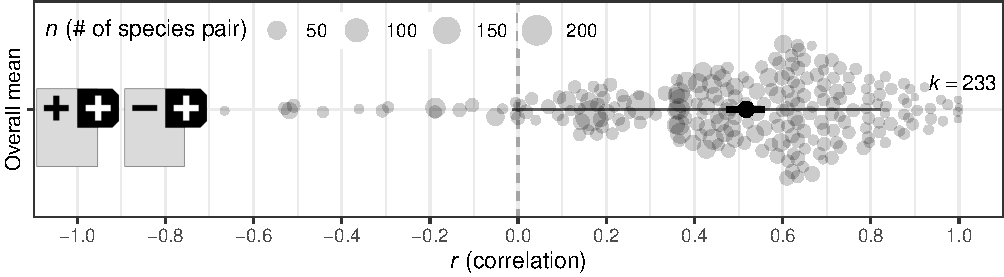
\includegraphics{Supporting_Information_files/figure-latex/unnamed-chunk-12-1.pdf}

\begin{Shaded}
\begin{Highlighting}[]
\CommentTok{# for Fig 3}

\NormalTok{a <-}\StringTok{ }\KeywordTok{ggplot}\NormalTok{(}\DataTypeTok{data =}\NormalTok{ effect_ma, }\KeywordTok{aes}\NormalTok{(}\DataTypeTok{x =} \KeywordTok{tanh}\NormalTok{(estimate), }\DataTypeTok{y =} \StringTok{"Overall mean"}\NormalTok{)) }\OperatorTok{+}\StringTok{ }\KeywordTok{scale_x_continuous}\NormalTok{(}\DataTypeTok{limits =} \KeywordTok{c}\NormalTok{(}\OperatorTok{-}\DecValTok{1}\NormalTok{, }
    \DecValTok{1}\NormalTok{), }\DataTypeTok{breaks =} \KeywordTok{seq}\NormalTok{(}\OperatorTok{-}\DecValTok{1}\NormalTok{, }\DecValTok{1}\NormalTok{, }\DataTypeTok{by =} \FloatTok{0.2}\NormalTok{)) }\OperatorTok{+}\StringTok{ }\KeywordTok{geom_quasirandom}\NormalTok{(}\DataTypeTok{data =}\NormalTok{ dat, }\KeywordTok{aes}\NormalTok{(}\DataTypeTok{x =} \KeywordTok{tanh}\NormalTok{(Zr), }
    \DataTypeTok{y =} \StringTok{"Overall mean"}\NormalTok{, }\DataTypeTok{size =}\NormalTok{ (}\DecValTok{1}\OperatorTok{/}\NormalTok{VZr) }\OperatorTok{+}\StringTok{ }\DecValTok{3}\NormalTok{), }\DataTypeTok{groupOnX =} \OtherTok{FALSE}\NormalTok{, }\DataTypeTok{alpha =} \FloatTok{0.2}\NormalTok{) }\OperatorTok{+}\StringTok{ }\CommentTok{# precition interval (PI)}
\KeywordTok{geom_errorbarh}\NormalTok{(}\KeywordTok{aes}\NormalTok{(}\DataTypeTok{xmin =} \KeywordTok{tanh}\NormalTok{(lowerPR), }\DataTypeTok{xmax =} \KeywordTok{tanh}\NormalTok{(upperPR)), }\DataTypeTok{height =} \DecValTok{0}\NormalTok{, }\DataTypeTok{show.legend =}\NormalTok{ F, }
    \DataTypeTok{size =} \FloatTok{0.5}\NormalTok{, }\DataTypeTok{alpha =} \FloatTok{0.6}\NormalTok{) }\OperatorTok{+}\StringTok{ }\CommentTok{# CI}
\KeywordTok{geom_errorbarh}\NormalTok{(}\KeywordTok{aes}\NormalTok{(}\DataTypeTok{xmin =} \KeywordTok{tanh}\NormalTok{(lowerCL), }\DataTypeTok{xmax =} \KeywordTok{tanh}\NormalTok{(upperCL)), }\DataTypeTok{height =} \DecValTok{0}\NormalTok{, }\DataTypeTok{show.legend =}\NormalTok{ F, }
    \DataTypeTok{size =} \FloatTok{1.2}\NormalTok{) }\OperatorTok{+}\StringTok{ }
\KeywordTok{geom_vline}\NormalTok{(}\DataTypeTok{xintercept =} \DecValTok{0}\NormalTok{, }\DataTypeTok{linetype =} \DecValTok{2}\NormalTok{, }\DataTypeTok{colour =} \StringTok{"black"}\NormalTok{, }\DataTypeTok{alpha =} \FloatTok{0.3}\NormalTok{) }\OperatorTok{+}\StringTok{ }\CommentTok{# creating dots and different size (bee-swarm and bubbles)}
\KeywordTok{geom_point}\NormalTok{(}\DataTypeTok{size =} \DecValTok{3}\NormalTok{, }\DataTypeTok{shape =} \DecValTok{21}\NormalTok{, }\DataTypeTok{fill =} \StringTok{"black"}\NormalTok{) }\OperatorTok{+}\StringTok{ }\KeywordTok{annotate}\NormalTok{(}\StringTok{"text"}\NormalTok{, }\DataTypeTok{x =} \FloatTok{0.93}\NormalTok{, }\DataTypeTok{y =} \FloatTok{1.15}\NormalTok{, }
    \DataTypeTok{label =} \KeywordTok{paste}\NormalTok{(}\StringTok{"italic(k)=="}\NormalTok{, }\KeywordTok{length}\NormalTok{(dat}\OperatorTok{$}\NormalTok{Zr)), }\DataTypeTok{parse =} \OtherTok{TRUE}\NormalTok{, }\DataTypeTok{hjust =} \StringTok{"left"}\NormalTok{, }\DataTypeTok{size =} \FloatTok{3.5}\NormalTok{) }\OperatorTok{+}\StringTok{ }
\StringTok{    }\KeywordTok{labs}\NormalTok{(}\DataTypeTok{x =} \StringTok{""}\NormalTok{, }\DataTypeTok{y =} \StringTok{""}\NormalTok{, }\DataTypeTok{size =} \KeywordTok{expression}\NormalTok{(}\KeywordTok{paste}\NormalTok{(}\KeywordTok{italic}\NormalTok{(n), }\StringTok{" (# of species pairs)"}\NormalTok{)), }
        \DataTypeTok{tag =} \StringTok{"a"}\NormalTok{) }\OperatorTok{+}\StringTok{ }\KeywordTok{theme_bw}\NormalTok{() }\OperatorTok{+}\StringTok{ }\KeywordTok{theme}\NormalTok{(}\DataTypeTok{legend.position =} \KeywordTok{c}\NormalTok{(}\DecValTok{0}\NormalTok{, }\DecValTok{1}\NormalTok{), }\DataTypeTok{legend.justification =} \KeywordTok{c}\NormalTok{(}\DecValTok{0}\NormalTok{, }
    \DecValTok{1}\NormalTok{)) }\OperatorTok{+}\StringTok{ }\KeywordTok{theme}\NormalTok{(}\DataTypeTok{legend.direction =} \StringTok{"horizontal"}\NormalTok{) }\OperatorTok{+}\StringTok{ }\CommentTok{# theme(legend.background = element_rect(fill = 'white', colour = 'black')) +}
\KeywordTok{theme}\NormalTok{(}\DataTypeTok{legend.background =} \KeywordTok{element_blank}\NormalTok{()) }\OperatorTok{+}\StringTok{ }\KeywordTok{theme}\NormalTok{(}\DataTypeTok{axis.text.y =} \KeywordTok{element_text}\NormalTok{(}\DataTypeTok{size =} \DecValTok{10}\NormalTok{, }
    \DataTypeTok{colour =} \StringTok{"black"}\NormalTok{, }\DataTypeTok{hjust =} \FloatTok{0.5}\NormalTok{, }\DataTypeTok{angle =} \DecValTok{90}\NormalTok{)) }\OperatorTok{+}\StringTok{ }\KeywordTok{annotation_custom}\NormalTok{(}\KeywordTok{rasterGrob}\NormalTok{(image_mutualism), }
    \DataTypeTok{xmin =} \FloatTok{-1.1}\NormalTok{, }\DataTypeTok{xmax =} \FloatTok{-0.9}\NormalTok{, }\DataTypeTok{ymin =} \FloatTok{0.6}\NormalTok{, }\DataTypeTok{ymax =} \FloatTok{1.2}\NormalTok{) }\OperatorTok{+}\StringTok{ }\KeywordTok{annotation_custom}\NormalTok{(}\KeywordTok{rasterGrob}\NormalTok{(image_parasitism), }
    \DataTypeTok{xmin =} \FloatTok{-0.9}\NormalTok{, }\DataTypeTok{xmax =} \FloatTok{-0.7}\NormalTok{, }\DataTypeTok{ymin =} \FloatTok{0.6}\NormalTok{, }\DataTypeTok{ymax =} \FloatTok{1.2}\NormalTok{)}
\end{Highlighting}
\end{Shaded}

\textbf{Figure 3a:} A forest plot showing the meta-analytic mean (mean
effect size) with its 95\% confidence interval (thick line) and 95\%
prediction interval (thin line), with observed effect sizes based on
various sample sizes.

\hypertarget{meta-regression}{%
\subsection{Meta-regression}\label{meta-regression}}

We ran a univariate meta-regression model for each of the following
moderators: 1) \texttt{symbiosis}, 2) \texttt{host\_tax\_broad}, 3)
\texttt{symbiont\_tax\_broad}, 4) \texttt{host\_range\_link\_ratio}, 5)
\texttt{host\_range\_taxonomic\_breadth}, 6)
\texttt{mode\_of\_transmission\_broad}, and 7) \texttt{endo\_or\_ecto}.
The results from these models are presented in the main text.

In addition to these, we ran three more univariate models: 1)
\texttt{host\_tax\_symbiosis} (equivalent to the interaction term
between \texttt{symbiosis} and \texttt{host\_tax\_symbiosis};
\texttt{symbiosis*host\_tax\_symbiosis}), 2)
\texttt{symbiont\_tax\_symbiosis}
(\texttt{symbiosis*symbiont\_tax\_broad}), 3)
\texttt{host\_symbiont\_tax}
(\texttt{host\_tax\_symbiosis*symbiont\_tax\_broad}) and 4)
\texttt{symbiosis\_transmission}
(\texttt{symbiosis*mode\_of\_transmission\_broad}). These moderators are
created below:

\begin{Shaded}
\begin{Highlighting}[]
\NormalTok{dat }\OperatorTok\StringTok{ }
\StringTok{    }\CommentTok{# host_tax_broad*symbiosis (host_tax_symbiosis) }
\StringTok{  }\KeywordTok{mutate}\NormalTok{(}\DataTypeTok{host_tax_symbiosis =} \KeywordTok{str_c}\NormalTok{(host_tax_broad, symbiosis), }
         \DataTypeTok{host_tax_symbiosis =} \KeywordTok{ifelse}\NormalTok{(host_tax_symbiosis }\OperatorTok{==}\StringTok{ "InvertNA"}\NormalTok{, }\OtherTok{NA}\NormalTok{, host_tax_symbiosis),}
         \DataTypeTok{host_tax_symbiosis =} \KeywordTok{factor}\NormalTok{(host_tax_symbiosis),}
         \CommentTok{# symbiont_tax_broad*symbiosis (symbiont_tax_symbiosis)     }
         \DataTypeTok{symbiont_tax_symbiosis =} \KeywordTok{factor}\NormalTok{(}\KeywordTok{str_c}\NormalTok{(symbiont_tax_broad, symbiosis)),}
         \CommentTok{# host_tax_broad*symbiont_tax_broad (host_symbiont_tax)     }
         \DataTypeTok{host_symbiont_tax  =} \KeywordTok{factor}\NormalTok{(}\KeywordTok{str_c}\NormalTok{(host_tax_broad, symbiont_tax_broad)),}
         \CommentTok{# symbiosis*mode_of_transmission_broad (symbiosis_transmission)}
         \DataTypeTok{symbiosis_transmission  =} \KeywordTok{factor}\NormalTok{(}\KeywordTok{str_c}\NormalTok{(symbiosis, mode_of_transmission_broad)),}
         \CommentTok{# whether p values were the smallest value given the number of randamization - limit_researched (Yes = 1, No = 0)}
         \DataTypeTok{limit_reached =} \KeywordTok{if_else}\NormalTok{(}\KeywordTok{abs}\NormalTok{((}\DecValTok{1}\OperatorTok{/}\NormalTok{p_value) }\OperatorTok{-}\StringTok{ }\NormalTok{no_randomizations) }\OperatorTok{<=}\StringTok{ }\DecValTok{1}\NormalTok{, }\DecValTok{1}\NormalTok{, }\DecValTok{0}\NormalTok{))}
\end{Highlighting}
\end{Shaded}

\hypertarget{univariate-uni-predictor-analyses}{%
\subsubsection{Univariate (uni-predictor)
analyses}\label{univariate-uni-predictor-analyses}}

We first conducted a series of meta-regression models with one
predictor.

\hypertarget{the-type-of-symbiosis-parasitism-vs.-mutualism}{%
\paragraph{The type of symbiosis: parasitism
vs.~mutualism}\label{the-type-of-symbiosis-parasitism-vs.-mutualism}}

\begin{Shaded}
\begin{Highlighting}[]
\CommentTok{# meta-regression: mutiple intercepts}
\NormalTok{mr_symbiosis1 <-}\StringTok{ }\KeywordTok{rma.mv}\NormalTok{(}\DataTypeTok{yi =}\NormalTok{ Zr, }\DataTypeTok{V =}\NormalTok{ VZr, }\DataTypeTok{mods =} \OperatorTok{~}\NormalTok{symbiosis }\OperatorTok{-}\StringTok{ }\DecValTok{1}\NormalTok{, }\DataTypeTok{test =} \StringTok{"t"}\NormalTok{, }\DataTypeTok{random =} \OperatorTok{~}\DecValTok{1} \OperatorTok{|}\StringTok{ }
\StringTok{    }\NormalTok{authors, }\DataTypeTok{data =}\NormalTok{ dat)}
\CommentTok{# meta-regression: contrast}
\NormalTok{mr_symbiosis2 <-}\StringTok{ }\KeywordTok{rma.mv}\NormalTok{(}\DataTypeTok{yi =}\NormalTok{ Zr, }\DataTypeTok{V =}\NormalTok{ VZr, }\DataTypeTok{mods =} \OperatorTok{~}\NormalTok{symbiosis, }\DataTypeTok{test =} \StringTok{"t"}\NormalTok{, }\DataTypeTok{random =} \OperatorTok{~}\DecValTok{1} \OperatorTok{|}\StringTok{ }
\StringTok{    }\NormalTok{authors, }\DataTypeTok{data =}\NormalTok{ dat)}
\end{Highlighting}
\end{Shaded}

\textbf{Supplementary Table 2:} Regression coefficients (Estimate), 95\%
confidence intervals (CIs), variance components (V) and variance
explained, \emph{R}\textsuperscript{2}\textsubscript{{[}marginal{]}}
(Nakagawa \& Schielzeth
\protect\hyperlink{ref-nakagawa2013general}{2013}) (R2) from the
meta-regression with \texttt{symbiosis}.

\begin{Shaded}
\begin{Highlighting}[]
\CommentTok{# getting marginal R2}
\NormalTok{r2_symbiosis1 <-}\StringTok{ }\KeywordTok{R2}\NormalTok{(mr_symbiosis1)}

\CommentTok{# getting estimates}
\NormalTok{res_symbiosis1 <-}\StringTok{ }\KeywordTok{get_est}\NormalTok{(mr_symbiosis1, }\DataTypeTok{mod =} \StringTok{"symbiosis"}\NormalTok{)}
\NormalTok{res_symbiosis2 <-}\StringTok{ }\KeywordTok{get_est}\NormalTok{(mr_symbiosis2, }\DataTypeTok{mod =} \StringTok{"symbiosis"}\NormalTok{)}

\CommentTok{# creating a table}
\KeywordTok{tibble}\NormalTok{(}\StringTok{`}\DataTypeTok{Fixed effect}\StringTok{`}\NormalTok{ =}\StringTok{ }\KeywordTok{c}\NormalTok{(}\KeywordTok{as.character}\NormalTok{(res_symbiosis1}\OperatorTok{$}\NormalTok{name), }\KeywordTok{cont_gen}\NormalTok{(res_symbiosis1}\OperatorTok{$}\NormalTok{name)), }
    \DataTypeTok{Estimate =} \KeywordTok{c}\NormalTok{(res_symbiosis1}\OperatorTok{$}\NormalTok{estimate, res_symbiosis2}\OperatorTok{$}\NormalTok{estimate[}\DecValTok{2}\NormalTok{]), }\StringTok{`}\DataTypeTok{Lower CI [0.025]}\StringTok{`}\NormalTok{ =}\StringTok{ }\KeywordTok{c}\NormalTok{(res_symbiosis1}\OperatorTok{$}\NormalTok{lowerCL, }
\NormalTok{        res_symbiosis2}\OperatorTok{$}\NormalTok{lowerCL[}\DecValTok{2}\NormalTok{]), }\StringTok{`}\DataTypeTok{Upper CI  [0.975]}\StringTok{`}\NormalTok{ =}\StringTok{ }\KeywordTok{c}\NormalTok{(res_symbiosis1}\OperatorTok{$}\NormalTok{upperCL, }
\NormalTok{        res_symbiosis2}\OperatorTok{$}\NormalTok{upperCL[}\DecValTok{2}\NormalTok{]), }\StringTok{`}\DataTypeTok{V[authors]}\StringTok{`}\NormalTok{ =}\StringTok{ }\KeywordTok{c}\NormalTok{(mr_symbiosis1}\OperatorTok{$}\NormalTok{sigma2, }\KeywordTok{rep}\NormalTok{(}\OtherTok{NA}\NormalTok{, }
        \DecValTok{2}\NormalTok{)), }\DataTypeTok{R2 =} \KeywordTok{c}\NormalTok{(r2_symbiosis1[}\DecValTok{1}\NormalTok{], }\KeywordTok{rep}\NormalTok{(}\OtherTok{NA}\NormalTok{, }\DecValTok{2}\NormalTok{))) }\OperatorTok\StringTok{ }\KeywordTok{kable}\NormalTok{(}\StringTok{"html"}\NormalTok{, }\DataTypeTok{digits =} \DecValTok{3}\NormalTok{) }\OperatorTok\StringTok{ }
\StringTok{    }\KeywordTok{kable_styling}\NormalTok{(}\StringTok{"striped"}\NormalTok{, }\DataTypeTok{position =} \StringTok{"left"}\NormalTok{)}
\end{Highlighting}
\end{Shaded}

Fixed effect

Estimate

Lower CI {[}0.025{]}

Upper CI {[}0.975{]}

V{[}authors{]}

R2

Mutualist

0.652

0.551

0.752

0.085

0.037

Parasite

0.529

0.457

0.601

NA

NA

Mutualist-Parasite

-0.123

-0.244

-0.002

NA

NA

\begin{Shaded}
\begin{Highlighting}[]
\CommentTok{# adding sample size (k) for each category}
\NormalTok{k_symbiosis <-}\StringTok{ }\NormalTok{dat }\OperatorTok\StringTok{ }\KeywordTok{group_by}\NormalTok{(symbiosis) }\OperatorTok\StringTok{ }\KeywordTok{count}\NormalTok{()}
\CommentTok{# getting estimates and predicitons}
\NormalTok{pred_symbiosis <-}\StringTok{ }\KeywordTok{get_pred}\NormalTok{(mr_symbiosis1, }\DataTypeTok{mod =} \StringTok{"symbiosis"}\NormalTok{) }
\NormalTok{res_symbiosis1 <-}\StringTok{ }\KeywordTok{left_join}\NormalTok{(res_symbiosis1, k_symbiosis, }\DataTypeTok{by =}  \KeywordTok{c}\NormalTok{(}\StringTok{"name"}\NormalTok{ =}\StringTok{ "symbiosis"}\NormalTok{))  }\OperatorTok\StringTok{ }\KeywordTok{left_join}\NormalTok{(pred_symbiosis)}
\CommentTok{#res_symbiosis1 }
\CommentTok{# drawing a funnel plot - fig 2b}
\NormalTok{fig_symbiosis <-}\StringTok{ }\KeywordTok{ggplot}\NormalTok{(}\DataTypeTok{data =}\NormalTok{ res_symbiosis1, }\KeywordTok{aes}\NormalTok{(}\DataTypeTok{x =} \KeywordTok{tanh}\NormalTok{(estimate), }\DataTypeTok{y =}\NormalTok{ name)) }\OperatorTok{+}
\StringTok{  }\KeywordTok{scale_x_continuous}\NormalTok{(}\DataTypeTok{limits=}\KeywordTok{c}\NormalTok{(}\OperatorTok{-}\DecValTok{1}\NormalTok{, }\DecValTok{1}\NormalTok{), }\DataTypeTok{breaks =} \KeywordTok{seq}\NormalTok{(}\OperatorTok{-}\DecValTok{1}\NormalTok{, }\DecValTok{1}\NormalTok{, }\DataTypeTok{by =} \FloatTok{0.2}\NormalTok{) ) }\OperatorTok{+}
\StringTok{  }\KeywordTok{geom_quasirandom}\NormalTok{(}\DataTypeTok{data =}\NormalTok{ dat }\OperatorTok\StringTok{ }\KeywordTok{filter}\NormalTok{(}\OperatorTok{!}\KeywordTok{is.na}\NormalTok{(symbiosis)), }
                   \KeywordTok{aes}\NormalTok{(}\DataTypeTok{x=} \KeywordTok{tanh}\NormalTok{(Zr), }\DataTypeTok{y =}\NormalTok{ symbiosis, }\DataTypeTok{size =}\NormalTok{ ((}\DecValTok{1}\OperatorTok{/}\NormalTok{VZr) }\OperatorTok{+}\StringTok{ }\DecValTok{3}\NormalTok{), }\DataTypeTok{colour =}\NormalTok{ symbiosis), }\DataTypeTok{groupOnX =} \OtherTok{FALSE}\NormalTok{, }\DataTypeTok{alpha=}\FloatTok{0.2}\NormalTok{) }\OperatorTok{+}\StringTok{ }
\StringTok{  }\CommentTok{# 95 %precition interval (PI)}
\StringTok{  }\KeywordTok{geom_errorbarh}\NormalTok{(}\KeywordTok{aes}\NormalTok{(}\DataTypeTok{xmin =} \KeywordTok{tanh}\NormalTok{(lowerPR), }\DataTypeTok{xmax =} \KeywordTok{tanh}\NormalTok{(upperPR)),  }\DataTypeTok{height =} \DecValTok{0}\NormalTok{, }\DataTypeTok{show.legend =}\NormalTok{ F, }\DataTypeTok{size =} \FloatTok{0.5}\NormalTok{, }\DataTypeTok{alpha =} \FloatTok{0.6}\NormalTok{) }\OperatorTok{+}
\StringTok{  }\CommentTok{# 95 %CI}
\StringTok{  }\KeywordTok{geom_errorbarh}\NormalTok{(}\KeywordTok{aes}\NormalTok{(}\DataTypeTok{xmin =} \KeywordTok{tanh}\NormalTok{(lowerCL), }\DataTypeTok{xmax =} \KeywordTok{tanh}\NormalTok{(upperCL)),  }\DataTypeTok{height =} \DecValTok{0}\NormalTok{, }\DataTypeTok{show.legend =}\NormalTok{ F, }\DataTypeTok{size =} \FloatTok{1.2}\NormalTok{) }\OperatorTok{+}
\StringTok{  }\KeywordTok{geom_vline}\NormalTok{(}\DataTypeTok{xintercept =} \DecValTok{0}\NormalTok{, }\DataTypeTok{linetype =} \DecValTok{2}\NormalTok{, }\DataTypeTok{colour =} \StringTok{"black"}\NormalTok{, }\DataTypeTok{alpha =} \FloatTok{0.3}\NormalTok{) }\OperatorTok{+}
\StringTok{  }\CommentTok{# creating dots and different size (bee-swarm and bubbles)}
\StringTok{  }\KeywordTok{geom_point}\NormalTok{(}\KeywordTok{aes}\NormalTok{(}\DataTypeTok{fill =}\NormalTok{ name), }\DataTypeTok{size =} \DecValTok{3}\NormalTok{, }\DataTypeTok{shape =} \DecValTok{21}\NormalTok{) }\OperatorTok{+}\StringTok{ }\CommentTok{#}
\StringTok{  }\CommentTok{# setting colours}
\StringTok{  }\KeywordTok{scale_color_manual}\NormalTok{(}\DataTypeTok{values =} \KeywordTok{c}\NormalTok{(}\StringTok{"Mutualist"}\NormalTok{ =}\StringTok{ "#E69F00"}\NormalTok{, }\StringTok{"Parasite"}\NormalTok{ =}\StringTok{ "#56B4E9"}\NormalTok{)) }\OperatorTok{+}
\StringTok{  }\KeywordTok{scale_fill_manual}\NormalTok{(}\DataTypeTok{values =} \KeywordTok{c}\NormalTok{(}\StringTok{"Mutualist"}\NormalTok{ =}\StringTok{ "#E69F00"}\NormalTok{, }\StringTok{"Parasite"}\NormalTok{ =}\StringTok{ "#56B4E9"}\NormalTok{)) }\OperatorTok{+}
\StringTok{  }\KeywordTok{annotate}\NormalTok{(}\StringTok{'text'}\NormalTok{, }\DataTypeTok{x =} \FloatTok{0.93}\NormalTok{, }\DataTypeTok{y =} \KeywordTok{c}\NormalTok{(}\FloatTok{1.15}\NormalTok{, }\FloatTok{2.15}\NormalTok{), }\DataTypeTok{label=} \KeywordTok{paste}\NormalTok{(}\StringTok{"italic(k)=="}\NormalTok{, res_symbiosis1}\OperatorTok{$}\NormalTok{n), }\DataTypeTok{parse =} \OtherTok{TRUE}\NormalTok{, }\DataTypeTok{hjust =} \StringTok{"left"}\NormalTok{, }\DataTypeTok{size =} \FloatTok{3.5}\NormalTok{) }\OperatorTok{+}
\StringTok{  }\KeywordTok{labs}\NormalTok{(}\DataTypeTok{x =} \KeywordTok{expression}\NormalTok{(}\KeywordTok{paste}\NormalTok{(}\KeywordTok{italic}\NormalTok{(r), }\StringTok{" (correlation)"}\NormalTok{)), }\DataTypeTok{y =} \StringTok{""}\NormalTok{, }\DataTypeTok{size =} \KeywordTok{expression}\NormalTok{(}\KeywordTok{paste}\NormalTok{(}\KeywordTok{italic}\NormalTok{(n), }\StringTok{" (# of species pairs)"}\NormalTok{)) ) }\OperatorTok{+}
\StringTok{  }\KeywordTok{guides}\NormalTok{(}\DataTypeTok{fill =} \StringTok{"none"}\NormalTok{, }\DataTypeTok{colour =} \StringTok{"none"}\NormalTok{) }\OperatorTok{+}
\StringTok{  }\KeywordTok{theme_bw}\NormalTok{() }\OperatorTok{+}
\StringTok{  }\KeywordTok{theme}\NormalTok{(}\DataTypeTok{legend.position=} \KeywordTok{c}\NormalTok{(}\DecValTok{0}\NormalTok{, }\DecValTok{1}\NormalTok{), }\DataTypeTok{legend.justification =} \KeywordTok{c}\NormalTok{(}\DecValTok{0}\NormalTok{,}\DecValTok{1}\NormalTok{)) }\OperatorTok{+}
\StringTok{  }\KeywordTok{theme}\NormalTok{(}\DataTypeTok{legend.direction=}\StringTok{"horizontal"}\NormalTok{) }\OperatorTok{+}
\StringTok{  }\CommentTok{#theme(legend.background = element_rect(fill = "white", colour = "black")) +}
\StringTok{  }\KeywordTok{theme}\NormalTok{(}\DataTypeTok{legend.background =} \KeywordTok{element_blank}\NormalTok{()) }\OperatorTok{+}
\StringTok{  }\KeywordTok{theme}\NormalTok{(}\DataTypeTok{axis.text.y =} \KeywordTok{element_text}\NormalTok{(}\DataTypeTok{size =} \DecValTok{10}\NormalTok{, }\DataTypeTok{colour =}\StringTok{"black"}\NormalTok{, }\DataTypeTok{hjust =} \FloatTok{0.5}\NormalTok{, }\DataTypeTok{angle =} \DecValTok{90}\NormalTok{)) }\OperatorTok{+}
\StringTok{  }\CommentTok{# putting pictures in}
\StringTok{  }\KeywordTok{annotation_custom}\NormalTok{(}\KeywordTok{rasterGrob}\NormalTok{(image_mutualism), }\DataTypeTok{xmin =} \DecValTok{-1}\NormalTok{, }\DataTypeTok{xmax =} \FloatTok{-0.8}\NormalTok{, }\DataTypeTok{ymin =} \FloatTok{0.6}\NormalTok{, }\DataTypeTok{ymax =} \FloatTok{1.2}\NormalTok{) }\OperatorTok{+}\StringTok{ }
\StringTok{  }\KeywordTok{annotation_custom}\NormalTok{(}\KeywordTok{rasterGrob}\NormalTok{(image_parasitism), }\DataTypeTok{xmin =} \DecValTok{-1}\NormalTok{, }\DataTypeTok{xmax =} \FloatTok{-0.8}\NormalTok{, }\DataTypeTok{ymin =} \FloatTok{1.6}\NormalTok{, }\DataTypeTok{ymax =} \FloatTok{2.2}\NormalTok{)}

\NormalTok{fig_symbiosis}
\end{Highlighting}
\end{Shaded}

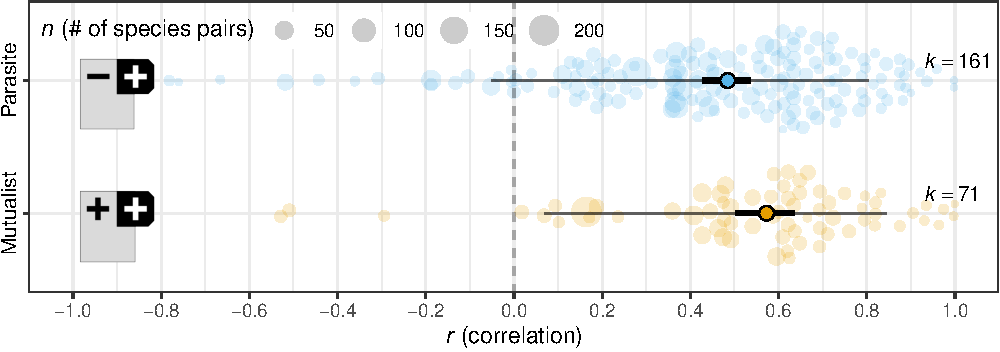
\includegraphics{Supporting_Information_files/figure-latex/unnamed-chunk-16-1.pdf}

\begin{Shaded}
\begin{Highlighting}[]
\CommentTok{# fig 3}

\NormalTok{b <-}\StringTok{ }\KeywordTok{ggplot}\NormalTok{(}\DataTypeTok{data =}\NormalTok{ res_symbiosis1, }\KeywordTok{aes}\NormalTok{(}\DataTypeTok{x =} \KeywordTok{tanh}\NormalTok{(estimate), }\DataTypeTok{y =}\NormalTok{ name)) }\OperatorTok{+}
\StringTok{  }\KeywordTok{scale_x_continuous}\NormalTok{(}\DataTypeTok{limits=}\KeywordTok{c}\NormalTok{(}\OperatorTok{-}\DecValTok{1}\NormalTok{, }\DecValTok{1}\NormalTok{), }\DataTypeTok{breaks =} \KeywordTok{seq}\NormalTok{(}\OperatorTok{-}\DecValTok{1}\NormalTok{, }\DecValTok{1}\NormalTok{, }\DataTypeTok{by =} \FloatTok{0.2}\NormalTok{) ) }\OperatorTok{+}
\StringTok{  }\KeywordTok{geom_quasirandom}\NormalTok{(}\DataTypeTok{data =}\NormalTok{ dat }\OperatorTok\StringTok{ }\KeywordTok{filter}\NormalTok{(}\OperatorTok{!}\KeywordTok{is.na}\NormalTok{(symbiosis)), }
                   \KeywordTok{aes}\NormalTok{(}\DataTypeTok{x=} \KeywordTok{tanh}\NormalTok{(Zr), }\DataTypeTok{y =}\NormalTok{ symbiosis, }\DataTypeTok{size =}\NormalTok{ ((}\DecValTok{1}\OperatorTok{/}\NormalTok{VZr) }\OperatorTok{+}\StringTok{ }\DecValTok{3}\NormalTok{), }\DataTypeTok{colour =}\NormalTok{ symbiosis), }\DataTypeTok{groupOnX =} \OtherTok{FALSE}\NormalTok{, }\DataTypeTok{alpha=}\FloatTok{0.2}\NormalTok{) }\OperatorTok{+}\StringTok{ }
\StringTok{  }\CommentTok{# 95 %precition interval (PI)}
\StringTok{  }\KeywordTok{geom_errorbarh}\NormalTok{(}\KeywordTok{aes}\NormalTok{(}\DataTypeTok{xmin =} \KeywordTok{tanh}\NormalTok{(lowerPR), }\DataTypeTok{xmax =} \KeywordTok{tanh}\NormalTok{(upperPR)),  }\DataTypeTok{height =} \DecValTok{0}\NormalTok{, }\DataTypeTok{show.legend =}\NormalTok{ F, }\DataTypeTok{size =} \FloatTok{0.5}\NormalTok{, }\DataTypeTok{alpha =} \FloatTok{0.6}\NormalTok{) }\OperatorTok{+}
\StringTok{  }\CommentTok{# 95 %CI}
\StringTok{  }\KeywordTok{geom_errorbarh}\NormalTok{(}\KeywordTok{aes}\NormalTok{(}\DataTypeTok{xmin =} \KeywordTok{tanh}\NormalTok{(lowerCL), }\DataTypeTok{xmax =} \KeywordTok{tanh}\NormalTok{(upperCL)),  }\DataTypeTok{height =} \DecValTok{0}\NormalTok{, }\DataTypeTok{show.legend =}\NormalTok{ F, }\DataTypeTok{size =} \FloatTok{1.2}\NormalTok{) }\OperatorTok{+}
\StringTok{  }\KeywordTok{geom_vline}\NormalTok{(}\DataTypeTok{xintercept =} \DecValTok{0}\NormalTok{, }\DataTypeTok{linetype =} \DecValTok{2}\NormalTok{, }\DataTypeTok{colour =} \StringTok{"black"}\NormalTok{, }\DataTypeTok{alpha =} \FloatTok{0.3}\NormalTok{) }\OperatorTok{+}
\StringTok{  }\CommentTok{# creating dots and different size (bee-swarm and bubbles)}
\StringTok{  }\KeywordTok{geom_point}\NormalTok{(}\KeywordTok{aes}\NormalTok{(}\DataTypeTok{fill =}\NormalTok{ name), }\DataTypeTok{size =} \DecValTok{3}\NormalTok{, }\DataTypeTok{shape =} \DecValTok{21}\NormalTok{) }\OperatorTok{+}\StringTok{ }\CommentTok{#}
\StringTok{  }\CommentTok{# setting colours}
\StringTok{  }\KeywordTok{scale_color_manual}\NormalTok{(}\DataTypeTok{values =} \KeywordTok{c}\NormalTok{(}\StringTok{"Mutualist"}\NormalTok{ =}\StringTok{ "#E69F00"}\NormalTok{, }\StringTok{"Parasite"}\NormalTok{ =}\StringTok{ "#56B4E9"}\NormalTok{)) }\OperatorTok{+}
\StringTok{  }\KeywordTok{scale_fill_manual}\NormalTok{(}\DataTypeTok{values =} \KeywordTok{c}\NormalTok{(}\StringTok{"Mutualist"}\NormalTok{ =}\StringTok{ "#E69F00"}\NormalTok{, }\StringTok{"Parasite"}\NormalTok{ =}\StringTok{ "#56B4E9"}\NormalTok{)) }\OperatorTok{+}
\StringTok{  }\KeywordTok{annotate}\NormalTok{(}\StringTok{'text'}\NormalTok{, }\DataTypeTok{x =} \FloatTok{0.93}\NormalTok{, }\DataTypeTok{y =} \KeywordTok{c}\NormalTok{(}\FloatTok{1.15}\NormalTok{, }\FloatTok{2.15}\NormalTok{), }\DataTypeTok{label=} \KeywordTok{paste}\NormalTok{(}\StringTok{"italic(k)=="}\NormalTok{, res_symbiosis1}\OperatorTok{$}\NormalTok{n), }\DataTypeTok{parse =} \OtherTok{TRUE}\NormalTok{, }\DataTypeTok{hjust =} \StringTok{"left"}\NormalTok{, }\DataTypeTok{size =} \FloatTok{3.5}\NormalTok{) }\OperatorTok{+}
\StringTok{  }\KeywordTok{labs}\NormalTok{(}\DataTypeTok{x =} \StringTok{""}\NormalTok{, }\DataTypeTok{y =} \StringTok{""}\NormalTok{, }\DataTypeTok{tag =} \StringTok{"b"}\NormalTok{) }\OperatorTok{+}
\StringTok{  }\KeywordTok{guides}\NormalTok{(}\DataTypeTok{fill =} \StringTok{"none"}\NormalTok{, }\DataTypeTok{colour =} \StringTok{"none"}\NormalTok{) }\OperatorTok{+}
\StringTok{  }\KeywordTok{theme_bw}\NormalTok{() }\OperatorTok{+}
\StringTok{  }\KeywordTok{theme}\NormalTok{(}\DataTypeTok{legend.position=}\StringTok{"none"}\NormalTok{) }\OperatorTok{+}
\StringTok{  }\KeywordTok{theme}\NormalTok{(}\DataTypeTok{axis.text.y =} \KeywordTok{element_text}\NormalTok{(}\DataTypeTok{size =} \DecValTok{10}\NormalTok{, }\DataTypeTok{colour =}\StringTok{"black"}\NormalTok{,}\DataTypeTok{hjust =} \FloatTok{0.5}\NormalTok{, }\DataTypeTok{angle =} \DecValTok{90}\NormalTok{)) }\OperatorTok{+}
\StringTok{  }\CommentTok{# putting pictures in}
\StringTok{  }\KeywordTok{annotation_custom}\NormalTok{(}\KeywordTok{rasterGrob}\NormalTok{(image_mutualism), }\DataTypeTok{xmin =} \DecValTok{-1}\NormalTok{, }\DataTypeTok{xmax =} \FloatTok{-0.8}\NormalTok{, }\DataTypeTok{ymin =} \FloatTok{0.6}\NormalTok{, }\DataTypeTok{ymax =} \FloatTok{1.2}\NormalTok{) }\OperatorTok{+}\StringTok{ }
\StringTok{  }\KeywordTok{annotation_custom}\NormalTok{(}\KeywordTok{rasterGrob}\NormalTok{(image_parasitism), }\DataTypeTok{xmin =} \DecValTok{-1}\NormalTok{, }\DataTypeTok{xmax =} \FloatTok{-0.8}\NormalTok{, }\DataTypeTok{ymin =} \FloatTok{1.6}\NormalTok{, }\DataTypeTok{ymax =} \FloatTok{2.2}\NormalTok{)}
\end{Highlighting}
\end{Shaded}

\textbf{Figure 3b:} A forest plot showing the group-wise means (the
categorical variable \texttt{symbiosis}) with their 95\% confidence
intervals (thick lines) and 95\% prediction intervals (thin lines), with
observed effect sizes based on various sample sizes.

\hypertarget{the-effect-of-host-taxa}{%
\paragraph{The effect of host taxa}\label{the-effect-of-host-taxa}}

\begin{Shaded}
\begin{Highlighting}[]
\CommentTok{# reordering}
\NormalTok{dat}\OperatorTok{$}\NormalTok{host_tax_broad <-}\StringTok{ }\KeywordTok{factor}\NormalTok{(dat}\OperatorTok{$}\NormalTok{host_tax_broad, }\DataTypeTok{levels =} \KeywordTok{c}\NormalTok{(}\StringTok{"Microbe"}\NormalTok{, }\StringTok{"Plant"}\NormalTok{, }\StringTok{"Invert"}\NormalTok{, }
    \StringTok{"Vert"}\NormalTok{))}

\CommentTok{# meta-regression: mutiple intercepts}
\NormalTok{mr_host_tax_broad1 <-}\StringTok{ }\KeywordTok{rma.mv}\NormalTok{(}\DataTypeTok{yi =}\NormalTok{ Zr, }\DataTypeTok{V =}\NormalTok{ VZr, }\DataTypeTok{mods =} \OperatorTok{~}\NormalTok{host_tax_broad }\OperatorTok{-}\StringTok{ }\DecValTok{1}\NormalTok{, }\DataTypeTok{test =} \StringTok{"t"}\NormalTok{, }
    \DataTypeTok{random =} \OperatorTok{~}\DecValTok{1} \OperatorTok{|}\StringTok{ }\NormalTok{authors, }\DataTypeTok{data =}\NormalTok{ dat)}

\CommentTok{# meta-regression: contrast 1}
\NormalTok{mr_host_tax_broad2 <-}\StringTok{ }\KeywordTok{rma.mv}\NormalTok{(}\DataTypeTok{yi =}\NormalTok{ Zr, }\DataTypeTok{V =}\NormalTok{ VZr, }\DataTypeTok{mods =} \OperatorTok{~}\NormalTok{host_tax_broad, }\DataTypeTok{test =} \StringTok{"t"}\NormalTok{, }
    \DataTypeTok{random =} \OperatorTok{~}\DecValTok{1} \OperatorTok{|}\StringTok{ }\NormalTok{authors, }\DataTypeTok{data =}\NormalTok{ dat)}

\CommentTok{# meta-regression: contrast 2}
\NormalTok{mr_host_tax_broad3 <-}\StringTok{ }\KeywordTok{rma.mv}\NormalTok{(}\DataTypeTok{yi =}\NormalTok{ Zr, }\DataTypeTok{V =}\NormalTok{ VZr, }\DataTypeTok{mods =} \OperatorTok{~}\KeywordTok{relevel}\NormalTok{(host_tax_broad, }\DataTypeTok{ref =} \StringTok{"Plant"}\NormalTok{), }
    \DataTypeTok{test =} \StringTok{"t"}\NormalTok{, }\DataTypeTok{random =} \OperatorTok{~}\DecValTok{1} \OperatorTok{|}\StringTok{ }\NormalTok{authors, }\DataTypeTok{data =}\NormalTok{ dat)}

\CommentTok{# meta-regression: contrast 3}
\NormalTok{mr_host_tax_broad4 <-}\StringTok{ }\KeywordTok{rma.mv}\NormalTok{(}\DataTypeTok{yi =}\NormalTok{ Zr, }\DataTypeTok{V =}\NormalTok{ VZr, }\DataTypeTok{mods =} \OperatorTok{~}\KeywordTok{relevel}\NormalTok{(host_tax_broad, }\DataTypeTok{ref =} \StringTok{"Invert"}\NormalTok{), }
    \DataTypeTok{test =} \StringTok{"t"}\NormalTok{, }\DataTypeTok{random =} \OperatorTok{~}\DecValTok{1} \OperatorTok{|}\StringTok{ }\NormalTok{authors, }\DataTypeTok{data =}\NormalTok{ dat)}
\end{Highlighting}
\end{Shaded}

\textbf{Supplementary Table 3:} Regression coefficients (estimate), 95\%
confidence intervals (CIs), variance components (V) and variance
explained, \emph{R}\textsuperscript{2}\textsubscript{{[}marginal{]}}
(R2) from the meta-regression with \texttt{host\_tax\_broad}.

\begin{Shaded}
\begin{Highlighting}[]
\CommentTok{# getting marginal R2}
\NormalTok{r2_host_tax_broad1 <-}\StringTok{ }\KeywordTok{R2}\NormalTok{(mr_host_tax_broad1)}

\CommentTok{# getting estimates}
\NormalTok{res_host_tax_broad1 <-}\StringTok{ }\KeywordTok{get_est}\NormalTok{(mr_host_tax_broad1, }\DataTypeTok{mod =} \StringTok{"host_tax_broad"}\NormalTok{)}
\NormalTok{res_host_tax_broad2 <-}\StringTok{ }\KeywordTok{get_est}\NormalTok{(mr_host_tax_broad2, }\DataTypeTok{mod =} \StringTok{"host_tax_broad"}\NormalTok{)}
\CommentTok{# the name bit does not work if relevel....}
\NormalTok{res_host_tax_broad3 <-}\StringTok{ }\KeywordTok{get_est}\NormalTok{(mr_host_tax_broad3, }\DataTypeTok{mod =} \StringTok{"host_tax_broad"}\NormalTok{)}
\NormalTok{res_host_tax_broad4 <-}\StringTok{ }\KeywordTok{get_est}\NormalTok{(mr_host_tax_broad4, }\DataTypeTok{mod =} \StringTok{"host_tax_broad"}\NormalTok{)}

\CommentTok{# creating a table}
\KeywordTok{tibble}\NormalTok{(}\StringTok{`}\DataTypeTok{Fixed effect}\StringTok{`}\NormalTok{ =}\StringTok{ }\KeywordTok{c}\NormalTok{(}\KeywordTok{as.character}\NormalTok{(res_host_tax_broad1}\OperatorTok{$}\NormalTok{name), }\KeywordTok{cont_gen}\NormalTok{(res_host_tax_broad1}\OperatorTok{$}\NormalTok{name)), }
    \DataTypeTok{Estimate =} \KeywordTok{c}\NormalTok{(res_host_tax_broad1}\OperatorTok{$}\NormalTok{estimate, res_host_tax_broad2}\OperatorTok{$}\NormalTok{estimate[}\OperatorTok{-}\DecValTok{1}\NormalTok{], }
\NormalTok{        res_host_tax_broad3}\OperatorTok{$}\NormalTok{estimate[}\OperatorTok{-}\NormalTok{(}\DecValTok{1}\OperatorTok{:}\DecValTok{2}\NormalTok{)], res_host_tax_broad4}\OperatorTok{$}\NormalTok{estimate[}\OperatorTok{-}\NormalTok{(}\DecValTok{1}\OperatorTok{:}\DecValTok{3}\NormalTok{)]), }
    \StringTok{`}\DataTypeTok{Lower CI [0.025]}\StringTok{`}\NormalTok{ =}\StringTok{ }\KeywordTok{c}\NormalTok{(res_host_tax_broad1}\OperatorTok{$}\NormalTok{lowerCL, res_host_tax_broad2}\OperatorTok{$}\NormalTok{lowerCL[}\OperatorTok{-}\DecValTok{1}\NormalTok{], }
\NormalTok{        res_host_tax_broad3}\OperatorTok{$}\NormalTok{lowerCL[}\OperatorTok{-}\NormalTok{(}\DecValTok{1}\OperatorTok{:}\DecValTok{2}\NormalTok{)], res_host_tax_broad4}\OperatorTok{$}\NormalTok{lowerCL[}\OperatorTok{-}\NormalTok{(}\DecValTok{1}\OperatorTok{:}\DecValTok{3}\NormalTok{)]), }
    \StringTok{`}\DataTypeTok{Upper CI  [0.975]}\StringTok{`}\NormalTok{ =}\StringTok{ }\KeywordTok{c}\NormalTok{(res_host_tax_broad1}\OperatorTok{$}\NormalTok{upperCL, res_host_tax_broad2}\OperatorTok{$}\NormalTok{upperCL[}\OperatorTok{-}\DecValTok{1}\NormalTok{], }
\NormalTok{        res_host_tax_broad3}\OperatorTok{$}\NormalTok{upperCL[}\OperatorTok{-}\NormalTok{(}\DecValTok{1}\OperatorTok{:}\DecValTok{2}\NormalTok{)], res_host_tax_broad4}\OperatorTok{$}\NormalTok{upperCL[}\OperatorTok{-}\NormalTok{(}\DecValTok{1}\OperatorTok{:}\DecValTok{3}\NormalTok{)]), }
    \StringTok{`}\DataTypeTok{V[authors]}\StringTok{`}\NormalTok{ =}\StringTok{ }\KeywordTok{c}\NormalTok{(mr_host_tax_broad1}\OperatorTok{$}\NormalTok{sigma2, }\KeywordTok{rep}\NormalTok{(}\OtherTok{NA}\NormalTok{, }\DecValTok{9}\NormalTok{)), }\DataTypeTok{R2 =} \KeywordTok{c}\NormalTok{(r2_host_tax_broad1[}\DecValTok{1}\NormalTok{], }
        \KeywordTok{rep}\NormalTok{(}\OtherTok{NA}\NormalTok{, }\DecValTok{9}\NormalTok{))) }\OperatorTok\StringTok{ }\KeywordTok{kable}\NormalTok{(}\StringTok{"html"}\NormalTok{, }\DataTypeTok{digits =} \DecValTok{3}\NormalTok{) }\OperatorTok\StringTok{ }\KeywordTok{kable_styling}\NormalTok{(}\StringTok{"striped"}\NormalTok{, }\DataTypeTok{position =} \StringTok{"left"}\NormalTok{) }\OperatorTok\StringTok{ }
\StringTok{    }\KeywordTok{scroll_box}\NormalTok{(}\DataTypeTok{width =} \StringTok{"100%"}\NormalTok{, }\DataTypeTok{height =} \StringTok{"300px"}\NormalTok{)}
\end{Highlighting}
\end{Shaded}

Fixed effect

Estimate

Lower CI {[}0.025{]}

Upper CI {[}0.975{]}

V{[}authors{]}

R2

Microbe

0.910

0.659

1.160

0.084

0.143

Plant

0.408

0.280

0.536

NA

NA

Invert

0.649

0.538

0.761

NA

NA

Vert

0.561

0.475

0.647

NA

NA

Microbe-Plant

-0.502

-0.783

-0.220

NA

NA

Microbe-Invert

-0.261

-0.535

0.014

NA

NA

Microbe-Vert

-0.349

-0.613

-0.084

NA

NA

Plant-Invert

0.241

0.071

0.411

NA

NA

Plant-Vert

0.153

-0.001

0.308

NA

NA

Invert-Vert

-0.088

-0.226

0.050

NA

NA

\begin{Shaded}
\begin{Highlighting}[]
\CommentTok{# getting images}
\NormalTok{image_invertebrate_host <-}\StringTok{ }\KeywordTok{readPNG}\NormalTok{(}\KeywordTok{here}\NormalTok{(}\StringTok{"images/invertebrate_host_transparentbg.png"}\NormalTok{))}
\NormalTok{image_microbe_host <-}\StringTok{ }\KeywordTok{readPNG}\NormalTok{(}\KeywordTok{here}\NormalTok{(}\StringTok{"images/microbe_host_transparentbg.png"}\NormalTok{))}
\NormalTok{image_vertebrate_host <-}\StringTok{ }\KeywordTok{readPNG}\NormalTok{(}\KeywordTok{here}\NormalTok{(}\StringTok{"images/vertebrate_host_transparentbg.png"}\NormalTok{))}
\NormalTok{image_plant_host <-}\StringTok{ }\KeywordTok{readPNG}\NormalTok{(}\KeywordTok{here}\NormalTok{(}\StringTok{"images/plant_host_transparentbg.png"}\NormalTok{))}

\CommentTok{# adding sample size (k) for each category}
\NormalTok{k_host_tax_broad <-}\StringTok{ }\NormalTok{dat }\OperatorTok\StringTok{ }\KeywordTok{group_by}\NormalTok{(host_tax_broad) }\OperatorTok\StringTok{ }\KeywordTok{count}\NormalTok{()}
\CommentTok{# getting estimates and predicitons}
\NormalTok{pred_host_tax_broad <-}\StringTok{ }\KeywordTok{get_pred}\NormalTok{(mr_host_tax_broad1, }\DataTypeTok{mod =} \StringTok{"host_tax_broad"}\NormalTok{) }
\NormalTok{res_host_tax_broad1 <-}\StringTok{ }\KeywordTok{left_join}\NormalTok{(res_host_tax_broad1, k_host_tax_broad, }\DataTypeTok{by =}  \KeywordTok{c}\NormalTok{(}\StringTok{"name"}\NormalTok{ =}\StringTok{ "host_tax_broad"}\NormalTok{))  }\OperatorTok\StringTok{ }\KeywordTok{left_join}\NormalTok{(pred_host_tax_broad)}
\CommentTok{#res_symbiosis1 }
\CommentTok{# drawing a funnel plot - fig 2b}
\NormalTok{fig_host_tax_broad <-}\StringTok{ }\KeywordTok{ggplot}\NormalTok{(}\DataTypeTok{data =}\NormalTok{ res_host_tax_broad1, }\KeywordTok{aes}\NormalTok{(}\DataTypeTok{x =} \KeywordTok{tanh}\NormalTok{(estimate), }\DataTypeTok{y =}\NormalTok{ name)) }\OperatorTok{+}
\StringTok{  }\KeywordTok{scale_x_continuous}\NormalTok{(}\DataTypeTok{limits=}\KeywordTok{c}\NormalTok{(}\OperatorTok{-}\DecValTok{1}\NormalTok{, }\DecValTok{1}\NormalTok{), }\DataTypeTok{breaks =} \KeywordTok{seq}\NormalTok{(}\OperatorTok{-}\DecValTok{1}\NormalTok{, }\DecValTok{1}\NormalTok{, }\DataTypeTok{by =} \FloatTok{0.2}\NormalTok{) ) }\OperatorTok{+}
\StringTok{  }\KeywordTok{geom_quasirandom}\NormalTok{(}\DataTypeTok{data =}\NormalTok{ dat }\OperatorTok\StringTok{ }\KeywordTok{filter}\NormalTok{(}\OperatorTok{!}\KeywordTok{is.na}\NormalTok{(host_tax_broad)), }
                   \KeywordTok{aes}\NormalTok{(}\DataTypeTok{x=} \KeywordTok{tanh}\NormalTok{(Zr), }\DataTypeTok{y =}\NormalTok{ host_tax_broad, }\DataTypeTok{size =}\NormalTok{ ((}\DecValTok{1}\OperatorTok{/}\NormalTok{VZr) }\OperatorTok{+}\StringTok{ }\DecValTok{3}\NormalTok{), }\DataTypeTok{colour =}\NormalTok{ host_tax_broad), }\DataTypeTok{groupOnX =} \OtherTok{FALSE}\NormalTok{, }\DataTypeTok{alpha=}\FloatTok{0.4}\NormalTok{) }\OperatorTok{+}\StringTok{ }
\StringTok{  }\CommentTok{# 95 %precition interval (PI)}
\StringTok{  }\KeywordTok{geom_errorbarh}\NormalTok{(}\KeywordTok{aes}\NormalTok{(}\DataTypeTok{xmin =} \KeywordTok{tanh}\NormalTok{(lowerPR), }\DataTypeTok{xmax =} \KeywordTok{tanh}\NormalTok{(upperPR)),  }\DataTypeTok{height =} \DecValTok{0}\NormalTok{, }\DataTypeTok{show.legend =}\NormalTok{ F, }\DataTypeTok{size =} \FloatTok{0.5}\NormalTok{, }\DataTypeTok{alpha =} \FloatTok{0.6}\NormalTok{) }\OperatorTok{+}
\StringTok{  }\CommentTok{# 95 %CI}
\StringTok{  }\KeywordTok{geom_errorbarh}\NormalTok{(}\KeywordTok{aes}\NormalTok{(}\DataTypeTok{xmin =} \KeywordTok{tanh}\NormalTok{(lowerCL), }\DataTypeTok{xmax =} \KeywordTok{tanh}\NormalTok{(upperCL)),  }\DataTypeTok{height =} \DecValTok{0}\NormalTok{, }\DataTypeTok{show.legend =}\NormalTok{ F, }\DataTypeTok{size =} \FloatTok{1.2}\NormalTok{) }\OperatorTok{+}
\StringTok{  }\KeywordTok{geom_vline}\NormalTok{(}\DataTypeTok{xintercept =} \DecValTok{0}\NormalTok{, }\DataTypeTok{linetype =} \DecValTok{2}\NormalTok{, }\DataTypeTok{colour =} \StringTok{"black"}\NormalTok{, }\DataTypeTok{alpha =} \FloatTok{0.3}\NormalTok{) }\OperatorTok{+}
\StringTok{  }\CommentTok{# creating dots and different size (bee-swarm and bubbles)}
\StringTok{  }\KeywordTok{geom_point}\NormalTok{(}\KeywordTok{aes}\NormalTok{(}\DataTypeTok{fill =}\NormalTok{ name), }\DataTypeTok{size =} \DecValTok{3}\NormalTok{, }\DataTypeTok{shape =} \DecValTok{21}\NormalTok{) }\OperatorTok{+}\StringTok{ }\CommentTok{#}
\StringTok{  }\CommentTok{# setting colours}
\StringTok{  }\KeywordTok{scale_color_manual}\NormalTok{(}\DataTypeTok{values =} \KeywordTok{c}\NormalTok{(}\StringTok{"Microbe"}\NormalTok{ =}\StringTok{ "#009E73"}\NormalTok{,  }\StringTok{"Plant"}\NormalTok{ =}\StringTok{ "#F0E422"}\NormalTok{,  }\StringTok{"Invert"}\NormalTok{=}\StringTok{ "#0072B2"}\NormalTok{,  }\StringTok{"Vert"}\NormalTok{ =}\StringTok{ "#D55E00"}\NormalTok{)) }\OperatorTok{+}
\StringTok{  }\KeywordTok{scale_fill_manual}\NormalTok{(}\DataTypeTok{values =} \KeywordTok{c}\NormalTok{(}\StringTok{"Microbe"}\NormalTok{ =}\StringTok{ "#009E73"}\NormalTok{,  }\StringTok{"Plant"}\NormalTok{ =}\StringTok{ "#F0E422"}\NormalTok{,  }\StringTok{"Invert"}\NormalTok{=}\StringTok{ "#0072B2"}\NormalTok{,  }\StringTok{"Vert"}\NormalTok{ =}\StringTok{ "#D55E00"}\NormalTok{)) }\OperatorTok{+}
\StringTok{  }\KeywordTok{scale_y_discrete}\NormalTok{(}\DataTypeTok{labels =} \KeywordTok{c}\NormalTok{(}\StringTok{"Microbe"}\NormalTok{ =}\StringTok{ "Microbe"}\NormalTok{,  }\StringTok{"Plant"}\NormalTok{ =}\StringTok{ "Plant"}\NormalTok{,  }\StringTok{"Invert"}\NormalTok{=}\StringTok{ "Invertebrate"}\NormalTok{,  }\StringTok{"Vert"}\NormalTok{ =}\StringTok{ "Vertebrate"}\NormalTok{)) }\OperatorTok{+}
\StringTok{  }\KeywordTok{annotate}\NormalTok{(}\StringTok{'text'}\NormalTok{, }\DataTypeTok{x =} \FloatTok{0.93}\NormalTok{, }\DataTypeTok{y =} \DecValTok{1}\OperatorTok{:}\DecValTok{4} \OperatorTok{+}\StringTok{ }\FloatTok{0.15}\NormalTok{, }\DataTypeTok{label=} \KeywordTok{paste}\NormalTok{(}\StringTok{"italic(k)=="}\NormalTok{, res_host_tax_broad1}\OperatorTok{$}\NormalTok{n), }\DataTypeTok{parse=}\OtherTok{TRUE}\NormalTok{, }\DataTypeTok{hjust =} \StringTok{"left"}\NormalTok{, }\DataTypeTok{size=}\FloatTok{3.5}\NormalTok{) }\OperatorTok{+}
\StringTok{  }\KeywordTok{labs}\NormalTok{(}\DataTypeTok{x =} \KeywordTok{expression}\NormalTok{(}\KeywordTok{paste}\NormalTok{(}\KeywordTok{italic}\NormalTok{(r), }\StringTok{" (correlation)"}\NormalTok{)), }\DataTypeTok{y =} \StringTok{""}\NormalTok{, }\DataTypeTok{size =} \KeywordTok{expression}\NormalTok{(}\KeywordTok{paste}\NormalTok{(}\KeywordTok{italic}\NormalTok{(n), }\StringTok{" (# of species pairs)"}\NormalTok{)) ) }\OperatorTok{+}
\StringTok{  }\KeywordTok{guides}\NormalTok{(}\DataTypeTok{fill =} \StringTok{"none"}\NormalTok{, }\DataTypeTok{colour =} \StringTok{"none"}\NormalTok{) }\OperatorTok{+}
\StringTok{  }\KeywordTok{theme_bw}\NormalTok{() }\OperatorTok{+}
\StringTok{  }\KeywordTok{theme}\NormalTok{(}\DataTypeTok{legend.position=} \KeywordTok{c}\NormalTok{(}\DecValTok{0}\NormalTok{, }\DecValTok{1}\NormalTok{), }\DataTypeTok{legend.justification =} \KeywordTok{c}\NormalTok{(}\DecValTok{0}\NormalTok{,}\DecValTok{1}\NormalTok{)) }\OperatorTok{+}
\StringTok{  }\KeywordTok{theme}\NormalTok{(}\DataTypeTok{legend.direction=}\StringTok{"horizontal"}\NormalTok{) }\OperatorTok{+}
\StringTok{  }\CommentTok{#theme(legend.background = element_rect(fill = "white", colour = "black")) +}
\StringTok{  }\KeywordTok{theme}\NormalTok{(}\DataTypeTok{legend.background =} \KeywordTok{element_blank}\NormalTok{()) }\OperatorTok{+}
\StringTok{  }\KeywordTok{theme}\NormalTok{(}\DataTypeTok{axis.text.y =} \KeywordTok{element_text}\NormalTok{(}\DataTypeTok{size =} \DecValTok{10}\NormalTok{, }\DataTypeTok{colour =}\StringTok{"black"}\NormalTok{, }\DataTypeTok{hjust =} \FloatTok{0.5}\NormalTok{, }\DataTypeTok{angle =} \DecValTok{90}\NormalTok{)) }\OperatorTok{+}
\StringTok{  }\CommentTok{# putting pictures in}
\StringTok{  }\KeywordTok{annotation_custom}\NormalTok{(}\KeywordTok{rasterGrob}\NormalTok{(image_microbe_host), }\DataTypeTok{xmin =} \DecValTok{-1}\NormalTok{, }\DataTypeTok{xmax =} \FloatTok{-0.8}\NormalTok{, }\DataTypeTok{ymin =} \FloatTok{0.6}\NormalTok{, }\DataTypeTok{ymax =} \FloatTok{1.2}\NormalTok{) }\OperatorTok{+}\StringTok{ }
\StringTok{  }\KeywordTok{annotation_custom}\NormalTok{(}\KeywordTok{rasterGrob}\NormalTok{(image_plant_host), }\DataTypeTok{xmin =} \DecValTok{-1}\NormalTok{, }\DataTypeTok{xmax =} \FloatTok{-0.8}\NormalTok{, }\DataTypeTok{ymin =} \FloatTok{1.6}\NormalTok{, }\DataTypeTok{ymax =} \FloatTok{2.2}\NormalTok{) }\OperatorTok{+}
\StringTok{  }\KeywordTok{annotation_custom}\NormalTok{(}\KeywordTok{rasterGrob}\NormalTok{(image_invertebrate_host), }\DataTypeTok{xmin =} \DecValTok{-1}\NormalTok{, }\DataTypeTok{xmax =} \FloatTok{-0.8}\NormalTok{, }\DataTypeTok{ymin =} \FloatTok{2.6}\NormalTok{, }\DataTypeTok{ymax =} \FloatTok{3.2}\NormalTok{) }\OperatorTok{+}\StringTok{ }
\StringTok{  }\KeywordTok{annotation_custom}\NormalTok{(}\KeywordTok{rasterGrob}\NormalTok{(image_vertebrate_host), }\DataTypeTok{xmin =} \DecValTok{-1}\NormalTok{, }\DataTypeTok{xmax =} \FloatTok{-0.8}\NormalTok{, }\DataTypeTok{ymin =} \FloatTok{3.6}\NormalTok{, }\DataTypeTok{ymax =} \FloatTok{4.2}\NormalTok{)}

\NormalTok{fig_host_tax_broad}
\end{Highlighting}
\end{Shaded}

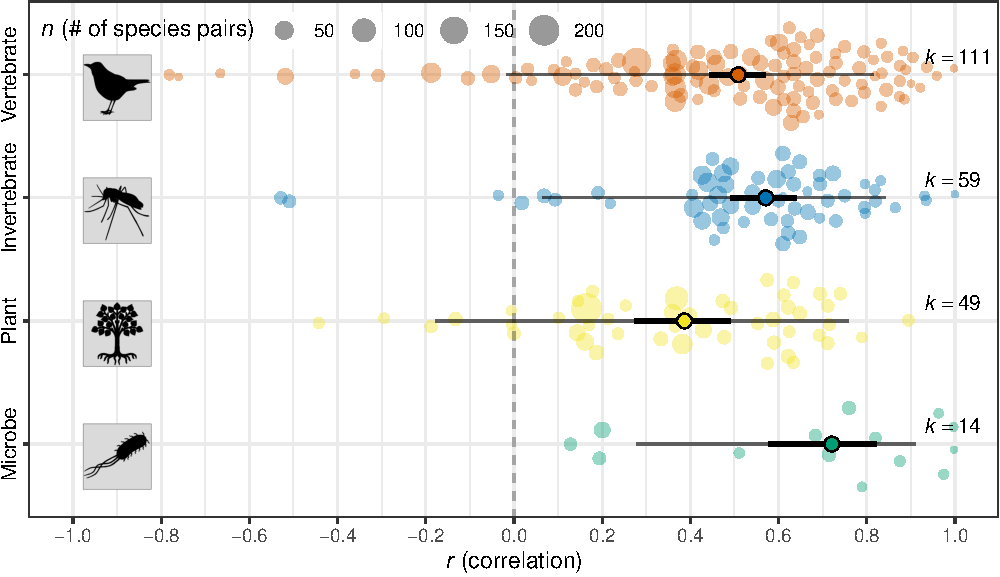
\includegraphics{Supporting_Information_files/figure-latex/unnamed-chunk-19-1.pdf}

\begin{Shaded}
\begin{Highlighting}[]
\CommentTok{# fig 3c}
\NormalTok{c <-}\StringTok{ }\KeywordTok{ggplot}\NormalTok{(}\DataTypeTok{data =}\NormalTok{ res_host_tax_broad1, }\KeywordTok{aes}\NormalTok{(}\DataTypeTok{x =} \KeywordTok{tanh}\NormalTok{(estimate), }\DataTypeTok{y =}\NormalTok{ name)) }\OperatorTok{+}
\StringTok{  }\KeywordTok{scale_x_continuous}\NormalTok{(}\DataTypeTok{limits=}\KeywordTok{c}\NormalTok{(}\OperatorTok{-}\DecValTok{1}\NormalTok{, }\DecValTok{1}\NormalTok{), }\DataTypeTok{breaks =} \KeywordTok{seq}\NormalTok{(}\OperatorTok{-}\DecValTok{1}\NormalTok{, }\DecValTok{1}\NormalTok{, }\DataTypeTok{by =} \FloatTok{0.2}\NormalTok{) ) }\OperatorTok{+}
\StringTok{  }\KeywordTok{geom_quasirandom}\NormalTok{(}\DataTypeTok{data =}\NormalTok{ dat }\OperatorTok\StringTok{ }\KeywordTok{filter}\NormalTok{(}\OperatorTok{!}\KeywordTok{is.na}\NormalTok{(host_tax_broad)), }
                   \KeywordTok{aes}\NormalTok{(}\DataTypeTok{x=} \KeywordTok{tanh}\NormalTok{(Zr), }\DataTypeTok{y =}\NormalTok{ host_tax_broad, }\DataTypeTok{size =}\NormalTok{ ((}\DecValTok{1}\OperatorTok{/}\NormalTok{VZr) }\OperatorTok{+}\StringTok{ }\DecValTok{3}\NormalTok{), }\DataTypeTok{colour =}\NormalTok{ host_tax_broad), }\DataTypeTok{groupOnX =} \OtherTok{FALSE}\NormalTok{, }\DataTypeTok{alpha=}\FloatTok{0.4}\NormalTok{) }\OperatorTok{+}\StringTok{ }
\StringTok{  }\CommentTok{# 95 %precition interval (PI)}
\StringTok{  }\KeywordTok{geom_errorbarh}\NormalTok{(}\KeywordTok{aes}\NormalTok{(}\DataTypeTok{xmin =} \KeywordTok{tanh}\NormalTok{(lowerPR), }\DataTypeTok{xmax =} \KeywordTok{tanh}\NormalTok{(upperPR)),  }\DataTypeTok{height =} \DecValTok{0}\NormalTok{, }\DataTypeTok{show.legend =}\NormalTok{ F, }\DataTypeTok{size =} \FloatTok{0.5}\NormalTok{, }\DataTypeTok{alpha =} \FloatTok{0.6}\NormalTok{) }\OperatorTok{+}
\StringTok{  }\CommentTok{# 95 %CI}
\StringTok{  }\KeywordTok{geom_errorbarh}\NormalTok{(}\KeywordTok{aes}\NormalTok{(}\DataTypeTok{xmin =} \KeywordTok{tanh}\NormalTok{(lowerCL), }\DataTypeTok{xmax =} \KeywordTok{tanh}\NormalTok{(upperCL)),  }\DataTypeTok{height =} \DecValTok{0}\NormalTok{, }\DataTypeTok{show.legend =}\NormalTok{ F, }\DataTypeTok{size =} \FloatTok{1.2}\NormalTok{) }\OperatorTok{+}
\StringTok{  }\KeywordTok{geom_vline}\NormalTok{(}\DataTypeTok{xintercept =} \DecValTok{0}\NormalTok{, }\DataTypeTok{linetype =} \DecValTok{2}\NormalTok{, }\DataTypeTok{colour =} \StringTok{"black"}\NormalTok{, }\DataTypeTok{alpha =} \FloatTok{0.3}\NormalTok{) }\OperatorTok{+}
\StringTok{  }\CommentTok{# creating dots and different size (bee-swarm and bubbles)}
\StringTok{  }\KeywordTok{geom_point}\NormalTok{(}\KeywordTok{aes}\NormalTok{(}\DataTypeTok{fill =}\NormalTok{ name), }\DataTypeTok{size =} \DecValTok{3}\NormalTok{, }\DataTypeTok{shape =} \DecValTok{21}\NormalTok{) }\OperatorTok{+}\StringTok{ }\CommentTok{#}
\StringTok{  }\CommentTok{# setting colours}
\StringTok{  }\KeywordTok{scale_color_manual}\NormalTok{(}\DataTypeTok{values =} \KeywordTok{c}\NormalTok{(}\StringTok{"Microbe"}\NormalTok{ =}\StringTok{ "#009E73"}\NormalTok{,  }\StringTok{"Plant"}\NormalTok{ =}\StringTok{ "#F0E422"}\NormalTok{,  }\StringTok{"Invert"}\NormalTok{=}\StringTok{ "#0072B2"}\NormalTok{,  }\StringTok{"Vert"}\NormalTok{ =}\StringTok{ "#D55E00"}\NormalTok{)) }\OperatorTok{+}
\StringTok{  }\KeywordTok{scale_fill_manual}\NormalTok{(}\DataTypeTok{values =} \KeywordTok{c}\NormalTok{(}\StringTok{"Microbe"}\NormalTok{ =}\StringTok{ "#009E73"}\NormalTok{,  }\StringTok{"Plant"}\NormalTok{ =}\StringTok{ "#F0E422"}\NormalTok{,  }\StringTok{"Invert"}\NormalTok{=}\StringTok{ "#0072B2"}\NormalTok{,  }\StringTok{"Vert"}\NormalTok{ =}\StringTok{ "#D55E00"}\NormalTok{)) }\OperatorTok{+}
\StringTok{  }\KeywordTok{scale_y_discrete}\NormalTok{(}\DataTypeTok{labels =} \KeywordTok{c}\NormalTok{(}\StringTok{"Microbe"}\NormalTok{ =}\StringTok{ "Microbe"}\NormalTok{,  }\StringTok{"Plant"}\NormalTok{ =}\StringTok{ "Plant"}\NormalTok{,  }\StringTok{"Invert"}\NormalTok{=}\StringTok{ "Invertebrate"}\NormalTok{,  }\StringTok{"Vert"}\NormalTok{ =}\StringTok{ "Vertebrate"}\NormalTok{)) }\OperatorTok{+}
\StringTok{  }\KeywordTok{annotate}\NormalTok{(}\StringTok{'text'}\NormalTok{, }\DataTypeTok{x =} \FloatTok{0.93}\NormalTok{, }\DataTypeTok{y =} \DecValTok{1}\OperatorTok{:}\DecValTok{4} \OperatorTok{+}\StringTok{ }\FloatTok{0.15}\NormalTok{, }\DataTypeTok{label=} \KeywordTok{paste}\NormalTok{(}\StringTok{"italic(k)=="}\NormalTok{, res_host_tax_broad1}\OperatorTok{$}\NormalTok{n), }\DataTypeTok{parse=}\OtherTok{TRUE}\NormalTok{, }\DataTypeTok{hjust =} \StringTok{"left"}\NormalTok{, }\DataTypeTok{size=}\FloatTok{3.5}\NormalTok{) }\OperatorTok{+}
\StringTok{  }\KeywordTok{labs}\NormalTok{(}\DataTypeTok{x =} \StringTok{""}\NormalTok{, }\DataTypeTok{y =} \StringTok{""}\NormalTok{, }\DataTypeTok{size =} \KeywordTok{expression}\NormalTok{(}\KeywordTok{paste}\NormalTok{(}\KeywordTok{italic}\NormalTok{(n), }\StringTok{" (# of species pairs)"}\NormalTok{)) , }\DataTypeTok{tag =} \StringTok{"c"}\NormalTok{) }\OperatorTok{+}
\StringTok{  }\KeywordTok{guides}\NormalTok{(}\DataTypeTok{fill =} \StringTok{"none"}\NormalTok{, }\DataTypeTok{colour =} \StringTok{"none"}\NormalTok{) }\OperatorTok{+}
\StringTok{  }\KeywordTok{theme_bw}\NormalTok{() }\OperatorTok{+}
\StringTok{  }\KeywordTok{theme}\NormalTok{(}\DataTypeTok{legend.position=}\StringTok{"none"}\NormalTok{) }\OperatorTok{+}
\StringTok{  }\KeywordTok{theme}\NormalTok{(}\DataTypeTok{axis.text.y =} \KeywordTok{element_text}\NormalTok{(}\DataTypeTok{size =} \DecValTok{10}\NormalTok{, }\DataTypeTok{colour =}\StringTok{"black"}\NormalTok{,}\DataTypeTok{hjust =} \FloatTok{0.5}\NormalTok{, }\DataTypeTok{angle =} \DecValTok{90}\NormalTok{)) }\OperatorTok{+}
\StringTok{  }\CommentTok{# putting pictures in}
\StringTok{  }\KeywordTok{annotation_custom}\NormalTok{(}\KeywordTok{rasterGrob}\NormalTok{(image_microbe_host), }\DataTypeTok{xmin =} \DecValTok{-1}\NormalTok{, }\DataTypeTok{xmax =} \FloatTok{-0.8}\NormalTok{, }\DataTypeTok{ymin =} \FloatTok{0.6}\NormalTok{, }\DataTypeTok{ymax =} \FloatTok{1.2}\NormalTok{) }\OperatorTok{+}\StringTok{ }
\StringTok{  }\KeywordTok{annotation_custom}\NormalTok{(}\KeywordTok{rasterGrob}\NormalTok{(image_plant_host), }\DataTypeTok{xmin =} \DecValTok{-1}\NormalTok{, }\DataTypeTok{xmax =} \FloatTok{-0.8}\NormalTok{, }\DataTypeTok{ymin =} \FloatTok{1.6}\NormalTok{, }\DataTypeTok{ymax =} \FloatTok{2.2}\NormalTok{) }\OperatorTok{+}
\StringTok{  }\KeywordTok{annotation_custom}\NormalTok{(}\KeywordTok{rasterGrob}\NormalTok{(image_invertebrate_host), }\DataTypeTok{xmin =} \DecValTok{-1}\NormalTok{, }\DataTypeTok{xmax =} \FloatTok{-0.8}\NormalTok{, }\DataTypeTok{ymin =} \FloatTok{2.6}\NormalTok{, }\DataTypeTok{ymax =} \FloatTok{3.2}\NormalTok{) }\OperatorTok{+}\StringTok{ }
\StringTok{  }\KeywordTok{annotation_custom}\NormalTok{(}\KeywordTok{rasterGrob}\NormalTok{(image_vertebrate_host), }\DataTypeTok{xmin =} \DecValTok{-1}\NormalTok{, }\DataTypeTok{xmax =} \FloatTok{-0.8}\NormalTok{, }\DataTypeTok{ymin =} \FloatTok{3.6}\NormalTok{, }\DataTypeTok{ymax =} \FloatTok{4.2}\NormalTok{)}
\end{Highlighting}
\end{Shaded}

\textbf{Figure 3c:} A forest plot showing the group-wise means (the
categorical variable \texttt{host\_tax\_broad}) with their 95\%
confidence intervals (thick lines) and 95\% prediction intervals (thin
lines), with observed effect sizes based on various sample sizes.

\hypertarget{the-effect-of-symbiont-taxa}{%
\paragraph{The effect of symbiont
taxa}\label{the-effect-of-symbiont-taxa}}

\begin{Shaded}
\begin{Highlighting}[]
\CommentTok{# reordering}
\NormalTok{dat}\OperatorTok{$}\NormalTok{symbiont_tax_broad <-}\StringTok{ }\KeywordTok{factor}\NormalTok{(dat}\OperatorTok{$}\NormalTok{symbiont_tax_broad, }\DataTypeTok{levels =} \KeywordTok{c}\NormalTok{(}\StringTok{"Microbe"}\NormalTok{, }\StringTok{"Plant"}\NormalTok{, }
    \StringTok{"Invert"}\NormalTok{, }\StringTok{"Vert"}\NormalTok{))}

\CommentTok{# sizes <- factor(sizes, levels = c('small', 'medium', 'large')) sizes > [1]}
\CommentTok{# small large large small medium > Levels: small medium large meta-regression:}
\CommentTok{# mutiple intercepts}
\NormalTok{mr_symbiont_tax_broad1 <-}\StringTok{ }\KeywordTok{rma.mv}\NormalTok{(}\DataTypeTok{yi =}\NormalTok{ Zr, }\DataTypeTok{V =}\NormalTok{ VZr, }\DataTypeTok{mods =} \OperatorTok{~}\NormalTok{symbiont_tax_broad }\OperatorTok{-}\StringTok{ }\DecValTok{1}\NormalTok{, }
    \DataTypeTok{test =} \StringTok{"t"}\NormalTok{, }\DataTypeTok{random =} \OperatorTok{~}\DecValTok{1} \OperatorTok{|}\StringTok{ }\NormalTok{authors, }\DataTypeTok{data =}\NormalTok{ dat)}

\CommentTok{# meta-regression: contrast 1}
\NormalTok{mr_symbiont_tax_broad2 <-}\StringTok{ }\KeywordTok{rma.mv}\NormalTok{(}\DataTypeTok{yi =}\NormalTok{ Zr, }\DataTypeTok{V =}\NormalTok{ VZr, }\DataTypeTok{mods =} \OperatorTok{~}\NormalTok{symbiont_tax_broad, }\DataTypeTok{test =} \StringTok{"t"}\NormalTok{, }
    \DataTypeTok{random =} \OperatorTok{~}\DecValTok{1} \OperatorTok{|}\StringTok{ }\NormalTok{authors, }\DataTypeTok{data =}\NormalTok{ dat)}

\CommentTok{# meta-regression: contrast 2}
\NormalTok{mr_symbiont_tax_broad3 <-}\StringTok{ }\KeywordTok{rma.mv}\NormalTok{(}\DataTypeTok{yi =}\NormalTok{ Zr, }\DataTypeTok{V =}\NormalTok{ VZr, }\DataTypeTok{mods =} \OperatorTok{~}\KeywordTok{relevel}\NormalTok{(symbiont_tax_broad, }
    \DataTypeTok{ref =} \StringTok{"Plant"}\NormalTok{), }\DataTypeTok{test =} \StringTok{"t"}\NormalTok{, }\DataTypeTok{random =} \OperatorTok{~}\DecValTok{1} \OperatorTok{|}\StringTok{ }\NormalTok{authors, }\DataTypeTok{data =}\NormalTok{ dat)}

\CommentTok{# meta-regression: contrast 3}
\NormalTok{mr_symbiont_tax_broad4 <-}\StringTok{ }\KeywordTok{rma.mv}\NormalTok{(}\DataTypeTok{yi =}\NormalTok{ Zr, }\DataTypeTok{V =}\NormalTok{ VZr, }\DataTypeTok{mods =} \OperatorTok{~}\KeywordTok{relevel}\NormalTok{(symbiont_tax_broad, }
    \DataTypeTok{ref =} \StringTok{"Invert"}\NormalTok{), }\DataTypeTok{test =} \StringTok{"t"}\NormalTok{, }\DataTypeTok{random =} \OperatorTok{~}\DecValTok{1} \OperatorTok{|}\StringTok{ }\NormalTok{authors, }\DataTypeTok{data =}\NormalTok{ dat)}
\end{Highlighting}
\end{Shaded}

\textbf{Supplementary Table 4:} Regression coefficients (Estimate), 95\%
confidence intervals (CIs), variance components (V) and variance
explained, \emph{R}\textsuperscript{2}\textsubscript{{[}marginal{]}}
(R2) from the meta-regression with \texttt{symbiont\_tax\_broad}.

\begin{Shaded}
\begin{Highlighting}[]
\CommentTok{# getting marginal R2}
\NormalTok{r2_symbiont_tax_broad1 <-}\StringTok{ }\KeywordTok{R2}\NormalTok{(mr_symbiont_tax_broad1)}

\CommentTok{# getting estimates}
\NormalTok{res_symbiont_tax_broad1 <-}\StringTok{ }\KeywordTok{get_est}\NormalTok{(mr_symbiont_tax_broad1, }\DataTypeTok{mod =} \StringTok{"symbiont_tax_broad"}\NormalTok{)}
\NormalTok{res_symbiont_tax_broad2 <-}\StringTok{ }\KeywordTok{get_est}\NormalTok{(mr_symbiont_tax_broad2, }\DataTypeTok{mod =} \StringTok{"symbiont_tax_broad"}\NormalTok{)}
\NormalTok{res_symbiont_tax_broad3 <-}\StringTok{ }\KeywordTok{get_est}\NormalTok{(mr_symbiont_tax_broad3, }\DataTypeTok{mod =} \StringTok{"symbiont_tax_broad"}\NormalTok{)}
\NormalTok{res_symbiont_tax_broad4 <-}\StringTok{ }\KeywordTok{get_est}\NormalTok{(mr_symbiont_tax_broad4, }\DataTypeTok{mod =} \StringTok{"symbiont_tax_broad"}\NormalTok{)}

\CommentTok{# creating a table}
\KeywordTok{tibble}\NormalTok{(}\StringTok{`}\DataTypeTok{Fixed effect}\StringTok{`}\NormalTok{ =}\StringTok{ }\KeywordTok{c}\NormalTok{(}\KeywordTok{as.character}\NormalTok{(res_symbiont_tax_broad1}\OperatorTok{$}\NormalTok{name), }\KeywordTok{cont_gen}\NormalTok{(res_symbiont_tax_broad1}\OperatorTok{$}\NormalTok{name)), }
    \DataTypeTok{Estimate =} \KeywordTok{c}\NormalTok{(res_symbiont_tax_broad1}\OperatorTok{$}\NormalTok{estimate, res_symbiont_tax_broad2}\OperatorTok{$}\NormalTok{estimate[}\OperatorTok{-}\DecValTok{1}\NormalTok{], }
\NormalTok{        res_symbiont_tax_broad3}\OperatorTok{$}\NormalTok{estimate[}\OperatorTok{-}\NormalTok{(}\DecValTok{1}\OperatorTok{:}\DecValTok{2}\NormalTok{)], res_symbiont_tax_broad4}\OperatorTok{$}\NormalTok{estimate[}\OperatorTok{-}\NormalTok{(}\DecValTok{1}\OperatorTok{:}\DecValTok{3}\NormalTok{)]), }
    \StringTok{`}\DataTypeTok{Lower CI [0.025]}\StringTok{`}\NormalTok{ =}\StringTok{ }\KeywordTok{c}\NormalTok{(res_symbiont_tax_broad1}\OperatorTok{$}\NormalTok{lowerCL, res_symbiont_tax_broad2}\OperatorTok{$}\NormalTok{lowerCL[}\OperatorTok{-}\DecValTok{1}\NormalTok{], }
\NormalTok{        res_symbiont_tax_broad3}\OperatorTok{$}\NormalTok{lowerCL[}\OperatorTok{-}\NormalTok{(}\DecValTok{1}\OperatorTok{:}\DecValTok{2}\NormalTok{)], res_symbiont_tax_broad4}\OperatorTok{$}\NormalTok{lowerCL[}\OperatorTok{-}\NormalTok{(}\DecValTok{1}\OperatorTok{:}\DecValTok{3}\NormalTok{)]), }
    \StringTok{`}\DataTypeTok{Upper CI  [0.975]}\StringTok{`}\NormalTok{ =}\StringTok{ }\KeywordTok{c}\NormalTok{(res_symbiont_tax_broad1}\OperatorTok{$}\NormalTok{upperCL, res_symbiont_tax_broad2}\OperatorTok{$}\NormalTok{upperCL[}\OperatorTok{-}\DecValTok{1}\NormalTok{], }
\NormalTok{        res_symbiont_tax_broad3}\OperatorTok{$}\NormalTok{upperCL[}\OperatorTok{-}\NormalTok{(}\DecValTok{1}\OperatorTok{:}\DecValTok{2}\NormalTok{)], res_symbiont_tax_broad4}\OperatorTok{$}\NormalTok{upperCL[}\OperatorTok{-}\NormalTok{(}\DecValTok{1}\OperatorTok{:}\DecValTok{3}\NormalTok{)]), }
    \StringTok{`}\DataTypeTok{V[authors]}\StringTok{`}\NormalTok{ =}\StringTok{ }\KeywordTok{c}\NormalTok{(mr_symbiont_tax_broad1}\OperatorTok{$}\NormalTok{sigma2, }\KeywordTok{rep}\NormalTok{(}\OtherTok{NA}\NormalTok{, }\DecValTok{9}\NormalTok{)), }\DataTypeTok{R2 =} \KeywordTok{c}\NormalTok{(r2_symbiont_tax_broad1[}\DecValTok{1}\NormalTok{], }
        \KeywordTok{rep}\NormalTok{(}\OtherTok{NA}\NormalTok{, }\DecValTok{9}\NormalTok{))) }\OperatorTok\StringTok{ }\KeywordTok{kable}\NormalTok{(}\StringTok{"html"}\NormalTok{, }\DataTypeTok{digits =} \DecValTok{3}\NormalTok{) }\OperatorTok\StringTok{ }\KeywordTok{kable_styling}\NormalTok{(}\StringTok{"striped"}\NormalTok{, }\DataTypeTok{position =} \StringTok{"left"}\NormalTok{) }\OperatorTok\StringTok{ }
\StringTok{    }\KeywordTok{scroll_box}\NormalTok{(}\DataTypeTok{width =} \StringTok{"100%"}\NormalTok{, }\DataTypeTok{height =} \StringTok{"300px"}\NormalTok{)}
\end{Highlighting}
\end{Shaded}

Fixed effect

Estimate

Lower CI {[}0.025{]}

Upper CI {[}0.975{]}

V{[}authors{]}

R2

Microbe

0.576

0.494

0.658

0.087

0.073

Plant

1.188

0.703

1.674

NA

NA

Invert

0.549

0.460

0.639

NA

NA

Vert

0.496

-0.172

1.163

NA

NA

Microbe-Plant

0.613

0.120

1.105

NA

NA

Microbe-Invert

-0.027

-0.148

0.095

NA

NA

Microbe-Vert

-0.080

-0.753

0.592

NA

NA

Plant-Invert

-0.639

-1.133

-0.146

NA

NA

Plant-Vert

-0.693

-1.518

0.132

NA

NA

Invert-Vert

-0.054

-0.727

0.620

NA

NA

\begin{Shaded}
\begin{Highlighting}[]
\CommentTok{# getting images}
\NormalTok{image_invertebrate_parasite <-}\StringTok{ }\KeywordTok{readPNG}\NormalTok{(}\KeywordTok{here}\NormalTok{(}\StringTok{"images/invertebrate_parasite_transparentbg.png"}\NormalTok{))}
\NormalTok{image_microbe_parasite <-}\StringTok{ }\KeywordTok{readPNG}\NormalTok{(}\KeywordTok{here}\NormalTok{(}\StringTok{"images/microbe_parasite_transparentbg.png"}\NormalTok{))}
\NormalTok{image_vertebrate_parasite <-}\StringTok{ }\KeywordTok{readPNG}\NormalTok{(}\KeywordTok{here}\NormalTok{(}\StringTok{"images/vertebrate_parasite_transparentbg.png"}\NormalTok{))}
\NormalTok{image_plant_parasite <-}\StringTok{ }\KeywordTok{readPNG}\NormalTok{(}\KeywordTok{here}\NormalTok{(}\StringTok{"images/plant_parasite_transparentbg.png"}\NormalTok{))}

\CommentTok{# adding sample size (k) for each category}
\NormalTok{k_symbiont_tax_broad <-}\StringTok{ }\NormalTok{dat }\OperatorTok\StringTok{ }\KeywordTok{group_by}\NormalTok{(symbiont_tax_broad) }\OperatorTok\StringTok{ }\KeywordTok{count}\NormalTok{()}
\CommentTok{# getting estimates and predicitons}
\NormalTok{pred_symbiont_tax_broad <-}\StringTok{ }\KeywordTok{get_pred}\NormalTok{(mr_symbiont_tax_broad1, }\DataTypeTok{mod =} \StringTok{"symbiont_tax_broad"}\NormalTok{) }
\NormalTok{res_symbiont_tax_broad1 <-}\StringTok{ }\KeywordTok{left_join}\NormalTok{(res_symbiont_tax_broad1, k_symbiont_tax_broad, }\DataTypeTok{by =}  \KeywordTok{c}\NormalTok{(}\StringTok{"name"}\NormalTok{ =}\StringTok{ "symbiont_tax_broad"}\NormalTok{))  }\OperatorTok\StringTok{ }\KeywordTok{left_join}\NormalTok{(pred_symbiont_tax_broad)}
\CommentTok{#res_symbiosis1 }
\CommentTok{# drawing a funnel plot - fig 2b}
\NormalTok{fig_symbiont_tax_broad <-}\StringTok{ }\KeywordTok{ggplot}\NormalTok{(}\DataTypeTok{data =}\NormalTok{ res_symbiont_tax_broad1, }\KeywordTok{aes}\NormalTok{(}\DataTypeTok{x =} \KeywordTok{tanh}\NormalTok{(estimate), }\DataTypeTok{y =}\NormalTok{ name)) }\OperatorTok{+}
\StringTok{  }\KeywordTok{scale_x_continuous}\NormalTok{(}\DataTypeTok{limits=}\KeywordTok{c}\NormalTok{(}\OperatorTok{-}\DecValTok{1}\NormalTok{, }\DecValTok{1}\NormalTok{), }\DataTypeTok{breaks =} \KeywordTok{seq}\NormalTok{(}\OperatorTok{-}\DecValTok{1}\NormalTok{, }\DecValTok{1}\NormalTok{, }\DataTypeTok{by =} \FloatTok{0.2}\NormalTok{) ) }\OperatorTok{+}
\StringTok{  }\KeywordTok{geom_quasirandom}\NormalTok{(}\DataTypeTok{data =}\NormalTok{ dat }\OperatorTok\StringTok{ }\KeywordTok{filter}\NormalTok{(}\OperatorTok{!}\KeywordTok{is.na}\NormalTok{(symbiont_tax_broad)), }
                   \KeywordTok{aes}\NormalTok{(}\DataTypeTok{x=} \KeywordTok{tanh}\NormalTok{(Zr), }\DataTypeTok{y =}\NormalTok{ symbiont_tax_broad, }\DataTypeTok{size =}\NormalTok{ ((}\DecValTok{1}\OperatorTok{/}\NormalTok{VZr) }\OperatorTok{+}\StringTok{ }\DecValTok{3}\NormalTok{), }\DataTypeTok{colour =}\NormalTok{ symbiont_tax_broad), }\DataTypeTok{groupOnX =} \OtherTok{FALSE}\NormalTok{, }\DataTypeTok{alpha=}\FloatTok{0.4}\NormalTok{) }\OperatorTok{+}\StringTok{ }
\StringTok{  }\CommentTok{# 95 %precition interval (PI)}
\StringTok{  }\KeywordTok{geom_errorbarh}\NormalTok{(}\KeywordTok{aes}\NormalTok{(}\DataTypeTok{xmin =} \KeywordTok{tanh}\NormalTok{(lowerPR), }\DataTypeTok{xmax =} \KeywordTok{tanh}\NormalTok{(upperPR)),  }\DataTypeTok{height =} \DecValTok{0}\NormalTok{, }\DataTypeTok{show.legend =}\NormalTok{ F, }\DataTypeTok{size =} \FloatTok{0.5}\NormalTok{, }\DataTypeTok{alpha =} \FloatTok{0.6}\NormalTok{) }\OperatorTok{+}
\StringTok{  }\CommentTok{# 95 %CI}
\StringTok{  }\KeywordTok{geom_errorbarh}\NormalTok{(}\KeywordTok{aes}\NormalTok{(}\DataTypeTok{xmin =} \KeywordTok{tanh}\NormalTok{(lowerCL), }\DataTypeTok{xmax =} \KeywordTok{tanh}\NormalTok{(upperCL)),  }\DataTypeTok{height =} \DecValTok{0}\NormalTok{, }\DataTypeTok{show.legend =}\NormalTok{ F, }\DataTypeTok{size =} \FloatTok{1.2}\NormalTok{) }\OperatorTok{+}
\StringTok{  }\KeywordTok{geom_vline}\NormalTok{(}\DataTypeTok{xintercept =} \DecValTok{0}\NormalTok{, }\DataTypeTok{linetype =} \DecValTok{2}\NormalTok{, }\DataTypeTok{colour =} \StringTok{"black"}\NormalTok{, }\DataTypeTok{alpha =} \FloatTok{0.3}\NormalTok{) }\OperatorTok{+}
\StringTok{  }\CommentTok{# creating dots and different size (bee-swarm and bubbles)}
\StringTok{  }\KeywordTok{geom_point}\NormalTok{(}\KeywordTok{aes}\NormalTok{(}\DataTypeTok{fill =}\NormalTok{ name), }\DataTypeTok{size =} \DecValTok{3}\NormalTok{, }\DataTypeTok{shape =} \DecValTok{21}\NormalTok{) }\OperatorTok{+}\StringTok{ }\CommentTok{#}
\StringTok{  }\CommentTok{# setting colours}
\StringTok{  }\KeywordTok{scale_color_manual}\NormalTok{(}\DataTypeTok{values =} \KeywordTok{c}\NormalTok{(}\StringTok{"Microbe"}\NormalTok{ =}\StringTok{ "#009E73"}\NormalTok{,  }\StringTok{"Plant"}\NormalTok{ =}\StringTok{ "#F0E422"}\NormalTok{,  }\StringTok{"Invert"}\NormalTok{=}\StringTok{ "#0072B2"}\NormalTok{,  }\StringTok{"Vert"}\NormalTok{ =}\StringTok{ "#D55E00"}\NormalTok{ )) }\OperatorTok{+}
\StringTok{  }\KeywordTok{scale_fill_manual}\NormalTok{(}\DataTypeTok{values =} \KeywordTok{c}\NormalTok{(}\StringTok{"Microbe"}\NormalTok{ =}\StringTok{ "#009E73"}\NormalTok{,  }\StringTok{"Plant"}\NormalTok{ =}\StringTok{ "#F0E422"}\NormalTok{,  }\StringTok{"Invert"}\NormalTok{=}\StringTok{ "#0072B2"}\NormalTok{,  }\StringTok{"Vert"}\NormalTok{ =}\StringTok{ "#D55E00"}\NormalTok{)) }\OperatorTok{+}
\StringTok{  }\KeywordTok{scale_y_discrete}\NormalTok{(}\DataTypeTok{labels =} \KeywordTok{c}\NormalTok{(}\StringTok{"Microbe"}\NormalTok{ =}\StringTok{ "Microbe"}\NormalTok{,  }\StringTok{"Plant"}\NormalTok{ =}\StringTok{ "Plant"}\NormalTok{,  }\StringTok{"Invert"}\NormalTok{=}\StringTok{ "Invertebrate"}\NormalTok{,  }\StringTok{"Vert"}\NormalTok{ =}\StringTok{ "Vertebrate"}\NormalTok{)) }\OperatorTok{+}
\StringTok{  }\KeywordTok{annotate}\NormalTok{(}\StringTok{'text'}\NormalTok{, }\DataTypeTok{x =} \FloatTok{0.93}\NormalTok{, }\DataTypeTok{y =} \DecValTok{1}\OperatorTok{:}\DecValTok{4} \OperatorTok{+}\StringTok{ }\FloatTok{0.15}\NormalTok{, }\DataTypeTok{label=} \KeywordTok{paste}\NormalTok{(}\StringTok{"italic(k)=="}\NormalTok{, res_symbiont_tax_broad1}\OperatorTok{$}\NormalTok{n), }\DataTypeTok{parse=}\OtherTok{TRUE}\NormalTok{, }\DataTypeTok{hjust =} \StringTok{"left"}\NormalTok{, }\DataTypeTok{size=}\FloatTok{3.5}\NormalTok{) }\OperatorTok{+}
\StringTok{  }\KeywordTok{labs}\NormalTok{(}\DataTypeTok{x =} \KeywordTok{expression}\NormalTok{(}\KeywordTok{paste}\NormalTok{(}\KeywordTok{italic}\NormalTok{(r), }\StringTok{" (correlation)"}\NormalTok{)), }\DataTypeTok{y =} \StringTok{""}\NormalTok{, }\DataTypeTok{size =} \KeywordTok{expression}\NormalTok{(}\KeywordTok{paste}\NormalTok{(}\KeywordTok{italic}\NormalTok{(n), }\StringTok{" (# of species pairs)"}\NormalTok{)) ) }\OperatorTok{+}
\StringTok{  }\KeywordTok{guides}\NormalTok{(}\DataTypeTok{fill =} \StringTok{"none"}\NormalTok{, }\DataTypeTok{colour =} \StringTok{"none"}\NormalTok{) }\OperatorTok{+}
\StringTok{  }\KeywordTok{theme_bw}\NormalTok{() }\OperatorTok{+}
\StringTok{  }\KeywordTok{theme}\NormalTok{(}\DataTypeTok{legend.position=} \KeywordTok{c}\NormalTok{(}\DecValTok{0}\NormalTok{, }\DecValTok{1}\NormalTok{), }\DataTypeTok{legend.justification =} \KeywordTok{c}\NormalTok{(}\DecValTok{0}\NormalTok{,}\DecValTok{1}\NormalTok{)) }\OperatorTok{+}
\StringTok{  }\KeywordTok{theme}\NormalTok{(}\DataTypeTok{legend.direction=}\StringTok{"horizontal"}\NormalTok{) }\OperatorTok{+}
\StringTok{  }\CommentTok{#theme(legend.background = element_rect(fill = "white", colour = "black")) +}
\StringTok{  }\KeywordTok{theme}\NormalTok{(}\DataTypeTok{legend.background =} \KeywordTok{element_blank}\NormalTok{()) }\OperatorTok{+}
\StringTok{  }\KeywordTok{theme}\NormalTok{(}\DataTypeTok{axis.text.y =} \KeywordTok{element_text}\NormalTok{(}\DataTypeTok{size =} \DecValTok{10}\NormalTok{, }\DataTypeTok{colour =}\StringTok{"black"}\NormalTok{, }\DataTypeTok{hjust =} \FloatTok{0.5}\NormalTok{, }\DataTypeTok{angle =} \DecValTok{90}\NormalTok{)) }\OperatorTok{+}
\StringTok{  }\CommentTok{# putting pictures in}
\StringTok{  }\KeywordTok{annotation_custom}\NormalTok{(}\KeywordTok{rasterGrob}\NormalTok{(image_microbe_parasite), }\DataTypeTok{xmin =} \DecValTok{-1}\NormalTok{, }\DataTypeTok{xmax =} \FloatTok{-0.8}\NormalTok{, }\DataTypeTok{ymin =} \FloatTok{0.6}\NormalTok{, }\DataTypeTok{ymax =} \FloatTok{1.2}\NormalTok{) }\OperatorTok{+}\StringTok{ }
\StringTok{  }\KeywordTok{annotation_custom}\NormalTok{(}\KeywordTok{rasterGrob}\NormalTok{(image_plant_parasite), }\DataTypeTok{xmin =} \DecValTok{-1}\NormalTok{, }\DataTypeTok{xmax =} \FloatTok{-0.8}\NormalTok{, }\DataTypeTok{ymin =} \FloatTok{1.6}\NormalTok{, }\DataTypeTok{ymax =} \FloatTok{2.2}\NormalTok{) }\OperatorTok{+}
\StringTok{  }\KeywordTok{annotation_custom}\NormalTok{(}\KeywordTok{rasterGrob}\NormalTok{(image_invertebrate_parasite), }\DataTypeTok{xmin =} \DecValTok{-1}\NormalTok{, }\DataTypeTok{xmax =} \FloatTok{-0.8}\NormalTok{, }\DataTypeTok{ymin =} \FloatTok{2.6}\NormalTok{, }\DataTypeTok{ymax =} \FloatTok{3.2}\NormalTok{) }\OperatorTok{+}\StringTok{ }
\StringTok{  }\KeywordTok{annotation_custom}\NormalTok{(}\KeywordTok{rasterGrob}\NormalTok{(image_vertebrate_parasite), }\DataTypeTok{xmin =} \DecValTok{-1}\NormalTok{, }\DataTypeTok{xmax =} \FloatTok{-0.8}\NormalTok{, }\DataTypeTok{ymin =} \FloatTok{3.6}\NormalTok{, }\DataTypeTok{ymax =} \FloatTok{4.2}\NormalTok{)}

\NormalTok{fig_symbiont_tax_broad}
\end{Highlighting}
\end{Shaded}

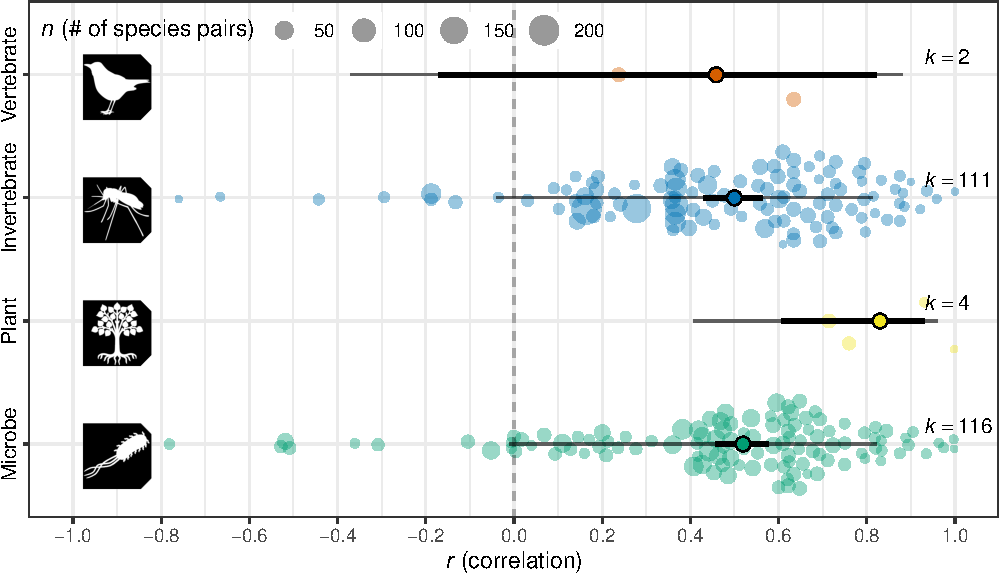
\includegraphics{Supporting_Information_files/figure-latex/unnamed-chunk-22-1.pdf}

\begin{Shaded}
\begin{Highlighting}[]
\CommentTok{# fig 3d}
\NormalTok{d <-}\StringTok{ }\KeywordTok{ggplot}\NormalTok{(}\DataTypeTok{data =}\NormalTok{ res_symbiont_tax_broad1, }\KeywordTok{aes}\NormalTok{(}\DataTypeTok{x =} \KeywordTok{tanh}\NormalTok{(estimate), }\DataTypeTok{y =}\NormalTok{ name)) }\OperatorTok{+}
\StringTok{  }\KeywordTok{scale_x_continuous}\NormalTok{(}\DataTypeTok{limits=}\KeywordTok{c}\NormalTok{(}\OperatorTok{-}\DecValTok{1}\NormalTok{, }\DecValTok{1}\NormalTok{), }\DataTypeTok{breaks =} \KeywordTok{seq}\NormalTok{(}\OperatorTok{-}\DecValTok{1}\NormalTok{, }\DecValTok{1}\NormalTok{, }\DataTypeTok{by =} \FloatTok{0.2}\NormalTok{) ) }\OperatorTok{+}
\StringTok{  }\KeywordTok{geom_quasirandom}\NormalTok{(}\DataTypeTok{data =}\NormalTok{ dat }\OperatorTok\StringTok{ }\KeywordTok{filter}\NormalTok{(}\OperatorTok{!}\KeywordTok{is.na}\NormalTok{(symbiont_tax_broad)), }
                   \KeywordTok{aes}\NormalTok{(}\DataTypeTok{x=} \KeywordTok{tanh}\NormalTok{(Zr), }\DataTypeTok{y =}\NormalTok{ symbiont_tax_broad, }\DataTypeTok{size =}\NormalTok{ ((}\DecValTok{1}\OperatorTok{/}\NormalTok{VZr) }\OperatorTok{+}\StringTok{ }\DecValTok{3}\NormalTok{), }\DataTypeTok{colour =}\NormalTok{ symbiont_tax_broad), }\DataTypeTok{groupOnX =} \OtherTok{FALSE}\NormalTok{, }\DataTypeTok{alpha=}\FloatTok{0.4}\NormalTok{) }\OperatorTok{+}\StringTok{ }
\StringTok{  }\CommentTok{# 95 %precition interval (PI)}
\StringTok{  }\KeywordTok{geom_errorbarh}\NormalTok{(}\KeywordTok{aes}\NormalTok{(}\DataTypeTok{xmin =} \KeywordTok{tanh}\NormalTok{(lowerPR), }\DataTypeTok{xmax =} \KeywordTok{tanh}\NormalTok{(upperPR)),  }\DataTypeTok{height =} \DecValTok{0}\NormalTok{, }\DataTypeTok{show.legend =}\NormalTok{ F, }\DataTypeTok{size =} \FloatTok{0.5}\NormalTok{, }\DataTypeTok{alpha =} \FloatTok{0.6}\NormalTok{) }\OperatorTok{+}
\StringTok{  }\CommentTok{# 95 %CI}
\StringTok{  }\KeywordTok{geom_errorbarh}\NormalTok{(}\KeywordTok{aes}\NormalTok{(}\DataTypeTok{xmin =} \KeywordTok{tanh}\NormalTok{(lowerCL), }\DataTypeTok{xmax =} \KeywordTok{tanh}\NormalTok{(upperCL)),  }\DataTypeTok{height =} \DecValTok{0}\NormalTok{, }\DataTypeTok{show.legend =}\NormalTok{ F, }\DataTypeTok{size =} \FloatTok{1.2}\NormalTok{) }\OperatorTok{+}
\StringTok{  }\KeywordTok{geom_vline}\NormalTok{(}\DataTypeTok{xintercept =} \DecValTok{0}\NormalTok{, }\DataTypeTok{linetype =} \DecValTok{2}\NormalTok{, }\DataTypeTok{colour =} \StringTok{"black"}\NormalTok{, }\DataTypeTok{alpha =} \FloatTok{0.3}\NormalTok{) }\OperatorTok{+}
\StringTok{  }\CommentTok{# creating dots and different size (bee-swarm and bubbles)}
\StringTok{  }\KeywordTok{geom_point}\NormalTok{(}\KeywordTok{aes}\NormalTok{(}\DataTypeTok{fill =}\NormalTok{ name), }\DataTypeTok{size =} \DecValTok{3}\NormalTok{, }\DataTypeTok{shape =} \DecValTok{21}\NormalTok{) }\OperatorTok{+}\StringTok{ }\CommentTok{#}
\StringTok{  }\CommentTok{# setting colours}
\StringTok{  }\KeywordTok{scale_color_manual}\NormalTok{(}\DataTypeTok{values =} \KeywordTok{c}\NormalTok{(}\StringTok{"Microbe"}\NormalTok{ =}\StringTok{ "#009E73"}\NormalTok{,  }\StringTok{"Plant"}\NormalTok{ =}\StringTok{ "#F0E422"}\NormalTok{,  }\StringTok{"Invert"}\NormalTok{=}\StringTok{ "#0072B2"}\NormalTok{,  }\StringTok{"Vert"}\NormalTok{ =}\StringTok{ "#D55E00"}\NormalTok{ )) }\OperatorTok{+}
\StringTok{  }\KeywordTok{scale_fill_manual}\NormalTok{(}\DataTypeTok{values =} \KeywordTok{c}\NormalTok{(}\StringTok{"Microbe"}\NormalTok{ =}\StringTok{ "#009E73"}\NormalTok{,  }\StringTok{"Plant"}\NormalTok{ =}\StringTok{ "#F0E422"}\NormalTok{,  }\StringTok{"Invert"}\NormalTok{=}\StringTok{ "#0072B2"}\NormalTok{,  }\StringTok{"Vert"}\NormalTok{ =}\StringTok{ "#D55E00"}\NormalTok{)) }\OperatorTok{+}
\StringTok{  }\KeywordTok{scale_y_discrete}\NormalTok{(}\DataTypeTok{labels =} \KeywordTok{c}\NormalTok{(}\StringTok{"Microbe"}\NormalTok{ =}\StringTok{ "Microbe"}\NormalTok{,  }\StringTok{"Plant"}\NormalTok{ =}\StringTok{ "Plant"}\NormalTok{,  }\StringTok{"Invert"}\NormalTok{=}\StringTok{ "Invertebrate"}\NormalTok{,  }\StringTok{"Vert"}\NormalTok{ =}\StringTok{ "Vertebrate"}\NormalTok{)) }\OperatorTok{+}
\StringTok{  }\KeywordTok{annotate}\NormalTok{(}\StringTok{'text'}\NormalTok{, }\DataTypeTok{x =} \FloatTok{0.93}\NormalTok{, }\DataTypeTok{y =} \DecValTok{1}\OperatorTok{:}\DecValTok{4} \OperatorTok{+}\StringTok{ }\FloatTok{0.15}\NormalTok{, }\DataTypeTok{label=} \KeywordTok{paste}\NormalTok{(}\StringTok{"italic(k)=="}\NormalTok{, res_symbiont_tax_broad1}\OperatorTok{$}\NormalTok{n), }\DataTypeTok{parse=}\OtherTok{TRUE}\NormalTok{, }\DataTypeTok{hjust =} \StringTok{"left"}\NormalTok{, }\DataTypeTok{size=}\FloatTok{3.5}\NormalTok{) }\OperatorTok{+}
\StringTok{  }\KeywordTok{labs}\NormalTok{(}\DataTypeTok{x =} \KeywordTok{expression}\NormalTok{(}\KeywordTok{paste}\NormalTok{(}\KeywordTok{italic}\NormalTok{(r), }\StringTok{" (correlation)"}\NormalTok{)), }\DataTypeTok{y =} \StringTok{""}\NormalTok{, }\DataTypeTok{size =} \KeywordTok{expression}\NormalTok{(}\KeywordTok{paste}\NormalTok{(}\KeywordTok{italic}\NormalTok{(n), }\StringTok{" (# of species pairs)"}\NormalTok{)), }\DataTypeTok{tag =} \StringTok{"d"}\NormalTok{) }\OperatorTok{+}
\StringTok{  }\KeywordTok{guides}\NormalTok{(}\DataTypeTok{fill =} \StringTok{"none"}\NormalTok{, }\DataTypeTok{colour =} \StringTok{"none"}\NormalTok{) }\OperatorTok{+}
\StringTok{  }\KeywordTok{theme_bw}\NormalTok{() }\OperatorTok{+}
\StringTok{  }\KeywordTok{theme}\NormalTok{(}\DataTypeTok{legend.position=}\StringTok{"none"}\NormalTok{) }\OperatorTok{+}
\StringTok{  }\KeywordTok{theme}\NormalTok{(}\DataTypeTok{axis.text.y =} \KeywordTok{element_text}\NormalTok{(}\DataTypeTok{size =} \DecValTok{10}\NormalTok{, }\DataTypeTok{colour =}\StringTok{"black"}\NormalTok{,}\DataTypeTok{hjust =} \FloatTok{0.5}\NormalTok{, }\DataTypeTok{angle =} \DecValTok{90}\NormalTok{)) }\OperatorTok{+}
\StringTok{  }\CommentTok{# putting pictures in}
\StringTok{  }\KeywordTok{annotation_custom}\NormalTok{(}\KeywordTok{rasterGrob}\NormalTok{(image_microbe_parasite), }\DataTypeTok{xmin =} \DecValTok{-1}\NormalTok{, }\DataTypeTok{xmax =} \FloatTok{-0.8}\NormalTok{, }\DataTypeTok{ymin =} \FloatTok{0.6}\NormalTok{, }\DataTypeTok{ymax =} \FloatTok{1.2}\NormalTok{) }\OperatorTok{+}\StringTok{ }
\StringTok{  }\KeywordTok{annotation_custom}\NormalTok{(}\KeywordTok{rasterGrob}\NormalTok{(image_plant_parasite), }\DataTypeTok{xmin =} \DecValTok{-1}\NormalTok{, }\DataTypeTok{xmax =} \FloatTok{-0.8}\NormalTok{, }\DataTypeTok{ymin =} \FloatTok{1.6}\NormalTok{, }\DataTypeTok{ymax =} \FloatTok{2.2}\NormalTok{) }\OperatorTok{+}
\StringTok{  }\KeywordTok{annotation_custom}\NormalTok{(}\KeywordTok{rasterGrob}\NormalTok{(image_invertebrate_parasite), }\DataTypeTok{xmin =} \DecValTok{-1}\NormalTok{, }\DataTypeTok{xmax =} \FloatTok{-0.8}\NormalTok{, }\DataTypeTok{ymin =} \FloatTok{2.6}\NormalTok{, }\DataTypeTok{ymax =} \FloatTok{3.2}\NormalTok{) }\OperatorTok{+}\StringTok{ }
\StringTok{  }\KeywordTok{annotation_custom}\NormalTok{(}\KeywordTok{rasterGrob}\NormalTok{(image_vertebrate_parasite), }\DataTypeTok{xmin =} \DecValTok{-1}\NormalTok{, }\DataTypeTok{xmax =} \FloatTok{-0.8}\NormalTok{, }\DataTypeTok{ymin =} \FloatTok{3.6}\NormalTok{, }\DataTypeTok{ymax =} \FloatTok{4.2}\NormalTok{)}
\end{Highlighting}
\end{Shaded}

\textbf{Figure 2d:} A forest plot showing the group-wise means (the
categorical variable \texttt{symbiont\_tax\_broad}) with their 95\%
confidence intervals (thick lines) and 95\% prediction intervals (thin
lines), with observed effect sizes based on various sample sizes.

\hypertarget{testing-specialization-1-host-range}{%
\paragraph{Testing specialization 1: host
range}\label{testing-specialization-1-host-range}}

\begin{Shaded}
\begin{Highlighting}[]
\CommentTok{# meta-regression}
\NormalTok{mr_host_range_link_ratio <-}\StringTok{ }\KeywordTok{rma.mv}\NormalTok{(}\DataTypeTok{yi =}\NormalTok{ Zr, }\DataTypeTok{V =}\NormalTok{ VZr, }\DataTypeTok{mods =} \OperatorTok{~}\KeywordTok{log}\NormalTok{(host_range_link_ratio), }
    \DataTypeTok{random =} \OperatorTok{~}\DecValTok{1} \OperatorTok{|}\StringTok{ }\NormalTok{authors, }\DataTypeTok{data =}\NormalTok{ dat)}
\end{Highlighting}
\end{Shaded}

\textbf{Supplementary Table 5:} Regression coefficients (Estimate), 95\%
confidence intervals (CIs), variance components (V) and variance
explained, \emph{R}\textsuperscript{2}\textsubscript{{[}marginal{]}}
(R2) from the meta-regression with
\texttt{log(host\_range\_link\_ratio)}.

\begin{Shaded}
\begin{Highlighting}[]
\CommentTok{# getting marginal R2}
\NormalTok{r2_host_range_link_ratio <-}\StringTok{ }\KeywordTok{R2}\NormalTok{(mr_host_range_link_ratio)}

\CommentTok{# getting estimates: name does not work for slopes}
\NormalTok{res_host_range_link_ratio <-}\StringTok{ }\KeywordTok{get_est}\NormalTok{(mr_host_range_link_ratio, }\DataTypeTok{mod =} \StringTok{"log(host_range_link_ratio)"}\NormalTok{)}

\CommentTok{# creating a table}
\KeywordTok{tibble}\NormalTok{(}\StringTok{`}\DataTypeTok{Fixed effect}\StringTok{`}\NormalTok{ =}\StringTok{ }\KeywordTok{c}\NormalTok{(}\StringTok{"Intercept"}\NormalTok{, }\StringTok{"log(host_range_link_ratio)"}\NormalTok{), }\DataTypeTok{Estimate =} \KeywordTok{c}\NormalTok{(res_host_range_link_ratio}\OperatorTok{$}\NormalTok{estimate), }
    \StringTok{`}\DataTypeTok{Lower CI [0.025]}\StringTok{`}\NormalTok{ =}\StringTok{ }\KeywordTok{c}\NormalTok{(res_host_range_link_ratio}\OperatorTok{$}\NormalTok{lowerCL), }\StringTok{`}\DataTypeTok{Upper CI  [0.975]}\StringTok{`}\NormalTok{ =}\StringTok{ }\KeywordTok{c}\NormalTok{(res_host_range_link_ratio}\OperatorTok{$}\NormalTok{upperCL), }
    \StringTok{`}\DataTypeTok{V[authors]}\StringTok{`}\NormalTok{ =}\StringTok{ }\KeywordTok{c}\NormalTok{(mr_host_range_link_ratio}\OperatorTok{$}\NormalTok{sigma2, }\OtherTok{NA}\NormalTok{), }\DataTypeTok{R2 =} \KeywordTok{c}\NormalTok{(r2_host_range_link_ratio[}\DecValTok{1}\NormalTok{], }
        \OtherTok{NA}\NormalTok{)) }\OperatorTok\StringTok{ }\KeywordTok{kable}\NormalTok{(}\StringTok{"html"}\NormalTok{, }\DataTypeTok{digits =} \DecValTok{3}\NormalTok{) }\OperatorTok\StringTok{ }\KeywordTok{kable_styling}\NormalTok{(}\StringTok{"striped"}\NormalTok{, }\DataTypeTok{position =} \StringTok{"left"}\NormalTok{)}
\end{Highlighting}
\end{Shaded}

Fixed effect

Estimate

Lower CI {[}0.025{]}

Upper CI {[}0.975{]}

V{[}authors{]}

R2

Intercept

0.577

0.509

0.645

0.09

0

log(host\_range\_link\_ratio)

0.009

-0.156

0.173

NA

NA

\begin{Shaded}
\begin{Highlighting}[]
\CommentTok{# newmods <- seq(-0.3, 2.2, by = 0.1)}
\CommentTok{# pred_host_range_link_ratio <-predict.rma(mr_host_range_link_ratio, newmods = newmods) }
\CommentTok{# ribbon_dat <- tibble(newmods = newmods, ymin = pred_host_range_link_ratio$ci.lb, ymax = pred_host_range_link_ratio$ci.ub)}
\NormalTok{pred_host_range_link_ratio <-}\KeywordTok{predict.rma}\NormalTok{(mr_host_range_link_ratio) }

\CommentTok{# plotting}

\NormalTok{fig_host_range_link_ratio <-}\StringTok{  }\NormalTok{dat }\OperatorTok\StringTok{ }
\StringTok{  }\KeywordTok{filter}\NormalTok{(}\OperatorTok{!}\KeywordTok{is.na}\NormalTok{(host_range_link_ratio))  }\OperatorTok\StringTok{ }\CommentTok{# getting ride of NA values}
\StringTok{  }\KeywordTok{mutate}\NormalTok{(}\DataTypeTok{ymin =}\NormalTok{ pred_host_range_link_ratio}\OperatorTok{$}\NormalTok{ci.lb, }
         \DataTypeTok{ymax =}\NormalTok{ pred_host_range_link_ratio}\OperatorTok{$}\NormalTok{ci.ub,}
         \DataTypeTok{ymin2 =}\NormalTok{ pred_host_range_link_ratio}\OperatorTok{$}\NormalTok{cr.lb,}
         \DataTypeTok{ymax2 =}\NormalTok{ pred_host_range_link_ratio}\OperatorTok{$}\NormalTok{cr.ub,}
         \DataTypeTok{pred =}\NormalTok{ pred_host_range_link_ratio}\OperatorTok{$}\NormalTok{pred) }\OperatorTok\StringTok{ }
\StringTok{  }\KeywordTok{ggplot}\NormalTok{(}\KeywordTok{aes}\NormalTok{(}\DataTypeTok{x =} \KeywordTok{log}\NormalTok{(host_range_link_ratio), }\DataTypeTok{y =}\NormalTok{ Zr, }\DataTypeTok{size =}\NormalTok{ (}\DecValTok{1}\OperatorTok{/}\NormalTok{VZr) }\OperatorTok{+}\StringTok{ }\DecValTok{3}\NormalTok{, )) }\OperatorTok{+}
\StringTok{  }\KeywordTok{geom_point}\NormalTok{(}\DataTypeTok{shape =} \DecValTok{21}\NormalTok{, }\DataTypeTok{fill =} \StringTok{"grey90"}\NormalTok{) }\OperatorTok{+}
\StringTok{  }\CommentTok{#geom_ribbon(aes(ymin = ymin, ymax = ymax), fill = "#0072B2")  + # not quite sure why this does not work}
\StringTok{  }\KeywordTok{geom_smooth}\NormalTok{(}\KeywordTok{aes}\NormalTok{(}\DataTypeTok{y =}\NormalTok{ ymin2), }\DataTypeTok{method =}  \StringTok{"loess"}\NormalTok{, }\DataTypeTok{se =} \OtherTok{FALSE}\NormalTok{, }\DataTypeTok{lty =}  \StringTok{"dotted"}\NormalTok{, }\DataTypeTok{lwd =} \FloatTok{0.25}\NormalTok{, }\DataTypeTok{colour =} \StringTok{"#0072B2"}\NormalTok{) }\OperatorTok{+}
\StringTok{  }\KeywordTok{geom_smooth}\NormalTok{(}\KeywordTok{aes}\NormalTok{(}\DataTypeTok{y =}\NormalTok{ ymax2), }\DataTypeTok{method =}  \StringTok{"loess"}\NormalTok{, }\DataTypeTok{se =} \OtherTok{FALSE}\NormalTok{, }\DataTypeTok{lty =} \StringTok{"dotted"}\NormalTok{, }\DataTypeTok{lwd =} \FloatTok{0.25}\NormalTok{, }\DataTypeTok{colour =} \StringTok{"#0072B2"}\NormalTok{) }\OperatorTok{+}
\StringTok{  }\KeywordTok{geom_smooth}\NormalTok{(}\KeywordTok{aes}\NormalTok{(}\DataTypeTok{y =}\NormalTok{ ymin), }\DataTypeTok{method =}  \StringTok{"loess"}\NormalTok{, }\DataTypeTok{se =} \OtherTok{FALSE}\NormalTok{,}\DataTypeTok{lty =} \StringTok{"dotted"}\NormalTok{, }\DataTypeTok{lwd =} \FloatTok{0.25}\NormalTok{, }\DataTypeTok{colour =}\StringTok{"#D55E00"}\NormalTok{) }\OperatorTok{+}
\StringTok{  }\KeywordTok{geom_smooth}\NormalTok{(}\KeywordTok{aes}\NormalTok{(}\DataTypeTok{y =}\NormalTok{ ymax), }\DataTypeTok{method =}  \StringTok{"loess"}\NormalTok{, }\DataTypeTok{se =} \OtherTok{FALSE}\NormalTok{, }\DataTypeTok{lty =}\StringTok{"dotted"}\NormalTok{, }\DataTypeTok{lwd =} \FloatTok{0.25}\NormalTok{, }\DataTypeTok{colour =}\StringTok{"#D55E00"}\NormalTok{) }\OperatorTok{+}\StringTok{ }
\StringTok{  }\KeywordTok{geom_smooth}\NormalTok{(}\KeywordTok{aes}\NormalTok{(}\DataTypeTok{y =}\NormalTok{ pred), }\DataTypeTok{method =}  \StringTok{"loess"}\NormalTok{, }\DataTypeTok{se =} \OtherTok{FALSE}\NormalTok{, }\DataTypeTok{lty =}\StringTok{"dashed"}\NormalTok{, }\DataTypeTok{lwd =} \FloatTok{0.5}\NormalTok{, }\DataTypeTok{colour =}\StringTok{"black"}\NormalTok{) }\OperatorTok{+}\StringTok{  }
\StringTok{  }\KeywordTok{ylim}\NormalTok{(}\OperatorTok{-}\DecValTok{1}\NormalTok{, }\DecValTok{2}\NormalTok{) }\OperatorTok{+}\StringTok{ }\KeywordTok{xlim}\NormalTok{(}\OperatorTok{-}\FloatTok{0.05}\NormalTok{, }\DecValTok{2}\NormalTok{) }\OperatorTok{+}
\StringTok{  }\CommentTok{#geom_abline(intercept = mr_host_range_link_ratio$beta[[1]], slope = mr_host_range_link_ratio$beta[[2]], alpha = 0.7, linetype = "dashed", size = 0.5) +}
\StringTok{  }\KeywordTok{labs}\NormalTok{(}\DataTypeTok{x =} \StringTok{"ln(host range link ratio)"}\NormalTok{, }\DataTypeTok{y =} \KeywordTok{expression}\NormalTok{(}\KeywordTok{paste}\NormalTok{(}\KeywordTok{italic}\NormalTok{(Zr), }\StringTok{" (effect size)"}\NormalTok{)), }\DataTypeTok{size =} \KeywordTok{expression}\NormalTok{(}\KeywordTok{paste}\NormalTok{(}\KeywordTok{italic}\NormalTok{(n), }\StringTok{" (# of species pairs)"}\NormalTok{))) }\OperatorTok{+}
\StringTok{  }\KeywordTok{guides}\NormalTok{(}\DataTypeTok{fill =} \StringTok{"none"}\NormalTok{, }\DataTypeTok{colour =} \StringTok{"none"}\NormalTok{) }\OperatorTok{+}
\StringTok{  }\CommentTok{# themses}
\StringTok{  }\KeywordTok{theme_bw}\NormalTok{() }\OperatorTok{+}
\StringTok{  }\KeywordTok{theme}\NormalTok{(}\DataTypeTok{legend.position=} \KeywordTok{c}\NormalTok{(}\DecValTok{1}\NormalTok{, }\DecValTok{1}\NormalTok{), }\DataTypeTok{legend.justification =} \KeywordTok{c}\NormalTok{(}\DecValTok{1}\NormalTok{, }\DecValTok{1}\NormalTok{)) }\OperatorTok{+}
\StringTok{  }\KeywordTok{theme}\NormalTok{(}\DataTypeTok{legend.direction=}\StringTok{"horizontal"}\NormalTok{) }\OperatorTok{+}
\StringTok{  }\CommentTok{#theme(legend.background = element_rect(fill = "white", colour = "black")) +}
\StringTok{  }\KeywordTok{theme}\NormalTok{(}\DataTypeTok{legend.background =} \KeywordTok{element_blank}\NormalTok{()) }\OperatorTok{+}
\StringTok{  }\KeywordTok{theme}\NormalTok{(}\DataTypeTok{axis.text.y =} \KeywordTok{element_text}\NormalTok{(}\DataTypeTok{size =} \DecValTok{10}\NormalTok{, }\DataTypeTok{colour =}\StringTok{"black"}\NormalTok{, }\DataTypeTok{hjust =} \FloatTok{0.5}\NormalTok{, }\DataTypeTok{angle =} \DecValTok{90}\NormalTok{)) }

\NormalTok{fig_host_range_link_ratio}
\end{Highlighting}
\end{Shaded}

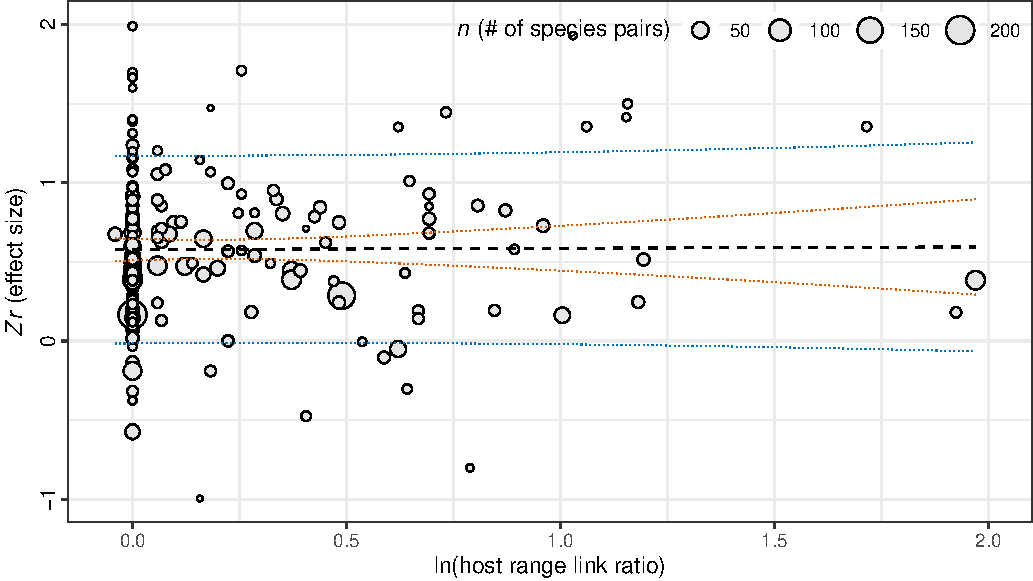
\includegraphics{Supporting_Information_files/figure-latex/unnamed-chunk-25-1.pdf}

\textbf{Supplementary Figure 1:} A bubble plot showing a predicted
regression line for the contentious variable
\texttt{log(host\_range\_link\_ratio)}, indicating 95\% confidence
regions (orange dotted lines) and 95\% prediction regions (blue dotted
lines) with observed effect sizes based on various sample sizes.

\hypertarget{testing-specialization-2-taxonomic-breadth}{%
\paragraph{Testing specialization 2: taxonomic
breadth}\label{testing-specialization-2-taxonomic-breadth}}

\begin{Shaded}
\begin{Highlighting}[]
\CommentTok{# meta-regression}
\NormalTok{mr_host_range_taxonomic_breadth <-}\StringTok{ }\KeywordTok{rma.mv}\NormalTok{(}\DataTypeTok{yi =}\NormalTok{ Zr, }\DataTypeTok{V =}\NormalTok{ VZr, }\DataTypeTok{mods =} \OperatorTok{~}\KeywordTok{log}\NormalTok{(host_range_taxonomic_breadth), }
    \DataTypeTok{random =} \OperatorTok{~}\DecValTok{1} \OperatorTok{|}\StringTok{ }\NormalTok{authors, }\DataTypeTok{data =}\NormalTok{ dat)}
\end{Highlighting}
\end{Shaded}

\textbf{Supplementary Table 6:} Regression coefficients (Estimate), 95\%
confidence intervals (CIs), variance components (V) and variance
explained, \emph{R}\textsuperscript{2}\textsubscript{{[}marginal{]}}
(R2) from the meta-regression with
\texttt{log(host\_range\_taxonomic\_breadth)}.

\begin{Shaded}
\begin{Highlighting}[]
\CommentTok{# getting marginal R2}
\NormalTok{r2_host_range_taxonomic_breadth <-}\StringTok{ }\KeywordTok{R2}\NormalTok{(mr_host_range_taxonomic_breadth)}

\CommentTok{# getting estimates: name does not work for slopes}
\NormalTok{res_host_range_taxonomic_breadth <-}\StringTok{ }\KeywordTok{get_est}\NormalTok{(mr_host_range_taxonomic_breadth, }\DataTypeTok{mod =} \StringTok{"log(host_range_taxonomic_breadth)"}\NormalTok{)}

\CommentTok{# creating a table}
\KeywordTok{tibble}\NormalTok{(}\StringTok{`}\DataTypeTok{Fixed effect}\StringTok{`}\NormalTok{ =}\StringTok{ }\KeywordTok{c}\NormalTok{(}\StringTok{"Intercept"}\NormalTok{, }\StringTok{"log(host_range_taxonomic_breadth)"}\NormalTok{), }\DataTypeTok{Estimate =} \KeywordTok{c}\NormalTok{(res_host_range_taxonomic_breadth}\OperatorTok{$}\NormalTok{estimate), }
    \StringTok{`}\DataTypeTok{Lower CI [0.025]}\StringTok{`}\NormalTok{ =}\StringTok{ }\KeywordTok{c}\NormalTok{(res_host_range_taxonomic_breadth}\OperatorTok{$}\NormalTok{lowerCL), }\StringTok{`}\DataTypeTok{Upper CI  [0.975]}\StringTok{`}\NormalTok{ =}\StringTok{ }\KeywordTok{c}\NormalTok{(res_host_range_taxonomic_breadth}\OperatorTok{$}\NormalTok{upperCL), }
    \StringTok{`}\DataTypeTok{V[authors]}\StringTok{`}\NormalTok{ =}\StringTok{ }\KeywordTok{c}\NormalTok{(mr_host_range_taxonomic_breadth}\OperatorTok{$}\NormalTok{sigma2, }\OtherTok{NA}\NormalTok{), }\DataTypeTok{R2 =} \KeywordTok{c}\NormalTok{(r2_host_range_taxonomic_breadth[}\DecValTok{1}\NormalTok{], }
        \OtherTok{NA}\NormalTok{)) }\OperatorTok\StringTok{ }\KeywordTok{kable}\NormalTok{(}\StringTok{"html"}\NormalTok{, }\DataTypeTok{digits =} \DecValTok{3}\NormalTok{) }\OperatorTok\StringTok{ }\KeywordTok{kable_styling}\NormalTok{(}\StringTok{"striped"}\NormalTok{, }\DataTypeTok{position =} \StringTok{"left"}\NormalTok{)}
\end{Highlighting}
\end{Shaded}

Fixed effect

Estimate

Lower CI {[}0.025{]}

Upper CI {[}0.975{]}

V{[}authors{]}

R2

Intercept

0.590

0.522

0.658

0.088

0

log(host\_range\_taxonomic\_breadth)

0.005

-0.188

0.198

NA

NA

\begin{Shaded}
\begin{Highlighting}[]
\NormalTok{pred_host_range_taxonomic_breadth <-}\KeywordTok{predict.rma}\NormalTok{(mr_host_range_taxonomic_breadth) }

\CommentTok{# plotting}

\NormalTok{fig_host_range_taxonomic_breadth <-}\StringTok{  }\NormalTok{dat }\OperatorTok\StringTok{ }
\StringTok{  }\KeywordTok{filter}\NormalTok{(}\OperatorTok{!}\KeywordTok{is.na}\NormalTok{(host_range_taxonomic_breadth))  }\OperatorTok\StringTok{ }\CommentTok{# getting ride of NA values}
\StringTok{  }\KeywordTok{mutate}\NormalTok{(}\DataTypeTok{ymin =}\NormalTok{ pred_host_range_taxonomic_breadth}\OperatorTok{$}\NormalTok{ci.lb, }
         \DataTypeTok{ymax =}\NormalTok{ pred_host_range_taxonomic_breadth}\OperatorTok{$}\NormalTok{ci.ub,}
         \DataTypeTok{ymin2 =}\NormalTok{ pred_host_range_taxonomic_breadth}\OperatorTok{$}\NormalTok{cr.lb,}
         \DataTypeTok{ymax2 =}\NormalTok{ pred_host_range_taxonomic_breadth}\OperatorTok{$}\NormalTok{cr.ub,}
         \DataTypeTok{pred =}\NormalTok{ pred_host_range_taxonomic_breadth}\OperatorTok{$}\NormalTok{pred) }\OperatorTok\StringTok{ }
\StringTok{  }\KeywordTok{ggplot}\NormalTok{(}\KeywordTok{aes}\NormalTok{(}\DataTypeTok{x =} \KeywordTok{log}\NormalTok{(host_range_taxonomic_breadth), }\DataTypeTok{y =}\NormalTok{ Zr, }\DataTypeTok{size =}\NormalTok{ (}\DecValTok{1}\OperatorTok{/}\NormalTok{VZr) }\OperatorTok{+}\StringTok{ }\DecValTok{3}\NormalTok{, )) }\OperatorTok{+}
\StringTok{  }\KeywordTok{geom_point}\NormalTok{(}\DataTypeTok{shape =} \DecValTok{21}\NormalTok{, }\DataTypeTok{fill =} \StringTok{"grey90"}\NormalTok{) }\OperatorTok{+}
\StringTok{  }\CommentTok{#geom_ribbon(aes(ymin = ymin, ymax = ymax), fill = "#0072B2")  + # not quite sure why this does not work}
\StringTok{  }\KeywordTok{geom_smooth}\NormalTok{(}\KeywordTok{aes}\NormalTok{(}\DataTypeTok{y =}\NormalTok{ ymin2), }\DataTypeTok{method =}  \StringTok{"loess"}\NormalTok{, }\DataTypeTok{se =} \OtherTok{FALSE}\NormalTok{, }\DataTypeTok{lty =}  \StringTok{"dotted"}\NormalTok{, }\DataTypeTok{lwd =} \FloatTok{0.25}\NormalTok{, }\DataTypeTok{colour =} \StringTok{"#0072B2"}\NormalTok{) }\OperatorTok{+}
\StringTok{  }\KeywordTok{geom_smooth}\NormalTok{(}\KeywordTok{aes}\NormalTok{(}\DataTypeTok{y =}\NormalTok{ ymax2), }\DataTypeTok{method =}  \StringTok{"loess"}\NormalTok{, }\DataTypeTok{se =} \OtherTok{FALSE}\NormalTok{, }\DataTypeTok{lty =} \StringTok{"dotted"}\NormalTok{, }\DataTypeTok{lwd =} \FloatTok{0.25}\NormalTok{, }\DataTypeTok{colour =} \StringTok{"#0072B2"}\NormalTok{) }\OperatorTok{+}
\StringTok{  }\KeywordTok{geom_smooth}\NormalTok{(}\KeywordTok{aes}\NormalTok{(}\DataTypeTok{y =}\NormalTok{ ymin), }\DataTypeTok{method =}  \StringTok{"loess"}\NormalTok{, }\DataTypeTok{se =} \OtherTok{FALSE}\NormalTok{,}\DataTypeTok{lty =} \StringTok{"dotted"}\NormalTok{, }\DataTypeTok{lwd =} \FloatTok{0.25}\NormalTok{, }\DataTypeTok{colour =}\StringTok{"#D55E00"}\NormalTok{) }\OperatorTok{+}
\StringTok{  }\KeywordTok{geom_smooth}\NormalTok{(}\KeywordTok{aes}\NormalTok{(}\DataTypeTok{y =}\NormalTok{ ymax), }\DataTypeTok{method =}  \StringTok{"loess"}\NormalTok{, }\DataTypeTok{se =} \OtherTok{FALSE}\NormalTok{, }\DataTypeTok{lty =}\StringTok{"dotted"}\NormalTok{, }\DataTypeTok{lwd =} \FloatTok{0.25}\NormalTok{, }\DataTypeTok{colour =}\StringTok{"#D55E00"}\NormalTok{) }\OperatorTok{+}\StringTok{ }
\StringTok{  }\KeywordTok{geom_smooth}\NormalTok{(}\KeywordTok{aes}\NormalTok{(}\DataTypeTok{y =}\NormalTok{ pred), }\DataTypeTok{method =}  \StringTok{"loess"}\NormalTok{, }\DataTypeTok{se =} \OtherTok{FALSE}\NormalTok{, }\DataTypeTok{lty =}\StringTok{"dashed"}\NormalTok{, }\DataTypeTok{lwd =} \FloatTok{0.5}\NormalTok{, }\DataTypeTok{colour =}\StringTok{"black"}\NormalTok{) }\OperatorTok{+}\StringTok{  }
\StringTok{  }\KeywordTok{ylim}\NormalTok{(}\OperatorTok{-}\DecValTok{1}\NormalTok{, }\DecValTok{2}\NormalTok{) }\OperatorTok{+}\StringTok{ }\KeywordTok{xlim}\NormalTok{(}\DecValTok{0}\NormalTok{, }\FloatTok{1.5}\NormalTok{) }\OperatorTok{+}
\StringTok{  }\CommentTok{#geom_abline(intercept = mr_host_range_link_ratio$beta[[1]], slope = mr_host_range_link_ratio$beta[[2]], alpha = 0.7, linetype = "dashed", size = 0.5) +}
\StringTok{  }\KeywordTok{labs}\NormalTok{(}\DataTypeTok{x =} \StringTok{"ln(host range taxonomic breadth)"}\NormalTok{, }\DataTypeTok{y =} \KeywordTok{expression}\NormalTok{(}\KeywordTok{paste}\NormalTok{(}\KeywordTok{italic}\NormalTok{(Zr), }\StringTok{" (effect size)"}\NormalTok{)), }\DataTypeTok{size =} \KeywordTok{expression}\NormalTok{(}\KeywordTok{paste}\NormalTok{(}\KeywordTok{italic}\NormalTok{(n), }\StringTok{" (# of species pairs)"}\NormalTok{))) }\OperatorTok{+}
\StringTok{  }\KeywordTok{guides}\NormalTok{(}\DataTypeTok{fill =} \StringTok{"none"}\NormalTok{, }\DataTypeTok{colour =} \StringTok{"none"}\NormalTok{) }\OperatorTok{+}
\StringTok{  }\CommentTok{# themses}
\StringTok{  }\KeywordTok{theme_bw}\NormalTok{() }\OperatorTok{+}
\StringTok{  }\KeywordTok{theme}\NormalTok{(}\DataTypeTok{legend.position=} \KeywordTok{c}\NormalTok{(}\DecValTok{1}\NormalTok{, }\DecValTok{1}\NormalTok{), }\DataTypeTok{legend.justification =} \KeywordTok{c}\NormalTok{(}\DecValTok{1}\NormalTok{, }\DecValTok{1}\NormalTok{)) }\OperatorTok{+}
\StringTok{  }\KeywordTok{theme}\NormalTok{(}\DataTypeTok{legend.direction=}\StringTok{"horizontal"}\NormalTok{) }\OperatorTok{+}
\StringTok{  }\CommentTok{#theme(legend.background = element_rect(fill = "white", colour = "black")) +}
\StringTok{  }\KeywordTok{theme}\NormalTok{(}\DataTypeTok{legend.background =} \KeywordTok{element_blank}\NormalTok{()) }\OperatorTok{+}
\StringTok{  }\KeywordTok{theme}\NormalTok{(}\DataTypeTok{axis.text.y =} \KeywordTok{element_text}\NormalTok{(}\DataTypeTok{size =} \DecValTok{10}\NormalTok{, }\DataTypeTok{colour =}\StringTok{"black"}\NormalTok{, }\DataTypeTok{hjust =} \FloatTok{0.5}\NormalTok{, }\DataTypeTok{angle =} \DecValTok{90}\NormalTok{)) }

\NormalTok{fig_host_range_taxonomic_breadth}
\end{Highlighting}
\end{Shaded}

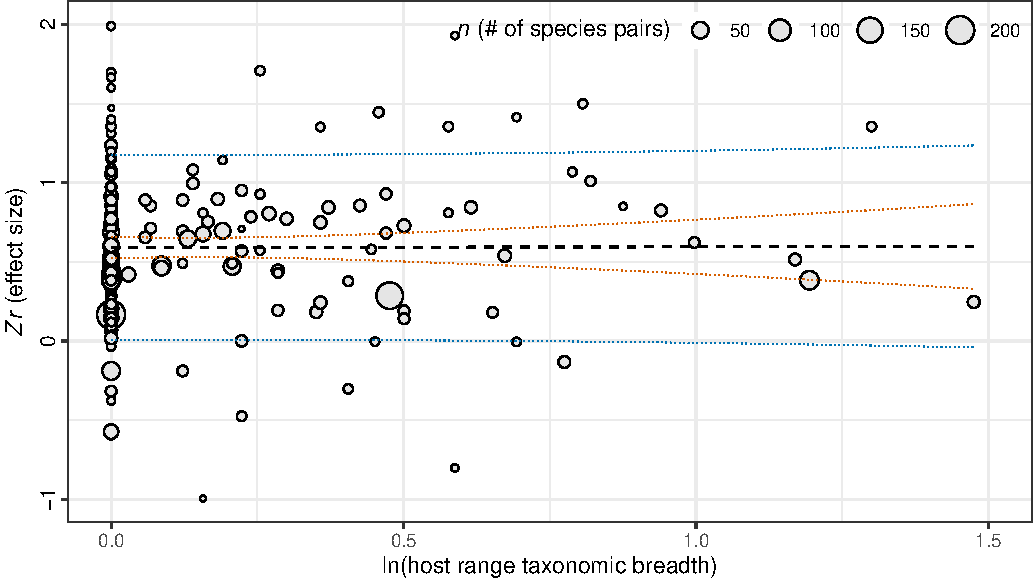
\includegraphics{Supporting_Information_files/figure-latex/unnamed-chunk-28-1.pdf}

\textbf{Supplementary Figure 2:} A bubble plot showing a predicted
regression line for the contentious variable
\texttt{log(log(host\_range\_taxonomic\_breadth)}, indicating 95\%
confidence regions (orange dotted lines) and 95\% prediction regions
(blue dotted lines) with observed effect sizes based on various sample
sizes.

\hypertarget{the-place-of-symbiosis-ednosymbiosis-vs.-ectosymbiosis}{%
\paragraph{The place of symbiosis: ednosymbiosis
vs.~ectosymbiosis}\label{the-place-of-symbiosis-ednosymbiosis-vs.-ectosymbiosis}}

\begin{Shaded}
\begin{Highlighting}[]
\CommentTok{# reordering}
\NormalTok{dat}\OperatorTok{$}\NormalTok{endo_or_ecto <-}\StringTok{ }\KeywordTok{factor}\NormalTok{(dat}\OperatorTok{$}\NormalTok{endo_or_ecto, }\DataTypeTok{levels =} \KeywordTok{c}\NormalTok{(}\StringTok{"Endo/Ecto"}\NormalTok{, }\StringTok{"Endo"}\NormalTok{, }\StringTok{"Ecto"}\NormalTok{))}

\CommentTok{# meta-regression: mutiple intercepts}
\NormalTok{mr_endo_or_ecto1 <-}\StringTok{ }\KeywordTok{rma.mv}\NormalTok{(}\DataTypeTok{yi =}\NormalTok{ Zr, }\DataTypeTok{V =}\NormalTok{ VZr, }\DataTypeTok{mods =} \OperatorTok{~}\NormalTok{endo_or_ecto }\OperatorTok{-}\StringTok{ }\DecValTok{1}\NormalTok{, }\DataTypeTok{test =} \StringTok{"t"}\NormalTok{, }
    \DataTypeTok{random =} \OperatorTok{~}\DecValTok{1} \OperatorTok{|}\StringTok{ }\NormalTok{authors, }\DataTypeTok{data =}\NormalTok{ dat)}

\CommentTok{# meta-regression: contrast 1}
\NormalTok{mr_endo_or_ecto2 <-}\StringTok{ }\KeywordTok{rma.mv}\NormalTok{(}\DataTypeTok{yi =}\NormalTok{ Zr, }\DataTypeTok{V =}\NormalTok{ VZr, }\DataTypeTok{mods =} \OperatorTok{~}\NormalTok{endo_or_ecto, }\DataTypeTok{test =} \StringTok{"t"}\NormalTok{, }\DataTypeTok{random =} \OperatorTok{~}\DecValTok{1} \OperatorTok{|}\StringTok{ }
\StringTok{    }\NormalTok{authors, }\DataTypeTok{data =}\NormalTok{ dat)}

\CommentTok{# meta-regression: contrast 2}
\NormalTok{mr_endo_or_ecto3 <-}\StringTok{ }\KeywordTok{rma.mv}\NormalTok{(}\DataTypeTok{yi =}\NormalTok{ Zr, }\DataTypeTok{V =}\NormalTok{ VZr, }\DataTypeTok{mods =} \OperatorTok{~}\KeywordTok{relevel}\NormalTok{(endo_or_ecto, }\DataTypeTok{ref =} \StringTok{"Endo"}\NormalTok{), }
    \DataTypeTok{test =} \StringTok{"t"}\NormalTok{, }\DataTypeTok{random =} \OperatorTok{~}\DecValTok{1} \OperatorTok{|}\StringTok{ }\NormalTok{authors, }\DataTypeTok{data =}\NormalTok{ dat)}
\end{Highlighting}
\end{Shaded}

\textbf{Supplementary Table 7:} Regression coefficients (estimate), 95\%
confidence intervals (CIs), variance components (V) and variance
explained, \emph{R}\textsuperscript{2}\textsubscript{{[}marginal{]}}
(R2) from the meta-regression with \texttt{endo\_or\_ecto}.

\begin{Shaded}
\begin{Highlighting}[]
\CommentTok{# getting marginal R2}
\NormalTok{r2_endo_or_ecto1 <-}\StringTok{ }\KeywordTok{R2}\NormalTok{(mr_endo_or_ecto1)}

\CommentTok{# getting estimates}
\NormalTok{res_endo_or_ecto1 <-}\StringTok{ }\KeywordTok{get_est}\NormalTok{(mr_endo_or_ecto1, }\DataTypeTok{mod =} \StringTok{"endo_or_ecto"}\NormalTok{)}
\NormalTok{res_endo_or_ecto2 <-}\StringTok{ }\KeywordTok{get_est}\NormalTok{(mr_endo_or_ecto2, }\DataTypeTok{mod =} \StringTok{"endo_or_ecto"}\NormalTok{)}
\NormalTok{res_endo_or_ecto3 <-}\StringTok{ }\KeywordTok{get_est}\NormalTok{(mr_endo_or_ecto3, }\DataTypeTok{mod =} \StringTok{"endo_or_ecto"}\NormalTok{)}

\CommentTok{# creating a table}
\KeywordTok{tibble}\NormalTok{(}\StringTok{`}\DataTypeTok{Fixed effect}\StringTok{`}\NormalTok{ =}\StringTok{ }\KeywordTok{c}\NormalTok{(}\KeywordTok{as.character}\NormalTok{(res_endo_or_ecto1}\OperatorTok{$}\NormalTok{name), }\KeywordTok{cont_gen}\NormalTok{(res_endo_or_ecto1}\OperatorTok{$}\NormalTok{name)), }
    \DataTypeTok{Estimate =} \KeywordTok{c}\NormalTok{(res_endo_or_ecto1}\OperatorTok{$}\NormalTok{estimate, res_endo_or_ecto2}\OperatorTok{$}\NormalTok{estimate[}\OperatorTok{-}\DecValTok{1}\NormalTok{], res_endo_or_ecto3}\OperatorTok{$}\NormalTok{estimate[}\OperatorTok{-}\NormalTok{(}\DecValTok{1}\OperatorTok{:}\DecValTok{2}\NormalTok{)]), }
    \StringTok{`}\DataTypeTok{Lower CI [0.025]}\StringTok{`}\NormalTok{ =}\StringTok{ }\KeywordTok{c}\NormalTok{(res_endo_or_ecto1}\OperatorTok{$}\NormalTok{lowerCL, res_endo_or_ecto2}\OperatorTok{$}\NormalTok{lowerCL[}\OperatorTok{-}\DecValTok{1}\NormalTok{], }
\NormalTok{        res_endo_or_ecto3}\OperatorTok{$}\NormalTok{lowerCL[}\OperatorTok{-}\NormalTok{(}\DecValTok{1}\OperatorTok{:}\DecValTok{2}\NormalTok{)]), }\StringTok{`}\DataTypeTok{Upper CI  [0.975]}\StringTok{`}\NormalTok{ =}\StringTok{ }\KeywordTok{c}\NormalTok{(res_endo_or_ecto1}\OperatorTok{$}\NormalTok{upperCL, }
\NormalTok{        res_endo_or_ecto2}\OperatorTok{$}\NormalTok{upperCL[}\OperatorTok{-}\DecValTok{1}\NormalTok{], res_endo_or_ecto3}\OperatorTok{$}\NormalTok{upperCL[}\OperatorTok{-}\NormalTok{(}\DecValTok{1}\OperatorTok{:}\DecValTok{2}\NormalTok{)]), }\StringTok{`}\DataTypeTok{V[authors]}\StringTok{`}\NormalTok{ =}\StringTok{ }\KeywordTok{c}\NormalTok{(mr_endo_or_ecto1}\OperatorTok{$}\NormalTok{sigma2, }
        \KeywordTok{rep}\NormalTok{(}\OtherTok{NA}\NormalTok{, }\DecValTok{5}\NormalTok{)), }\DataTypeTok{R2 =} \KeywordTok{c}\NormalTok{(r2_endo_or_ecto1[}\DecValTok{1}\NormalTok{], }\KeywordTok{rep}\NormalTok{(}\OtherTok{NA}\NormalTok{, }\DecValTok{5}\NormalTok{))) }\OperatorTok\StringTok{ }\KeywordTok{kable}\NormalTok{(}\StringTok{"html"}\NormalTok{, }\DataTypeTok{digits =} \DecValTok{3}\NormalTok{) }\OperatorTok\StringTok{ }
\StringTok{    }\KeywordTok{kable_styling}\NormalTok{(}\StringTok{"striped"}\NormalTok{, }\DataTypeTok{position =} \StringTok{"left"}\NormalTok{)}
\end{Highlighting}
\end{Shaded}

Fixed effect

Estimate

Lower CI {[}0.025{]}

Upper CI {[}0.975{]}

V{[}authors{]}

R2

Endo/Ecto

0.510

0.029

0.990

0.09

0.004

Endo

0.564

0.491

0.637

NA

NA

Ecto

0.600

0.489

0.710

NA

NA

Endo/Ecto-Endo

0.054

-0.431

0.540

NA

NA

Endo/Ecto-Ecto

0.090

-0.403

0.583

NA

NA

Endo-Ecto

0.036

-0.097

0.168

NA

NA

\begin{Shaded}
\begin{Highlighting}[]
\CommentTok{# getting images}
\NormalTok{image_endoparasite <-}\StringTok{ }\KeywordTok{readPNG}\NormalTok{(}\KeywordTok{here}\NormalTok{(}\StringTok{"images/endoparasite_transparentbg.png"}\NormalTok{))}
\NormalTok{image_ectoparasite <-}\StringTok{ }\KeywordTok{readPNG}\NormalTok{(}\KeywordTok{here}\NormalTok{(}\StringTok{"images/ectoparasite_transparentbg.png"}\NormalTok{))}

\CommentTok{# adding sample size (k) for each category}
\NormalTok{k_endo_or_ecto <-}\StringTok{ }\NormalTok{dat }\OperatorTok\StringTok{ }\KeywordTok{group_by}\NormalTok{(endo_or_ecto) }\OperatorTok\StringTok{ }\KeywordTok{count}\NormalTok{()}
\CommentTok{# getting estimates and predicitons}
\NormalTok{pred_endo_or_ecto <-}\StringTok{ }\KeywordTok{get_pred}\NormalTok{(mr_endo_or_ecto1, }\DataTypeTok{mod =} \StringTok{"endo_or_ecto"}\NormalTok{) }
\NormalTok{res_endo_or_ecto1 <-}\StringTok{ }\KeywordTok{left_join}\NormalTok{(res_endo_or_ecto1, k_endo_or_ecto, }\DataTypeTok{by =}  \KeywordTok{c}\NormalTok{(}\StringTok{"name"}\NormalTok{ =}\StringTok{ "endo_or_ecto"}\NormalTok{))  }\OperatorTok\StringTok{ }\KeywordTok{left_join}\NormalTok{(pred_endo_or_ecto)}
\CommentTok{#res_symbiosis1 }
\CommentTok{# drawing a funnel plot - fig 2b}
\NormalTok{fig_endo_or_ecto <-}\StringTok{ }\KeywordTok{ggplot}\NormalTok{(}\DataTypeTok{data =}\NormalTok{ res_endo_or_ecto1, }\KeywordTok{aes}\NormalTok{(}\DataTypeTok{x =} \KeywordTok{tanh}\NormalTok{(estimate), }\DataTypeTok{y =}\NormalTok{ name)) }\OperatorTok{+}
\StringTok{  }\KeywordTok{scale_x_continuous}\NormalTok{(}\DataTypeTok{limits=}\KeywordTok{c}\NormalTok{(}\OperatorTok{-}\DecValTok{1}\NormalTok{, }\DecValTok{1}\NormalTok{), }\DataTypeTok{breaks =} \KeywordTok{seq}\NormalTok{(}\OperatorTok{-}\DecValTok{1}\NormalTok{, }\DecValTok{1}\NormalTok{, }\DataTypeTok{by =} \FloatTok{0.2}\NormalTok{) ) }\OperatorTok{+}
\StringTok{  }\KeywordTok{geom_quasirandom}\NormalTok{(}\DataTypeTok{data =}\NormalTok{ dat }\OperatorTok\StringTok{ }\KeywordTok{filter}\NormalTok{(}\OperatorTok{!}\KeywordTok{is.na}\NormalTok{(endo_or_ecto)), }
                   \KeywordTok{aes}\NormalTok{(}\DataTypeTok{x=} \KeywordTok{tanh}\NormalTok{(Zr), }\DataTypeTok{y =}\NormalTok{ endo_or_ecto, }\DataTypeTok{size =}\NormalTok{ ((}\DecValTok{1}\OperatorTok{/}\NormalTok{VZr) }\OperatorTok{+}\StringTok{ }\DecValTok{3}\NormalTok{), }\DataTypeTok{colour =}\NormalTok{ endo_or_ecto), }\DataTypeTok{groupOnX =} \OtherTok{FALSE}\NormalTok{, }\DataTypeTok{alpha=}\FloatTok{0.4}\NormalTok{) }\OperatorTok{+}\StringTok{ }
\StringTok{  }\CommentTok{# 95 %precition interval (PI)}
\StringTok{  }\KeywordTok{geom_errorbarh}\NormalTok{(}\KeywordTok{aes}\NormalTok{(}\DataTypeTok{xmin =} \KeywordTok{tanh}\NormalTok{(lowerPR), }\DataTypeTok{xmax =} \KeywordTok{tanh}\NormalTok{(upperPR)),  }\DataTypeTok{height =} \DecValTok{0}\NormalTok{, }\DataTypeTok{show.legend =}\NormalTok{ F, }\DataTypeTok{size =} \FloatTok{0.5}\NormalTok{, }\DataTypeTok{alpha =} \FloatTok{0.6}\NormalTok{) }\OperatorTok{+}
\StringTok{  }\CommentTok{# 95 %CI}
\StringTok{  }\KeywordTok{geom_errorbarh}\NormalTok{(}\KeywordTok{aes}\NormalTok{(}\DataTypeTok{xmin =} \KeywordTok{tanh}\NormalTok{(lowerCL), }\DataTypeTok{xmax =} \KeywordTok{tanh}\NormalTok{(upperCL)),  }\DataTypeTok{height =} \DecValTok{0}\NormalTok{, }\DataTypeTok{show.legend =}\NormalTok{ F, }\DataTypeTok{size =} \FloatTok{1.2}\NormalTok{) }\OperatorTok{+}
\StringTok{  }\KeywordTok{geom_vline}\NormalTok{(}\DataTypeTok{xintercept =} \DecValTok{0}\NormalTok{, }\DataTypeTok{linetype =} \DecValTok{2}\NormalTok{, }\DataTypeTok{colour =} \StringTok{"black"}\NormalTok{, }\DataTypeTok{alpha =} \FloatTok{0.3}\NormalTok{) }\OperatorTok{+}
\StringTok{  }\CommentTok{# creating dots and different size (bee-swarm and bubbles)}
\StringTok{  }\KeywordTok{geom_point}\NormalTok{(}\KeywordTok{aes}\NormalTok{(}\DataTypeTok{fill =}\NormalTok{ name), }\DataTypeTok{size =} \DecValTok{3}\NormalTok{, }\DataTypeTok{shape =} \DecValTok{21}\NormalTok{) }\OperatorTok{+}\StringTok{ }\CommentTok{#}
\StringTok{  }\CommentTok{# setting colours}
\StringTok{  }\KeywordTok{scale_color_manual}\NormalTok{(}\DataTypeTok{values =} \KeywordTok{c}\NormalTok{(}\StringTok{"Endo/Ecto"}\NormalTok{ =}\StringTok{ "#0072B2"}\NormalTok{,  }\StringTok{"Endo"}\NormalTok{ =}\StringTok{ "#D55E00"}\NormalTok{,  }\StringTok{"Ecto"}\NormalTok{=}\StringTok{ "#CC79A7"}\NormalTok{)) }\OperatorTok{+}
\StringTok{  }\KeywordTok{scale_fill_manual}\NormalTok{(}\DataTypeTok{values =} \KeywordTok{c}\NormalTok{(}\StringTok{"Endo/Ecto"}\NormalTok{ =}\StringTok{ "#0072B2"}\NormalTok{,  }\StringTok{"Endo"}\NormalTok{ =}\StringTok{ "#D55E00"}\NormalTok{,  }\StringTok{"Ecto"}\NormalTok{=}\StringTok{ "#CC79A7"}\NormalTok{)) }\OperatorTok{+}
\StringTok{  }\KeywordTok{scale_y_discrete}\NormalTok{(}\DataTypeTok{labels =} \KeywordTok{c}\NormalTok{(}\StringTok{"Endo/Ecto"}\NormalTok{ =}\StringTok{ "Both"}\NormalTok{,  }\StringTok{"Endo"}\NormalTok{ =}\StringTok{ "Endosymbiosis"}\NormalTok{,  }\StringTok{"Ecto"}\NormalTok{=}\StringTok{ "Ectosymbiosis"}\NormalTok{)) }\OperatorTok{+}
\StringTok{  }\KeywordTok{annotate}\NormalTok{(}\StringTok{'text'}\NormalTok{, }\DataTypeTok{x =} \FloatTok{0.93}\NormalTok{, }\DataTypeTok{y =} \DecValTok{1}\OperatorTok{:}\DecValTok{3} \OperatorTok{+}\StringTok{ }\FloatTok{0.15}\NormalTok{, }\DataTypeTok{label=} \KeywordTok{paste}\NormalTok{(}\StringTok{"italic(k)=="}\NormalTok{, res_endo_or_ecto1}\OperatorTok{$}\NormalTok{n), }\DataTypeTok{parse=}\OtherTok{TRUE}\NormalTok{, }\DataTypeTok{hjust =} \StringTok{"left"}\NormalTok{, }\DataTypeTok{size=}\FloatTok{3.5}\NormalTok{) }\OperatorTok{+}
\StringTok{  }\KeywordTok{labs}\NormalTok{(}\DataTypeTok{x =} \KeywordTok{expression}\NormalTok{(}\KeywordTok{paste}\NormalTok{(}\KeywordTok{italic}\NormalTok{(r), }\StringTok{" (correlation)"}\NormalTok{)), }\DataTypeTok{y =} \StringTok{""}\NormalTok{, }\DataTypeTok{size =} \KeywordTok{expression}\NormalTok{(}\KeywordTok{paste}\NormalTok{(}\KeywordTok{italic}\NormalTok{(n), }\StringTok{" (# of species pairs)"}\NormalTok{)) ) }\OperatorTok{+}
\StringTok{  }\KeywordTok{guides}\NormalTok{(}\DataTypeTok{fill =} \StringTok{"none"}\NormalTok{, }\DataTypeTok{colour =} \StringTok{"none"}\NormalTok{) }\OperatorTok{+}
\StringTok{  }\KeywordTok{theme_bw}\NormalTok{() }\OperatorTok{+}
\StringTok{  }\KeywordTok{theme}\NormalTok{(}\DataTypeTok{legend.position=} \KeywordTok{c}\NormalTok{(}\DecValTok{0}\NormalTok{, }\DecValTok{1}\NormalTok{), }\DataTypeTok{legend.justification =} \KeywordTok{c}\NormalTok{(}\DecValTok{0}\NormalTok{,}\DecValTok{1}\NormalTok{)) }\OperatorTok{+}
\StringTok{  }\KeywordTok{theme}\NormalTok{(}\DataTypeTok{legend.direction =} \StringTok{"horizontal"}\NormalTok{) }\OperatorTok{+}
\StringTok{  }\CommentTok{#theme(legend.background = element_rect(fill = "white", colour = "black")) +}
\StringTok{  }\KeywordTok{theme}\NormalTok{(}\DataTypeTok{legend.background =} \KeywordTok{element_blank}\NormalTok{()) }\OperatorTok{+}
\StringTok{  }\KeywordTok{theme}\NormalTok{(}\DataTypeTok{axis.text.y =} \KeywordTok{element_text}\NormalTok{(}\DataTypeTok{size =} \DecValTok{10}\NormalTok{, }\DataTypeTok{colour =}\StringTok{"black"}\NormalTok{, }\DataTypeTok{hjust =} \FloatTok{0.5}\NormalTok{, }\DataTypeTok{angle =} \DecValTok{90}\NormalTok{)) }\OperatorTok{+}
\StringTok{  }\CommentTok{# adding images}
\StringTok{  }\KeywordTok{annotation_custom}\NormalTok{(}\KeywordTok{rasterGrob}\NormalTok{(image_endoparasite), }\DataTypeTok{xmin =} \DecValTok{-1}\NormalTok{, }\DataTypeTok{xmax =} \FloatTok{-0.8}\NormalTok{, }\DataTypeTok{ymin =} \FloatTok{1.6}\NormalTok{, }\DataTypeTok{ymax =} \FloatTok{2.2}\NormalTok{) }\OperatorTok{+}
\StringTok{  }\KeywordTok{annotation_custom}\NormalTok{(}\KeywordTok{rasterGrob}\NormalTok{(image_ectoparasite), }\DataTypeTok{xmin =} \DecValTok{-1}\NormalTok{, }\DataTypeTok{xmax =} \FloatTok{-0.8}\NormalTok{, }\DataTypeTok{ymin =} \FloatTok{2.6}\NormalTok{, }\DataTypeTok{ymax =} \FloatTok{3.2}\NormalTok{) }\OperatorTok{+}\StringTok{ }
\StringTok{  }\KeywordTok{annotation_custom}\NormalTok{(}\KeywordTok{rasterGrob}\NormalTok{(image_ectoparasite), }\DataTypeTok{xmin =} \FloatTok{-1.1}\NormalTok{, }\DataTypeTok{xmax =} \FloatTok{-0.9}\NormalTok{, }\DataTypeTok{ymin =} \FloatTok{0.6}\NormalTok{, }\DataTypeTok{ymax =} \FloatTok{1.2}\NormalTok{) }\OperatorTok{+}\StringTok{ }
\StringTok{  }\KeywordTok{annotation_custom}\NormalTok{(}\KeywordTok{rasterGrob}\NormalTok{(image_endoparasite), }\DataTypeTok{xmin =} \FloatTok{-0.9}\NormalTok{, }\DataTypeTok{xmax =} \FloatTok{-0.7}\NormalTok{, }\DataTypeTok{ymin =} \FloatTok{0.6}\NormalTok{, }\DataTypeTok{ymax =} \FloatTok{1.2}\NormalTok{)}

\NormalTok{fig_endo_or_ecto}
\end{Highlighting}
\end{Shaded}

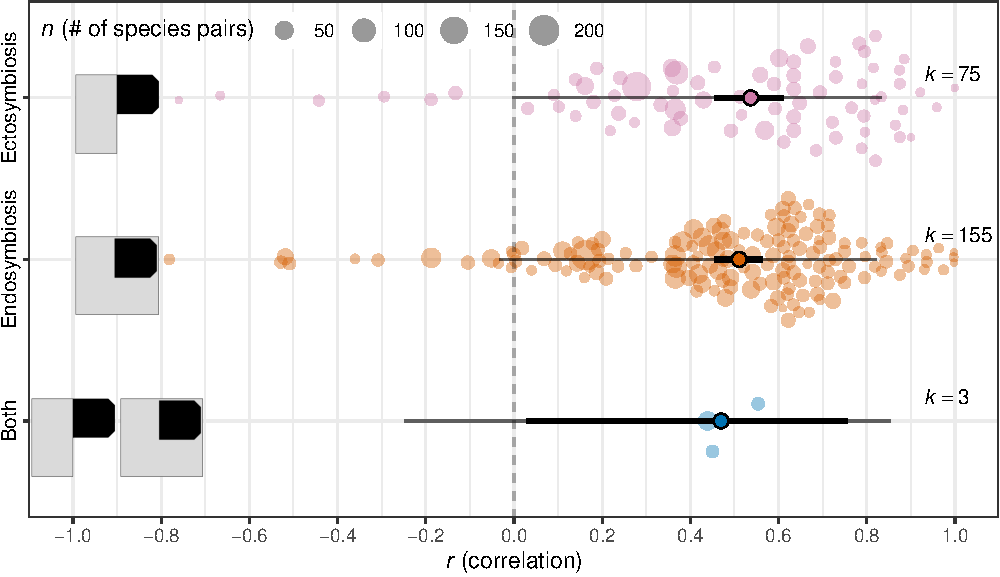
\includegraphics{Supporting_Information_files/figure-latex/unnamed-chunk-31-1.pdf}

\begin{Shaded}
\begin{Highlighting}[]
\CommentTok{# fig 3e}

\NormalTok{e <-}\StringTok{ }\KeywordTok{ggplot}\NormalTok{(}\DataTypeTok{data =}\NormalTok{ res_endo_or_ecto1, }\KeywordTok{aes}\NormalTok{(}\DataTypeTok{x =} \KeywordTok{tanh}\NormalTok{(estimate), }\DataTypeTok{y =}\NormalTok{ name)) }\OperatorTok{+}
\StringTok{  }\KeywordTok{scale_x_continuous}\NormalTok{(}\DataTypeTok{limits=}\KeywordTok{c}\NormalTok{(}\OperatorTok{-}\DecValTok{1}\NormalTok{, }\DecValTok{1}\NormalTok{), }\DataTypeTok{breaks =} \KeywordTok{seq}\NormalTok{(}\OperatorTok{-}\DecValTok{1}\NormalTok{, }\DecValTok{1}\NormalTok{, }\DataTypeTok{by =} \FloatTok{0.2}\NormalTok{) ) }\OperatorTok{+}
\StringTok{  }\KeywordTok{geom_quasirandom}\NormalTok{(}\DataTypeTok{data =}\NormalTok{ dat }\OperatorTok\StringTok{ }\KeywordTok{filter}\NormalTok{(}\OperatorTok{!}\KeywordTok{is.na}\NormalTok{(endo_or_ecto)), }
                   \KeywordTok{aes}\NormalTok{(}\DataTypeTok{x=} \KeywordTok{tanh}\NormalTok{(Zr), }\DataTypeTok{y =}\NormalTok{ endo_or_ecto, }\DataTypeTok{size =}\NormalTok{ ((}\DecValTok{1}\OperatorTok{/}\NormalTok{VZr) }\OperatorTok{+}\StringTok{ }\DecValTok{3}\NormalTok{), }\DataTypeTok{colour =}\NormalTok{ endo_or_ecto), }\DataTypeTok{groupOnX =} \OtherTok{FALSE}\NormalTok{, }\DataTypeTok{alpha=}\FloatTok{0.4}\NormalTok{) }\OperatorTok{+}\StringTok{ }
\StringTok{  }\CommentTok{# 95 %precition interval (PI)}
\StringTok{  }\KeywordTok{geom_errorbarh}\NormalTok{(}\KeywordTok{aes}\NormalTok{(}\DataTypeTok{xmin =} \KeywordTok{tanh}\NormalTok{(lowerPR), }\DataTypeTok{xmax =} \KeywordTok{tanh}\NormalTok{(upperPR)),  }\DataTypeTok{height =} \DecValTok{0}\NormalTok{, }\DataTypeTok{show.legend =}\NormalTok{ F, }\DataTypeTok{size =} \FloatTok{0.5}\NormalTok{, }\DataTypeTok{alpha =} \FloatTok{0.6}\NormalTok{) }\OperatorTok{+}
\StringTok{  }\CommentTok{# 95 %CI}
\StringTok{  }\KeywordTok{geom_errorbarh}\NormalTok{(}\KeywordTok{aes}\NormalTok{(}\DataTypeTok{xmin =} \KeywordTok{tanh}\NormalTok{(lowerCL), }\DataTypeTok{xmax =} \KeywordTok{tanh}\NormalTok{(upperCL)),  }\DataTypeTok{height =} \DecValTok{0}\NormalTok{, }\DataTypeTok{show.legend =}\NormalTok{ F, }\DataTypeTok{size =} \FloatTok{1.2}\NormalTok{) }\OperatorTok{+}
\StringTok{  }\KeywordTok{geom_vline}\NormalTok{(}\DataTypeTok{xintercept =} \DecValTok{0}\NormalTok{, }\DataTypeTok{linetype =} \DecValTok{2}\NormalTok{, }\DataTypeTok{colour =} \StringTok{"black"}\NormalTok{, }\DataTypeTok{alpha =} \FloatTok{0.3}\NormalTok{) }\OperatorTok{+}
\StringTok{  }\CommentTok{# creating dots and different size (bee-swarm and bubbles)}
\StringTok{  }\KeywordTok{geom_point}\NormalTok{(}\KeywordTok{aes}\NormalTok{(}\DataTypeTok{fill =}\NormalTok{ name), }\DataTypeTok{size =} \DecValTok{3}\NormalTok{, }\DataTypeTok{shape =} \DecValTok{21}\NormalTok{) }\OperatorTok{+}\StringTok{ }\CommentTok{#}
\StringTok{  }\CommentTok{# setting colours}
\StringTok{  }\KeywordTok{scale_color_manual}\NormalTok{(}\DataTypeTok{values =} \KeywordTok{c}\NormalTok{(}\StringTok{"Endo/Ecto"}\NormalTok{ =}\StringTok{ "#0072B2"}\NormalTok{,  }\StringTok{"Endo"}\NormalTok{ =}\StringTok{ "#D55E00"}\NormalTok{,  }\StringTok{"Ecto"}\NormalTok{=}\StringTok{ "#CC79A7"}\NormalTok{)) }\OperatorTok{+}
\StringTok{  }\KeywordTok{scale_fill_manual}\NormalTok{(}\DataTypeTok{values =} \KeywordTok{c}\NormalTok{(}\StringTok{"Endo/Ecto"}\NormalTok{ =}\StringTok{ "#0072B2"}\NormalTok{,  }\StringTok{"Endo"}\NormalTok{ =}\StringTok{ "#D55E00"}\NormalTok{,  }\StringTok{"Ecto"}\NormalTok{=}\StringTok{ "#CC79A7"}\NormalTok{)) }\OperatorTok{+}
\StringTok{  }\KeywordTok{scale_y_discrete}\NormalTok{(}\DataTypeTok{labels =} \KeywordTok{c}\NormalTok{(}\StringTok{"Endo/Ecto"}\NormalTok{ =}\StringTok{ "Both"}\NormalTok{,  }\StringTok{"Endo"}\NormalTok{ =}\StringTok{ "Endosymbiosis"}\NormalTok{,  }\StringTok{"Ecto"}\NormalTok{=}\StringTok{ "Ectosymbiosis"}\NormalTok{)) }\OperatorTok{+}
\StringTok{  }\KeywordTok{annotate}\NormalTok{(}\StringTok{'text'}\NormalTok{, }\DataTypeTok{x =} \FloatTok{0.93}\NormalTok{, }\DataTypeTok{y =} \DecValTok{1}\OperatorTok{:}\DecValTok{3} \OperatorTok{+}\StringTok{ }\FloatTok{0.15}\NormalTok{, }\DataTypeTok{label=} \KeywordTok{paste}\NormalTok{(}\StringTok{"italic(k)=="}\NormalTok{, res_endo_or_ecto1}\OperatorTok{$}\NormalTok{n), }\DataTypeTok{parse=}\OtherTok{TRUE}\NormalTok{, }\DataTypeTok{hjust =} \StringTok{"left"}\NormalTok{, }\DataTypeTok{size=}\FloatTok{3.5}\NormalTok{) }\OperatorTok{+}
\StringTok{  }\KeywordTok{labs}\NormalTok{(}\DataTypeTok{x =} \StringTok{""}\NormalTok{, }\DataTypeTok{y =} \StringTok{""}\NormalTok{, }\DataTypeTok{size =} \KeywordTok{expression}\NormalTok{(}\KeywordTok{paste}\NormalTok{(}\KeywordTok{italic}\NormalTok{(n), }\StringTok{" (# of species pairs)"}\NormalTok{)), }\DataTypeTok{tag =} \StringTok{"e"}\NormalTok{ ) }\OperatorTok{+}
\StringTok{  }\KeywordTok{guides}\NormalTok{(}\DataTypeTok{fill =} \StringTok{"none"}\NormalTok{, }\DataTypeTok{colour =} \StringTok{"none"}\NormalTok{) }\OperatorTok{+}
\StringTok{  }\KeywordTok{theme_bw}\NormalTok{() }\OperatorTok{+}
\StringTok{  }\KeywordTok{theme}\NormalTok{(}\DataTypeTok{legend.position=}\StringTok{"none"}\NormalTok{) }\OperatorTok{+}
\StringTok{  }\KeywordTok{theme}\NormalTok{(}\DataTypeTok{axis.text.y =} \KeywordTok{element_text}\NormalTok{(}\DataTypeTok{size =} \DecValTok{10}\NormalTok{, }\DataTypeTok{colour =}\StringTok{"black"}\NormalTok{,}\DataTypeTok{hjust =} \FloatTok{0.5}\NormalTok{, }\DataTypeTok{angle =} \DecValTok{90}\NormalTok{)) }\OperatorTok{+}
\StringTok{  }\CommentTok{# adding images}
\StringTok{  }\KeywordTok{annotation_custom}\NormalTok{(}\KeywordTok{rasterGrob}\NormalTok{(image_endoparasite), }\DataTypeTok{xmin =} \DecValTok{-1}\NormalTok{, }\DataTypeTok{xmax =} \FloatTok{-0.8}\NormalTok{, }\DataTypeTok{ymin =} \FloatTok{1.6}\NormalTok{, }\DataTypeTok{ymax =} \FloatTok{2.2}\NormalTok{) }\OperatorTok{+}
\StringTok{  }\KeywordTok{annotation_custom}\NormalTok{(}\KeywordTok{rasterGrob}\NormalTok{(image_ectoparasite), }\DataTypeTok{xmin =} \DecValTok{-1}\NormalTok{, }\DataTypeTok{xmax =} \FloatTok{-0.8}\NormalTok{, }\DataTypeTok{ymin =} \FloatTok{2.6}\NormalTok{, }\DataTypeTok{ymax =} \FloatTok{3.2}\NormalTok{) }\OperatorTok{+}\StringTok{ }
\StringTok{  }\KeywordTok{annotation_custom}\NormalTok{(}\KeywordTok{rasterGrob}\NormalTok{(image_ectoparasite), }\DataTypeTok{xmin =} \FloatTok{-1.1}\NormalTok{, }\DataTypeTok{xmax =} \FloatTok{-0.9}\NormalTok{, }\DataTypeTok{ymin =} \FloatTok{0.6}\NormalTok{, }\DataTypeTok{ymax =} \FloatTok{1.2}\NormalTok{) }\OperatorTok{+}\StringTok{ }
\StringTok{  }\KeywordTok{annotation_custom}\NormalTok{(}\KeywordTok{rasterGrob}\NormalTok{(image_endoparasite), }\DataTypeTok{xmin =} \FloatTok{-0.9}\NormalTok{, }\DataTypeTok{xmax =} \FloatTok{-0.7}\NormalTok{, }\DataTypeTok{ymin =} \FloatTok{0.6}\NormalTok{, }\DataTypeTok{ymax =} \FloatTok{1.2}\NormalTok{)}
\end{Highlighting}
\end{Shaded}

\textbf{Figure 3e:} A forest plot showing the group-wise means (the
categorical variable \texttt{endo\_or\_ecto}) with their 95\% confidence
intervals (thick lines) and 95\% prediction intervals (thin lines), with
observed effect sizes based on various sample sizes.

\hypertarget{the-effect-of-the-mode-of-transmission}{%
\paragraph{The effect of the mode of
transmission}\label{the-effect-of-the-mode-of-transmission}}

\begin{Shaded}
\begin{Highlighting}[]
\CommentTok{# meta-regression: mutiple intercepts}
\NormalTok{mr_mode_of_transmission_broad1 <-}\StringTok{ }\KeywordTok{rma.mv}\NormalTok{(}\DataTypeTok{yi =}\NormalTok{ Zr, }\DataTypeTok{V =}\NormalTok{ VZr, }\DataTypeTok{mods =} \OperatorTok{~}\NormalTok{mode_of_transmission_broad }\OperatorTok{-}\StringTok{ }
\StringTok{    }\DecValTok{1}\NormalTok{, }\DataTypeTok{test =} \StringTok{"t"}\NormalTok{, }\DataTypeTok{random =} \OperatorTok{~}\DecValTok{1} \OperatorTok{|}\StringTok{ }\NormalTok{authors, }\DataTypeTok{data =}\NormalTok{ dat)}

\CommentTok{# meta-regression: contrast 1}
\NormalTok{mr_mode_of_transmission_broad2 <-}\StringTok{ }\KeywordTok{rma.mv}\NormalTok{(}\DataTypeTok{yi =}\NormalTok{ Zr, }\DataTypeTok{V =}\NormalTok{ VZr, }\DataTypeTok{mods =} \OperatorTok{~}\NormalTok{mode_of_transmission_broad, }
    \DataTypeTok{test =} \StringTok{"t"}\NormalTok{, }\DataTypeTok{random =} \OperatorTok{~}\DecValTok{1} \OperatorTok{|}\StringTok{ }\NormalTok{authors, }\DataTypeTok{data =}\NormalTok{ dat)}

\CommentTok{# meta-regression: contrast 2}
\NormalTok{mr_mode_of_transmission_broad3 <-}\StringTok{ }\KeywordTok{rma.mv}\NormalTok{(}\DataTypeTok{yi =}\NormalTok{ Zr, }\DataTypeTok{V =}\NormalTok{ VZr, }\DataTypeTok{mods =} \OperatorTok{~}\KeywordTok{relevel}\NormalTok{(mode_of_transmission_broad, }
    \DataTypeTok{ref =} \StringTok{"vertical"}\NormalTok{), }\DataTypeTok{test =} \StringTok{"t"}\NormalTok{, }\DataTypeTok{random =} \OperatorTok{~}\DecValTok{1} \OperatorTok{|}\StringTok{ }\NormalTok{authors, }\DataTypeTok{data =}\NormalTok{ dat)}
\end{Highlighting}
\end{Shaded}

\textbf{Supplementary Table 8:} Regression coefficients (estimate), 95\%
confidence intervals (CIs), variance components (V) and variance
explained, \emph{R}\textsuperscript{2}\textsubscript{{[}marginal{]}}
(R2) from the meta-regression with
\texttt{mode\_of\_transmission\_broad}.

\begin{Shaded}
\begin{Highlighting}[]
\CommentTok{# getting marginal R2}
\NormalTok{r2_mode_of_transmission_broad1 <-}\StringTok{ }\KeywordTok{R2}\NormalTok{(mr_mode_of_transmission_broad1)}

\CommentTok{# getting estimates}
\NormalTok{res_mode_of_transmission_broad1 <-}\StringTok{ }\KeywordTok{get_est}\NormalTok{(mr_mode_of_transmission_broad1, }\DataTypeTok{mod =} \StringTok{"mode_of_transmission_broad"}\NormalTok{)}
\NormalTok{res_mode_of_transmission_broad2 <-}\StringTok{ }\KeywordTok{get_est}\NormalTok{(mr_mode_of_transmission_broad2, }\DataTypeTok{mod =} \StringTok{"mode_of_transmission_broad"}\NormalTok{)}
\NormalTok{res_mode_of_transmission_broad3 <-}\StringTok{ }\KeywordTok{get_est}\NormalTok{(mr_mode_of_transmission_broad3, }\DataTypeTok{mod =} \StringTok{"mode_of_transmission_broad"}\NormalTok{)}

\CommentTok{# creating a table}
\KeywordTok{tibble}\NormalTok{(}\StringTok{`}\DataTypeTok{Fixed effect}\StringTok{`}\NormalTok{ =}\StringTok{ }\KeywordTok{c}\NormalTok{(}\KeywordTok{as.character}\NormalTok{(res_mode_of_transmission_broad1}\OperatorTok{$}\NormalTok{name), }\KeywordTok{cont_gen}\NormalTok{(res_mode_of_transmission_broad1}\OperatorTok{$}\NormalTok{name)), }
    \DataTypeTok{Estimate =} \KeywordTok{c}\NormalTok{(res_mode_of_transmission_broad1}\OperatorTok{$}\NormalTok{estimate, res_mode_of_transmission_broad2}\OperatorTok{$}\NormalTok{estimate[}\OperatorTok{-}\DecValTok{1}\NormalTok{], }
\NormalTok{        res_mode_of_transmission_broad3}\OperatorTok{$}\NormalTok{estimate[}\OperatorTok{-}\NormalTok{(}\DecValTok{1}\OperatorTok{:}\DecValTok{2}\NormalTok{)]), }\StringTok{`}\DataTypeTok{Lower CI [0.025]}\StringTok{`}\NormalTok{ =}\StringTok{ }\KeywordTok{c}\NormalTok{(res_mode_of_transmission_broad1}\OperatorTok{$}\NormalTok{lowerCL, }
\NormalTok{        res_mode_of_transmission_broad2}\OperatorTok{$}\NormalTok{lowerCL[}\OperatorTok{-}\DecValTok{1}\NormalTok{], res_mode_of_transmission_broad3}\OperatorTok{$}\NormalTok{lowerCL[}\OperatorTok{-}\NormalTok{(}\DecValTok{1}\OperatorTok{:}\DecValTok{2}\NormalTok{)]), }
    \StringTok{`}\DataTypeTok{Upper CI  [0.975]}\StringTok{`}\NormalTok{ =}\StringTok{ }\KeywordTok{c}\NormalTok{(res_mode_of_transmission_broad1}\OperatorTok{$}\NormalTok{upperCL, res_mode_of_transmission_broad2}\OperatorTok{$}\NormalTok{upperCL[}\OperatorTok{-}\DecValTok{1}\NormalTok{], }
\NormalTok{        res_mode_of_transmission_broad3}\OperatorTok{$}\NormalTok{upperCL[}\OperatorTok{-}\NormalTok{(}\DecValTok{1}\OperatorTok{:}\DecValTok{2}\NormalTok{)]), }\StringTok{`}\DataTypeTok{V[authors]}\StringTok{`}\NormalTok{ =}\StringTok{ }\KeywordTok{c}\NormalTok{(mr_mode_of_transmission_broad1}\OperatorTok{$}\NormalTok{sigma2, }
        \KeywordTok{rep}\NormalTok{(}\OtherTok{NA}\NormalTok{, }\DecValTok{5}\NormalTok{)), }\DataTypeTok{R2 =} \KeywordTok{c}\NormalTok{(r2_mode_of_transmission_broad1[}\DecValTok{1}\NormalTok{], }\KeywordTok{rep}\NormalTok{(}\OtherTok{NA}\NormalTok{, }\DecValTok{5}\NormalTok{))) }\OperatorTok\StringTok{ }\KeywordTok{kable}\NormalTok{(}\StringTok{"html"}\NormalTok{, }
    \DataTypeTok{digits =} \DecValTok{3}\NormalTok{) }\OperatorTok\StringTok{ }\KeywordTok{kable_styling}\NormalTok{(}\StringTok{"striped"}\NormalTok{, }\DataTypeTok{position =} \StringTok{"left"}\NormalTok{)}
\end{Highlighting}
\end{Shaded}

Fixed effect

Estimate

Lower CI {[}0.025{]}

Upper CI {[}0.975{]}

V{[}authors{]}

R2

both

0.620

0.497

0.742

0.068

0.148

horizontal

0.486

0.412

0.559

NA

NA

vertical

0.763

0.642

0.884

NA

NA

both-horizontal

-0.134

-0.277

0.009

NA

NA

both-vertical

0.143

-0.029

0.316

NA

NA

horizontal-vertical

-0.277

-0.419

-0.135

NA

NA

\begin{Shaded}
\begin{Highlighting}[]
\CommentTok{# getting images}
\NormalTok{image_horizontal <-}\StringTok{ }\KeywordTok{readPNG}\NormalTok{(}\KeywordTok{here}\NormalTok{(}\StringTok{"images/horizontal_transparentbg.png"}\NormalTok{))}
\NormalTok{image_vertical <-}\StringTok{ }\KeywordTok{readPNG}\NormalTok{(}\KeywordTok{here}\NormalTok{(}\StringTok{"images/vertical_transparentbg.png"}\NormalTok{))}
\NormalTok{image_both <-}\StringTok{ }\KeywordTok{readPNG}\NormalTok{(}\KeywordTok{here}\NormalTok{(}\StringTok{"images/horizontal_vertical_transparentbg.png"}\NormalTok{))}
\CommentTok{# adding sample size (k) for each category}
\NormalTok{k_mode_of_transmission_broad <-}\StringTok{ }\NormalTok{dat }\OperatorTok\StringTok{ }\KeywordTok{group_by}\NormalTok{(mode_of_transmission_broad) }\OperatorTok\StringTok{ }\KeywordTok{count}\NormalTok{()}
\CommentTok{# getting estimates and predicitons}
\NormalTok{pred_mode_of_transmission_broad <-}\StringTok{ }\KeywordTok{get_pred}\NormalTok{(mr_mode_of_transmission_broad1, }\DataTypeTok{mod =} \StringTok{"mode_of_transmission_broad"}\NormalTok{) }
\NormalTok{res_mode_of_transmission_broad1 <-}\StringTok{ }\KeywordTok{left_join}\NormalTok{(res_mode_of_transmission_broad1, k_mode_of_transmission_broad, }\DataTypeTok{by =}  \KeywordTok{c}\NormalTok{(}\StringTok{"name"}\NormalTok{ =}\StringTok{ "mode_of_transmission_broad"}\NormalTok{))  }\OperatorTok\StringTok{ }\KeywordTok{left_join}\NormalTok{(pred_mode_of_transmission_broad)}
\CommentTok{#res_symbiosis1 }
\CommentTok{# drawing a funnel plot - fig 2b}
\NormalTok{fig_mode_of_transmission_broad <-}\StringTok{ }\KeywordTok{ggplot}\NormalTok{(}\DataTypeTok{data =}\NormalTok{ res_mode_of_transmission_broad1, }\KeywordTok{aes}\NormalTok{(}\DataTypeTok{x =} \KeywordTok{tanh}\NormalTok{(estimate), }\DataTypeTok{y =}\NormalTok{ name)) }\OperatorTok{+}
\StringTok{  }\KeywordTok{scale_x_continuous}\NormalTok{(}\DataTypeTok{limits=}\KeywordTok{c}\NormalTok{(}\OperatorTok{-}\DecValTok{1}\NormalTok{, }\DecValTok{1}\NormalTok{), }\DataTypeTok{breaks =} \KeywordTok{seq}\NormalTok{(}\OperatorTok{-}\DecValTok{1}\NormalTok{, }\DecValTok{1}\NormalTok{, }\DataTypeTok{by =} \FloatTok{0.2}\NormalTok{) ) }\OperatorTok{+}
\StringTok{  }\KeywordTok{geom_quasirandom}\NormalTok{(}\DataTypeTok{data =}\NormalTok{ dat }\OperatorTok\StringTok{ }\KeywordTok{filter}\NormalTok{(}\OperatorTok{!}\KeywordTok{is.na}\NormalTok{(mode_of_transmission_broad)), }
                   \KeywordTok{aes}\NormalTok{(}\DataTypeTok{x=} \KeywordTok{tanh}\NormalTok{(Zr), }\DataTypeTok{y =}\NormalTok{ mode_of_transmission_broad, }\DataTypeTok{size =}\NormalTok{ ((}\DecValTok{1}\OperatorTok{/}\NormalTok{VZr) }\OperatorTok{+}\StringTok{ }\DecValTok{3}\NormalTok{), }\DataTypeTok{colour =}\NormalTok{ mode_of_transmission_broad), }\DataTypeTok{groupOnX =} \OtherTok{FALSE}\NormalTok{, }\DataTypeTok{alpha=}\FloatTok{0.4}\NormalTok{) }\OperatorTok{+}\StringTok{ }
\StringTok{  }\CommentTok{# 95 %precition interval (PI)}
\StringTok{  }\KeywordTok{geom_errorbarh}\NormalTok{(}\KeywordTok{aes}\NormalTok{(}\DataTypeTok{xmin =} \KeywordTok{tanh}\NormalTok{(lowerPR), }\DataTypeTok{xmax =} \KeywordTok{tanh}\NormalTok{(upperPR)),  }\DataTypeTok{height =} \DecValTok{0}\NormalTok{, }\DataTypeTok{show.legend =}\NormalTok{ F, }\DataTypeTok{size =} \FloatTok{0.5}\NormalTok{, }\DataTypeTok{alpha =} \FloatTok{0.6}\NormalTok{) }\OperatorTok{+}
\StringTok{  }\CommentTok{# 95 %CI}
\StringTok{  }\KeywordTok{geom_errorbarh}\NormalTok{(}\KeywordTok{aes}\NormalTok{(}\DataTypeTok{xmin =} \KeywordTok{tanh}\NormalTok{(lowerCL), }\DataTypeTok{xmax =} \KeywordTok{tanh}\NormalTok{(upperCL)),  }\DataTypeTok{height =} \DecValTok{0}\NormalTok{, }\DataTypeTok{show.legend =}\NormalTok{ F, }\DataTypeTok{size =} \FloatTok{1.2}\NormalTok{) }\OperatorTok{+}
\StringTok{  }\KeywordTok{geom_vline}\NormalTok{(}\DataTypeTok{xintercept =} \DecValTok{0}\NormalTok{, }\DataTypeTok{linetype =} \DecValTok{2}\NormalTok{, }\DataTypeTok{colour =} \StringTok{"black"}\NormalTok{, }\DataTypeTok{alpha =} \FloatTok{0.3}\NormalTok{) }\OperatorTok{+}
\StringTok{  }\CommentTok{# creating dots and different size (bee-swarm and bubbles)}
\StringTok{  }\KeywordTok{geom_point}\NormalTok{(}\KeywordTok{aes}\NormalTok{(}\DataTypeTok{fill =}\NormalTok{ name), }\DataTypeTok{size =} \DecValTok{3}\NormalTok{, }\DataTypeTok{shape =} \DecValTok{21}\NormalTok{) }\OperatorTok{+}\StringTok{ }\CommentTok{#}
\StringTok{  }\CommentTok{# setting colours}
\StringTok{  }\KeywordTok{scale_color_manual}\NormalTok{(}\DataTypeTok{values =} \KeywordTok{c}\NormalTok{(}\StringTok{"both"}\NormalTok{ =}\StringTok{ "#0072B2"}\NormalTok{,  }\StringTok{"horizontal"}\NormalTok{ =}\StringTok{ "#D55E00"}\NormalTok{,  }\StringTok{"vertical"}\NormalTok{=}\StringTok{ "#CC79A7"}\NormalTok{)) }\OperatorTok{+}
\StringTok{  }\KeywordTok{scale_fill_manual}\NormalTok{(}\DataTypeTok{values =} \KeywordTok{c}\NormalTok{(}\StringTok{"both"}\NormalTok{ =}\StringTok{ "#0072B2"}\NormalTok{,  }\StringTok{"horizontal"}\NormalTok{ =}\StringTok{ "#D55E00"}\NormalTok{,  }\StringTok{"vertical"}\NormalTok{=}\StringTok{ "#CC79A7"}\NormalTok{)) }\OperatorTok{+}
\StringTok{  }\KeywordTok{scale_y_discrete}\NormalTok{(}\DataTypeTok{labels =} \KeywordTok{c}\NormalTok{(}\StringTok{"both"}\NormalTok{ =}\StringTok{ "Both"}\NormalTok{,  }\StringTok{"horizontal"}\NormalTok{ =}\StringTok{ "Horizontal"}\NormalTok{,  }\StringTok{"vertical"}\NormalTok{=}\StringTok{ "Vertical"}\NormalTok{)) }\OperatorTok{+}
\StringTok{  }\KeywordTok{annotate}\NormalTok{(}\StringTok{'text'}\NormalTok{, }\DataTypeTok{x =} \FloatTok{0.93}\NormalTok{, }\DataTypeTok{y =}\NormalTok{ (}\DecValTok{1}\OperatorTok{:}\DecValTok{3} \OperatorTok{+}\StringTok{ }\FloatTok{0.15}\NormalTok{), }\DataTypeTok{label=} \KeywordTok{paste}\NormalTok{(}\StringTok{"italic(k)=="}\NormalTok{, res_mode_of_transmission_broad1}\OperatorTok{$}\NormalTok{n), }\DataTypeTok{parse=}\OtherTok{TRUE}\NormalTok{, }\DataTypeTok{hjust =} \StringTok{"left"}\NormalTok{, }\DataTypeTok{size=}\FloatTok{3.5}\NormalTok{) }\OperatorTok{+}
\StringTok{  }\KeywordTok{labs}\NormalTok{(}\DataTypeTok{x =} \KeywordTok{expression}\NormalTok{(}\KeywordTok{paste}\NormalTok{(}\KeywordTok{italic}\NormalTok{(r), }\StringTok{" (correlation)"}\NormalTok{)), }\DataTypeTok{y =} \StringTok{""}\NormalTok{, }\DataTypeTok{size =} \KeywordTok{expression}\NormalTok{(}\KeywordTok{paste}\NormalTok{(}\KeywordTok{italic}\NormalTok{(n), }\StringTok{" (# of species pairs)"}\NormalTok{)) ) }\OperatorTok{+}
\StringTok{  }\KeywordTok{guides}\NormalTok{(}\DataTypeTok{fill =} \StringTok{"none"}\NormalTok{, }\DataTypeTok{colour =} \StringTok{"none"}\NormalTok{) }\OperatorTok{+}
\StringTok{  }\KeywordTok{theme_bw}\NormalTok{() }\OperatorTok{+}
\StringTok{  }\KeywordTok{theme}\NormalTok{(}\DataTypeTok{legend.position=} \KeywordTok{c}\NormalTok{(}\DecValTok{0}\NormalTok{, }\DecValTok{1}\NormalTok{), }\DataTypeTok{legend.justification =} \KeywordTok{c}\NormalTok{(}\DecValTok{0}\NormalTok{,}\DecValTok{1}\NormalTok{)) }\OperatorTok{+}
\StringTok{  }\KeywordTok{theme}\NormalTok{(}\DataTypeTok{legend.direction =} \StringTok{"horizontal"}\NormalTok{) }\OperatorTok{+}
\StringTok{  }\CommentTok{#theme(legend.background = element_rect(fill = "white", colour = "black")) +}
\StringTok{  }\KeywordTok{theme}\NormalTok{(}\DataTypeTok{legend.background =} \KeywordTok{element_blank}\NormalTok{()) }\OperatorTok{+}
\StringTok{  }\KeywordTok{theme}\NormalTok{(}\DataTypeTok{axis.text.y =} \KeywordTok{element_text}\NormalTok{(}\DataTypeTok{size =} \DecValTok{10}\NormalTok{, }\DataTypeTok{colour =}\StringTok{"black"}\NormalTok{, }\DataTypeTok{hjust =} \FloatTok{0.5}\NormalTok{, }\DataTypeTok{angle =} \DecValTok{90}\NormalTok{)) }\OperatorTok{+}
\StringTok{  }\CommentTok{# adding images}
\StringTok{  }\KeywordTok{annotation_custom}\NormalTok{(}\KeywordTok{rasterGrob}\NormalTok{(image_horizontal), }\DataTypeTok{xmin =} \DecValTok{-1}\NormalTok{, }\DataTypeTok{xmax =} \FloatTok{-0.7}\NormalTok{, }\DataTypeTok{ymin =} \FloatTok{1.4}\NormalTok{, }\DataTypeTok{ymax =} \FloatTok{2.2}\NormalTok{) }\OperatorTok{+}
\StringTok{  }\KeywordTok{annotation_custom}\NormalTok{(}\KeywordTok{rasterGrob}\NormalTok{(image_vertical), }\DataTypeTok{xmin =} \DecValTok{-1}\NormalTok{, }\DataTypeTok{xmax =} \FloatTok{-0.7}\NormalTok{, }\DataTypeTok{ymin =} \FloatTok{2.4}\NormalTok{, }\DataTypeTok{ymax =} \FloatTok{3.2}\NormalTok{) }\OperatorTok{+}\StringTok{ }
\StringTok{  }\KeywordTok{annotation_custom}\NormalTok{(}\KeywordTok{rasterGrob}\NormalTok{(image_both), }\DataTypeTok{xmin =} \DecValTok{-1}\NormalTok{, }\DataTypeTok{xmax =} \FloatTok{-0.7}\NormalTok{, }\DataTypeTok{ymin =} \FloatTok{0.4}\NormalTok{, }\DataTypeTok{ymax =} \FloatTok{1.2}\NormalTok{) }

\NormalTok{fig_mode_of_transmission_broad}
\end{Highlighting}
\end{Shaded}

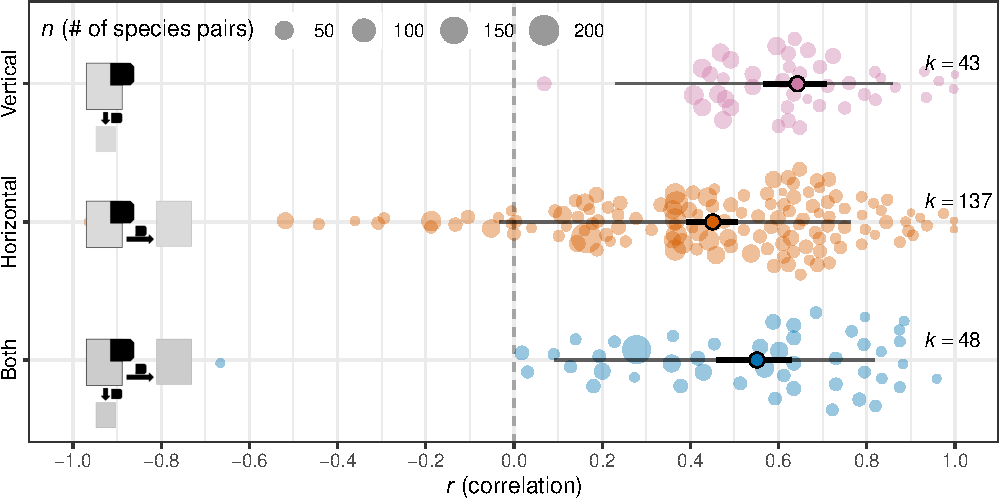
\includegraphics{Supporting_Information_files/figure-latex/unnamed-chunk-34-1.pdf}

\begin{Shaded}
\begin{Highlighting}[]
\CommentTok{# fig 3f}

\NormalTok{f <-}\StringTok{ }\KeywordTok{ggplot}\NormalTok{(}\DataTypeTok{data =}\NormalTok{ res_mode_of_transmission_broad1, }\KeywordTok{aes}\NormalTok{(}\DataTypeTok{x =} \KeywordTok{tanh}\NormalTok{(estimate), }\DataTypeTok{y =}\NormalTok{ name)) }\OperatorTok{+}
\StringTok{  }\KeywordTok{scale_x_continuous}\NormalTok{(}\DataTypeTok{limits=}\KeywordTok{c}\NormalTok{(}\OperatorTok{-}\DecValTok{1}\NormalTok{, }\DecValTok{1}\NormalTok{), }\DataTypeTok{breaks =} \KeywordTok{seq}\NormalTok{(}\OperatorTok{-}\DecValTok{1}\NormalTok{, }\DecValTok{1}\NormalTok{, }\DataTypeTok{by =} \FloatTok{0.2}\NormalTok{) ) }\OperatorTok{+}
\StringTok{  }\KeywordTok{geom_quasirandom}\NormalTok{(}\DataTypeTok{data =}\NormalTok{ dat }\OperatorTok\StringTok{ }\KeywordTok{filter}\NormalTok{(}\OperatorTok{!}\KeywordTok{is.na}\NormalTok{(mode_of_transmission_broad)), }
                   \KeywordTok{aes}\NormalTok{(}\DataTypeTok{x=} \KeywordTok{tanh}\NormalTok{(Zr), }\DataTypeTok{y =}\NormalTok{ mode_of_transmission_broad, }\DataTypeTok{size =}\NormalTok{ ((}\DecValTok{1}\OperatorTok{/}\NormalTok{VZr) }\OperatorTok{+}\StringTok{ }\DecValTok{3}\NormalTok{), }\DataTypeTok{colour =}\NormalTok{ mode_of_transmission_broad), }\DataTypeTok{groupOnX =} \OtherTok{FALSE}\NormalTok{, }\DataTypeTok{alpha=}\FloatTok{0.4}\NormalTok{) }\OperatorTok{+}\StringTok{ }
\StringTok{  }\CommentTok{# 95 %precition interval (PI)}
\StringTok{  }\KeywordTok{geom_errorbarh}\NormalTok{(}\KeywordTok{aes}\NormalTok{(}\DataTypeTok{xmin =} \KeywordTok{tanh}\NormalTok{(lowerPR), }\DataTypeTok{xmax =} \KeywordTok{tanh}\NormalTok{(upperPR)),  }\DataTypeTok{height =} \DecValTok{0}\NormalTok{, }\DataTypeTok{show.legend =}\NormalTok{ F, }\DataTypeTok{size =} \FloatTok{0.5}\NormalTok{, }\DataTypeTok{alpha =} \FloatTok{0.6}\NormalTok{) }\OperatorTok{+}
\StringTok{  }\CommentTok{# 95 %CI}
\StringTok{  }\KeywordTok{geom_errorbarh}\NormalTok{(}\KeywordTok{aes}\NormalTok{(}\DataTypeTok{xmin =} \KeywordTok{tanh}\NormalTok{(lowerCL), }\DataTypeTok{xmax =} \KeywordTok{tanh}\NormalTok{(upperCL)),  }\DataTypeTok{height =} \DecValTok{0}\NormalTok{, }\DataTypeTok{show.legend =}\NormalTok{ F, }\DataTypeTok{size =} \FloatTok{1.2}\NormalTok{) }\OperatorTok{+}
\StringTok{  }\KeywordTok{geom_vline}\NormalTok{(}\DataTypeTok{xintercept =} \DecValTok{0}\NormalTok{, }\DataTypeTok{linetype =} \DecValTok{2}\NormalTok{, }\DataTypeTok{colour =} \StringTok{"black"}\NormalTok{, }\DataTypeTok{alpha =} \FloatTok{0.3}\NormalTok{) }\OperatorTok{+}
\StringTok{  }\CommentTok{# creating dots and different size (bee-swarm and bubbles)}
\StringTok{  }\KeywordTok{geom_point}\NormalTok{(}\KeywordTok{aes}\NormalTok{(}\DataTypeTok{fill =}\NormalTok{ name), }\DataTypeTok{size =} \DecValTok{3}\NormalTok{, }\DataTypeTok{shape =} \DecValTok{21}\NormalTok{) }\OperatorTok{+}\StringTok{ }\CommentTok{#}
\StringTok{  }\CommentTok{# setting colours}
\StringTok{  }\KeywordTok{scale_color_manual}\NormalTok{(}\DataTypeTok{values =} \KeywordTok{c}\NormalTok{(}\StringTok{"both"}\NormalTok{ =}\StringTok{ "#0072B2"}\NormalTok{,  }\StringTok{"horizontal"}\NormalTok{ =}\StringTok{ "#D55E00"}\NormalTok{,  }\StringTok{"vertical"}\NormalTok{=}\StringTok{ "#CC79A7"}\NormalTok{)) }\OperatorTok{+}
\StringTok{  }\KeywordTok{scale_fill_manual}\NormalTok{(}\DataTypeTok{values =} \KeywordTok{c}\NormalTok{(}\StringTok{"both"}\NormalTok{ =}\StringTok{ "#0072B2"}\NormalTok{,  }\StringTok{"horizontal"}\NormalTok{ =}\StringTok{ "#D55E00"}\NormalTok{,  }\StringTok{"vertical"}\NormalTok{=}\StringTok{ "#CC79A7"}\NormalTok{)) }\OperatorTok{+}
\StringTok{  }\KeywordTok{scale_y_discrete}\NormalTok{(}\DataTypeTok{labels =} \KeywordTok{c}\NormalTok{(}\StringTok{"both"}\NormalTok{ =}\StringTok{ "Both"}\NormalTok{,  }\StringTok{"horizontal"}\NormalTok{ =}\StringTok{ "Horizontal"}\NormalTok{,  }\StringTok{"vertical"}\NormalTok{=}\StringTok{ "Vertical"}\NormalTok{)) }\OperatorTok{+}
\StringTok{  }\KeywordTok{annotate}\NormalTok{(}\StringTok{'text'}\NormalTok{, }\DataTypeTok{x =} \FloatTok{0.93}\NormalTok{, }\DataTypeTok{y =}\NormalTok{ (}\DecValTok{1}\OperatorTok{:}\DecValTok{3} \OperatorTok{+}\StringTok{ }\FloatTok{0.15}\NormalTok{), }\DataTypeTok{label=} \KeywordTok{paste}\NormalTok{(}\StringTok{"italic(k)=="}\NormalTok{, res_mode_of_transmission_broad1}\OperatorTok{$}\NormalTok{n), }\DataTypeTok{parse=}\OtherTok{TRUE}\NormalTok{, }\DataTypeTok{hjust =} \StringTok{"left"}\NormalTok{, }\DataTypeTok{size=}\FloatTok{3.5}\NormalTok{) }\OperatorTok{+}
\StringTok{  }\KeywordTok{labs}\NormalTok{(}\DataTypeTok{x =} \StringTok{""}\NormalTok{, }\DataTypeTok{y =} \StringTok{""}\NormalTok{, }\DataTypeTok{size =} \KeywordTok{expression}\NormalTok{(}\KeywordTok{paste}\NormalTok{(}\KeywordTok{italic}\NormalTok{(n), }\StringTok{" (# of species pairs)"}\NormalTok{)), }\DataTypeTok{tag =} \StringTok{"f"}\NormalTok{ ) }\OperatorTok{+}
\StringTok{  }\KeywordTok{guides}\NormalTok{(}\DataTypeTok{fill =} \StringTok{"none"}\NormalTok{, }\DataTypeTok{colour =} \StringTok{"none"}\NormalTok{) }\OperatorTok{+}
\StringTok{  }\KeywordTok{theme_bw}\NormalTok{() }\OperatorTok{+}
\StringTok{  }\KeywordTok{theme}\NormalTok{(}\DataTypeTok{legend.position=}\StringTok{"none"}\NormalTok{) }\OperatorTok{+}
\StringTok{  }\KeywordTok{theme}\NormalTok{(}\DataTypeTok{axis.text.y =} \KeywordTok{element_text}\NormalTok{(}\DataTypeTok{size =} \DecValTok{10}\NormalTok{, }\DataTypeTok{colour =}\StringTok{"black"}\NormalTok{,}\DataTypeTok{hjust =} \FloatTok{0.5}\NormalTok{, }\DataTypeTok{angle =} \DecValTok{90}\NormalTok{)) }\OperatorTok{+}
\StringTok{  }\CommentTok{# adding images}
\StringTok{  }\KeywordTok{annotation_custom}\NormalTok{(}\KeywordTok{rasterGrob}\NormalTok{(image_horizontal), }\DataTypeTok{xmin =} \DecValTok{-1}\NormalTok{, }\DataTypeTok{xmax =} \FloatTok{-0.7}\NormalTok{, }\DataTypeTok{ymin =} \FloatTok{1.4}\NormalTok{, }\DataTypeTok{ymax =} \FloatTok{2.2}\NormalTok{) }\OperatorTok{+}
\StringTok{  }\KeywordTok{annotation_custom}\NormalTok{(}\KeywordTok{rasterGrob}\NormalTok{(image_vertical), }\DataTypeTok{xmin =} \DecValTok{-1}\NormalTok{, }\DataTypeTok{xmax =} \FloatTok{-0.7}\NormalTok{, }\DataTypeTok{ymin =} \FloatTok{2.4}\NormalTok{, }\DataTypeTok{ymax =} \FloatTok{3.2}\NormalTok{) }\OperatorTok{+}\StringTok{ }
\StringTok{  }\KeywordTok{annotation_custom}\NormalTok{(}\KeywordTok{rasterGrob}\NormalTok{(image_both), }\DataTypeTok{xmin =} \DecValTok{-1}\NormalTok{, }\DataTypeTok{xmax =} \FloatTok{-0.7}\NormalTok{, }\DataTypeTok{ymin =} \FloatTok{0.4}\NormalTok{, }\DataTypeTok{ymax =} \FloatTok{1.2}\NormalTok{) }
\end{Highlighting}
\end{Shaded}

\textbf{Figure 2f:} A forest plot showing the group-wise means (the
categorical variable \texttt{mode\_of\_transmission\_broad}), indicating
95\% confidence intervals (thick lines) and 95\% prediction intervals
(thin lines), with observed effect sizes based on various sample sizes.

\hypertarget{the-combined-effect-of-symbiosis-and-mode-of-transmission}{%
\paragraph{The combined effect of symbiosis and mode of
transmission}\label{the-combined-effect-of-symbiosis-and-mode-of-transmission}}

\begin{Shaded}
\begin{Highlighting}[]
\CommentTok{# reordering}
\NormalTok{dat}\OperatorTok{$}\NormalTok{symbiosis_transmission <-}\StringTok{ }\KeywordTok{factor}\NormalTok{(dat}\OperatorTok{$}\NormalTok{symbiosis_transmission, }\DataTypeTok{levels =} \KeywordTok{c}\NormalTok{(}\StringTok{"Mutualistboth"}\NormalTok{, }
    \StringTok{"Mutualisthorizontal"}\NormalTok{, }\StringTok{"Mutualistvertical"}\NormalTok{, }\StringTok{"Parasiteboth"}\NormalTok{, }\StringTok{"Parasitehorizontal"}\NormalTok{), }
    \DataTypeTok{labels =} \KeywordTok{c}\NormalTok{(}\StringTok{"MutualistBoth"}\NormalTok{, }\StringTok{"MutualistHorizontal"}\NormalTok{, }\StringTok{"MutualistVertical"}\NormalTok{, }\StringTok{"ParasiteBoth"}\NormalTok{, }
        \StringTok{"ParasiteHorizontal"}\NormalTok{))}

\CommentTok{# meta-regression: mutiple intercepts}
\NormalTok{mr_symbiosis_transmission1 <-}\StringTok{ }\KeywordTok{rma.mv}\NormalTok{(}\DataTypeTok{yi =}\NormalTok{ Zr, }\DataTypeTok{V =}\NormalTok{ VZr, }\DataTypeTok{mods =} \OperatorTok{~}\NormalTok{symbiosis_transmission }\OperatorTok{-}\StringTok{ }
\StringTok{    }\DecValTok{1}\NormalTok{, }\DataTypeTok{test =} \StringTok{"t"}\NormalTok{, }\DataTypeTok{random =} \OperatorTok{~}\DecValTok{1} \OperatorTok{|}\StringTok{ }\NormalTok{authors, }\DataTypeTok{data =}\NormalTok{ dat)}

\CommentTok{# # meta-regression: contrasts x 10 getting the level names out}
\NormalTok{level_names <-}\StringTok{ }\KeywordTok{levels}\NormalTok{(dat}\OperatorTok{$}\NormalTok{symbiosis_transmission)}

\CommentTok{# helper function to run metafor meta-regression}
\NormalTok{run_rma <-}\StringTok{ }\ControlFlowTok{function}\NormalTok{(name) \{}
    \KeywordTok{rma.mv}\NormalTok{(}\DataTypeTok{yi =}\NormalTok{ Zr, }\DataTypeTok{V =}\NormalTok{ VZr, }\DataTypeTok{mods =} \OperatorTok{~}\KeywordTok{relevel}\NormalTok{(symbiosis_transmission, }\DataTypeTok{ref =}\NormalTok{ name), }
        \DataTypeTok{test =} \StringTok{"t"}\NormalTok{, }\DataTypeTok{random =} \OperatorTok{~}\DecValTok{1} \OperatorTok{|}\StringTok{ }\NormalTok{authors, }\DataTypeTok{data =}\NormalTok{ dat)}
\NormalTok{\}}

\CommentTok{# results of meta-regression including all contrast results; taking the last}
\CommentTok{# level out ([-length(level_names)])}
\NormalTok{mr_symbiosis_transmission <-}\StringTok{ }\KeywordTok{map}\NormalTok{(level_names[}\OperatorTok{-}\KeywordTok{length}\NormalTok{(level_names)], run_rma)}
\end{Highlighting}
\end{Shaded}

\textbf{Supplementary Table 9:} Regression coefficients (estimate), 95\%
confidence intervals (CIs), variance components (V) and variance
explained, \emph{R}\textsuperscript{2}\textsubscript{{[}marginal{]}}
(R2) from the meta-regression with \texttt{symbiosis\_transmission}.

\begin{Shaded}
\begin{Highlighting}[]
\CommentTok{# getting marginal R2}
\NormalTok{r2_symbiosis_transmission1 <-}\StringTok{ }\KeywordTok{R2}\NormalTok{(mr_symbiosis_transmission1)}

\CommentTok{# getting estimates}
\NormalTok{res_symbiosis_transmission1 <-}\StringTok{ }\KeywordTok{get_est}\NormalTok{(mr_symbiosis_transmission1, }\DataTypeTok{mod =} \StringTok{"symbiosis_transmission"}\NormalTok{)}
\NormalTok{res_symbiosis_transmission <-}\StringTok{ }\KeywordTok{map}\NormalTok{(mr_symbiosis_transmission, }\OperatorTok{~}\KeywordTok{get_est}\NormalTok{(.x, }\DataTypeTok{mod =} \StringTok{"symbiosis_transmission"}\NormalTok{))}

\CommentTok{# a list of the numbers to take out unnecessary contrasts}
\NormalTok{contra_list <-}\StringTok{ }\KeywordTok{Map}\NormalTok{(seq, }\DataTypeTok{from =} \DecValTok{1}\NormalTok{, }\DataTypeTok{to =} \DecValTok{1}\OperatorTok{:}\DecValTok{4}\NormalTok{)}

\CommentTok{# you need to flatten twice: first to make it a list and make it a vector}
\NormalTok{estimates <-}\StringTok{ }\KeywordTok{map2}\NormalTok{(res_symbiosis_transmission, contra_list, }\OperatorTok{~}\NormalTok{.x[}\OperatorTok{-}\NormalTok{(.y), }\StringTok{"estimate"}\NormalTok{]) }\OperatorTok\StringTok{ }
\StringTok{    }\KeywordTok{flatten}\NormalTok{() }\OperatorTok\StringTok{ }\KeywordTok{flatten_dbl}\NormalTok{()}
\NormalTok{lowerCLs <-}\StringTok{ }\KeywordTok{map2}\NormalTok{(res_symbiosis_transmission, contra_list, }\OperatorTok{~}\NormalTok{.x[}\OperatorTok{-}\NormalTok{(.y), }\StringTok{"lowerCL"}\NormalTok{]) }\OperatorTok\StringTok{ }
\StringTok{    }\KeywordTok{flatten}\NormalTok{() }\OperatorTok\StringTok{ }\KeywordTok{flatten_dbl}\NormalTok{()}
\NormalTok{upperCLs <-}\StringTok{ }\KeywordTok{map2}\NormalTok{(res_symbiosis_transmission, contra_list, }\OperatorTok{~}\NormalTok{.x[}\OperatorTok{-}\NormalTok{(.y), }\StringTok{"upperCL"}\NormalTok{]) }\OperatorTok\StringTok{ }
\StringTok{    }\KeywordTok{flatten}\NormalTok{() }\OperatorTok\StringTok{ }\KeywordTok{flatten_dbl}\NormalTok{()}

\CommentTok{# creating a table}
\KeywordTok{tibble}\NormalTok{(}\StringTok{`}\DataTypeTok{Fixed effect}\StringTok{`}\NormalTok{ =}\StringTok{ }\KeywordTok{c}\NormalTok{(}\KeywordTok{as.character}\NormalTok{(res_symbiosis_transmission1}\OperatorTok{$}\NormalTok{name), }\KeywordTok{cont_gen}\NormalTok{(res_symbiosis_transmission1}\OperatorTok{$}\NormalTok{name)), }
    \DataTypeTok{Estimate =} \KeywordTok{c}\NormalTok{(res_symbiosis_transmission1}\OperatorTok{$}\NormalTok{estimate, estimates), }\StringTok{`}\DataTypeTok{Lower CI [0.025]}\StringTok{`}\NormalTok{ =}\StringTok{ }\KeywordTok{c}\NormalTok{(res_symbiosis_transmission1}\OperatorTok{$}\NormalTok{lowerCL, }
\NormalTok{        lowerCLs), }\StringTok{`}\DataTypeTok{Upper CI  [0.975]}\StringTok{`}\NormalTok{ =}\StringTok{ }\KeywordTok{c}\NormalTok{(res_symbiosis_transmission1}\OperatorTok{$}\NormalTok{upperCL, upperCLs), }
    \StringTok{`}\DataTypeTok{V[authors]}\StringTok{`}\NormalTok{ =}\StringTok{ }\KeywordTok{c}\NormalTok{(mr_symbiosis_transmission1}\OperatorTok{$}\NormalTok{sigma2, }\KeywordTok{rep}\NormalTok{(}\OtherTok{NA}\NormalTok{, (}\DecValTok{5} \OperatorTok{+}\StringTok{ }\KeywordTok{choose}\NormalTok{(}\DecValTok{5}\NormalTok{, }\DecValTok{2}\NormalTok{)) }\OperatorTok{-}\StringTok{ }
\StringTok{        }\DecValTok{1}\NormalTok{)), }\DataTypeTok{R2 =} \KeywordTok{c}\NormalTok{(r2_symbiosis_transmission1[}\DecValTok{1}\NormalTok{], }\KeywordTok{rep}\NormalTok{(}\OtherTok{NA}\NormalTok{, (}\DecValTok{5} \OperatorTok{+}\StringTok{ }\KeywordTok{choose}\NormalTok{(}\DecValTok{5}\NormalTok{, }\DecValTok{2}\NormalTok{)) }\OperatorTok{-}\StringTok{ }\DecValTok{1}\NormalTok{))) }\OperatorTok\StringTok{ }
\StringTok{    }\KeywordTok{kable}\NormalTok{(}\StringTok{"html"}\NormalTok{, }\DataTypeTok{digits =} \DecValTok{3}\NormalTok{) }\OperatorTok\StringTok{ }\KeywordTok{kable_styling}\NormalTok{(}\StringTok{"striped"}\NormalTok{, }\DataTypeTok{position =} \StringTok{"left"}\NormalTok{) }\OperatorTok\StringTok{ }
\StringTok{    }\KeywordTok{scroll_box}\NormalTok{(}\DataTypeTok{width =} \StringTok{"100%"}\NormalTok{, }\DataTypeTok{height =} \StringTok{"300px"}\NormalTok{)}
\end{Highlighting}
\end{Shaded}

Fixed effect

Estimate

Lower CI {[}0.025{]}

Upper CI {[}0.975{]}

V{[}authors{]}

R2

MutualistBoth

0.719

0.349

1.089

0.069

0.142

MutualistHorizontal

0.490

0.322

0.659

NA

NA

MutualistVertical

0.757

0.635

0.880

NA

NA

ParasiteBoth

0.608

0.477

0.739

NA

NA

ParasiteHorizontal

0.486

0.405

0.566

NA

NA

MutualistBoth-MutualistHorizontal

-0.229

-0.635

0.178

NA

NA

MutualistBoth-MutualistVertical

0.038

-0.352

0.428

NA

NA

MutualistBoth-ParasiteBoth

-0.111

-0.504

0.281

NA

NA

MutualistBoth-ParasiteHorizontal

-0.234

-0.612

0.145

NA

NA

MutualistHorizontal-MutualistVertical

0.267

0.059

0.475

NA

NA

MutualistHorizontal-ParasiteBoth

0.118

-0.095

0.331

NA

NA

MutualistHorizontal-ParasiteHorizontal

-0.005

-0.187

0.177

NA

NA

MutualistVertical-ParasiteBoth

-0.149

-0.329

0.030

NA

NA

MutualistVertical-ParasiteHorizontal

-0.272

-0.419

-0.125

NA

NA

ParasiteBoth-ParasiteHorizontal

-0.122

-0.276

0.031

NA

NA

\begin{Shaded}
\begin{Highlighting}[]
\CommentTok{# colour list}
\NormalTok{colour_ls <-}\StringTok{ }\KeywordTok{c}\NormalTok{(}\StringTok{"#000000"}\NormalTok{, }\StringTok{"#E69F00"}\NormalTok{, }\StringTok{"#56B4E9"}\NormalTok{, }\StringTok{"#009E73"}\NormalTok{,  }\StringTok{"#F0E422"}\NormalTok{,  }\StringTok{"#0072B2"}\NormalTok{,  }\StringTok{"#D55E00"}\NormalTok{, }\StringTok{"#CC79A7"}\NormalTok{, }\StringTok{"#00008B"}\NormalTok{, }\StringTok{"#8B0A50"}\NormalTok{, }\StringTok{"#54FF9F"}\NormalTok{, }\StringTok{"#999999"}\NormalTok{)}

\CommentTok{# adding sample size (k) for each category}
\NormalTok{k_symbiosis_transmission <-}\StringTok{ }\NormalTok{dat }\OperatorTok\StringTok{ }\KeywordTok{group_by}\NormalTok{(symbiosis_transmission) }\OperatorTok\StringTok{ }\KeywordTok{count}\NormalTok{()}
\CommentTok{# getting estimates and predicitons}
\NormalTok{pred_symbiosis_transmission <-}\StringTok{ }\KeywordTok{get_pred}\NormalTok{(mr_symbiosis_transmission1, }\DataTypeTok{mod =} \StringTok{"symbiosis_transmission"}\NormalTok{) }
\NormalTok{res_symbiosis_transmission1 <-}\StringTok{ }\KeywordTok{left_join}\NormalTok{(res_symbiosis_transmission1, k_symbiosis_transmission, }\DataTypeTok{by =}  \KeywordTok{c}\NormalTok{(}\StringTok{"name"}\NormalTok{ =}\StringTok{ "symbiosis_transmission"}\NormalTok{))  }\OperatorTok\StringTok{ }\KeywordTok{left_join}\NormalTok{(pred_symbiosis_transmission)}
\CommentTok{#res_symbiosis1 }
\CommentTok{# drawing a funnel plot - fig 2b}
\NormalTok{fig_symbiosis_transmission <-}\StringTok{ }\KeywordTok{ggplot}\NormalTok{(}\DataTypeTok{data =}\NormalTok{ res_symbiosis_transmission1, }\KeywordTok{aes}\NormalTok{(}\DataTypeTok{x =} \KeywordTok{tanh}\NormalTok{(estimate), }\DataTypeTok{y =}\NormalTok{ name)) }\OperatorTok{+}
\StringTok{  }\KeywordTok{scale_x_continuous}\NormalTok{(}\DataTypeTok{limits=}\KeywordTok{c}\NormalTok{(}\OperatorTok{-}\DecValTok{1}\NormalTok{, }\DecValTok{1}\NormalTok{), }\DataTypeTok{breaks =} \KeywordTok{seq}\NormalTok{(}\OperatorTok{-}\DecValTok{1}\NormalTok{, }\DecValTok{1}\NormalTok{, }\DataTypeTok{by =} \FloatTok{0.2}\NormalTok{) ) }\OperatorTok{+}
\StringTok{  }\KeywordTok{geom_quasirandom}\NormalTok{(}\DataTypeTok{data =}\NormalTok{ dat }\OperatorTok\StringTok{ }\KeywordTok{filter}\NormalTok{(}\OperatorTok{!}\KeywordTok{is.na}\NormalTok{(symbiosis_transmission)), }
                   \KeywordTok{aes}\NormalTok{(}\DataTypeTok{x=} \KeywordTok{tanh}\NormalTok{(Zr), }\DataTypeTok{y =}\NormalTok{ symbiosis_transmission, }\DataTypeTok{size =}\NormalTok{ ((}\DecValTok{1}\OperatorTok{/}\NormalTok{VZr) }\OperatorTok{+}\StringTok{ }\DecValTok{3}\NormalTok{), }\DataTypeTok{colour =}\NormalTok{ symbiosis_transmission), }\DataTypeTok{groupOnX =} \OtherTok{FALSE}\NormalTok{, }\DataTypeTok{alpha=}\FloatTok{0.4}\NormalTok{) }\OperatorTok{+}\StringTok{ }
\StringTok{  }\CommentTok{# 95 %precition interval (PI)}
\StringTok{  }\KeywordTok{geom_errorbarh}\NormalTok{(}\KeywordTok{aes}\NormalTok{(}\DataTypeTok{xmin =} \KeywordTok{tanh}\NormalTok{(lowerPR), }\DataTypeTok{xmax =} \KeywordTok{tanh}\NormalTok{(upperPR)),  }\DataTypeTok{height =} \DecValTok{0}\NormalTok{, }\DataTypeTok{show.legend =}\NormalTok{ F, }\DataTypeTok{size =} \FloatTok{0.5}\NormalTok{, }\DataTypeTok{alpha =} \FloatTok{0.6}\NormalTok{) }\OperatorTok{+}
\StringTok{  }\CommentTok{# 95 %CI}
\StringTok{  }\KeywordTok{geom_errorbarh}\NormalTok{(}\KeywordTok{aes}\NormalTok{(}\DataTypeTok{xmin =} \KeywordTok{tanh}\NormalTok{(lowerCL), }\DataTypeTok{xmax =} \KeywordTok{tanh}\NormalTok{(upperCL)),  }\DataTypeTok{height =} \DecValTok{0}\NormalTok{, }\DataTypeTok{show.legend =}\NormalTok{ F, }\DataTypeTok{size =} \FloatTok{1.2}\NormalTok{) }\OperatorTok{+}
\StringTok{  }\KeywordTok{geom_vline}\NormalTok{(}\DataTypeTok{xintercept =} \DecValTok{0}\NormalTok{, }\DataTypeTok{linetype =} \DecValTok{2}\NormalTok{, }\DataTypeTok{colour =} \StringTok{"black"}\NormalTok{, }\DataTypeTok{alpha =} \FloatTok{0.3}\NormalTok{) }\OperatorTok{+}
\StringTok{  }\CommentTok{# creating dots and different size (bee-swarm and bubbles)}
\StringTok{  }\KeywordTok{geom_point}\NormalTok{(}\KeywordTok{aes}\NormalTok{(}\DataTypeTok{fill =}\NormalTok{ name), }\DataTypeTok{size =} \DecValTok{3}\NormalTok{, }\DataTypeTok{shape =} \DecValTok{21}\NormalTok{) }\OperatorTok{+}\StringTok{ }\CommentTok{#}
\StringTok{  }\CommentTok{# setting colours}
\StringTok{  }\KeywordTok{scale_color_manual}\NormalTok{(}\DataTypeTok{values =}   \KeywordTok{c}\NormalTok{(}\StringTok{"MutualistBoth"}\NormalTok{=}\StringTok{ }\NormalTok{colour_ls[}\DecValTok{1}\NormalTok{], }\StringTok{"MutualistHorizontal"}\NormalTok{=}\StringTok{ }\NormalTok{colour_ls[}\DecValTok{2}\NormalTok{], }\StringTok{"MutualistVertical"}\NormalTok{ =}\StringTok{ }\NormalTok{colour_ls[}\DecValTok{3}\NormalTok{],}\StringTok{"ParasiteBoth"}\NormalTok{=}\StringTok{ }\NormalTok{colour_ls[}\DecValTok{4}\NormalTok{], }\StringTok{"ParasiteHorizontal"}\NormalTok{ =}\StringTok{ }\NormalTok{colour_ls[}\DecValTok{5}\NormalTok{])) }\OperatorTok{+}
\StringTok{  }\KeywordTok{scale_fill_manual}\NormalTok{(}\DataTypeTok{values =} \KeywordTok{c}\NormalTok{(}\StringTok{"MutualistBoth"}\NormalTok{=}\StringTok{ }\NormalTok{colour_ls[}\DecValTok{1}\NormalTok{], }\StringTok{"MutualistHorizontal"}\NormalTok{=}\StringTok{ }\NormalTok{colour_ls[}\DecValTok{2}\NormalTok{], }\StringTok{"MutualistVertical"}\NormalTok{ =}\StringTok{ }\NormalTok{colour_ls[}\DecValTok{3}\NormalTok{],}\StringTok{"ParasiteBoth"}\NormalTok{=}\StringTok{ }\NormalTok{colour_ls[}\DecValTok{4}\NormalTok{], }\StringTok{"ParasiteHorizontal"}\NormalTok{ =}\StringTok{ }\NormalTok{colour_ls[}\DecValTok{5}\NormalTok{])) }\OperatorTok{+}
\StringTok{  }\KeywordTok{scale_y_discrete}\NormalTok{(}\DataTypeTok{labels =} \KeywordTok{c}\NormalTok{(}\StringTok{"MutualistBoth"}\NormalTok{ =}\StringTok{ "Mutualist-}\CharTok{\textbackslash{}n}\StringTok{Both"}\NormalTok{, }\StringTok{"MutualistHorizontal"}\NormalTok{ =}\StringTok{ "Mutualist-}\CharTok{\textbackslash{}n}\StringTok{Horizontal"}\NormalTok{,}\StringTok{"MutualistVertical"}\NormalTok{ =}\StringTok{ "Mutualist-}\CharTok{\textbackslash{}n}\StringTok{Vertical"}\NormalTok{, }\StringTok{"ParasiteBoth"}\NormalTok{ =}\StringTok{ "Parasite-}\CharTok{\textbackslash{}n}\StringTok{Both"}\NormalTok{, }\StringTok{"ParasiteHorizontal"}\NormalTok{ =}\StringTok{ "Parasite-}\CharTok{\textbackslash{}n}\StringTok{Horizontal"}\NormalTok{)) }\OperatorTok{+}
\StringTok{  }\KeywordTok{annotate}\NormalTok{(}\StringTok{'text'}\NormalTok{, }\DataTypeTok{x =} \FloatTok{0.93}\NormalTok{, }\DataTypeTok{y =} \DecValTok{1}\OperatorTok{:}\DecValTok{5} \OperatorTok{+}\StringTok{ }\FloatTok{0.15}\NormalTok{, }\DataTypeTok{label=} \KeywordTok{paste}\NormalTok{(}\StringTok{"italic(k)=="}\NormalTok{, res_symbiosis_transmission1}\OperatorTok{$}\NormalTok{n), }\DataTypeTok{parse=}\OtherTok{TRUE}\NormalTok{, }\DataTypeTok{hjust =} \StringTok{"left"}\NormalTok{, }\DataTypeTok{size=}\FloatTok{3.5}\NormalTok{) }\OperatorTok{+}
\StringTok{  }\KeywordTok{labs}\NormalTok{(}\DataTypeTok{x =} \KeywordTok{expression}\NormalTok{(}\KeywordTok{paste}\NormalTok{(}\KeywordTok{italic}\NormalTok{(r), }\StringTok{" (correlation)"}\NormalTok{)), }\DataTypeTok{y =} \StringTok{""}\NormalTok{, }\DataTypeTok{size =} \KeywordTok{expression}\NormalTok{(}\KeywordTok{paste}\NormalTok{(}\KeywordTok{italic}\NormalTok{(n), }\StringTok{" (# of species pairs)"}\NormalTok{)) ) }\OperatorTok{+}
\StringTok{  }\KeywordTok{guides}\NormalTok{(}\DataTypeTok{fill =} \StringTok{"none"}\NormalTok{, }\DataTypeTok{colour =} \StringTok{"none"}\NormalTok{) }\OperatorTok{+}
\StringTok{  }\KeywordTok{theme_bw}\NormalTok{() }\OperatorTok{+}
\StringTok{  }\KeywordTok{theme}\NormalTok{(}\DataTypeTok{legend.position=} \KeywordTok{c}\NormalTok{(}\DecValTok{0}\NormalTok{, }\DecValTok{1}\NormalTok{), }\DataTypeTok{legend.justification =} \KeywordTok{c}\NormalTok{(}\DecValTok{0}\NormalTok{,}\DecValTok{1}\NormalTok{)) }\OperatorTok{+}
\StringTok{  }\KeywordTok{theme}\NormalTok{(}\DataTypeTok{legend.direction=}\StringTok{"horizontal"}\NormalTok{) }\OperatorTok{+}
\StringTok{  }\CommentTok{#theme(legend.background = element_rect(fill = "white", colour = "black")) +}
\StringTok{  }\KeywordTok{theme}\NormalTok{(}\DataTypeTok{legend.background =} \KeywordTok{element_blank}\NormalTok{()) }\OperatorTok{+}
\StringTok{  }\KeywordTok{theme}\NormalTok{(}\DataTypeTok{axis.text.y =} \KeywordTok{element_text}\NormalTok{(}\DataTypeTok{size =} \DecValTok{10}\NormalTok{, }\DataTypeTok{colour =}\StringTok{"black"}\NormalTok{, }\DataTypeTok{hjust =} \FloatTok{0.5}\NormalTok{, }\DataTypeTok{angle =} \DecValTok{90}\NormalTok{)) }\OperatorTok{+}
\StringTok{  }\CommentTok{# putting pictures in}
\StringTok{  }\KeywordTok{annotation_custom}\NormalTok{(}\KeywordTok{rasterGrob}\NormalTok{(image_mutualism), }\DataTypeTok{xmin =} \FloatTok{-1.1}\NormalTok{, }\DataTypeTok{xmax =} \FloatTok{-0.9}\NormalTok{, }\DataTypeTok{ymin =} \FloatTok{0.6}\NormalTok{, }\DataTypeTok{ymax =} \FloatTok{1.2}\NormalTok{) }\OperatorTok{+}\StringTok{ }
\StringTok{  }\KeywordTok{annotation_custom}\NormalTok{(}\KeywordTok{rasterGrob}\NormalTok{(image_both), }\DataTypeTok{xmin =} \FloatTok{-0.9}\NormalTok{, }\DataTypeTok{xmax =} \FloatTok{-0.6}\NormalTok{, }\DataTypeTok{ymin =} \FloatTok{0.4}\NormalTok{, }\DataTypeTok{ymax =} \FloatTok{1.2}\NormalTok{) }\OperatorTok{+}\StringTok{ }
\StringTok{  }\KeywordTok{annotation_custom}\NormalTok{(}\KeywordTok{rasterGrob}\NormalTok{(image_mutualism), }\DataTypeTok{xmin =} \FloatTok{-1.1}\NormalTok{, }\DataTypeTok{xmax =} \FloatTok{-0.9}\NormalTok{, }\DataTypeTok{ymin =} \FloatTok{1.6}\NormalTok{, }\DataTypeTok{ymax =} \FloatTok{2.2}\NormalTok{) }\OperatorTok{+}
\StringTok{  }\KeywordTok{annotation_custom}\NormalTok{(}\KeywordTok{rasterGrob}\NormalTok{(image_horizontal),}\DataTypeTok{xmin =} \FloatTok{-0.9}\NormalTok{, }\DataTypeTok{xmax =} \FloatTok{-0.6}\NormalTok{, }\DataTypeTok{ymin =} \FloatTok{1.4}\NormalTok{, }\DataTypeTok{ymax =} \FloatTok{2.2}\NormalTok{) }\OperatorTok{+}
\StringTok{  }\KeywordTok{annotation_custom}\NormalTok{(}\KeywordTok{rasterGrob}\NormalTok{(image_mutualism), }\DataTypeTok{xmin =} \FloatTok{-1.1}\NormalTok{, }\DataTypeTok{xmax =} \FloatTok{-0.9}\NormalTok{, }\DataTypeTok{ymin =} \FloatTok{2.6}\NormalTok{, }\DataTypeTok{ymax =} \FloatTok{3.2}\NormalTok{) }\OperatorTok{+}\StringTok{ }
\StringTok{  }\KeywordTok{annotation_custom}\NormalTok{(}\KeywordTok{rasterGrob}\NormalTok{(image_vertical), }\DataTypeTok{xmin =} \FloatTok{-0.9}\NormalTok{, }\DataTypeTok{xmax =} \FloatTok{-0.6}\NormalTok{, }\DataTypeTok{ymin =} \FloatTok{2.4}\NormalTok{, }\DataTypeTok{ymax =} \FloatTok{3.2}\NormalTok{) }\OperatorTok{+}\StringTok{ }
\StringTok{  }\KeywordTok{annotation_custom}\NormalTok{(}\KeywordTok{rasterGrob}\NormalTok{(image_parasitism), }\DataTypeTok{xmin =} \FloatTok{-1.1}\NormalTok{, }\DataTypeTok{xmax =} \FloatTok{-0.9}\NormalTok{, }\DataTypeTok{ymin =} \FloatTok{3.6}\NormalTok{, }\DataTypeTok{ymax =} \FloatTok{4.2}\NormalTok{) }\OperatorTok{+}
\StringTok{  }\KeywordTok{annotation_custom}\NormalTok{(}\KeywordTok{rasterGrob}\NormalTok{(image_both), }\DataTypeTok{xmin =} \FloatTok{-0.9}\NormalTok{, }\DataTypeTok{xmax =} \FloatTok{-0.6}\NormalTok{, }\DataTypeTok{ymin =} \FloatTok{3.4}\NormalTok{, }\DataTypeTok{ymax =} \FloatTok{4.2}\NormalTok{) }\OperatorTok{+}
\StringTok{  }\KeywordTok{annotation_custom}\NormalTok{(}\KeywordTok{rasterGrob}\NormalTok{(image_parasitism), }\DataTypeTok{xmin =} \FloatTok{-1.1}\NormalTok{, }\DataTypeTok{xmax =} \FloatTok{-0.9}\NormalTok{, }\DataTypeTok{ymin =} \FloatTok{4.6}\NormalTok{, }\DataTypeTok{ymax =} \FloatTok{5.2}\NormalTok{) }\OperatorTok{+}
\StringTok{  }\KeywordTok{annotation_custom}\NormalTok{(}\KeywordTok{rasterGrob}\NormalTok{(image_horizontal), }\DataTypeTok{xmin =} \FloatTok{-0.9}\NormalTok{, }\DataTypeTok{xmax =} \FloatTok{-0.6}\NormalTok{, }\DataTypeTok{ymin =} \FloatTok{4.4}\NormalTok{, }\DataTypeTok{ymax =} \FloatTok{5.2}\NormalTok{)}

\NormalTok{fig_symbiosis_transmission}
\end{Highlighting}
\end{Shaded}

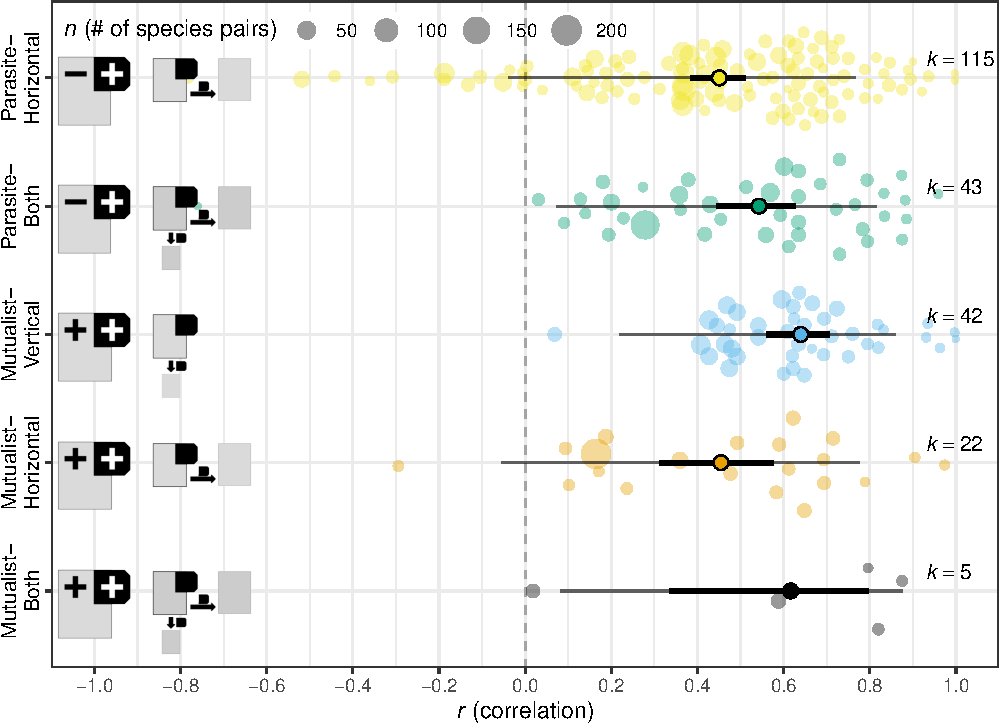
\includegraphics{Supporting_Information_files/figure-latex/unnamed-chunk-37-1.pdf}

\begin{Shaded}
\begin{Highlighting}[]
\CommentTok{## fig 3}
\NormalTok{g <-}\StringTok{ }\KeywordTok{ggplot}\NormalTok{(}\DataTypeTok{data =}\NormalTok{ res_symbiosis_transmission1, }\KeywordTok{aes}\NormalTok{(}\DataTypeTok{x =} \KeywordTok{tanh}\NormalTok{(estimate), }\DataTypeTok{y =}\NormalTok{ name)) }\OperatorTok{+}
\StringTok{  }\KeywordTok{scale_x_continuous}\NormalTok{(}\DataTypeTok{limits=}\KeywordTok{c}\NormalTok{(}\OperatorTok{-}\DecValTok{1}\NormalTok{, }\DecValTok{1}\NormalTok{), }\DataTypeTok{breaks =} \KeywordTok{seq}\NormalTok{(}\OperatorTok{-}\DecValTok{1}\NormalTok{, }\DecValTok{1}\NormalTok{, }\DataTypeTok{by =} \FloatTok{0.2}\NormalTok{) ) }\OperatorTok{+}
\StringTok{  }\KeywordTok{geom_quasirandom}\NormalTok{(}\DataTypeTok{data =}\NormalTok{ dat }\OperatorTok\StringTok{ }\KeywordTok{filter}\NormalTok{(}\OperatorTok{!}\KeywordTok{is.na}\NormalTok{(symbiosis_transmission)), }
                   \KeywordTok{aes}\NormalTok{(}\DataTypeTok{x=} \KeywordTok{tanh}\NormalTok{(Zr), }\DataTypeTok{y =}\NormalTok{ symbiosis_transmission, }\DataTypeTok{size =}\NormalTok{ ((}\DecValTok{1}\OperatorTok{/}\NormalTok{VZr) }\OperatorTok{+}\StringTok{ }\DecValTok{3}\NormalTok{), }\DataTypeTok{colour =}\NormalTok{ symbiosis_transmission), }\DataTypeTok{groupOnX =} \OtherTok{FALSE}\NormalTok{, }\DataTypeTok{alpha=}\FloatTok{0.4}\NormalTok{) }\OperatorTok{+}\StringTok{ }
\StringTok{  }\CommentTok{# 95 %precition interval (PI)}
\StringTok{  }\KeywordTok{geom_errorbarh}\NormalTok{(}\KeywordTok{aes}\NormalTok{(}\DataTypeTok{xmin =} \KeywordTok{tanh}\NormalTok{(lowerPR), }\DataTypeTok{xmax =} \KeywordTok{tanh}\NormalTok{(upperPR)),  }\DataTypeTok{height =} \DecValTok{0}\NormalTok{, }\DataTypeTok{show.legend =}\NormalTok{ F, }\DataTypeTok{size =} \FloatTok{0.5}\NormalTok{, }\DataTypeTok{alpha =} \FloatTok{0.6}\NormalTok{) }\OperatorTok{+}
\StringTok{  }\CommentTok{# 95 %CI}
\StringTok{  }\KeywordTok{geom_errorbarh}\NormalTok{(}\KeywordTok{aes}\NormalTok{(}\DataTypeTok{xmin =} \KeywordTok{tanh}\NormalTok{(lowerCL), }\DataTypeTok{xmax =} \KeywordTok{tanh}\NormalTok{(upperCL)),  }\DataTypeTok{height =} \DecValTok{0}\NormalTok{, }\DataTypeTok{show.legend =}\NormalTok{ F, }\DataTypeTok{size =} \FloatTok{1.2}\NormalTok{) }\OperatorTok{+}
\StringTok{  }\KeywordTok{geom_vline}\NormalTok{(}\DataTypeTok{xintercept =} \DecValTok{0}\NormalTok{, }\DataTypeTok{linetype =} \DecValTok{2}\NormalTok{, }\DataTypeTok{colour =} \StringTok{"black"}\NormalTok{, }\DataTypeTok{alpha =} \FloatTok{0.3}\NormalTok{) }\OperatorTok{+}
\StringTok{  }\CommentTok{# creating dots and different size (bee-swarm and bubbles)}
\StringTok{  }\KeywordTok{geom_point}\NormalTok{(}\KeywordTok{aes}\NormalTok{(}\DataTypeTok{fill =}\NormalTok{ name), }\DataTypeTok{size =} \DecValTok{3}\NormalTok{, }\DataTypeTok{shape =} \DecValTok{21}\NormalTok{) }\OperatorTok{+}\StringTok{ }\CommentTok{#}
\StringTok{  }\CommentTok{# setting colours}
\StringTok{  }\KeywordTok{scale_color_manual}\NormalTok{(}\DataTypeTok{values =}   \KeywordTok{c}\NormalTok{(}\StringTok{"MutualistBoth"}\NormalTok{=}\StringTok{ }\NormalTok{colour_ls[}\DecValTok{1}\NormalTok{], }\StringTok{"MutualistHorizontal"}\NormalTok{=}\StringTok{ }\NormalTok{colour_ls[}\DecValTok{2}\NormalTok{], }\StringTok{"MutualistVertical"}\NormalTok{ =}\StringTok{ }\NormalTok{colour_ls[}\DecValTok{3}\NormalTok{],}\StringTok{"ParasiteBoth"}\NormalTok{=}\StringTok{ }\NormalTok{colour_ls[}\DecValTok{4}\NormalTok{], }\StringTok{"ParasiteHorizontal"}\NormalTok{ =}\StringTok{ }\NormalTok{colour_ls[}\DecValTok{5}\NormalTok{])) }\OperatorTok{+}
\StringTok{  }\KeywordTok{scale_fill_manual}\NormalTok{(}\DataTypeTok{values =} \KeywordTok{c}\NormalTok{(}\StringTok{"MutualistBoth"}\NormalTok{=}\StringTok{ }\NormalTok{colour_ls[}\DecValTok{1}\NormalTok{], }\StringTok{"MutualistHorizontal"}\NormalTok{=}\StringTok{ }\NormalTok{colour_ls[}\DecValTok{2}\NormalTok{], }\StringTok{"MutualistVertical"}\NormalTok{ =}\StringTok{ }\NormalTok{colour_ls[}\DecValTok{3}\NormalTok{],}\StringTok{"ParasiteBoth"}\NormalTok{=}\StringTok{ }\NormalTok{colour_ls[}\DecValTok{4}\NormalTok{], }\StringTok{"ParasiteHorizontal"}\NormalTok{ =}\StringTok{ }\NormalTok{colour_ls[}\DecValTok{5}\NormalTok{])) }\OperatorTok{+}
\StringTok{  }\KeywordTok{scale_y_discrete}\NormalTok{(}\DataTypeTok{labels =} \KeywordTok{c}\NormalTok{(}\StringTok{"MutualistBoth"}\NormalTok{ =}\StringTok{ "Mutualist-}\CharTok{\textbackslash{}n}\StringTok{Both"}\NormalTok{, }\StringTok{"MutualistHorizontal"}\NormalTok{ =}\StringTok{ "Mutualist-}\CharTok{\textbackslash{}n}\StringTok{Horizontal"}\NormalTok{,}\StringTok{"MutualistVertical"}\NormalTok{ =}\StringTok{ "Mutualist-}\CharTok{\textbackslash{}n}\StringTok{Vertical"}\NormalTok{, }\StringTok{"ParasiteBoth"}\NormalTok{ =}\StringTok{ "Parasite-}\CharTok{\textbackslash{}n}\StringTok{Both"}\NormalTok{, }\StringTok{"ParasiteHorizontal"}\NormalTok{ =}\StringTok{ "Parasite-}\CharTok{\textbackslash{}n}\StringTok{Horizontal"}\NormalTok{)) }\OperatorTok{+}
\StringTok{  }\KeywordTok{annotate}\NormalTok{(}\StringTok{'text'}\NormalTok{, }\DataTypeTok{x =} \FloatTok{0.93}\NormalTok{, }\DataTypeTok{y =} \DecValTok{1}\OperatorTok{:}\DecValTok{5} \OperatorTok{+}\StringTok{ }\FloatTok{0.15}\NormalTok{, }\DataTypeTok{label=} \KeywordTok{paste}\NormalTok{(}\StringTok{"italic(k)=="}\NormalTok{, res_symbiosis_transmission1}\OperatorTok{$}\NormalTok{n), }\DataTypeTok{parse=}\OtherTok{TRUE}\NormalTok{, }\DataTypeTok{hjust =} \StringTok{"left"}\NormalTok{, }\DataTypeTok{size=}\FloatTok{3.5}\NormalTok{) }\OperatorTok{+}
\StringTok{  }\KeywordTok{labs}\NormalTok{(}\DataTypeTok{x =} \KeywordTok{expression}\NormalTok{(}\KeywordTok{paste}\NormalTok{(}\KeywordTok{italic}\NormalTok{(r), }\StringTok{" (correlation)"}\NormalTok{)), }\DataTypeTok{y =} \StringTok{""}\NormalTok{, }\DataTypeTok{size =} \KeywordTok{expression}\NormalTok{(}\KeywordTok{paste}\NormalTok{(}\KeywordTok{italic}\NormalTok{(n), }\StringTok{" (# of species pairs)"}\NormalTok{)) ,}\DataTypeTok{tag =} \StringTok{"g"}\NormalTok{ ) }\OperatorTok{+}
\StringTok{  }\KeywordTok{guides}\NormalTok{(}\DataTypeTok{fill =} \StringTok{"none"}\NormalTok{, }\DataTypeTok{colour =} \StringTok{"none"}\NormalTok{) }\OperatorTok{+}
\StringTok{  }\KeywordTok{theme_bw}\NormalTok{() }\OperatorTok{+}
\StringTok{  }\KeywordTok{theme}\NormalTok{(}\DataTypeTok{legend.position=}\StringTok{"none"}\NormalTok{) }\OperatorTok{+}
\StringTok{  }\KeywordTok{theme}\NormalTok{(}\DataTypeTok{axis.text.y =} \KeywordTok{element_text}\NormalTok{(}\DataTypeTok{size =} \DecValTok{10}\NormalTok{, }\DataTypeTok{colour =}\StringTok{"black"}\NormalTok{,}\DataTypeTok{hjust =} \FloatTok{0.5}\NormalTok{, }\DataTypeTok{angle =} \DecValTok{90}\NormalTok{)) }\OperatorTok{+}
\StringTok{  }\CommentTok{# putting pictures in}
\StringTok{  }\KeywordTok{annotation_custom}\NormalTok{(}\KeywordTok{rasterGrob}\NormalTok{(image_mutualism), }\DataTypeTok{xmin =} \FloatTok{-1.1}\NormalTok{, }\DataTypeTok{xmax =} \FloatTok{-0.9}\NormalTok{, }\DataTypeTok{ymin =} \FloatTok{0.6}\NormalTok{, }\DataTypeTok{ymax =} \FloatTok{1.2}\NormalTok{) }\OperatorTok{+}\StringTok{ }
\StringTok{  }\KeywordTok{annotation_custom}\NormalTok{(}\KeywordTok{rasterGrob}\NormalTok{(image_both), }\DataTypeTok{xmin =} \FloatTok{-0.9}\NormalTok{, }\DataTypeTok{xmax =} \FloatTok{-0.6}\NormalTok{, }\DataTypeTok{ymin =} \FloatTok{0.4}\NormalTok{, }\DataTypeTok{ymax =} \FloatTok{1.2}\NormalTok{) }\OperatorTok{+}\StringTok{ }
\StringTok{  }\KeywordTok{annotation_custom}\NormalTok{(}\KeywordTok{rasterGrob}\NormalTok{(image_mutualism), }\DataTypeTok{xmin =} \FloatTok{-1.1}\NormalTok{, }\DataTypeTok{xmax =} \FloatTok{-0.9}\NormalTok{, }\DataTypeTok{ymin =} \FloatTok{1.6}\NormalTok{, }\DataTypeTok{ymax =} \FloatTok{2.2}\NormalTok{) }\OperatorTok{+}
\StringTok{  }\KeywordTok{annotation_custom}\NormalTok{(}\KeywordTok{rasterGrob}\NormalTok{(image_horizontal),}\DataTypeTok{xmin =} \FloatTok{-0.9}\NormalTok{, }\DataTypeTok{xmax =} \FloatTok{-0.6}\NormalTok{, }\DataTypeTok{ymin =} \FloatTok{1.4}\NormalTok{, }\DataTypeTok{ymax =} \FloatTok{2.2}\NormalTok{) }\OperatorTok{+}
\StringTok{  }\KeywordTok{annotation_custom}\NormalTok{(}\KeywordTok{rasterGrob}\NormalTok{(image_mutualism), }\DataTypeTok{xmin =} \FloatTok{-1.1}\NormalTok{, }\DataTypeTok{xmax =} \FloatTok{-0.9}\NormalTok{, }\DataTypeTok{ymin =} \FloatTok{2.6}\NormalTok{, }\DataTypeTok{ymax =} \FloatTok{3.2}\NormalTok{) }\OperatorTok{+}\StringTok{ }
\StringTok{  }\KeywordTok{annotation_custom}\NormalTok{(}\KeywordTok{rasterGrob}\NormalTok{(image_vertical), }\DataTypeTok{xmin =} \FloatTok{-0.9}\NormalTok{, }\DataTypeTok{xmax =} \FloatTok{-0.6}\NormalTok{, }\DataTypeTok{ymin =} \FloatTok{2.4}\NormalTok{, }\DataTypeTok{ymax =} \FloatTok{3.2}\NormalTok{) }\OperatorTok{+}\StringTok{ }
\StringTok{  }\KeywordTok{annotation_custom}\NormalTok{(}\KeywordTok{rasterGrob}\NormalTok{(image_parasitism), }\DataTypeTok{xmin =} \FloatTok{-1.1}\NormalTok{, }\DataTypeTok{xmax =} \FloatTok{-0.9}\NormalTok{, }\DataTypeTok{ymin =} \FloatTok{3.6}\NormalTok{, }\DataTypeTok{ymax =} \FloatTok{4.2}\NormalTok{) }\OperatorTok{+}
\StringTok{  }\KeywordTok{annotation_custom}\NormalTok{(}\KeywordTok{rasterGrob}\NormalTok{(image_both), }\DataTypeTok{xmin =} \FloatTok{-0.9}\NormalTok{, }\DataTypeTok{xmax =} \FloatTok{-0.6}\NormalTok{, }\DataTypeTok{ymin =} \FloatTok{3.4}\NormalTok{, }\DataTypeTok{ymax =} \FloatTok{4.2}\NormalTok{) }\OperatorTok{+}
\StringTok{  }\KeywordTok{annotation_custom}\NormalTok{(}\KeywordTok{rasterGrob}\NormalTok{(image_parasitism), }\DataTypeTok{xmin =} \FloatTok{-1.1}\NormalTok{, }\DataTypeTok{xmax =} \FloatTok{-0.9}\NormalTok{, }\DataTypeTok{ymin =} \FloatTok{4.6}\NormalTok{, }\DataTypeTok{ymax =} \FloatTok{5.2}\NormalTok{) }\OperatorTok{+}
\StringTok{  }\KeywordTok{annotation_custom}\NormalTok{(}\KeywordTok{rasterGrob}\NormalTok{(image_horizontal), }\DataTypeTok{xmin =} \FloatTok{-0.9}\NormalTok{, }\DataTypeTok{xmax =} \FloatTok{-0.6}\NormalTok{, }\DataTypeTok{ymin =} \FloatTok{4.4}\NormalTok{, }\DataTypeTok{ymax =} \FloatTok{5.2}\NormalTok{)}
\end{Highlighting}
\end{Shaded}

\textbf{Figure 3g:} A forest plot showing the group-wise means (the
categorical variable \texttt{symbiosis\_transmission}) with their 95\%
confidence intervals (thick lines) and 95\% prediction intervals (thin
lines), with observed effect sizes based on various sample sizes.

\hypertarget{putting-together-figure-3}{%
\paragraph{Putting together Figure 3}\label{putting-together-figure-3}}

\begin{Shaded}
\begin{Highlighting}[]
\CommentTok{# building fig 3 using patchwork}
\NormalTok{fig3 <-}\StringTok{ }\NormalTok{(a}\OperatorTok{/}\NormalTok{b}\OperatorTok{/}\NormalTok{c}\OperatorTok{/}\NormalTok{d }\OperatorTok{+}\StringTok{ }\KeywordTok{plot_layout}\NormalTok{(}\DataTypeTok{heights =} \KeywordTok{c}\NormalTok{(}\FloatTok{1.6}\NormalTok{, }\DecValTok{2}\NormalTok{, }\FloatTok{3.7}\NormalTok{, }\FloatTok{3.7}\NormalTok{))) }\OperatorTok{|}\StringTok{ }\NormalTok{(e}\OperatorTok{/}\NormalTok{f}\OperatorTok{/}\NormalTok{g }\OperatorTok{+}\StringTok{ }\KeywordTok{plot_layout}\NormalTok{(}\DataTypeTok{heights =} \KeywordTok{c}\NormalTok{(}\FloatTok{2.8}\NormalTok{, }
    \FloatTok{2.8}\NormalTok{, }\FloatTok{4.4}\NormalTok{)))  }\CommentTok{#+ plot_annotation(tag_levels = 'a', tag_suffix = ')')}

\NormalTok{fig3}
\end{Highlighting}
\end{Shaded}

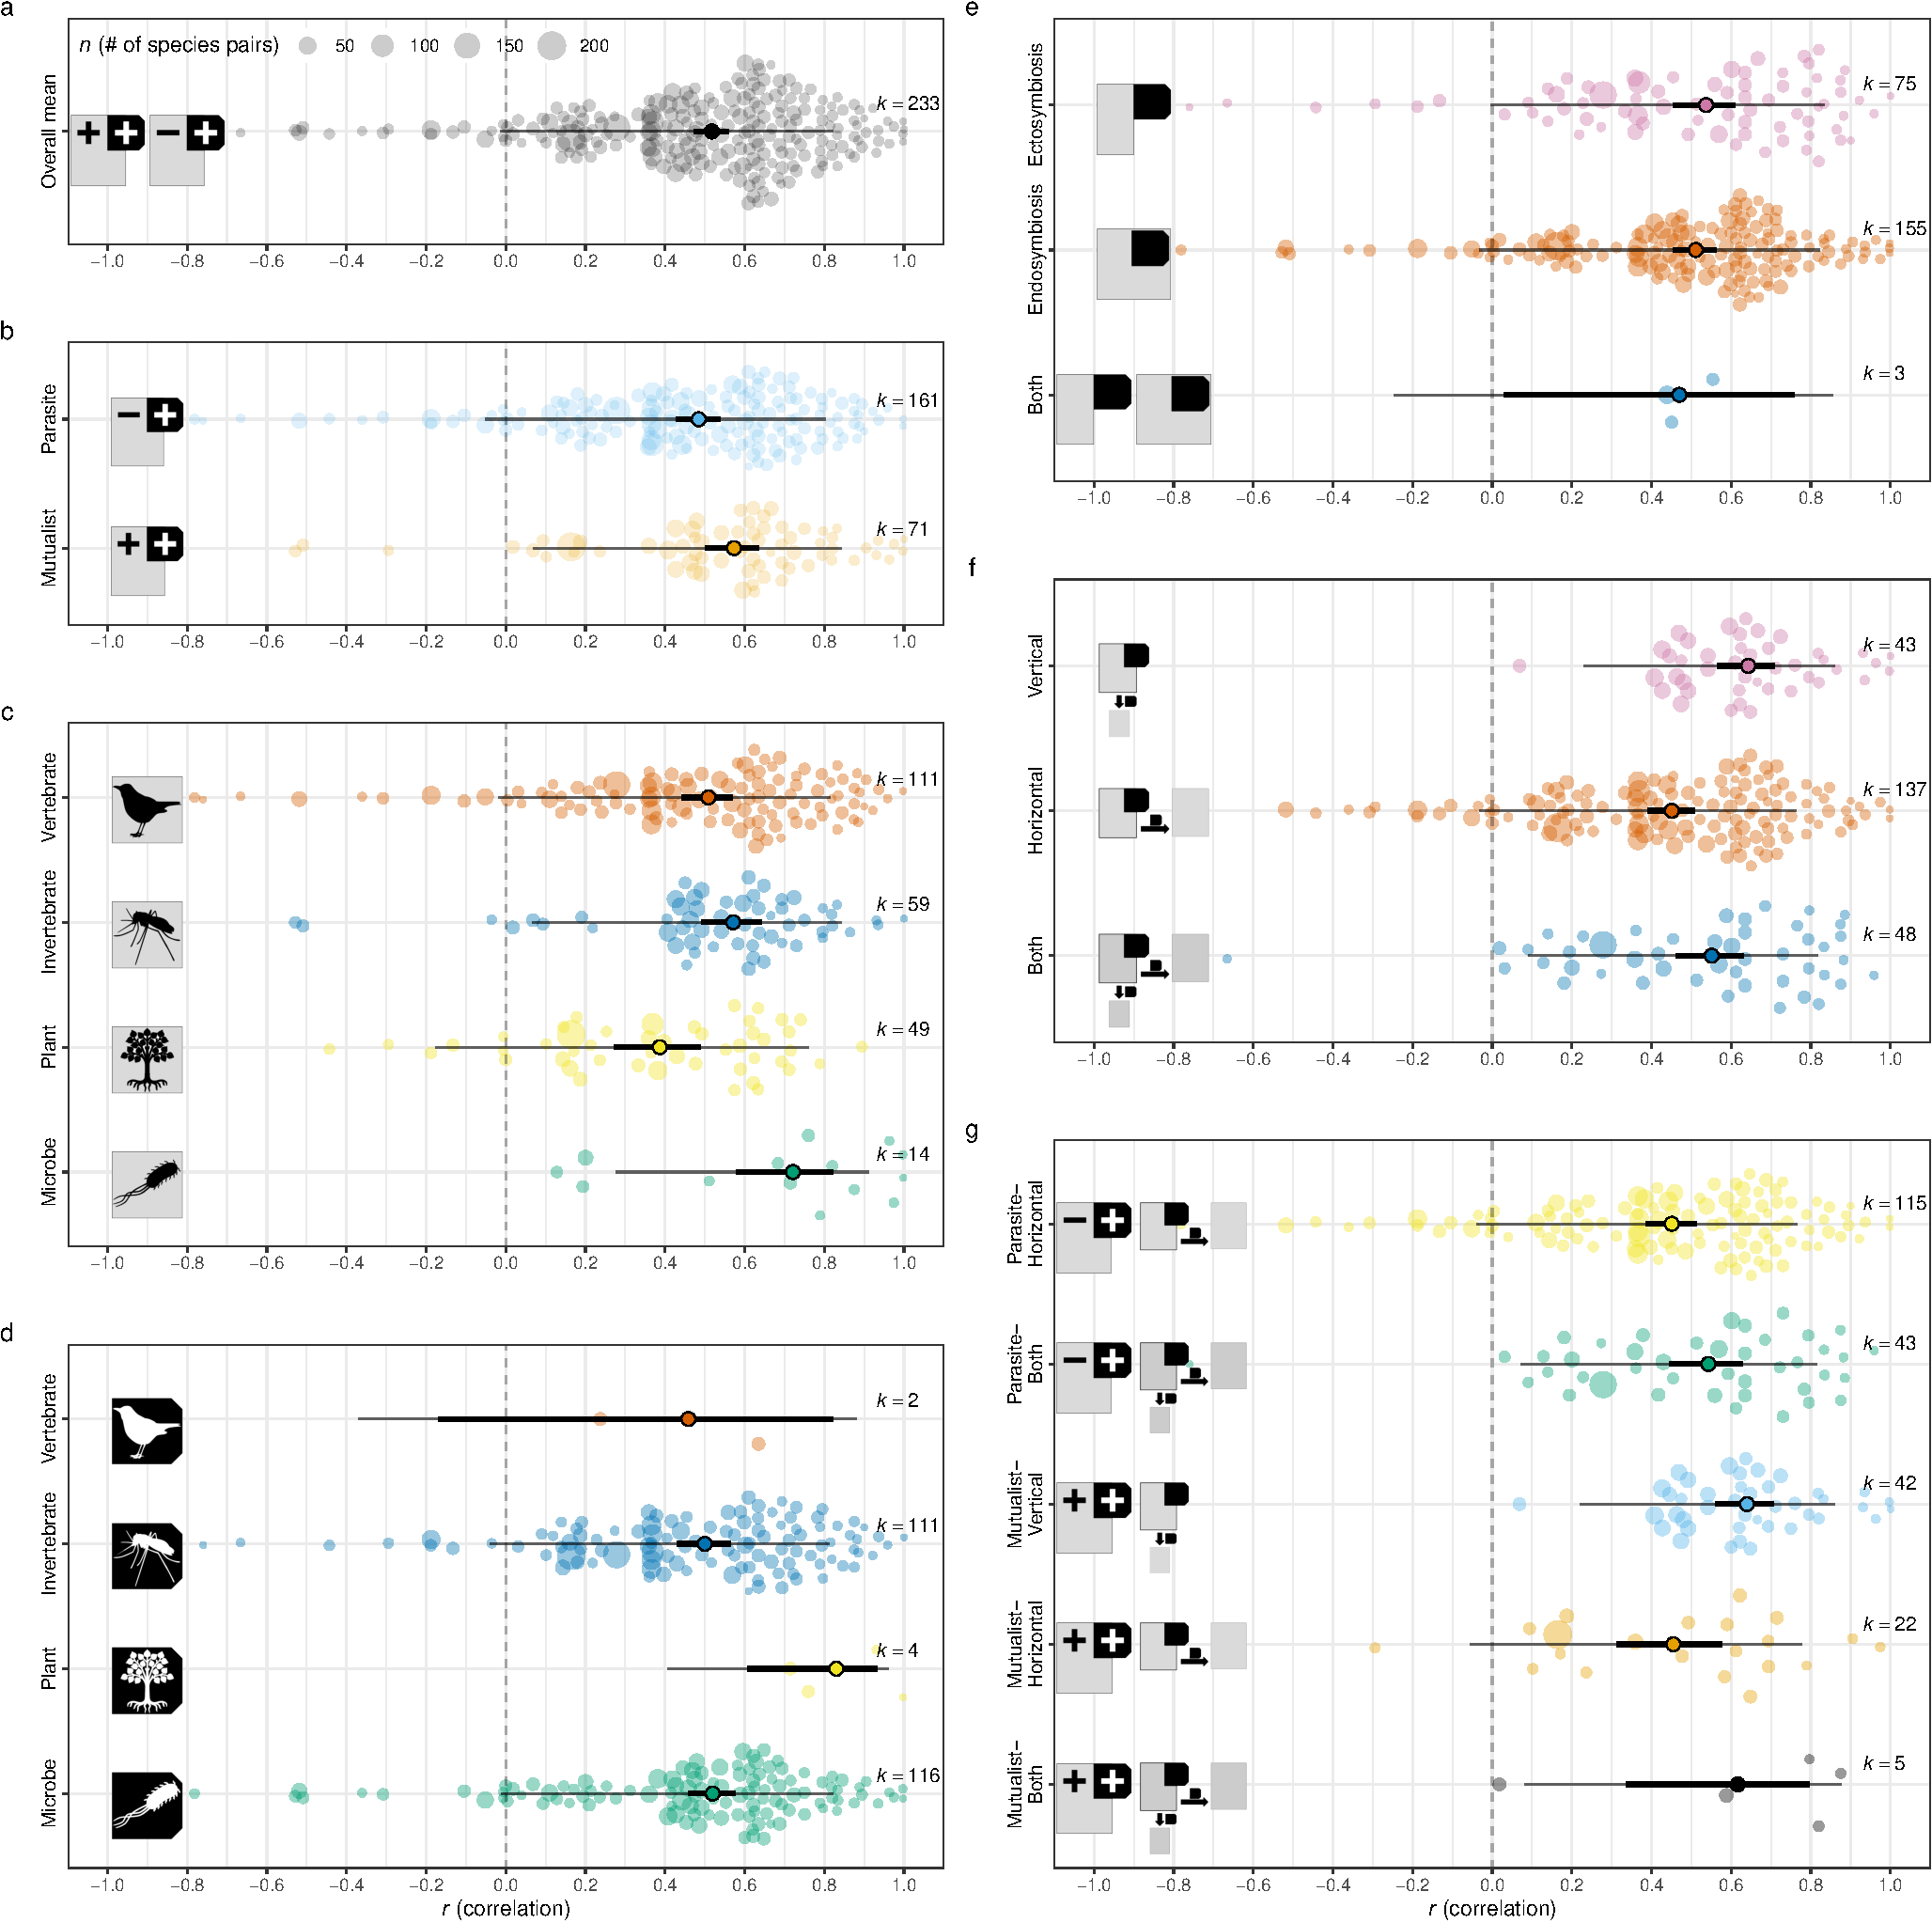
\includegraphics{Supporting_Information_files/figure-latex/unnamed-chunk-38-1.pdf}

\begin{Shaded}
\begin{Highlighting}[]
\CommentTok{# ggsave('../figs/fig3.png', width = 14, height = 14) ggsave('../figs/fig3.pdf',}
\CommentTok{# width = 14, height = 14)}
\end{Highlighting}
\end{Shaded}

\textbf{Figure 3:} putting all 7 panels together: Figure 3a - Figure 3g
(see the main text)

\hypertarget{additional-analyses-uni-predictor}{%
\subsubsection{Additional analyses
(uni-predictor)}\label{additional-analyses-uni-predictor}}

These are extra analyses not discussed in the main text.

\hypertarget{the-combined-effect-of-host-taxa-and-symbiosis-parasitism-vs.-mutualism}{%
\paragraph{The combined effect of host taxa and symbiosis (parasitism
vs.~mutualism)}\label{the-combined-effect-of-host-taxa-and-symbiosis-parasitism-vs.-mutualism}}

\begin{Shaded}
\begin{Highlighting}[]
\CommentTok{# reordering}
\NormalTok{dat}\OperatorTok{$}\NormalTok{host_tax_symbiosis <-}\StringTok{ }\KeywordTok{factor}\NormalTok{(dat}\OperatorTok{$}\NormalTok{host_tax_symbiosis, }\DataTypeTok{levels =} \KeywordTok{c}\NormalTok{(}\StringTok{"MicrobeMutualist"}\NormalTok{, }
    \StringTok{"MicrobeParasite"}\NormalTok{, }\StringTok{"PlantMutualist"}\NormalTok{, }\StringTok{"PlantParasite"}\NormalTok{, }\StringTok{"InvertMutualist"}\NormalTok{, }\StringTok{"InvertParasite"}\NormalTok{, }
    \StringTok{"VertMutualist"}\NormalTok{, }\StringTok{"VertParasite"}\NormalTok{))}

\CommentTok{# meta-regression: mutiple intercepts}
\NormalTok{mr_host_tax_symbiosis1 <-}\StringTok{ }\KeywordTok{rma.mv}\NormalTok{(}\DataTypeTok{yi =}\NormalTok{ Zr, }\DataTypeTok{V =}\NormalTok{ VZr, }\DataTypeTok{mods =} \OperatorTok{~}\NormalTok{host_tax_symbiosis }\OperatorTok{-}\StringTok{ }\DecValTok{1}\NormalTok{, }
    \DataTypeTok{test =} \StringTok{"t"}\NormalTok{, }\DataTypeTok{random =} \OperatorTok{~}\DecValTok{1} \OperatorTok{|}\StringTok{ }\NormalTok{authors, }\DataTypeTok{data =}\NormalTok{ dat)}

\CommentTok{# # meta-regression: contrasts x 10 getting the level names out}
\NormalTok{level_names <-}\StringTok{ }\KeywordTok{levels}\NormalTok{(dat}\OperatorTok{$}\NormalTok{host_tax_symbiosis)}

\CommentTok{# helper function to run metafor meta-regression}
\NormalTok{run_rma <-}\StringTok{ }\ControlFlowTok{function}\NormalTok{(name) \{}
    \KeywordTok{rma.mv}\NormalTok{(}\DataTypeTok{yi =}\NormalTok{ Zr, }\DataTypeTok{V =}\NormalTok{ VZr, }\DataTypeTok{mods =} \OperatorTok{~}\KeywordTok{relevel}\NormalTok{(host_tax_symbiosis, }\DataTypeTok{ref =}\NormalTok{ name), }\DataTypeTok{test =} \StringTok{"t"}\NormalTok{, }
        \DataTypeTok{random =} \OperatorTok{~}\DecValTok{1} \OperatorTok{|}\StringTok{ }\NormalTok{authors, }\DataTypeTok{data =}\NormalTok{ dat)}
\NormalTok{\}}

\CommentTok{# results of meta-regression including all contrast results; taking the last}
\CommentTok{# level out ([-length(level_names)])}
\NormalTok{mr_host_tax_symbiosis <-}\StringTok{ }\KeywordTok{map}\NormalTok{(level_names[}\OperatorTok{-}\KeywordTok{length}\NormalTok{(level_names)], run_rma)}
\end{Highlighting}
\end{Shaded}

\textbf{Supplementary Table 10:} Regression coefficients (Estimate),
95\% confidence intervals (CIs), variance components (V) and variance
explained, \emph{R}\textsuperscript{2}\textsubscript{{[}marginal{]}}
(R2) from the meta-regression with \texttt{host\_tax\_symbiosis}.

\begin{Shaded}
\begin{Highlighting}[]
\CommentTok{# getting marginal R2}
\NormalTok{r2_host_tax_symbiosis1 <-}\StringTok{ }\KeywordTok{R2}\NormalTok{(mr_host_tax_symbiosis1)}

\CommentTok{# getting estimates}
\NormalTok{res_host_tax_symbiosis1 <-}\StringTok{ }\KeywordTok{get_est}\NormalTok{(mr_host_tax_symbiosis1, }\DataTypeTok{mod =} \StringTok{"host_tax_symbiosis"}\NormalTok{)}
\NormalTok{res_host_tax_symbiosis <-}\StringTok{ }\KeywordTok{map}\NormalTok{(mr_host_tax_symbiosis, }\OperatorTok{~}\KeywordTok{get_est}\NormalTok{(.x, }\DataTypeTok{mod =} \StringTok{"host_tax_symbiosis"}\NormalTok{))}

\CommentTok{# a list of the numbers to take out unnecessary contrasts}
\NormalTok{contra_list <-}\StringTok{ }\KeywordTok{Map}\NormalTok{(seq, }\DataTypeTok{from =} \DecValTok{1}\NormalTok{, }\DataTypeTok{to =} \DecValTok{1}\OperatorTok{:}\DecValTok{7}\NormalTok{)}

\CommentTok{# you need to flatten twice: first to make it a list and make it a vector}
\NormalTok{estimates <-}\StringTok{ }\KeywordTok{map2}\NormalTok{(res_host_tax_symbiosis, contra_list, }\OperatorTok{~}\NormalTok{.x[}\OperatorTok{-}\NormalTok{(.y), }\StringTok{"estimate"}\NormalTok{]) }\OperatorTok\StringTok{ }
\StringTok{    }\KeywordTok{flatten}\NormalTok{() }\OperatorTok\StringTok{ }\KeywordTok{flatten_dbl}\NormalTok{()}
\NormalTok{lowerCLs <-}\StringTok{ }\KeywordTok{map2}\NormalTok{(res_host_tax_symbiosis, contra_list, }\OperatorTok{~}\NormalTok{.x[}\OperatorTok{-}\NormalTok{(.y), }\StringTok{"lowerCL"}\NormalTok{]) }\OperatorTok\StringTok{ }
\StringTok{    }\KeywordTok{flatten}\NormalTok{() }\OperatorTok\StringTok{ }\KeywordTok{flatten_dbl}\NormalTok{()}
\NormalTok{upperCLs <-}\StringTok{ }\KeywordTok{map2}\NormalTok{(res_host_tax_symbiosis, contra_list, }\OperatorTok{~}\NormalTok{.x[}\OperatorTok{-}\NormalTok{(.y), }\StringTok{"upperCL"}\NormalTok{]) }\OperatorTok\StringTok{ }
\StringTok{    }\KeywordTok{flatten}\NormalTok{() }\OperatorTok\StringTok{ }\KeywordTok{flatten_dbl}\NormalTok{()}

\CommentTok{# creating a table}
\KeywordTok{tibble}\NormalTok{(}\StringTok{`}\DataTypeTok{Fixed effect}\StringTok{`}\NormalTok{ =}\StringTok{ }\KeywordTok{c}\NormalTok{(}\KeywordTok{as.character}\NormalTok{(res_host_tax_symbiosis1}\OperatorTok{$}\NormalTok{name), }\KeywordTok{cont_gen}\NormalTok{(res_host_tax_symbiosis1}\OperatorTok{$}\NormalTok{name)), }
    \DataTypeTok{Estimate =} \KeywordTok{c}\NormalTok{(res_host_tax_symbiosis1}\OperatorTok{$}\NormalTok{estimate, estimates), }\StringTok{`}\DataTypeTok{Lower CI [0.025]}\StringTok{`}\NormalTok{ =}\StringTok{ }\KeywordTok{c}\NormalTok{(res_host_tax_symbiosis1}\OperatorTok{$}\NormalTok{lowerCL, }
\NormalTok{        lowerCLs), }\StringTok{`}\DataTypeTok{Upper CI  [0.975]}\StringTok{`}\NormalTok{ =}\StringTok{ }\KeywordTok{c}\NormalTok{(res_host_tax_symbiosis1}\OperatorTok{$}\NormalTok{upperCL, upperCLs), }
    \StringTok{`}\DataTypeTok{V[authors]}\StringTok{`}\NormalTok{ =}\StringTok{ }\KeywordTok{c}\NormalTok{(mr_host_tax_symbiosis1}\OperatorTok{$}\NormalTok{sigma2, }\KeywordTok{rep}\NormalTok{(}\OtherTok{NA}\NormalTok{, (}\DecValTok{8} \OperatorTok{+}\StringTok{ }\KeywordTok{choose}\NormalTok{(}\DecValTok{8}\NormalTok{, }\DecValTok{2}\NormalTok{)) }\OperatorTok{-}\StringTok{ }
\StringTok{        }\DecValTok{1}\NormalTok{)), }\DataTypeTok{R2 =} \KeywordTok{c}\NormalTok{(r2_host_tax_symbiosis1[}\DecValTok{1}\NormalTok{], }\KeywordTok{rep}\NormalTok{(}\OtherTok{NA}\NormalTok{, (}\DecValTok{8} \OperatorTok{+}\StringTok{ }\KeywordTok{choose}\NormalTok{(}\DecValTok{8}\NormalTok{, }\DecValTok{2}\NormalTok{)) }\OperatorTok{-}\StringTok{ }\DecValTok{1}\NormalTok{))) }\OperatorTok\StringTok{ }
\StringTok{    }\KeywordTok{kable}\NormalTok{(}\StringTok{"html"}\NormalTok{, }\DataTypeTok{digits =} \DecValTok{3}\NormalTok{) }\OperatorTok\StringTok{ }\KeywordTok{kable_styling}\NormalTok{(}\StringTok{"striped"}\NormalTok{, }\DataTypeTok{position =} \StringTok{"left"}\NormalTok{) }\OperatorTok\StringTok{ }
\StringTok{    }\KeywordTok{scroll_box}\NormalTok{(}\DataTypeTok{width =} \StringTok{"100%"}\NormalTok{, }\DataTypeTok{height =} \StringTok{"300px"}\NormalTok{)}
\end{Highlighting}
\end{Shaded}

Fixed effect

Estimate

Lower CI {[}0.025{]}

Upper CI {[}0.975{]}

V{[}authors{]}

R2

MicrobeMutualist

1.348

1.006

1.689

0.074

0.302

MicrobeParasite

0.435

0.088

0.782

NA

NA

PlantMutualist

0.401

0.217

0.585

NA

NA

PlantParasite

0.412

0.262

0.562

NA

NA

InvertMutualist

0.647

0.525

0.768

NA

NA

InvertParasite

0.604

0.371

0.837

NA

NA

VertMutualist

1.499

0.467

2.531

NA

NA

VertParasite

0.550

0.467

0.633

NA

NA

MicrobeMutualist-MicrobeParasite

-0.913

-1.400

-0.426

NA

NA

MicrobeMutualist-PlantMutualist

-0.947

-1.335

-0.559

NA

NA

MicrobeMutualist-PlantParasite

-0.936

-1.309

-0.563

NA

NA

MicrobeMutualist-InvertMutualist

-0.701

-1.063

-0.338

NA

NA

MicrobeMutualist-InvertParasite

-0.743

-1.157

-0.330

NA

NA

MicrobeMutualist-VertMutualist

0.151

-0.936

1.238

NA

NA

MicrobeMutualist-VertParasite

-0.798

-1.149

-0.446

NA

NA

MicrobeParasite-PlantMutualist

-0.034

-0.426

0.359

NA

NA

MicrobeParasite-PlantParasite

-0.023

-0.401

0.355

NA

NA

MicrobeParasite-InvertMutualist

0.212

-0.155

0.580

NA

NA

MicrobeParasite-InvertParasite

0.170

-0.248

0.587

NA

NA

MicrobeParasite-VertMutualist

1.064

-0.025

2.153

NA

NA

MicrobeParasite-VertParasite

0.115

-0.241

0.472

NA

NA

PlantMutualist-PlantParasite

0.011

-0.211

0.233

NA

NA

PlantMutualist-InvertMutualist

0.246

0.026

0.466

NA

NA

PlantMutualist-InvertParasite

0.203

-0.094

0.500

NA

NA

PlantMutualist-VertMutualist

1.098

0.049

2.146

NA

NA

PlantMutualist-VertParasite

0.149

-0.053

0.351

NA

NA

PlantParasite-InvertMutualist

0.235

0.042

0.428

NA

NA

PlantParasite-InvertParasite

0.192

-0.085

0.469

NA

NA

PlantParasite-VertMutualist

1.087

0.044

2.129

NA

NA

PlantParasite-VertParasite

0.138

-0.033

0.309

NA

NA

InvertMutualist-InvertParasite

-0.043

-0.306

0.220

NA

NA

InvertMutualist-VertMutualist

0.852

-0.187

1.891

NA

NA

InvertMutualist-VertParasite

-0.097

-0.244

0.050

NA

NA

InvertParasite-VertMutualist

0.894

-0.164

1.952

NA

NA

InvertParasite-VertParasite

-0.054

-0.295

0.187

NA

NA

VertMutualist-VertParasite

-0.949

-1.984

0.087

NA

NA

\begin{Shaded}
\begin{Highlighting}[]
\CommentTok{# adding sample size (k) for each category}
\NormalTok{k_host_tax_symbiosis <-}\StringTok{ }\NormalTok{dat }\OperatorTok\StringTok{ }\KeywordTok{group_by}\NormalTok{(host_tax_symbiosis) }\OperatorTok\StringTok{ }\KeywordTok{count}\NormalTok{()}
\CommentTok{# getting estimates and predicitons}
\NormalTok{pred_host_tax_symbiosis <-}\StringTok{ }\KeywordTok{get_pred}\NormalTok{(mr_host_tax_symbiosis1, }\DataTypeTok{mod =} \StringTok{"host_tax_symbiosis"}\NormalTok{) }
\NormalTok{res_host_tax_symbiosis1 <-}\StringTok{ }\KeywordTok{left_join}\NormalTok{(res_host_tax_symbiosis1, k_host_tax_symbiosis, }\DataTypeTok{by =}  \KeywordTok{c}\NormalTok{(}\StringTok{"name"}\NormalTok{ =}\StringTok{ "host_tax_symbiosis"}\NormalTok{))  }\OperatorTok\StringTok{ }\KeywordTok{left_join}\NormalTok{(pred_host_tax_symbiosis)}
\CommentTok{#res_symbiosis1 }
\CommentTok{# drawing a funnel plot - fig 2b}
\NormalTok{fig_host_tax_symbiosis <-}\StringTok{ }\KeywordTok{ggplot}\NormalTok{(}\DataTypeTok{data =}\NormalTok{ res_host_tax_symbiosis1, }\KeywordTok{aes}\NormalTok{(}\DataTypeTok{x =} \KeywordTok{tanh}\NormalTok{(estimate), }\DataTypeTok{y =}\NormalTok{ name)) }\OperatorTok{+}
\StringTok{  }\KeywordTok{scale_x_continuous}\NormalTok{(}\DataTypeTok{limits=}\KeywordTok{c}\NormalTok{(}\OperatorTok{-}\DecValTok{1}\NormalTok{, }\DecValTok{1}\NormalTok{), }\DataTypeTok{breaks =} \KeywordTok{seq}\NormalTok{(}\OperatorTok{-}\DecValTok{1}\NormalTok{, }\DecValTok{1}\NormalTok{, }\DataTypeTok{by =} \FloatTok{0.2}\NormalTok{) ) }\OperatorTok{+}
\StringTok{  }\KeywordTok{geom_quasirandom}\NormalTok{(}\DataTypeTok{data =}\NormalTok{ dat }\OperatorTok\StringTok{ }\KeywordTok{filter}\NormalTok{(}\OperatorTok{!}\KeywordTok{is.na}\NormalTok{(host_tax_symbiosis)), }
                   \KeywordTok{aes}\NormalTok{(}\DataTypeTok{x=} \KeywordTok{tanh}\NormalTok{(Zr), }\DataTypeTok{y =}\NormalTok{ host_tax_symbiosis, }\DataTypeTok{size =}\NormalTok{ ((}\DecValTok{1}\OperatorTok{/}\NormalTok{VZr) }\OperatorTok{+}\StringTok{ }\DecValTok{3}\NormalTok{), }\DataTypeTok{colour =}\NormalTok{ host_tax_symbiosis), }\DataTypeTok{groupOnX =} \OtherTok{FALSE}\NormalTok{, }\DataTypeTok{alpha=}\FloatTok{0.4}\NormalTok{) }\OperatorTok{+}\StringTok{ }
\StringTok{  }\CommentTok{# 95 %precition interval (PI)}
\StringTok{  }\KeywordTok{geom_errorbarh}\NormalTok{(}\KeywordTok{aes}\NormalTok{(}\DataTypeTok{xmin =} \KeywordTok{tanh}\NormalTok{(lowerPR), }\DataTypeTok{xmax =} \KeywordTok{tanh}\NormalTok{(upperPR)),  }\DataTypeTok{height =} \DecValTok{0}\NormalTok{, }\DataTypeTok{show.legend =}\NormalTok{ F, }\DataTypeTok{size =} \FloatTok{0.5}\NormalTok{, }\DataTypeTok{alpha =} \FloatTok{0.6}\NormalTok{) }\OperatorTok{+}
\StringTok{  }\CommentTok{# 95 %CI}
\StringTok{  }\KeywordTok{geom_errorbarh}\NormalTok{(}\KeywordTok{aes}\NormalTok{(}\DataTypeTok{xmin =} \KeywordTok{tanh}\NormalTok{(lowerCL), }\DataTypeTok{xmax =} \KeywordTok{tanh}\NormalTok{(upperCL)),  }\DataTypeTok{height =} \DecValTok{0}\NormalTok{, }\DataTypeTok{show.legend =}\NormalTok{ F, }\DataTypeTok{size =} \FloatTok{1.2}\NormalTok{) }\OperatorTok{+}
\StringTok{  }\KeywordTok{geom_vline}\NormalTok{(}\DataTypeTok{xintercept =} \DecValTok{0}\NormalTok{, }\DataTypeTok{linetype =} \DecValTok{2}\NormalTok{, }\DataTypeTok{colour =} \StringTok{"black"}\NormalTok{, }\DataTypeTok{alpha =} \FloatTok{0.3}\NormalTok{) }\OperatorTok{+}
\StringTok{  }\CommentTok{# creating dots and different size (bee-swarm and bubbles)}
\StringTok{  }\KeywordTok{geom_point}\NormalTok{(}\KeywordTok{aes}\NormalTok{(}\DataTypeTok{fill =}\NormalTok{ name), }\DataTypeTok{size =} \DecValTok{3}\NormalTok{, }\DataTypeTok{shape =} \DecValTok{21}\NormalTok{) }\OperatorTok{+}\StringTok{ }\CommentTok{#}
\StringTok{  }\CommentTok{# setting colours}
\StringTok{  }\KeywordTok{scale_color_manual}\NormalTok{(}\DataTypeTok{values =}   \KeywordTok{c}\NormalTok{(}\StringTok{"MicrobeMutualist"}\NormalTok{=}\StringTok{ }\NormalTok{colour_ls[}\DecValTok{1}\NormalTok{], }\StringTok{"MicrobeParasite"}\NormalTok{=}\StringTok{ }\NormalTok{colour_ls[}\DecValTok{2}\NormalTok{],  }\StringTok{"PlantMutualist"}\NormalTok{=}\StringTok{ }\NormalTok{colour_ls[}\DecValTok{3}\NormalTok{], }\StringTok{"PlantParasite"}\NormalTok{=}\StringTok{ }\NormalTok{colour_ls[}\DecValTok{4}\NormalTok{], }\StringTok{"InvertMutualist"}\NormalTok{ =}\StringTok{ }\NormalTok{colour_ls[}\DecValTok{5}\NormalTok{],  }\StringTok{"InvertParasite"}\NormalTok{=}\StringTok{ }\NormalTok{colour_ls[}\DecValTok{6}\NormalTok{], }\StringTok{"VertMutualist"}\NormalTok{=}\StringTok{ }\NormalTok{colour_ls[}\DecValTok{7}\NormalTok{],     }\StringTok{"VertParasite"}\NormalTok{=}\StringTok{ }\NormalTok{colour_ls[}\DecValTok{8}\NormalTok{] )) }\OperatorTok{+}
\StringTok{  }\KeywordTok{scale_fill_manual}\NormalTok{(}\DataTypeTok{values =} \KeywordTok{c}\NormalTok{(}\StringTok{"MicrobeMutualist"}\NormalTok{=}\StringTok{ }\NormalTok{colour_ls[}\DecValTok{1}\NormalTok{], }\StringTok{"MicrobeParasite"}\NormalTok{=}\StringTok{ }\NormalTok{colour_ls[}\DecValTok{2}\NormalTok{],  }\StringTok{"PlantMutualist"}\NormalTok{=}\StringTok{ }\NormalTok{colour_ls[}\DecValTok{3}\NormalTok{], }\StringTok{"PlantParasite"}\NormalTok{=}\StringTok{ }\NormalTok{colour_ls[}\DecValTok{4}\NormalTok{], }\StringTok{"InvertMutualist"}\NormalTok{ =}\StringTok{ }\NormalTok{colour_ls[}\DecValTok{5}\NormalTok{],  }\StringTok{"InvertParasite"}\NormalTok{=}\StringTok{ }\NormalTok{colour_ls[}\DecValTok{6}\NormalTok{], }\StringTok{"VertMutualist"}\NormalTok{=}\StringTok{ }\NormalTok{colour_ls[}\DecValTok{7}\NormalTok{],     }\StringTok{"VertParasite"}\NormalTok{=}\StringTok{ }\NormalTok{colour_ls[}\DecValTok{8}\NormalTok{] )) }\OperatorTok{+}
\StringTok{  }\KeywordTok{scale_y_discrete}\NormalTok{(}\DataTypeTok{labels =} \KeywordTok{c}\NormalTok{(}\StringTok{"MicrobeMutualist"}\NormalTok{=}\StringTok{ "Microbe-}\CharTok{\textbackslash{}n}\StringTok{Mutualist"}\NormalTok{, }\StringTok{"MicrobeParasite"}\NormalTok{=}\StringTok{ "Microbe-}\CharTok{\textbackslash{}n}\StringTok{Parasite"}\NormalTok{,  }\StringTok{"PlantMutualist"}\NormalTok{ =}\StringTok{ "Plant-}\CharTok{\textbackslash{}n}\StringTok{Mutualist"}\NormalTok{, }\StringTok{"PlantParasite"}\NormalTok{=}\StringTok{"Plant-}\CharTok{\textbackslash{}n}\StringTok{Parasite"}\NormalTok{, }\StringTok{"InvertMutualist"}\NormalTok{ =}\StringTok{ "Invertebrate-}\CharTok{\textbackslash{}n}\StringTok{Mutualist"}\NormalTok{,   }\StringTok{"InvertParasite"}\NormalTok{=}\StringTok{ "Invertebrate-}\CharTok{\textbackslash{}n}\StringTok{Parasite"}\NormalTok{, }\StringTok{"VertMutualist"}\NormalTok{=}\StringTok{ "Vertebrate-}\CharTok{\textbackslash{}n}\StringTok{Mutualist"}\NormalTok{,  }\StringTok{"VertParasite"}\NormalTok{=}\StringTok{ "Vertebrate-}\CharTok{\textbackslash{}n}\StringTok{Parasite"}\NormalTok{ )) }\OperatorTok{+}
\StringTok{  }\KeywordTok{annotate}\NormalTok{(}\StringTok{'text'}\NormalTok{, }\DataTypeTok{x =} \FloatTok{0.93}\NormalTok{, }\DataTypeTok{y =} \DecValTok{1}\OperatorTok{:}\DecValTok{8} \OperatorTok{+}\StringTok{ }\FloatTok{0.15}\NormalTok{, }\DataTypeTok{label=} \KeywordTok{paste}\NormalTok{(}\StringTok{"italic(k)=="}\NormalTok{, res_host_tax_symbiosis1}\OperatorTok{$}\NormalTok{n), }\DataTypeTok{parse=}\OtherTok{TRUE}\NormalTok{, }\DataTypeTok{hjust =} \StringTok{"left"}\NormalTok{, }\DataTypeTok{size=}\FloatTok{3.5}\NormalTok{) }\OperatorTok{+}
\StringTok{  }\KeywordTok{labs}\NormalTok{(}\DataTypeTok{x =} \KeywordTok{expression}\NormalTok{(}\KeywordTok{paste}\NormalTok{(}\KeywordTok{italic}\NormalTok{(r), }\StringTok{" (correlation)"}\NormalTok{)), }\DataTypeTok{y =} \StringTok{""}\NormalTok{, }\DataTypeTok{size =} \KeywordTok{expression}\NormalTok{(}\KeywordTok{paste}\NormalTok{(}\KeywordTok{italic}\NormalTok{(n), }\StringTok{" (# of species pairs)"}\NormalTok{)) ) }\OperatorTok{+}
\StringTok{  }\KeywordTok{guides}\NormalTok{(}\DataTypeTok{fill =} \StringTok{"none"}\NormalTok{, }\DataTypeTok{colour =} \StringTok{"none"}\NormalTok{) }\OperatorTok{+}
\StringTok{  }\KeywordTok{theme_bw}\NormalTok{() }\OperatorTok{+}
\StringTok{  }\KeywordTok{theme}\NormalTok{(}\DataTypeTok{legend.position=} \KeywordTok{c}\NormalTok{(}\DecValTok{0}\NormalTok{, }\DecValTok{1}\NormalTok{), }\DataTypeTok{legend.justification =} \KeywordTok{c}\NormalTok{(}\DecValTok{0}\NormalTok{,}\DecValTok{1}\NormalTok{)) }\OperatorTok{+}
\StringTok{  }\KeywordTok{theme}\NormalTok{(}\DataTypeTok{legend.direction=}\StringTok{"horizontal"}\NormalTok{) }\OperatorTok{+}
\StringTok{  }\CommentTok{#theme(legend.background = element_rect(fill = "white", colour = "black")) +}
\StringTok{  }\KeywordTok{theme}\NormalTok{(}\DataTypeTok{legend.background =} \KeywordTok{element_blank}\NormalTok{()) }\OperatorTok{+}
\StringTok{  }\KeywordTok{theme}\NormalTok{(}\DataTypeTok{axis.text.y =} \KeywordTok{element_text}\NormalTok{(}\DataTypeTok{size =} \DecValTok{10}\NormalTok{, }\DataTypeTok{colour =}\StringTok{"black"}\NormalTok{, }\DataTypeTok{hjust =} \FloatTok{0.5}\NormalTok{, }\DataTypeTok{angle =} \DecValTok{90}\NormalTok{)) }\OperatorTok{+}
\StringTok{  }\CommentTok{# putting pictures in}
\StringTok{  }\KeywordTok{annotation_custom}\NormalTok{(}\KeywordTok{rasterGrob}\NormalTok{(image_microbe_host), }\DataTypeTok{xmin =} \FloatTok{-1.1}\NormalTok{, }\DataTypeTok{xmax =} \FloatTok{-0.9}\NormalTok{, }\DataTypeTok{ymin =} \FloatTok{0.6}\NormalTok{, }\DataTypeTok{ymax =} \FloatTok{1.2}\NormalTok{) }\OperatorTok{+}\StringTok{ }
\StringTok{  }\KeywordTok{annotation_custom}\NormalTok{(}\KeywordTok{rasterGrob}\NormalTok{(image_mutualism), }\DataTypeTok{xmin =} \FloatTok{-0.9}\NormalTok{, }\DataTypeTok{xmax =} \FloatTok{-0.7}\NormalTok{, }\DataTypeTok{ymin =} \FloatTok{0.6}\NormalTok{, }\DataTypeTok{ymax =} \FloatTok{1.2}\NormalTok{) }\OperatorTok{+}\StringTok{ }
\StringTok{  }\KeywordTok{annotation_custom}\NormalTok{(}\KeywordTok{rasterGrob}\NormalTok{(image_microbe_host), }\DataTypeTok{xmin =} \FloatTok{-1.1}\NormalTok{, }\DataTypeTok{xmax =} \FloatTok{-0.9}\NormalTok{, }\DataTypeTok{ymin =} \FloatTok{1.6}\NormalTok{, }\DataTypeTok{ymax =} \FloatTok{2.2}\NormalTok{) }\OperatorTok{+}
\StringTok{  }\KeywordTok{annotation_custom}\NormalTok{(}\KeywordTok{rasterGrob}\NormalTok{(image_parasitism),}\DataTypeTok{xmin =} \FloatTok{-0.9}\NormalTok{, }\DataTypeTok{xmax =} \FloatTok{-0.7}\NormalTok{, }\DataTypeTok{ymin =} \FloatTok{1.6}\NormalTok{, }\DataTypeTok{ymax =} \FloatTok{2.2}\NormalTok{) }\OperatorTok{+}
\StringTok{  }\KeywordTok{annotation_custom}\NormalTok{(}\KeywordTok{rasterGrob}\NormalTok{(image_plant_host), }\DataTypeTok{xmin =} \FloatTok{-1.1}\NormalTok{, }\DataTypeTok{xmax =} \FloatTok{-0.9}\NormalTok{, }\DataTypeTok{ymin =} \FloatTok{2.6}\NormalTok{, }\DataTypeTok{ymax =} \FloatTok{3.2}\NormalTok{) }\OperatorTok{+}\StringTok{ }
\StringTok{  }\KeywordTok{annotation_custom}\NormalTok{(}\KeywordTok{rasterGrob}\NormalTok{(image_mutualism), }\DataTypeTok{xmin =} \FloatTok{-0.9}\NormalTok{, }\DataTypeTok{xmax =} \FloatTok{-0.7}\NormalTok{, }\DataTypeTok{ymin =} \FloatTok{2.6}\NormalTok{, }\DataTypeTok{ymax =} \FloatTok{3.2}\NormalTok{) }\OperatorTok{+}\StringTok{ }
\StringTok{  }\KeywordTok{annotation_custom}\NormalTok{(}\KeywordTok{rasterGrob}\NormalTok{(image_plant_host), }\DataTypeTok{xmin =} \FloatTok{-1.1}\NormalTok{, }\DataTypeTok{xmax =} \FloatTok{-0.9}\NormalTok{, }\DataTypeTok{ymin =} \FloatTok{3.6}\NormalTok{, }\DataTypeTok{ymax =} \FloatTok{4.2}\NormalTok{) }\OperatorTok{+}
\StringTok{  }\KeywordTok{annotation_custom}\NormalTok{(}\KeywordTok{rasterGrob}\NormalTok{(image_parasitism), }\DataTypeTok{xmin =} \FloatTok{-0.9}\NormalTok{, }\DataTypeTok{xmax =} \FloatTok{-0.7}\NormalTok{, }\DataTypeTok{ymin =} \FloatTok{3.6}\NormalTok{, }\DataTypeTok{ymax =} \FloatTok{4.2}\NormalTok{) }\OperatorTok{+}
\StringTok{  }\KeywordTok{annotation_custom}\NormalTok{(}\KeywordTok{rasterGrob}\NormalTok{(image_invertebrate_host), }\DataTypeTok{xmin =} \FloatTok{-1.1}\NormalTok{, }\DataTypeTok{xmax =} \FloatTok{-0.9}\NormalTok{, }\DataTypeTok{ymin =} \FloatTok{4.6}\NormalTok{, }\DataTypeTok{ymax =} \FloatTok{5.2}\NormalTok{) }\OperatorTok{+}
\StringTok{  }\KeywordTok{annotation_custom}\NormalTok{(}\KeywordTok{rasterGrob}\NormalTok{(image_mutualism), }\DataTypeTok{xmin =} \FloatTok{-0.9}\NormalTok{, }\DataTypeTok{xmax =} \FloatTok{-0.7}\NormalTok{, }\DataTypeTok{ymin =} \FloatTok{4.6}\NormalTok{, }\DataTypeTok{ymax =} \FloatTok{5.2}\NormalTok{) }\OperatorTok{+}
\StringTok{  }\KeywordTok{annotation_custom}\NormalTok{(}\KeywordTok{rasterGrob}\NormalTok{(image_invertebrate_host), }\DataTypeTok{xmin =} \FloatTok{-1.1}\NormalTok{, }\DataTypeTok{xmax =} \FloatTok{-0.9}\NormalTok{, }\DataTypeTok{ymin =} \FloatTok{5.6}\NormalTok{, }\DataTypeTok{ymax =} \FloatTok{6.2}\NormalTok{) }\OperatorTok{+}\StringTok{ }
\StringTok{  }\KeywordTok{annotation_custom}\NormalTok{(}\KeywordTok{rasterGrob}\NormalTok{(image_parasitism), }\DataTypeTok{xmin =} \FloatTok{-0.9}\NormalTok{, }\DataTypeTok{xmax =} \FloatTok{-0.7}\NormalTok{, }\DataTypeTok{ymin =} \FloatTok{5.6}\NormalTok{, }\DataTypeTok{ymax =} \FloatTok{6.2}\NormalTok{) }\OperatorTok{+}\StringTok{ }
\StringTok{  }\KeywordTok{annotation_custom}\NormalTok{(}\KeywordTok{rasterGrob}\NormalTok{(image_vertebrate_host), }\DataTypeTok{xmin =} \FloatTok{-1.1}\NormalTok{, }\DataTypeTok{xmax =} \FloatTok{-0.9}\NormalTok{, }\DataTypeTok{ymin =} \FloatTok{6.6}\NormalTok{, }\DataTypeTok{ymax =} \FloatTok{7.2}\NormalTok{) }\OperatorTok{+}
\StringTok{  }\KeywordTok{annotation_custom}\NormalTok{(}\KeywordTok{rasterGrob}\NormalTok{(image_mutualism), }\DataTypeTok{xmin =} \FloatTok{-0.9}\NormalTok{, }\DataTypeTok{xmax =} \FloatTok{-0.7}\NormalTok{, }\DataTypeTok{ymin =} \FloatTok{6.6}\NormalTok{, }\DataTypeTok{ymax =} \FloatTok{7.2}\NormalTok{) }\OperatorTok{+}
\StringTok{  }\KeywordTok{annotation_custom}\NormalTok{(}\KeywordTok{rasterGrob}\NormalTok{(image_vertebrate_host), }\DataTypeTok{xmin =} \FloatTok{-1.1}\NormalTok{, }\DataTypeTok{xmax =} \FloatTok{-0.9}\NormalTok{, }\DataTypeTok{ymin =} \FloatTok{7.6}\NormalTok{, }\DataTypeTok{ymax =} \FloatTok{8.2}\NormalTok{) }\OperatorTok{+}
\StringTok{  }\KeywordTok{annotation_custom}\NormalTok{(}\KeywordTok{rasterGrob}\NormalTok{(image_parasitism), }\DataTypeTok{xmin =} \FloatTok{-0.9}\NormalTok{, }\DataTypeTok{xmax =} \FloatTok{-0.7}\NormalTok{, }\DataTypeTok{ymin =} \FloatTok{7.6}\NormalTok{, }\DataTypeTok{ymax =} \FloatTok{8.2}\NormalTok{)}

\NormalTok{fig_host_tax_symbiosis}
\end{Highlighting}
\end{Shaded}

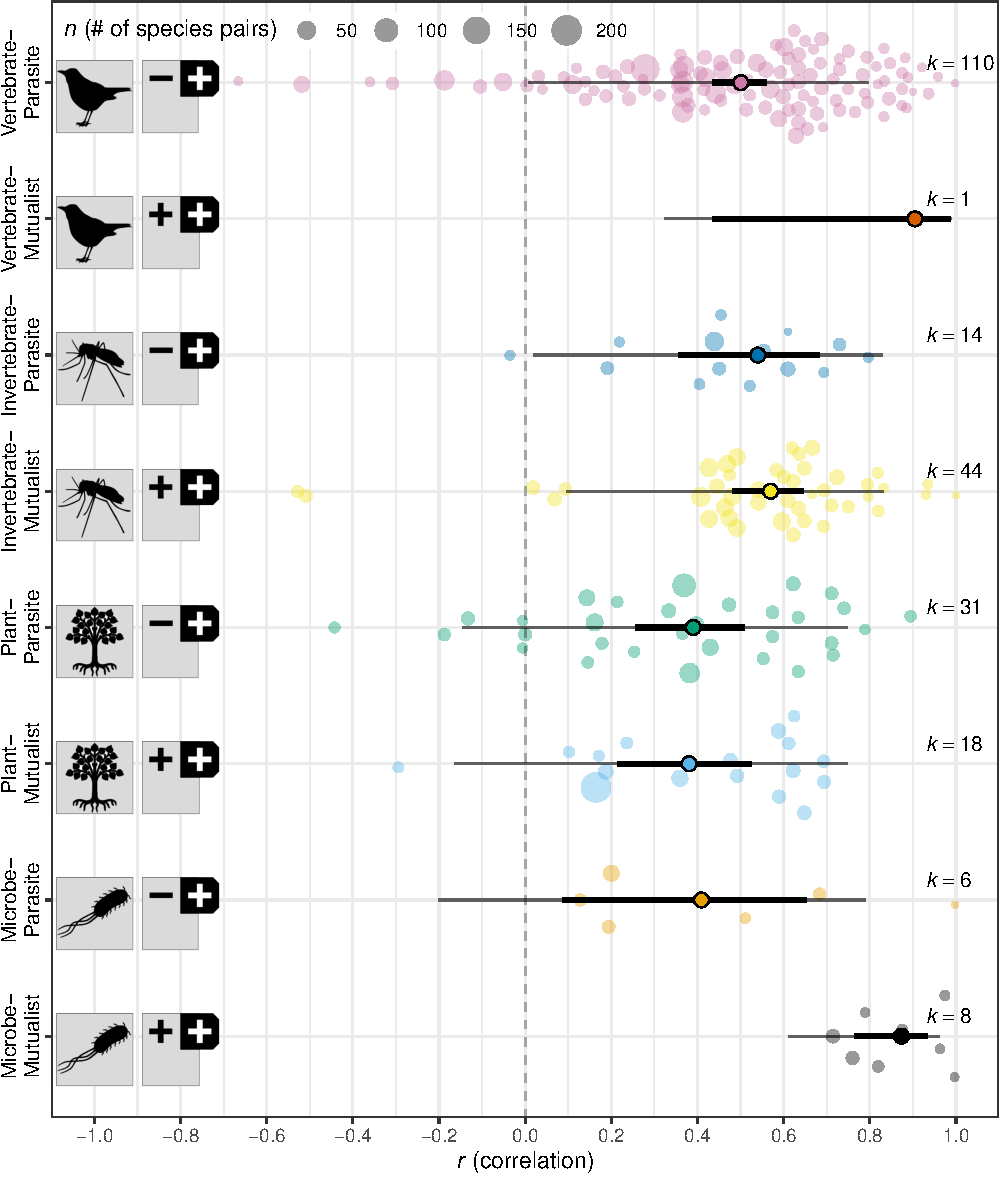
\includegraphics{Supporting_Information_files/figure-latex/unnamed-chunk-41-1.pdf}

\textbf{Supplementary Figure 3:} A forest plot showing group-wise means
(the categorical variable \texttt{host\_tax\_symbiosis}) with their 95\%
confidence intervals (thick lines) and 95\% prediction intervals (thin
lines), with observed effect sizes based on various sample sizes.

Splitting host taxonomy by mode of symbiosis revealed that the observed
higher phylogenetic congruence of host-symbiont cophylogenies involving
a microbial host is driven primarily by greater congruence between
microbial hosts and mutualist symbionts. Congruence is also relatively
high for invertebrate hosts that harbour a mutualistic symbiont, while
congruence appears to be lowest for plant hosts that harbour a parasitic
symbiont.

\hypertarget{the-combined-effect-of-symbiont-taxa-and-symbiosis-parasitism-vs.-mutualism}{%
\paragraph{The combined effect of symbiont taxa and symbiosis
(parasitism
vs.~mutualism)}\label{the-combined-effect-of-symbiont-taxa-and-symbiosis-parasitism-vs.-mutualism}}

\begin{Shaded}
\begin{Highlighting}[]
\CommentTok{# reordering}
\NormalTok{dat}\OperatorTok{$}\NormalTok{symbiont_tax_symbiosis <-}\StringTok{ }\KeywordTok{factor}\NormalTok{(dat}\OperatorTok{$}\NormalTok{symbiont_tax_symbiosis, }\DataTypeTok{levels =} \KeywordTok{c}\NormalTok{(}\StringTok{"MicrobeMutualist"}\NormalTok{, }
    \StringTok{"MicrobeParasite"}\NormalTok{, }\StringTok{"PlantMutualist"}\NormalTok{, }\StringTok{"PlantParasite"}\NormalTok{, }\StringTok{"InvertMutualist"}\NormalTok{, }\StringTok{"InvertParasite"}\NormalTok{, }
    \StringTok{"VertParasite"}\NormalTok{))}

\CommentTok{# meta-regression: multiple intercepts}
\NormalTok{mr_symbiont_tax_symbiosis1 <-}\StringTok{ }\KeywordTok{rma.mv}\NormalTok{(}\DataTypeTok{yi =}\NormalTok{ Zr, }\DataTypeTok{V =}\NormalTok{ VZr, }\DataTypeTok{mods =} \OperatorTok{~}\NormalTok{symbiont_tax_symbiosis }\OperatorTok{-}\StringTok{ }
\StringTok{    }\DecValTok{1}\NormalTok{, }\DataTypeTok{test =} \StringTok{"t"}\NormalTok{, }\DataTypeTok{random =} \OperatorTok{~}\DecValTok{1} \OperatorTok{|}\StringTok{ }\NormalTok{authors, }\DataTypeTok{data =}\NormalTok{ dat)}

\CommentTok{# # meta-regression: contrasts x 10 getting the level names out}
\NormalTok{level_names <-}\StringTok{ }\KeywordTok{levels}\NormalTok{(dat}\OperatorTok{$}\NormalTok{symbiont_tax_symbiosis)}

\CommentTok{# helper function to run metafor meta-regression}
\NormalTok{run_rma <-}\StringTok{ }\ControlFlowTok{function}\NormalTok{(name) \{}
    \KeywordTok{rma.mv}\NormalTok{(}\DataTypeTok{yi =}\NormalTok{ Zr, }\DataTypeTok{V =}\NormalTok{ VZr, }\DataTypeTok{mods =} \OperatorTok{~}\KeywordTok{relevel}\NormalTok{(symbiont_tax_symbiosis, }\DataTypeTok{ref =}\NormalTok{ name), }
        \DataTypeTok{test =} \StringTok{"t"}\NormalTok{, }\DataTypeTok{random =} \OperatorTok{~}\DecValTok{1} \OperatorTok{|}\StringTok{ }\NormalTok{authors, }\DataTypeTok{data =}\NormalTok{ dat)}
\NormalTok{\}}

\CommentTok{# results of meta-regression including all contrast results; taking the last}
\CommentTok{# level out ([-length(level_names)])}
\NormalTok{mr_symbiont_tax_symbiosis <-}\StringTok{ }\KeywordTok{map}\NormalTok{(level_names[}\OperatorTok{-}\KeywordTok{length}\NormalTok{(level_names)], run_rma)}
\end{Highlighting}
\end{Shaded}

\textbf{Supplementary Table 11:} Regression coefficients (Estimate),
95\% confidence intervals (CIs), variance components (V) and variance
explained, \emph{R}\textsuperscript{2}\textsubscript{{[}marginal{]}}
(R2) from the meta-regression with \texttt{symbiont\_tax\_symbiosis}.

\begin{Shaded}
\begin{Highlighting}[]
\CommentTok{# getting marginal R2}
\NormalTok{r2_symbiont_tax_symbiosis1 <-}\StringTok{ }\KeywordTok{R2}\NormalTok{(mr_symbiont_tax_symbiosis1)}

\CommentTok{# getting estimates}
\NormalTok{res_symbiont_tax_symbiosis1 <-}\StringTok{ }\KeywordTok{get_est}\NormalTok{(mr_symbiont_tax_symbiosis1, }\DataTypeTok{mod =} \StringTok{"symbiont_tax_symbiosis"}\NormalTok{)}
\NormalTok{res_symbiont_tax_symbiosis <-}\StringTok{ }\KeywordTok{map}\NormalTok{(mr_symbiont_tax_symbiosis, }\OperatorTok{~}\KeywordTok{get_est}\NormalTok{(.x, }\DataTypeTok{mod =} \StringTok{"symbiont_tax_symbiosis"}\NormalTok{))}

\CommentTok{# a list of the numbers to take out unnecessary contrasts}
\NormalTok{contra_list <-}\StringTok{ }\KeywordTok{Map}\NormalTok{(seq, }\DataTypeTok{from =} \DecValTok{1}\NormalTok{, }\DataTypeTok{to =} \DecValTok{1}\OperatorTok{:}\DecValTok{6}\NormalTok{)}

\CommentTok{# you need to flatten twice: first to make it a list and make it a vector}
\NormalTok{estimates <-}\StringTok{ }\KeywordTok{map2}\NormalTok{(res_symbiont_tax_symbiosis, contra_list, }\OperatorTok{~}\NormalTok{.x[}\OperatorTok{-}\NormalTok{(.y), }\StringTok{"estimate"}\NormalTok{]) }\OperatorTok\StringTok{ }
\StringTok{    }\KeywordTok{flatten}\NormalTok{() }\OperatorTok\StringTok{ }\KeywordTok{flatten_dbl}\NormalTok{()}
\NormalTok{lowerCLs <-}\StringTok{ }\KeywordTok{map2}\NormalTok{(res_symbiont_tax_symbiosis, contra_list, }\OperatorTok{~}\NormalTok{.x[}\OperatorTok{-}\NormalTok{(.y), }\StringTok{"lowerCL"}\NormalTok{]) }\OperatorTok\StringTok{ }
\StringTok{    }\KeywordTok{flatten}\NormalTok{() }\OperatorTok\StringTok{ }\KeywordTok{flatten_dbl}\NormalTok{()}
\NormalTok{upperCLs <-}\StringTok{ }\KeywordTok{map2}\NormalTok{(res_symbiont_tax_symbiosis, contra_list, }\OperatorTok{~}\NormalTok{.x[}\OperatorTok{-}\NormalTok{(.y), }\StringTok{"upperCL"}\NormalTok{]) }\OperatorTok\StringTok{ }
\StringTok{    }\KeywordTok{flatten}\NormalTok{() }\OperatorTok\StringTok{ }\KeywordTok{flatten_dbl}\NormalTok{()}

\CommentTok{# creating a table}
\KeywordTok{tibble}\NormalTok{(}\StringTok{`}\DataTypeTok{Fixed effect}\StringTok{`}\NormalTok{ =}\StringTok{ }\KeywordTok{c}\NormalTok{(}\KeywordTok{as.character}\NormalTok{(res_symbiont_tax_symbiosis1}\OperatorTok{$}\NormalTok{name), }\KeywordTok{cont_gen}\NormalTok{(res_symbiont_tax_symbiosis1}\OperatorTok{$}\NormalTok{name)), }
    \DataTypeTok{Estimate =} \KeywordTok{c}\NormalTok{(res_symbiont_tax_symbiosis1}\OperatorTok{$}\NormalTok{estimate, estimates), }\StringTok{`}\DataTypeTok{Lower CI [0.025]}\StringTok{`}\NormalTok{ =}\StringTok{ }\KeywordTok{c}\NormalTok{(res_symbiont_tax_symbiosis1}\OperatorTok{$}\NormalTok{lowerCL, }
\NormalTok{        lowerCLs), }\StringTok{`}\DataTypeTok{Upper CI  [0.975]}\StringTok{`}\NormalTok{ =}\StringTok{ }\KeywordTok{c}\NormalTok{(res_symbiont_tax_symbiosis1}\OperatorTok{$}\NormalTok{upperCL, upperCLs), }
    \StringTok{`}\DataTypeTok{V[authors]}\StringTok{`}\NormalTok{ =}\StringTok{ }\KeywordTok{c}\NormalTok{(mr_symbiont_tax_symbiosis1}\OperatorTok{$}\NormalTok{sigma2, }\KeywordTok{rep}\NormalTok{(}\OtherTok{NA}\NormalTok{, (}\DecValTok{7} \OperatorTok{+}\StringTok{ }\KeywordTok{choose}\NormalTok{(}\DecValTok{7}\NormalTok{, }\DecValTok{2}\NormalTok{)) }\OperatorTok{-}\StringTok{ }
\StringTok{        }\DecValTok{1}\NormalTok{)), }\DataTypeTok{R2 =} \KeywordTok{c}\NormalTok{(r2_symbiont_tax_symbiosis1[}\DecValTok{1}\NormalTok{], }\KeywordTok{rep}\NormalTok{(}\OtherTok{NA}\NormalTok{, (}\DecValTok{7} \OperatorTok{+}\StringTok{ }\KeywordTok{choose}\NormalTok{(}\DecValTok{7}\NormalTok{, }\DecValTok{2}\NormalTok{)) }\OperatorTok{-}\StringTok{ }\DecValTok{1}\NormalTok{))) }\OperatorTok\StringTok{ }
\StringTok{    }\KeywordTok{kable}\NormalTok{(}\StringTok{"html"}\NormalTok{, }\DataTypeTok{digits =} \DecValTok{3}\NormalTok{) }\OperatorTok\StringTok{ }\KeywordTok{kable_styling}\NormalTok{(}\StringTok{"striped"}\NormalTok{, }\DataTypeTok{position =} \StringTok{"left"}\NormalTok{) }\OperatorTok\StringTok{ }
\StringTok{    }\KeywordTok{scroll_box}\NormalTok{(}\DataTypeTok{width =} \StringTok{"100%"}\NormalTok{, }\DataTypeTok{height =} \StringTok{"300px"}\NormalTok{)}
\end{Highlighting}
\end{Shaded}

Fixed effect

Estimate

Lower CI {[}0.025{]}

Upper CI {[}0.975{]}

V{[}authors{]}

R2

MicrobeMutualist

0.687

0.570

0.804

0.082

0.357

MicrobeParasite

0.472

0.361

0.583

NA

NA

PlantMutualist

1.052

0.560

1.545

NA

NA

PlantParasite

3.453

1.404

5.503

NA

NA

InvertMutualist

0.474

0.269

0.680

NA

NA

InvertParasite

0.555

0.461

0.648

NA

NA

VertParasite

0.496

-0.157

1.149

NA

NA

MicrobeMutualist-MicrobeParasite

-0.215

-0.376

-0.054

NA

NA

MicrobeMutualist-PlantMutualist

0.366

-0.140

0.872

NA

NA

MicrobeMutualist-PlantParasite

2.766

0.713

4.820

NA

NA

MicrobeMutualist-InvertMutualist

-0.212

-0.449

0.024

NA

NA

MicrobeMutualist-InvertParasite

-0.132

-0.282

0.018

NA

NA

MicrobeMutualist-VertParasite

-0.191

-0.855

0.472

NA

NA

MicrobeParasite-PlantMutualist

0.580

0.076

1.085

NA

NA

MicrobeParasite-PlantParasite

2.981

0.928

5.034

NA

NA

MicrobeParasite-InvertMutualist

0.002

-0.231

0.236

NA

NA

MicrobeParasite-InvertParasite

0.082

-0.063

0.228

NA

NA

MicrobeParasite-VertParasite

0.023

-0.639

0.686

NA

NA

PlantMutualist-PlantParasite

2.401

0.293

4.509

NA

NA

PlantMutualist-InvertMutualist

-0.578

-1.111

-0.045

NA

NA

PlantMutualist-InvertParasite

-0.498

-0.999

0.003

NA

NA

PlantMutualist-VertParasite

-0.557

-1.375

0.261

NA

NA

PlantParasite-InvertMutualist

-2.979

-5.039

-0.919

NA

NA

PlantParasite-InvertParasite

-2.899

-4.951

-0.847

NA

NA

PlantParasite-VertParasite

-2.958

-5.109

-0.806

NA

NA

InvertMutualist-InvertParasite

0.080

-0.138

0.298

NA

NA

InvertMutualist-VertParasite

0.021

-0.663

0.706

NA

NA

InvertParasite-VertParasite

-0.059

-0.719

0.601

NA

NA

\begin{Shaded}
\begin{Highlighting}[]
\CommentTok{# adding sample size (k) for each category}
\NormalTok{k_symbiont_tax_symbiosis <-}\StringTok{ }\NormalTok{dat }\OperatorTok\StringTok{ }\KeywordTok{group_by}\NormalTok{(symbiont_tax_symbiosis) }\OperatorTok\StringTok{ }\KeywordTok{count}\NormalTok{()}
\CommentTok{# getting estimates and predicitons}
\NormalTok{pred_symbiont_tax_symbiosis <-}\StringTok{ }\KeywordTok{get_pred}\NormalTok{(mr_symbiont_tax_symbiosis1, }\DataTypeTok{mod =} \StringTok{"symbiont_tax_symbiosis"}\NormalTok{) }
\NormalTok{res_symbiont_tax_symbiosis1 <-}\StringTok{ }\KeywordTok{left_join}\NormalTok{(res_symbiont_tax_symbiosis1, k_symbiont_tax_symbiosis, }\DataTypeTok{by =}  \KeywordTok{c}\NormalTok{(}\StringTok{"name"}\NormalTok{ =}\StringTok{ "symbiont_tax_symbiosis"}\NormalTok{))  }\OperatorTok\StringTok{ }\KeywordTok{left_join}\NormalTok{(pred_symbiont_tax_symbiosis)}
\CommentTok{#res_symbiosis1 }
\CommentTok{# drawing a funnel plot - fig 2b}
\NormalTok{fig_symbiont_tax_symbiosis <-}\StringTok{ }\KeywordTok{ggplot}\NormalTok{(}\DataTypeTok{data =}\NormalTok{ res_symbiont_tax_symbiosis1, }\KeywordTok{aes}\NormalTok{(}\DataTypeTok{x =} \KeywordTok{tanh}\NormalTok{(estimate), }\DataTypeTok{y =}\NormalTok{ name)) }\OperatorTok{+}
\StringTok{  }\KeywordTok{scale_x_continuous}\NormalTok{(}\DataTypeTok{limits=}\KeywordTok{c}\NormalTok{(}\OperatorTok{-}\DecValTok{1}\NormalTok{, }\DecValTok{1}\NormalTok{), }\DataTypeTok{breaks =} \KeywordTok{seq}\NormalTok{(}\OperatorTok{-}\DecValTok{1}\NormalTok{, }\DecValTok{1}\NormalTok{, }\DataTypeTok{by =} \FloatTok{0.2}\NormalTok{) ) }\OperatorTok{+}
\StringTok{  }\KeywordTok{geom_quasirandom}\NormalTok{(}\DataTypeTok{data =}\NormalTok{ dat }\OperatorTok\StringTok{ }\KeywordTok{filter}\NormalTok{(}\OperatorTok{!}\KeywordTok{is.na}\NormalTok{(symbiont_tax_symbiosis)), }
                   \KeywordTok{aes}\NormalTok{(}\DataTypeTok{x=} \KeywordTok{tanh}\NormalTok{(Zr), }\DataTypeTok{y =}\NormalTok{ symbiont_tax_symbiosis, }\DataTypeTok{size =}\NormalTok{ ((}\DecValTok{1}\OperatorTok{/}\NormalTok{VZr) }\OperatorTok{+}\StringTok{ }\DecValTok{3}\NormalTok{), }\DataTypeTok{colour =}\NormalTok{ symbiont_tax_symbiosis), }\DataTypeTok{groupOnX =} \OtherTok{FALSE}\NormalTok{, }\DataTypeTok{alpha=}\FloatTok{0.4}\NormalTok{) }\OperatorTok{+}\StringTok{ }
\StringTok{  }\CommentTok{# 95 %precition interval (PI)}
\StringTok{  }\KeywordTok{geom_errorbarh}\NormalTok{(}\KeywordTok{aes}\NormalTok{(}\DataTypeTok{xmin =} \KeywordTok{tanh}\NormalTok{(lowerPR), }\DataTypeTok{xmax =} \KeywordTok{tanh}\NormalTok{(upperPR)),  }\DataTypeTok{height =} \DecValTok{0}\NormalTok{, }\DataTypeTok{show.legend =}\NormalTok{ F, }\DataTypeTok{size =} \FloatTok{0.5}\NormalTok{, }\DataTypeTok{alpha =} \FloatTok{0.6}\NormalTok{) }\OperatorTok{+}
\StringTok{  }\CommentTok{# 95 %CI}
\StringTok{  }\KeywordTok{geom_errorbarh}\NormalTok{(}\KeywordTok{aes}\NormalTok{(}\DataTypeTok{xmin =} \KeywordTok{tanh}\NormalTok{(lowerCL), }\DataTypeTok{xmax =} \KeywordTok{tanh}\NormalTok{(upperCL)),  }\DataTypeTok{height =} \DecValTok{0}\NormalTok{, }\DataTypeTok{show.legend =}\NormalTok{ F, }\DataTypeTok{size =} \FloatTok{1.2}\NormalTok{) }\OperatorTok{+}
\StringTok{  }\KeywordTok{geom_vline}\NormalTok{(}\DataTypeTok{xintercept =} \DecValTok{0}\NormalTok{, }\DataTypeTok{linetype =} \DecValTok{2}\NormalTok{, }\DataTypeTok{colour =} \StringTok{"black"}\NormalTok{, }\DataTypeTok{alpha =} \FloatTok{0.3}\NormalTok{) }\OperatorTok{+}
\StringTok{  }\CommentTok{# creating dots and different size (bee-swarm and bubbles)}
\StringTok{  }\KeywordTok{geom_point}\NormalTok{(}\KeywordTok{aes}\NormalTok{(}\DataTypeTok{fill =}\NormalTok{ name), }\DataTypeTok{size =} \DecValTok{3}\NormalTok{, }\DataTypeTok{shape =} \DecValTok{21}\NormalTok{) }\OperatorTok{+}\StringTok{ }\CommentTok{#}
\StringTok{  }\CommentTok{# setting colours}
\StringTok{  }\CommentTok{# setting colours}
\StringTok{  }\KeywordTok{scale_color_manual}\NormalTok{(}\DataTypeTok{values =}   \KeywordTok{c}\NormalTok{(}\StringTok{"MicrobeMutualist"}\NormalTok{=}\StringTok{ }\NormalTok{colour_ls[}\DecValTok{1}\NormalTok{], }\StringTok{"MicrobeParasite"}\NormalTok{=}\StringTok{ }\NormalTok{colour_ls[}\DecValTok{2}\NormalTok{],  }\StringTok{"PlantMutualist"}\NormalTok{=}\StringTok{ }\NormalTok{colour_ls[}\DecValTok{3}\NormalTok{], }\StringTok{"PlantParasite"}\NormalTok{=}\StringTok{ }\NormalTok{colour_ls[}\DecValTok{4}\NormalTok{], }\StringTok{"InvertMutualist"}\NormalTok{ =}\StringTok{ }\NormalTok{colour_ls[}\DecValTok{5}\NormalTok{],  }\StringTok{"InvertParasite"}\NormalTok{=}\StringTok{ }\NormalTok{colour_ls[}\DecValTok{6}\NormalTok{], }\StringTok{"VertParasite"}\NormalTok{=}\StringTok{ }\NormalTok{colour_ls[}\DecValTok{8}\NormalTok{] )) }\OperatorTok{+}
\StringTok{  }\KeywordTok{scale_fill_manual}\NormalTok{(}\DataTypeTok{values =} \KeywordTok{c}\NormalTok{(}\StringTok{"MicrobeMutualist"}\NormalTok{=}\StringTok{ }\NormalTok{colour_ls[}\DecValTok{1}\NormalTok{], }\StringTok{"MicrobeParasite"}\NormalTok{=}\StringTok{ }\NormalTok{colour_ls[}\DecValTok{2}\NormalTok{],  }\StringTok{"PlantMutualist"}\NormalTok{=}\StringTok{ }\NormalTok{colour_ls[}\DecValTok{3}\NormalTok{], }\StringTok{"PlantParasite"}\NormalTok{=}\StringTok{ }\NormalTok{colour_ls[}\DecValTok{4}\NormalTok{], }\StringTok{"InvertMutualist"}\NormalTok{ =}\StringTok{ }\NormalTok{colour_ls[}\DecValTok{5}\NormalTok{],  }\StringTok{"InvertParasite"}\NormalTok{=}\StringTok{ }\NormalTok{colour_ls[}\DecValTok{6}\NormalTok{], }\StringTok{"VertParasite"}\NormalTok{=}\StringTok{ }\NormalTok{colour_ls[}\DecValTok{8}\NormalTok{] )) }\OperatorTok{+}
\StringTok{  }\KeywordTok{scale_y_discrete}\NormalTok{(}\DataTypeTok{labels =} \KeywordTok{c}\NormalTok{(}\StringTok{"MicrobeMutualist"}\NormalTok{=}\StringTok{ "Microbe-}\CharTok{\textbackslash{}n}\StringTok{Mutualist"}\NormalTok{, }\StringTok{"MicrobeParasite"}\NormalTok{=}\StringTok{ "Microbe-}\CharTok{\textbackslash{}n}\StringTok{Parasite"}\NormalTok{,  }\StringTok{"PlantMutualist"}\NormalTok{ =}\StringTok{ "Plant-}\CharTok{\textbackslash{}n}\StringTok{Mutualist"}\NormalTok{, }\StringTok{"PlantParasite"}\NormalTok{=}\StringTok{"Plant-}\CharTok{\textbackslash{}n}\StringTok{Parasite"}\NormalTok{, }\StringTok{"InvertMutualist"}\NormalTok{ =}\StringTok{ "Invertebrate-}\CharTok{\textbackslash{}n}\StringTok{Mutualist"}\NormalTok{,   }\StringTok{"InvertParasite"}\NormalTok{=}\StringTok{ "Invertebrate-}\CharTok{\textbackslash{}n}\StringTok{Parasite"}\NormalTok{,  }\StringTok{"VertParasite"}\NormalTok{=}\StringTok{ "Vertebrate-}\CharTok{\textbackslash{}n}\StringTok{Parasite"}\NormalTok{ )) }\OperatorTok{+}
\StringTok{  }\KeywordTok{annotate}\NormalTok{(}\StringTok{'text'}\NormalTok{, }\DataTypeTok{x =} \FloatTok{0.93}\NormalTok{, }\DataTypeTok{y =} \DecValTok{1}\OperatorTok{:}\DecValTok{7} \OperatorTok{+}\StringTok{ }\FloatTok{0.15}\NormalTok{, }\DataTypeTok{label=} \KeywordTok{paste}\NormalTok{(}\StringTok{"italic(k)=="}\NormalTok{, res_symbiont_tax_symbiosis1}\OperatorTok{$}\NormalTok{n), }\DataTypeTok{parse=}\OtherTok{TRUE}\NormalTok{, }\DataTypeTok{hjust =} \StringTok{"left"}\NormalTok{, }\DataTypeTok{size=}\FloatTok{3.5}\NormalTok{) }\OperatorTok{+}
\StringTok{  }\KeywordTok{labs}\NormalTok{(}\DataTypeTok{x =} \KeywordTok{expression}\NormalTok{(}\KeywordTok{paste}\NormalTok{(}\KeywordTok{italic}\NormalTok{(r), }\StringTok{" (correlation)"}\NormalTok{)), }\DataTypeTok{y =} \StringTok{""}\NormalTok{, }\DataTypeTok{size =} \KeywordTok{expression}\NormalTok{(}\KeywordTok{paste}\NormalTok{(}\KeywordTok{italic}\NormalTok{(n), }\StringTok{" (# of species pairs)"}\NormalTok{)) ) }\OperatorTok{+}
\StringTok{  }\KeywordTok{guides}\NormalTok{(}\DataTypeTok{fill =} \StringTok{"none"}\NormalTok{, }\DataTypeTok{colour =} \StringTok{"none"}\NormalTok{) }\OperatorTok{+}
\StringTok{  }\KeywordTok{theme_bw}\NormalTok{() }\OperatorTok{+}
\StringTok{  }\KeywordTok{theme}\NormalTok{(}\DataTypeTok{legend.position=} \KeywordTok{c}\NormalTok{(}\DecValTok{0}\NormalTok{, }\DecValTok{1}\NormalTok{), }\DataTypeTok{legend.justification =} \KeywordTok{c}\NormalTok{(}\DecValTok{0}\NormalTok{, }\DecValTok{1}\NormalTok{)) }\OperatorTok{+}
\StringTok{  }\KeywordTok{theme}\NormalTok{(}\DataTypeTok{legend.direction=}\StringTok{"horizontal"}\NormalTok{) }\OperatorTok{+}
\StringTok{  }\CommentTok{#theme(legend.background = element_rect(fill = "white", colour = "black")) +}
\StringTok{  }\KeywordTok{theme}\NormalTok{(}\DataTypeTok{legend.background =} \KeywordTok{element_blank}\NormalTok{()) }\OperatorTok{+}
\StringTok{  }\KeywordTok{theme}\NormalTok{(}\DataTypeTok{axis.text.y =} \KeywordTok{element_text}\NormalTok{(}\DataTypeTok{size =} \DecValTok{10}\NormalTok{, }\DataTypeTok{colour =}\StringTok{"black"}\NormalTok{, }\DataTypeTok{hjust =} \FloatTok{0.5}\NormalTok{, }\DataTypeTok{angle =} \DecValTok{90}\NormalTok{)) }\OperatorTok{+}
\StringTok{    }\CommentTok{# putting pictures in}
\StringTok{  }\KeywordTok{annotation_custom}\NormalTok{(}\KeywordTok{rasterGrob}\NormalTok{(image_microbe_parasite), }\DataTypeTok{xmin =} \FloatTok{-1.1}\NormalTok{, }\DataTypeTok{xmax =} \FloatTok{-0.9}\NormalTok{, }\DataTypeTok{ymin =} \FloatTok{0.6}\NormalTok{, }\DataTypeTok{ymax =} \FloatTok{1.2}\NormalTok{) }\OperatorTok{+}\StringTok{ }
\StringTok{  }\KeywordTok{annotation_custom}\NormalTok{(}\KeywordTok{rasterGrob}\NormalTok{(image_mutualism), }\DataTypeTok{xmin =} \FloatTok{-0.9}\NormalTok{, }\DataTypeTok{xmax =} \FloatTok{-0.7}\NormalTok{, }\DataTypeTok{ymin =} \FloatTok{0.6}\NormalTok{, }\DataTypeTok{ymax =} \FloatTok{1.2}\NormalTok{) }\OperatorTok{+}\StringTok{ }
\StringTok{  }\KeywordTok{annotation_custom}\NormalTok{(}\KeywordTok{rasterGrob}\NormalTok{(image_microbe_parasite), }\DataTypeTok{xmin =} \FloatTok{-1.1}\NormalTok{, }\DataTypeTok{xmax =} \FloatTok{-0.9}\NormalTok{, }\DataTypeTok{ymin =} \FloatTok{1.6}\NormalTok{, }\DataTypeTok{ymax =} \FloatTok{2.2}\NormalTok{) }\OperatorTok{+}
\StringTok{  }\KeywordTok{annotation_custom}\NormalTok{(}\KeywordTok{rasterGrob}\NormalTok{(image_parasitism),}\DataTypeTok{xmin =} \FloatTok{-0.9}\NormalTok{, }\DataTypeTok{xmax =} \FloatTok{-0.7}\NormalTok{, }\DataTypeTok{ymin =} \FloatTok{1.6}\NormalTok{, }\DataTypeTok{ymax =} \FloatTok{2.2}\NormalTok{) }\OperatorTok{+}
\StringTok{  }\KeywordTok{annotation_custom}\NormalTok{(}\KeywordTok{rasterGrob}\NormalTok{(image_plant_parasite), }\DataTypeTok{xmin =} \FloatTok{-1.1}\NormalTok{, }\DataTypeTok{xmax =} \FloatTok{-0.9}\NormalTok{, }\DataTypeTok{ymin =} \FloatTok{2.6}\NormalTok{, }\DataTypeTok{ymax =} \FloatTok{3.2}\NormalTok{) }\OperatorTok{+}\StringTok{ }
\StringTok{  }\KeywordTok{annotation_custom}\NormalTok{(}\KeywordTok{rasterGrob}\NormalTok{(image_mutualism), }\DataTypeTok{xmin =} \FloatTok{-0.9}\NormalTok{, }\DataTypeTok{xmax =} \FloatTok{-0.7}\NormalTok{, }\DataTypeTok{ymin =} \FloatTok{2.6}\NormalTok{, }\DataTypeTok{ymax =} \FloatTok{3.2}\NormalTok{) }\OperatorTok{+}\StringTok{ }
\StringTok{  }\KeywordTok{annotation_custom}\NormalTok{(}\KeywordTok{rasterGrob}\NormalTok{(image_plant_parasite), }\DataTypeTok{xmin =} \FloatTok{-1.1}\NormalTok{, }\DataTypeTok{xmax =} \FloatTok{-0.9}\NormalTok{, }\DataTypeTok{ymin =} \FloatTok{3.6}\NormalTok{, }\DataTypeTok{ymax =} \FloatTok{4.2}\NormalTok{) }\OperatorTok{+}
\StringTok{  }\KeywordTok{annotation_custom}\NormalTok{(}\KeywordTok{rasterGrob}\NormalTok{(image_parasitism), }\DataTypeTok{xmin =} \FloatTok{-0.9}\NormalTok{, }\DataTypeTok{xmax =} \FloatTok{-0.7}\NormalTok{, }\DataTypeTok{ymin =} \FloatTok{3.6}\NormalTok{, }\DataTypeTok{ymax =} \FloatTok{4.2}\NormalTok{) }\OperatorTok{+}
\StringTok{  }\KeywordTok{annotation_custom}\NormalTok{(}\KeywordTok{rasterGrob}\NormalTok{(image_invertebrate_parasite), }\DataTypeTok{xmin =} \FloatTok{-1.1}\NormalTok{, }\DataTypeTok{xmax =} \FloatTok{-0.9}\NormalTok{, }\DataTypeTok{ymin =} \FloatTok{4.6}\NormalTok{, }\DataTypeTok{ymax =} \FloatTok{5.2}\NormalTok{) }\OperatorTok{+}
\StringTok{  }\KeywordTok{annotation_custom}\NormalTok{(}\KeywordTok{rasterGrob}\NormalTok{(image_mutualism), }\DataTypeTok{xmin =} \FloatTok{-0.9}\NormalTok{, }\DataTypeTok{xmax =} \FloatTok{-0.7}\NormalTok{, }\DataTypeTok{ymin =} \FloatTok{4.6}\NormalTok{, }\DataTypeTok{ymax =} \FloatTok{5.2}\NormalTok{) }\OperatorTok{+}
\StringTok{  }\KeywordTok{annotation_custom}\NormalTok{(}\KeywordTok{rasterGrob}\NormalTok{(image_invertebrate_parasite), }\DataTypeTok{xmin =} \FloatTok{-1.1}\NormalTok{, }\DataTypeTok{xmax =} \FloatTok{-0.9}\NormalTok{, }\DataTypeTok{ymin =} \FloatTok{5.6}\NormalTok{, }\DataTypeTok{ymax =} \FloatTok{6.2}\NormalTok{) }\OperatorTok{+}\StringTok{ }
\StringTok{  }\KeywordTok{annotation_custom}\NormalTok{(}\KeywordTok{rasterGrob}\NormalTok{(image_parasitism), }\DataTypeTok{xmin =} \FloatTok{-0.9}\NormalTok{, }\DataTypeTok{xmax =} \FloatTok{-0.7}\NormalTok{, }\DataTypeTok{ymin =} \FloatTok{5.6}\NormalTok{, }\DataTypeTok{ymax =} \FloatTok{6.2}\NormalTok{) }\OperatorTok{+}\StringTok{ }
\StringTok{  }\KeywordTok{annotation_custom}\NormalTok{(}\KeywordTok{rasterGrob}\NormalTok{(image_vertebrate_parasite), }\DataTypeTok{xmin =} \FloatTok{-1.1}\NormalTok{, }\DataTypeTok{xmax =} \FloatTok{-0.9}\NormalTok{, }\DataTypeTok{ymin =} \FloatTok{6.6}\NormalTok{, }\DataTypeTok{ymax =} \FloatTok{7.2}\NormalTok{) }\OperatorTok{+}
\StringTok{  }\KeywordTok{annotation_custom}\NormalTok{(}\KeywordTok{rasterGrob}\NormalTok{(image_parasitism), }\DataTypeTok{xmin =} \FloatTok{-0.9}\NormalTok{, }\DataTypeTok{xmax =} \FloatTok{-0.7}\NormalTok{, }\DataTypeTok{ymin =} \FloatTok{6.6}\NormalTok{, }\DataTypeTok{ymax =} \FloatTok{7.2}\NormalTok{) }

\NormalTok{fig_symbiont_tax_symbiosis}
\end{Highlighting}
\end{Shaded}

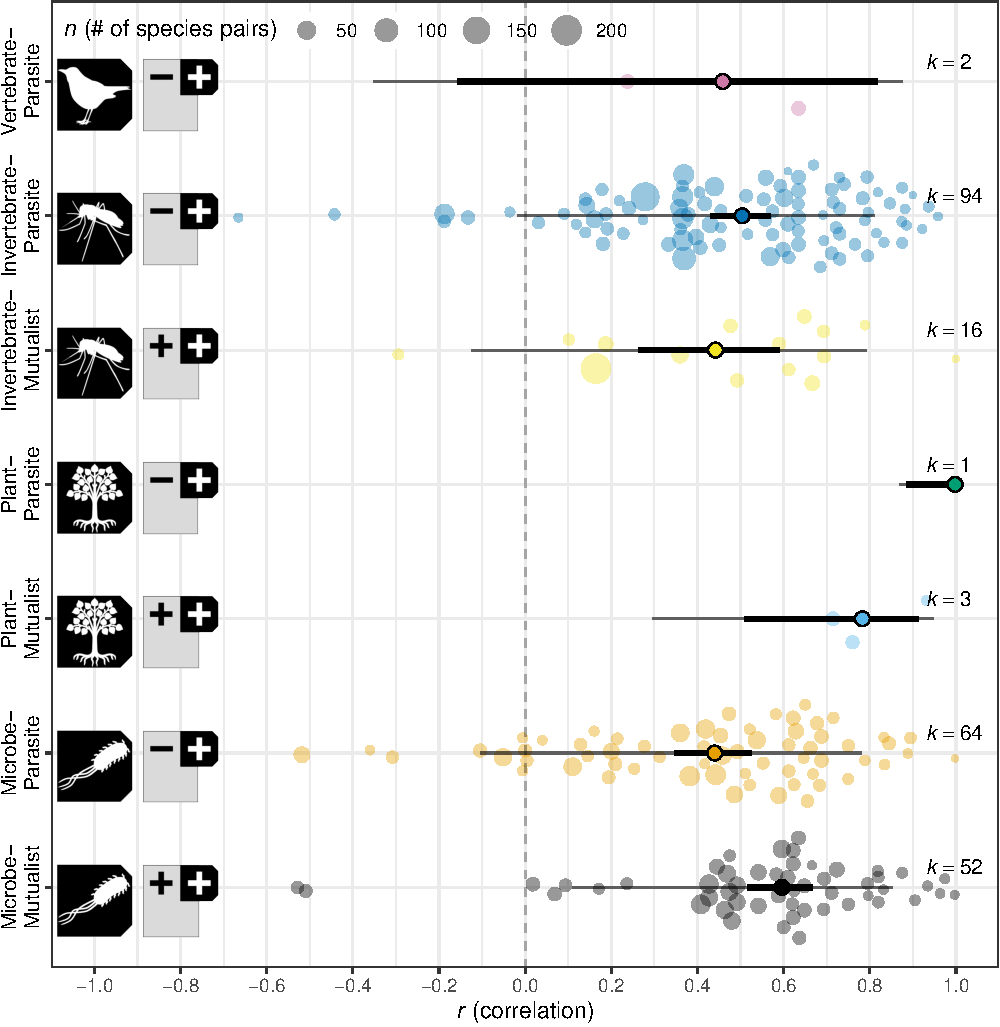
\includegraphics{Supporting_Information_files/figure-latex/unnamed-chunk-44-1.pdf}

\textbf{Supplementary Figure 4:} A forest plot showing group-wise means
(the categorical variable \texttt{symbiont\_tax\_symbiosis}) with their
95\% confidence intervals (thick lines) and 95\% prediction intervals
(thin lines), with observed effect sizes based on various sample sizes.

Splitting symbiont taxonomy by mode of symbiosis revealed much less
variation, except for higher congruence exhibited by cophylogenies
involving a plant symbiont (instances of which are relatively rare), and
the finding that cophylogenies involving a microbial mutualist symbiont
are slightly more congruent than the remaining categories.

\hypertarget{the-combined-effect-of-host-and-symbiont-taxa}{%
\paragraph{The combined effect of host and symbiont
taxa}\label{the-combined-effect-of-host-and-symbiont-taxa}}

\begin{Shaded}
\begin{Highlighting}[]
\CommentTok{# reordering}
\NormalTok{dat}\OperatorTok{$}\NormalTok{host_symbiont_tax <-}\StringTok{ }\KeywordTok{factor}\NormalTok{(dat}\OperatorTok{$}\NormalTok{host_symbiont_tax, }\DataTypeTok{levels =} \KeywordTok{c}\NormalTok{(}\StringTok{"MicrobeInvert"}\NormalTok{, }
    \StringTok{"MicrobeMicrobe"}\NormalTok{, }\StringTok{"MicrobePlant"}\NormalTok{, }\StringTok{"PlantInvert"}\NormalTok{, }\StringTok{"PlantMicrobe"}\NormalTok{, }\StringTok{"InvertInvert"}\NormalTok{, }
    \StringTok{"InvertMicrobe"}\NormalTok{, }\StringTok{"InvertPlant"}\NormalTok{, }\StringTok{"VertInvert"}\NormalTok{, }\StringTok{"VertMicrobe"}\NormalTok{, }\StringTok{"VertVert"}\NormalTok{))}

\CommentTok{# meta-regression: multiple intercepts}
\NormalTok{mr_host_symbiont_tax1 <-}\StringTok{ }\KeywordTok{rma.mv}\NormalTok{(}\DataTypeTok{yi =}\NormalTok{ Zr, }\DataTypeTok{V =}\NormalTok{ VZr, }\DataTypeTok{mods =} \OperatorTok{~}\NormalTok{host_symbiont_tax }\OperatorTok{-}\StringTok{ }\DecValTok{1}\NormalTok{, }
    \DataTypeTok{test =} \StringTok{"t"}\NormalTok{, }\DataTypeTok{random =} \OperatorTok{~}\DecValTok{1} \OperatorTok{|}\StringTok{ }\NormalTok{authors, }\DataTypeTok{data =}\NormalTok{ dat)}

\CommentTok{# # meta-regression: contrasts x 10 getting the level names out}
\NormalTok{level_names <-}\StringTok{ }\KeywordTok{levels}\NormalTok{(dat}\OperatorTok{$}\NormalTok{host_symbiont_tax)}

\CommentTok{# helper function to run metafor meta-regression}
\NormalTok{run_rma <-}\StringTok{ }\ControlFlowTok{function}\NormalTok{(name) \{}
    \KeywordTok{rma.mv}\NormalTok{(}\DataTypeTok{yi =}\NormalTok{ Zr, }\DataTypeTok{V =}\NormalTok{ VZr, }\DataTypeTok{mods =} \OperatorTok{~}\KeywordTok{relevel}\NormalTok{(host_symbiont_tax, }\DataTypeTok{ref =}\NormalTok{ name), }\DataTypeTok{test =} \StringTok{"t"}\NormalTok{, }
        \DataTypeTok{random =} \OperatorTok{~}\DecValTok{1} \OperatorTok{|}\StringTok{ }\NormalTok{authors, }\DataTypeTok{data =}\NormalTok{ dat)}
\NormalTok{\}}

\CommentTok{# results of meta-regression including all contrast results; taking the last}
\CommentTok{# level out ([-length(level_names)])}
\NormalTok{mr_host_symbiont_tax <-}\StringTok{ }\KeywordTok{map}\NormalTok{(level_names[}\OperatorTok{-}\KeywordTok{length}\NormalTok{(level_names)], run_rma)}
\end{Highlighting}
\end{Shaded}

\textbf{Supplementary Table 12:} Regression coefficients (estimate),
95\% confidence intervals (CIs), variance components (V) and variance
explained, \emph{R}\textsuperscript{2}\textsubscript{{[}marginal{]}}
(R2) from the meta-regression with \texttt{host\_symbiont\_tax}.

\begin{Shaded}
\begin{Highlighting}[]
\CommentTok{# getting marginal R2}
\NormalTok{r2_host_symbiont_tax1 <-}\StringTok{ }\KeywordTok{R2}\NormalTok{(mr_host_symbiont_tax1)}

\CommentTok{# getting estimates}
\NormalTok{res_host_symbiont_tax1 <-}\StringTok{ }\KeywordTok{get_est}\NormalTok{(mr_host_symbiont_tax1, }\DataTypeTok{mod =} \StringTok{"host_symbiont_tax"}\NormalTok{)}
\NormalTok{res_host_symbiont_tax <-}\StringTok{ }\KeywordTok{map}\NormalTok{(mr_host_symbiont_tax, }\OperatorTok{~}\KeywordTok{get_est}\NormalTok{(.x, }\DataTypeTok{mod =} \StringTok{"host_symbiont_tax"}\NormalTok{))}

\CommentTok{# a list of the numbers to take out unnecessary contrasts}
\NormalTok{contra_list <-}\StringTok{ }\KeywordTok{Map}\NormalTok{(seq, }\DataTypeTok{from =} \DecValTok{1}\NormalTok{, }\DataTypeTok{to =} \DecValTok{1}\OperatorTok{:}\DecValTok{10}\NormalTok{)}

\CommentTok{# you need to flatten twice: first to make it a list and make it a vector}
\NormalTok{estimates <-}\StringTok{ }\KeywordTok{map2}\NormalTok{(res_host_symbiont_tax, contra_list, }\OperatorTok{~}\NormalTok{.x[}\OperatorTok{-}\NormalTok{(.y), }\StringTok{"estimate"}\NormalTok{]) }\OperatorTok\StringTok{ }
\StringTok{    }\KeywordTok{flatten}\NormalTok{() }\OperatorTok\StringTok{ }\KeywordTok{flatten_dbl}\NormalTok{()}

\NormalTok{lowerCLs <-}\StringTok{ }\KeywordTok{map2}\NormalTok{(res_host_symbiont_tax, contra_list, }\OperatorTok{~}\NormalTok{.x[}\OperatorTok{-}\NormalTok{(.y), }\StringTok{"lowerCL"}\NormalTok{]) }\OperatorTok\StringTok{ }\KeywordTok{flatten}\NormalTok{() }\OperatorTok\StringTok{ }
\StringTok{    }\KeywordTok{flatten_dbl}\NormalTok{()}

\NormalTok{upperCLs <-}\StringTok{ }\KeywordTok{map2}\NormalTok{(res_host_symbiont_tax, contra_list, }\OperatorTok{~}\NormalTok{.x[}\OperatorTok{-}\NormalTok{(.y), }\StringTok{"upperCL"}\NormalTok{]) }\OperatorTok\StringTok{ }\KeywordTok{flatten}\NormalTok{() }\OperatorTok\StringTok{ }
\StringTok{    }\KeywordTok{flatten_dbl}\NormalTok{()}

\CommentTok{# creating a table}
\KeywordTok{tibble}\NormalTok{(}\StringTok{`}\DataTypeTok{Fixed effect}\StringTok{`}\NormalTok{ =}\StringTok{ }\KeywordTok{c}\NormalTok{(}\KeywordTok{as.character}\NormalTok{(res_host_symbiont_tax1}\OperatorTok{$}\NormalTok{name), }\KeywordTok{cont_gen}\NormalTok{(res_host_symbiont_tax1}\OperatorTok{$}\NormalTok{name)), }
    \DataTypeTok{Estimate =} \KeywordTok{c}\NormalTok{(res_host_symbiont_tax1}\OperatorTok{$}\NormalTok{estimate, estimates), }\StringTok{`}\DataTypeTok{Lower CI [0.025]}\StringTok{`}\NormalTok{ =}\StringTok{ }\KeywordTok{c}\NormalTok{(res_host_symbiont_tax1}\OperatorTok{$}\NormalTok{lowerCL, }
\NormalTok{        lowerCLs), }\StringTok{`}\DataTypeTok{Upper CI  [0.975]}\StringTok{`}\NormalTok{ =}\StringTok{ }\KeywordTok{c}\NormalTok{(res_host_symbiont_tax1}\OperatorTok{$}\NormalTok{upperCL, upperCLs), }
    \StringTok{`}\DataTypeTok{V[authors]}\StringTok{`}\NormalTok{ =}\StringTok{ }\KeywordTok{c}\NormalTok{(mr_host_tax_symbiosis1}\OperatorTok{$}\NormalTok{sigma2, }\KeywordTok{rep}\NormalTok{(}\OtherTok{NA}\NormalTok{, (}\DecValTok{11} \OperatorTok{+}\StringTok{ }\KeywordTok{choose}\NormalTok{(}\DecValTok{11}\NormalTok{, }\DecValTok{2}\NormalTok{)) }\OperatorTok{-}\StringTok{ }
\StringTok{        }\DecValTok{1}\NormalTok{)), }\DataTypeTok{R2 =} \KeywordTok{c}\NormalTok{(r2_host_symbiont_tax1[}\DecValTok{1}\NormalTok{], }\KeywordTok{rep}\NormalTok{(}\OtherTok{NA}\NormalTok{, (}\DecValTok{11} \OperatorTok{+}\StringTok{ }\KeywordTok{choose}\NormalTok{(}\DecValTok{11}\NormalTok{, }\DecValTok{2}\NormalTok{)) }\OperatorTok{-}\StringTok{ }\DecValTok{1}\NormalTok{))) }\OperatorTok\StringTok{ }
\StringTok{    }\KeywordTok{kable}\NormalTok{(}\StringTok{"html"}\NormalTok{, }\DataTypeTok{digits =} \DecValTok{3}\NormalTok{) }\OperatorTok\StringTok{ }\KeywordTok{kable_styling}\NormalTok{(}\StringTok{"striped"}\NormalTok{, }\DataTypeTok{position =} \StringTok{"left"}\NormalTok{) }\OperatorTok\StringTok{ }
\StringTok{    }\KeywordTok{scroll_box}\NormalTok{(}\DataTypeTok{width =} \StringTok{"100%"}\NormalTok{, }\DataTypeTok{height =} \StringTok{"300px"}\NormalTok{)}
\end{Highlighting}
\end{Shaded}

Fixed effect

Estimate

Lower CI {[}0.025{]}

Upper CI {[}0.975{]}

V{[}authors{]}

R2

MicrobeInvert

1.069

-0.208

2.346

0.074

0.213

MicrobeMicrobe

0.842

0.547

1.137

NA

NA

MicrobePlant

1.108

0.583

1.632

NA

NA

PlantInvert

0.353

0.191

0.515

NA

NA

PlantMicrobe

0.505

0.289

0.721

NA

NA

InvertInvert

0.721

0.493

0.950

NA

NA

InvertMicrobe

0.620

0.491

0.750

NA

NA

InvertPlant

1.665

0.388

2.942

NA

NA

VertInvert

0.613

0.497

0.729

NA

NA

VertMicrobe

0.502

0.369

0.635

NA

NA

VertVert

0.496

-0.171

1.162

NA

NA

MicrobeInvert-MicrobeMicrobe

-0.227

-1.538

1.084

NA

NA

MicrobeInvert-MicrobePlant

0.039

-1.342

1.419

NA

NA

MicrobeInvert-PlantInvert

-0.716

-2.003

0.572

NA

NA

MicrobeInvert-PlantMicrobe

-0.564

-1.860

0.731

NA

NA

MicrobeInvert-InvertInvert

-0.348

-1.645

0.950

NA

NA

MicrobeInvert-InvertMicrobe

-0.449

-1.733

0.835

NA

NA

MicrobeInvert-InvertPlant

0.596

-1.210

2.402

NA

NA

MicrobeInvert-VertInvert

-0.456

-1.739

0.826

NA

NA

MicrobeInvert-VertMicrobe

-0.567

-1.851

0.717

NA

NA

MicrobeInvert-VertVert

-0.574

-2.014

0.867

NA

NA

MicrobeMicrobe-MicrobePlant

0.266

-0.336

0.868

NA

NA

MicrobeMicrobe-PlantInvert

-0.489

-0.825

-0.152

NA

NA

MicrobeMicrobe-PlantMicrobe

-0.337

-0.703

0.028

NA

NA

MicrobeMicrobe-InvertInvert

-0.121

-0.494

0.252

NA

NA

MicrobeMicrobe-InvertMicrobe

-0.222

-0.544

0.100

NA

NA

MicrobeMicrobe-InvertPlant

0.823

-0.488

2.134

NA

NA

MicrobeMicrobe-VertInvert

-0.229

-0.546

0.088

NA

NA

MicrobeMicrobe-VertMicrobe

-0.340

-0.664

-0.017

NA

NA

MicrobeMicrobe-VertVert

-0.346

-1.076

0.383

NA

NA

MicrobePlant-PlantInvert

-0.754

-1.303

-0.206

NA

NA

MicrobePlant-PlantMicrobe

-0.603

-1.170

-0.036

NA

NA

MicrobePlant-InvertInvert

-0.387

-0.959

0.186

NA

NA

MicrobePlant-InvertMicrobe

-0.487

-1.028

0.053

NA

NA

MicrobePlant-InvertPlant

0.557

-0.824

1.938

NA

NA

MicrobePlant-VertInvert

-0.495

-1.032

0.042

NA

NA

MicrobePlant-VertMicrobe

-0.606

-1.147

-0.065

NA

NA

MicrobePlant-VertVert

-0.612

-1.461

0.236

NA

NA

PlantInvert-PlantMicrobe

0.152

-0.118

0.421

NA

NA

PlantInvert-InvertInvert

0.368

0.088

0.648

NA

NA

PlantInvert-InvertMicrobe

0.267

0.060

0.474

NA

NA

PlantInvert-InvertPlant

1.312

0.024

2.599

NA

NA

PlantInvert-VertInvert

0.260

0.061

0.459

NA

NA

PlantInvert-VertMicrobe

0.148

-0.061

0.358

NA

NA

PlantInvert-VertVert

0.142

-0.544

0.828

NA

NA

PlantMicrobe-InvertInvert

0.216

-0.098

0.531

NA

NA

PlantMicrobe-InvertMicrobe

0.115

-0.136

0.367

NA

NA

PlantMicrobe-InvertPlant

1.160

-0.135

2.455

NA

NA

PlantMicrobe-VertInvert

0.108

-0.137

0.353

NA

NA

PlantMicrobe-VertMicrobe

-0.003

-0.256

0.250

NA

NA

PlantMicrobe-VertVert

-0.009

-0.710

0.692

NA

NA

InvertInvert-InvertMicrobe

-0.101

-0.364

0.162

NA

NA

InvertInvert-InvertPlant

0.944

-0.354

2.241

NA

NA

InvertInvert-VertInvert

-0.108

-0.353

0.136

NA

NA

InvertInvert-VertMicrobe

-0.219

-0.484

0.045

NA

NA

InvertInvert-VertVert

-0.226

-0.931

0.479

NA

NA

InvertMicrobe-InvertPlant

1.045

-0.239

2.328

NA

NA

InvertMicrobe-VertInvert

-0.007

-0.181

0.166

NA

NA

InvertMicrobe-VertMicrobe

-0.118

-0.304

0.067

NA

NA

InvertMicrobe-VertVert

-0.125

-0.804

0.555

NA

NA

InvertPlant-VertInvert

-1.052

-2.335

0.230

NA

NA

InvertPlant-VertMicrobe

-1.163

-2.447

0.121

NA

NA

InvertPlant-VertVert

-1.169

-2.610

0.271

NA

NA

VertInvert-VertMicrobe

-0.111

-0.287

0.065

NA

NA

VertInvert-VertVert

-0.117

-0.794

0.559

NA

NA

VertMicrobe-VertVert

-0.006

-0.686

0.674

NA

NA

\begin{Shaded}
\begin{Highlighting}[]
\CommentTok{# colour list}
\CommentTok{#colour_ls <- c("#000000", "#E69F00", "#56B4E9", "#009E73",  "#F0E422",  "#0072B2",  "#D55E00", "#CC79A7", "#00008B", "#8B0A50", "#54FF9F", "#999999")}

\CommentTok{# adding sample size (k) for each category}
\NormalTok{k_host_symbiont_tax <-}\StringTok{ }\NormalTok{dat }\OperatorTok\StringTok{ }\KeywordTok{group_by}\NormalTok{(host_symbiont_tax) }\OperatorTok\StringTok{ }\KeywordTok{count}\NormalTok{()}
\CommentTok{# getting estimates and predicitons}
\NormalTok{pred_host_symbiont_tax <-}\StringTok{ }\KeywordTok{get_pred}\NormalTok{(mr_host_symbiont_tax1, }\DataTypeTok{mod =} \StringTok{"host_symbiont_tax"}\NormalTok{) }
\NormalTok{res_host_symbiont_tax1 <-}\StringTok{ }\KeywordTok{left_join}\NormalTok{(res_host_symbiont_tax1, k_host_symbiont_tax, }\DataTypeTok{by =}  \KeywordTok{c}\NormalTok{(}\StringTok{"name"}\NormalTok{ =}\StringTok{ "host_symbiont_tax"}\NormalTok{))  }\OperatorTok\StringTok{ }\KeywordTok{left_join}\NormalTok{(pred_host_symbiont_tax)}
\CommentTok{#res_symbiosis1 }
\CommentTok{# drawing a funnel plot - fig 2b}
\NormalTok{fig_host_symbiont_tax <-}\StringTok{ }\KeywordTok{ggplot}\NormalTok{(}\DataTypeTok{data =}\NormalTok{ res_host_symbiont_tax1, }\KeywordTok{aes}\NormalTok{(}\DataTypeTok{x =} \KeywordTok{tanh}\NormalTok{(estimate), }\DataTypeTok{y =}\NormalTok{ name)) }\OperatorTok{+}
\StringTok{  }\KeywordTok{scale_x_continuous}\NormalTok{(}\DataTypeTok{limits=}\KeywordTok{c}\NormalTok{(}\OperatorTok{-}\DecValTok{1}\NormalTok{, }\DecValTok{1}\NormalTok{), }\DataTypeTok{breaks =} \KeywordTok{seq}\NormalTok{(}\OperatorTok{-}\DecValTok{1}\NormalTok{, }\DecValTok{1}\NormalTok{, }\DataTypeTok{by =} \FloatTok{0.2}\NormalTok{) ) }\OperatorTok{+}
\StringTok{  }\KeywordTok{geom_quasirandom}\NormalTok{(}\DataTypeTok{data =}\NormalTok{ dat }\OperatorTok\StringTok{ }\KeywordTok{filter}\NormalTok{(}\OperatorTok{!}\KeywordTok{is.na}\NormalTok{(host_symbiont_tax)), }
                   \KeywordTok{aes}\NormalTok{(}\DataTypeTok{x=} \KeywordTok{tanh}\NormalTok{(Zr), }\DataTypeTok{y =}\NormalTok{ host_symbiont_tax, }\DataTypeTok{size =}\NormalTok{ ((}\DecValTok{1}\OperatorTok{/}\NormalTok{VZr) }\OperatorTok{+}\StringTok{ }\DecValTok{3}\NormalTok{), }\DataTypeTok{colour =}\NormalTok{ host_symbiont_tax), }\DataTypeTok{groupOnX =} \OtherTok{FALSE}\NormalTok{, }\DataTypeTok{alpha=}\FloatTok{0.4}\NormalTok{) }\OperatorTok{+}\StringTok{ }
\StringTok{  }\CommentTok{# 95 %precition interval (PI)}
\StringTok{  }\KeywordTok{geom_errorbarh}\NormalTok{(}\KeywordTok{aes}\NormalTok{(}\DataTypeTok{xmin =} \KeywordTok{tanh}\NormalTok{(lowerPR), }\DataTypeTok{xmax =} \KeywordTok{tanh}\NormalTok{(upperPR)),  }\DataTypeTok{height =} \DecValTok{0}\NormalTok{, }\DataTypeTok{show.legend =}\NormalTok{ F, }\DataTypeTok{size =} \FloatTok{0.5}\NormalTok{, }\DataTypeTok{alpha =} \FloatTok{0.6}\NormalTok{) }\OperatorTok{+}
\StringTok{  }\CommentTok{# 95 %CI}
\StringTok{  }\KeywordTok{geom_errorbarh}\NormalTok{(}\KeywordTok{aes}\NormalTok{(}\DataTypeTok{xmin =} \KeywordTok{tanh}\NormalTok{(lowerCL), }\DataTypeTok{xmax =} \KeywordTok{tanh}\NormalTok{(upperCL)),  }\DataTypeTok{height =} \DecValTok{0}\NormalTok{, }\DataTypeTok{show.legend =}\NormalTok{ F, }\DataTypeTok{size =} \FloatTok{1.2}\NormalTok{) }\OperatorTok{+}
\StringTok{  }\KeywordTok{geom_vline}\NormalTok{(}\DataTypeTok{xintercept =} \DecValTok{0}\NormalTok{, }\DataTypeTok{linetype =} \DecValTok{2}\NormalTok{, }\DataTypeTok{colour =} \StringTok{"black"}\NormalTok{, }\DataTypeTok{alpha =} \FloatTok{0.3}\NormalTok{) }\OperatorTok{+}
\StringTok{  }\CommentTok{# creating dots and different size (bee-swarm and bubbles)}
\StringTok{  }\KeywordTok{geom_point}\NormalTok{(}\KeywordTok{aes}\NormalTok{(}\DataTypeTok{fill =}\NormalTok{ name), }\DataTypeTok{size =} \DecValTok{3}\NormalTok{, }\DataTypeTok{shape =} \DecValTok{21}\NormalTok{) }\OperatorTok{+}\StringTok{ }\CommentTok{#}
\StringTok{  }\CommentTok{# setting colours}
\StringTok{  }\KeywordTok{scale_color_manual}\NormalTok{(}\DataTypeTok{values =}  \KeywordTok{c}\NormalTok{(}\StringTok{"MicrobeInvert"}\NormalTok{ =}\StringTok{ }\NormalTok{colour_ls[}\DecValTok{1}\NormalTok{],  }\StringTok{"MicrobeMicrobe"}\NormalTok{=}\StringTok{ }\NormalTok{colour_ls[}\DecValTok{2}\NormalTok{], }\StringTok{"MicrobePlant"}\NormalTok{ =}\StringTok{ }\NormalTok{colour_ls[}\DecValTok{3}\NormalTok{], }\StringTok{"PlantInvert"}\NormalTok{ =}\StringTok{ }\NormalTok{colour_ls[}\DecValTok{4}\NormalTok{],}\StringTok{"PlantMicrobe"}\NormalTok{ =}\StringTok{ }\NormalTok{colour_ls[}\DecValTok{5}\NormalTok{], }\StringTok{"InvertInvert"}\NormalTok{  =}\StringTok{ }\NormalTok{colour_ls[}\DecValTok{6}\NormalTok{],  }\StringTok{"InvertMicrobe"}\NormalTok{ =}\StringTok{ }\NormalTok{colour_ls[}\DecValTok{7}\NormalTok{], }\StringTok{"InvertPlant"}\NormalTok{ =}\StringTok{ }\NormalTok{colour_ls[}\DecValTok{8}\NormalTok{],}\StringTok{"VertInvert"}\NormalTok{  =}\StringTok{ }\NormalTok{colour_ls[}\DecValTok{9}\NormalTok{], }\StringTok{"VertMicrobe"}\NormalTok{=}\StringTok{ }\NormalTok{colour_ls[}\DecValTok{10}\NormalTok{],}\StringTok{"VertVert"}\NormalTok{  =}\StringTok{ }\NormalTok{colour_ls[}\DecValTok{11}\NormalTok{])) }\OperatorTok{+}
\StringTok{  }\KeywordTok{scale_fill_manual}\NormalTok{(}\DataTypeTok{values =} \KeywordTok{c}\NormalTok{(}\StringTok{"MicrobeInvert"}\NormalTok{ =}\StringTok{ }\NormalTok{colour_ls[}\DecValTok{1}\NormalTok{],  }\StringTok{"MicrobeMicrobe"}\NormalTok{=}\StringTok{ }\NormalTok{colour_ls[}\DecValTok{2}\NormalTok{], }\StringTok{"MicrobePlant"}\NormalTok{ =}\StringTok{ }\NormalTok{colour_ls[}\DecValTok{3}\NormalTok{], }\StringTok{"PlantInvert"}\NormalTok{ =}\StringTok{ }\NormalTok{colour_ls[}\DecValTok{4}\NormalTok{],}\StringTok{"PlantMicrobe"}\NormalTok{ =}\StringTok{ }\NormalTok{colour_ls[}\DecValTok{5}\NormalTok{], }\StringTok{"InvertInvert"}\NormalTok{  =}\StringTok{ }\NormalTok{colour_ls[}\DecValTok{6}\NormalTok{],  }\StringTok{"InvertMicrobe"}\NormalTok{ =}\StringTok{ }\NormalTok{colour_ls[}\DecValTok{7}\NormalTok{], }\StringTok{"InvertPlant"}\NormalTok{ =}\StringTok{ }\NormalTok{colour_ls[}\DecValTok{8}\NormalTok{],}\StringTok{"VertInvert"}\NormalTok{  =}\StringTok{ }\NormalTok{colour_ls[}\DecValTok{9}\NormalTok{], }\StringTok{"VertMicrobe"}\NormalTok{=}\StringTok{ }\NormalTok{colour_ls[}\DecValTok{10}\NormalTok{],}\StringTok{"VertVert"}\NormalTok{  =}\StringTok{ }\NormalTok{colour_ls[}\DecValTok{11}\NormalTok{])) }\OperatorTok{+}
\StringTok{  }\KeywordTok{scale_y_discrete}\NormalTok{(}\DataTypeTok{labels =} \KeywordTok{c}\NormalTok{(}\StringTok{"MicrobeInvert"}\NormalTok{ =}\StringTok{ "Microbe-}\CharTok{\textbackslash{}n}\StringTok{Invertebrate"}\NormalTok{,  }\StringTok{"MicrobeMicrobe"}\NormalTok{=}\StringTok{ "Microbe-}\CharTok{\textbackslash{}n}\StringTok{Microbe"}\NormalTok{, }\StringTok{"MicrobePlant"}\NormalTok{ =}\StringTok{ "Microbe-}\CharTok{\textbackslash{}n}\StringTok{Plant"}\NormalTok{, }\StringTok{"PlantInvert"}\NormalTok{ =}\StringTok{ "Plant-}\CharTok{\textbackslash{}n}\StringTok{Invertebrate"}\NormalTok{,}\StringTok{"PlantMicrobe"}\NormalTok{ =}\StringTok{ "Plant-}\CharTok{\textbackslash{}n}\StringTok{Microbe"}\NormalTok{, }\StringTok{"InvertInvert"}\NormalTok{  =}\StringTok{ "Invertebrate}\CharTok{\textbackslash{}n}\StringTok{Invertebrate"}\NormalTok{,  }\StringTok{"InvertMicrobe"}\NormalTok{ =}\StringTok{ "Invertebrate-}\CharTok{\textbackslash{}n}\StringTok{Microbe"}\NormalTok{, }\StringTok{"InvertPlant"}\NormalTok{ =}\StringTok{ "Invertebrate-}\CharTok{\textbackslash{}n}\StringTok{Plant"}\NormalTok{,}\StringTok{"VertInvert"}\NormalTok{  =}\StringTok{ "Vertebrate-}\CharTok{\textbackslash{}n}\StringTok{Invertebrate"}\NormalTok{, }\StringTok{"VertMicrobe"}\NormalTok{=}\StringTok{ "Vertebrate-}\CharTok{\textbackslash{}n}\StringTok{Microbe"}\NormalTok{, }\StringTok{"VertVert"}\NormalTok{  =}\StringTok{ "Vertebrate-}\CharTok{\textbackslash{}n}\StringTok{Vertebrate"}\NormalTok{)) }\OperatorTok{+}
\StringTok{  }\KeywordTok{annotate}\NormalTok{(}\StringTok{'text'}\NormalTok{, }\DataTypeTok{x =} \FloatTok{0.93}\NormalTok{, }\DataTypeTok{y =} \DecValTok{1}\OperatorTok{:}\DecValTok{11} \OperatorTok{+}\StringTok{ }\FloatTok{0.15}\NormalTok{, }\DataTypeTok{label=} \KeywordTok{paste}\NormalTok{(}\StringTok{"italic(k)=="}\NormalTok{, res_host_symbiont_tax1}\OperatorTok{$}\NormalTok{n), }\DataTypeTok{parse=}\OtherTok{TRUE}\NormalTok{, }\DataTypeTok{hjust =} \StringTok{"left"}\NormalTok{, }\DataTypeTok{size=}\FloatTok{3.5}\NormalTok{) }\OperatorTok{+}
\StringTok{  }\KeywordTok{labs}\NormalTok{(}\DataTypeTok{x =} \KeywordTok{expression}\NormalTok{(}\KeywordTok{paste}\NormalTok{(}\KeywordTok{italic}\NormalTok{(r), }\StringTok{" (correlation)"}\NormalTok{)), }\DataTypeTok{y =} \StringTok{""}\NormalTok{, }\DataTypeTok{size =} \KeywordTok{expression}\NormalTok{(}\KeywordTok{paste}\NormalTok{(}\KeywordTok{italic}\NormalTok{(n), }\StringTok{" (# of species pairs)"}\NormalTok{)) ) }\OperatorTok{+}
\StringTok{  }\KeywordTok{guides}\NormalTok{(}\DataTypeTok{fill =} \StringTok{"none"}\NormalTok{, }\DataTypeTok{colour =} \StringTok{"none"}\NormalTok{) }\OperatorTok{+}
\StringTok{  }\KeywordTok{theme_bw}\NormalTok{() }\OperatorTok{+}
\StringTok{  }\KeywordTok{theme}\NormalTok{(}\DataTypeTok{legend.position=} \KeywordTok{c}\NormalTok{(}\DecValTok{0}\NormalTok{, }\DecValTok{1}\NormalTok{), }\DataTypeTok{legend.justification =} \KeywordTok{c}\NormalTok{(}\DecValTok{0}\NormalTok{,}\DecValTok{1}\NormalTok{)) }\OperatorTok{+}
\StringTok{  }\KeywordTok{theme}\NormalTok{(}\DataTypeTok{legend.direction=}\StringTok{"horizontal"}\NormalTok{) }\OperatorTok{+}
\StringTok{  }\CommentTok{#theme(legend.background = element_rect(fill = "white", colour = "black")) +}
\StringTok{  }\KeywordTok{theme}\NormalTok{(}\DataTypeTok{legend.background =} \KeywordTok{element_blank}\NormalTok{()) }\OperatorTok{+}
\StringTok{  }\KeywordTok{theme}\NormalTok{(}\DataTypeTok{axis.text.y =} \KeywordTok{element_text}\NormalTok{(}\DataTypeTok{size =} \DecValTok{10}\NormalTok{, }\DataTypeTok{colour =}\StringTok{"black"}\NormalTok{, }\DataTypeTok{hjust =} \FloatTok{0.5}\NormalTok{, }\DataTypeTok{angle =} \DecValTok{90}\NormalTok{)) }\OperatorTok{+}
\StringTok{    }\CommentTok{# putting pictures in}
\StringTok{  }\KeywordTok{annotation_custom}\NormalTok{(}\KeywordTok{rasterGrob}\NormalTok{(image_microbe_host), }\DataTypeTok{xmin =} \FloatTok{-1.1}\NormalTok{, }\DataTypeTok{xmax =} \FloatTok{-0.9}\NormalTok{, }\DataTypeTok{ymin =} \FloatTok{0.6}\NormalTok{, }\DataTypeTok{ymax =} \FloatTok{1.2}\NormalTok{) }\OperatorTok{+}\StringTok{ }
\StringTok{  }\KeywordTok{annotation_custom}\NormalTok{(}\KeywordTok{rasterGrob}\NormalTok{(image_invertebrate_parasite), }\DataTypeTok{xmin =} \FloatTok{-0.9}\NormalTok{, }\DataTypeTok{xmax =} \FloatTok{-0.7}\NormalTok{, }\DataTypeTok{ymin =} \FloatTok{0.6}\NormalTok{, }\DataTypeTok{ymax =} \FloatTok{1.2}\NormalTok{) }\OperatorTok{+}\StringTok{ }
\StringTok{  }\KeywordTok{annotation_custom}\NormalTok{(}\KeywordTok{rasterGrob}\NormalTok{(image_microbe_host), }\DataTypeTok{xmin =} \FloatTok{-1.1}\NormalTok{, }\DataTypeTok{xmax =} \FloatTok{-0.9}\NormalTok{, }\DataTypeTok{ymin =} \FloatTok{1.6}\NormalTok{, }\DataTypeTok{ymax =} \FloatTok{2.2}\NormalTok{) }\OperatorTok{+}
\StringTok{  }\KeywordTok{annotation_custom}\NormalTok{(}\KeywordTok{rasterGrob}\NormalTok{(image_microbe_parasite),}\DataTypeTok{xmin =} \FloatTok{-0.9}\NormalTok{, }\DataTypeTok{xmax =} \FloatTok{-0.7}\NormalTok{, }\DataTypeTok{ymin =} \FloatTok{1.6}\NormalTok{, }\DataTypeTok{ymax =} \FloatTok{2.2}\NormalTok{) }\OperatorTok{+}
\StringTok{  }\KeywordTok{annotation_custom}\NormalTok{(}\KeywordTok{rasterGrob}\NormalTok{(image_microbe_host), }\DataTypeTok{xmin =} \FloatTok{-1.1}\NormalTok{, }\DataTypeTok{xmax =} \FloatTok{-0.9}\NormalTok{, }\DataTypeTok{ymin =} \FloatTok{2.6}\NormalTok{, }\DataTypeTok{ymax =} \FloatTok{3.2}\NormalTok{) }\OperatorTok{+}\StringTok{ }
\StringTok{  }\KeywordTok{annotation_custom}\NormalTok{(}\KeywordTok{rasterGrob}\NormalTok{(image_plant_parasite), }\DataTypeTok{xmin =} \FloatTok{-0.9}\NormalTok{, }\DataTypeTok{xmax =} \FloatTok{-0.7}\NormalTok{, }\DataTypeTok{ymin =} \FloatTok{2.6}\NormalTok{, }\DataTypeTok{ymax =} \FloatTok{3.2}\NormalTok{) }\OperatorTok{+}\StringTok{ }
\StringTok{  }\CommentTok{#}
\StringTok{  }\KeywordTok{annotation_custom}\NormalTok{(}\KeywordTok{rasterGrob}\NormalTok{(image_plant_host), }\DataTypeTok{xmin =} \FloatTok{-1.1}\NormalTok{, }\DataTypeTok{xmax =} \FloatTok{-0.9}\NormalTok{, }\DataTypeTok{ymin =} \FloatTok{3.6}\NormalTok{, }\DataTypeTok{ymax =} \FloatTok{4.2}\NormalTok{) }\OperatorTok{+}
\StringTok{  }\KeywordTok{annotation_custom}\NormalTok{(}\KeywordTok{rasterGrob}\NormalTok{(image_invertebrate_parasite), }\DataTypeTok{xmin =} \FloatTok{-0.9}\NormalTok{, }\DataTypeTok{xmax =} \FloatTok{-0.7}\NormalTok{, }\DataTypeTok{ymin =} \FloatTok{3.6}\NormalTok{, }\DataTypeTok{ymax =} \FloatTok{4.2}\NormalTok{) }\OperatorTok{+}
\StringTok{  }\KeywordTok{annotation_custom}\NormalTok{(}\KeywordTok{rasterGrob}\NormalTok{(image_plant_host), }\DataTypeTok{xmin =} \FloatTok{-1.1}\NormalTok{, }\DataTypeTok{xmax =} \FloatTok{-0.9}\NormalTok{, }\DataTypeTok{ymin =} \FloatTok{4.6}\NormalTok{, }\DataTypeTok{ymax =} \FloatTok{5.2}\NormalTok{) }\OperatorTok{+}
\StringTok{  }\KeywordTok{annotation_custom}\NormalTok{(}\KeywordTok{rasterGrob}\NormalTok{(image_microbe_parasite), }\DataTypeTok{xmin =} \FloatTok{-0.9}\NormalTok{, }\DataTypeTok{xmax =} \FloatTok{-0.7}\NormalTok{, }\DataTypeTok{ymin =} \FloatTok{4.6}\NormalTok{, }\DataTypeTok{ymax =} \FloatTok{5.2}\NormalTok{) }\OperatorTok{+}
\StringTok{  }\CommentTok{#}
\StringTok{  }\KeywordTok{annotation_custom}\NormalTok{(}\KeywordTok{rasterGrob}\NormalTok{(image_invertebrate_host), }\DataTypeTok{xmin =} \FloatTok{-1.1}\NormalTok{, }\DataTypeTok{xmax =} \FloatTok{-0.9}\NormalTok{, }\DataTypeTok{ymin =} \FloatTok{5.6}\NormalTok{, }\DataTypeTok{ymax =} \FloatTok{6.2}\NormalTok{) }\OperatorTok{+}\StringTok{ }
\StringTok{  }\KeywordTok{annotation_custom}\NormalTok{(}\KeywordTok{rasterGrob}\NormalTok{(image_invertebrate_parasite), }\DataTypeTok{xmin =} \FloatTok{-0.9}\NormalTok{, }\DataTypeTok{xmax =} \FloatTok{-0.7}\NormalTok{, }\DataTypeTok{ymin =} \FloatTok{5.6}\NormalTok{, }\DataTypeTok{ymax =} \FloatTok{6.2}\NormalTok{) }\OperatorTok{+}\StringTok{ }
\StringTok{  }\KeywordTok{annotation_custom}\NormalTok{(}\KeywordTok{rasterGrob}\NormalTok{(image_invertebrate_host), }\DataTypeTok{xmin =} \FloatTok{-1.1}\NormalTok{, }\DataTypeTok{xmax =} \FloatTok{-0.9}\NormalTok{, }\DataTypeTok{ymin =} \FloatTok{6.6}\NormalTok{, }\DataTypeTok{ymax =} \FloatTok{7.2}\NormalTok{) }\OperatorTok{+}
\StringTok{  }\KeywordTok{annotation_custom}\NormalTok{(}\KeywordTok{rasterGrob}\NormalTok{(image_microbe_parasite), }\DataTypeTok{xmin =} \FloatTok{-0.9}\NormalTok{, }\DataTypeTok{xmax =} \FloatTok{-0.7}\NormalTok{, }\DataTypeTok{ymin =} \FloatTok{6.6}\NormalTok{, }\DataTypeTok{ymax =} \FloatTok{7.2}\NormalTok{) }\OperatorTok{+}
\StringTok{  }\KeywordTok{annotation_custom}\NormalTok{(}\KeywordTok{rasterGrob}\NormalTok{(image_invertebrate_host), }\DataTypeTok{xmin =} \FloatTok{-1.1}\NormalTok{, }\DataTypeTok{xmax =} \FloatTok{-0.9}\NormalTok{, }\DataTypeTok{ymin =} \FloatTok{7.6}\NormalTok{, }\DataTypeTok{ymax =} \FloatTok{8.2}\NormalTok{) }\OperatorTok{+}
\StringTok{  }\KeywordTok{annotation_custom}\NormalTok{(}\KeywordTok{rasterGrob}\NormalTok{(image_plant_parasite), }\DataTypeTok{xmin =} \FloatTok{-0.9}\NormalTok{, }\DataTypeTok{xmax =} \FloatTok{-0.7}\NormalTok{, }\DataTypeTok{ymin =} \FloatTok{7.6}\NormalTok{, }\DataTypeTok{ymax =} \FloatTok{8.2}\NormalTok{) }\OperatorTok{+}
\StringTok{  }\CommentTok{#}
\StringTok{  }\KeywordTok{annotation_custom}\NormalTok{(}\KeywordTok{rasterGrob}\NormalTok{(image_vertebrate_host), }\DataTypeTok{xmin =} \FloatTok{-1.1}\NormalTok{, }\DataTypeTok{xmax =} \FloatTok{-0.9}\NormalTok{, }\DataTypeTok{ymin =} \FloatTok{8.6}\NormalTok{, }\DataTypeTok{ymax =} \FloatTok{9.2}\NormalTok{) }\OperatorTok{+}\StringTok{ }
\StringTok{  }\KeywordTok{annotation_custom}\NormalTok{(}\KeywordTok{rasterGrob}\NormalTok{(image_invertebrate_parasite), }\DataTypeTok{xmin =} \FloatTok{-0.9}\NormalTok{, }\DataTypeTok{xmax =} \FloatTok{-0.7}\NormalTok{, }\DataTypeTok{ymin =} \FloatTok{8.6}\NormalTok{, }\DataTypeTok{ymax =} \FloatTok{9.2}\NormalTok{) }\OperatorTok{+}\StringTok{ }
\StringTok{  }\KeywordTok{annotation_custom}\NormalTok{(}\KeywordTok{rasterGrob}\NormalTok{(image_vertebrate_host), }\DataTypeTok{xmin =} \FloatTok{-1.1}\NormalTok{, }\DataTypeTok{xmax =} \FloatTok{-0.9}\NormalTok{, }\DataTypeTok{ymin =} \FloatTok{9.6}\NormalTok{, }\DataTypeTok{ymax =} \FloatTok{10.2}\NormalTok{) }\OperatorTok{+}
\StringTok{  }\KeywordTok{annotation_custom}\NormalTok{(}\KeywordTok{rasterGrob}\NormalTok{(image_microbe_parasite), }\DataTypeTok{xmin =} \FloatTok{-0.9}\NormalTok{, }\DataTypeTok{xmax =} \FloatTok{-0.7}\NormalTok{, }\DataTypeTok{ymin =} \FloatTok{9.6}\NormalTok{, }\DataTypeTok{ymax =} \FloatTok{10.2}\NormalTok{) }\OperatorTok{+}
\StringTok{  }\KeywordTok{annotation_custom}\NormalTok{(}\KeywordTok{rasterGrob}\NormalTok{(image_vertebrate_host), }\DataTypeTok{xmin =} \FloatTok{-1.1}\NormalTok{, }\DataTypeTok{xmax =} \FloatTok{-0.9}\NormalTok{, }\DataTypeTok{ymin =} \FloatTok{10.6}\NormalTok{, }\DataTypeTok{ymax =} \FloatTok{11.2}\NormalTok{) }\OperatorTok{+}
\StringTok{  }\KeywordTok{annotation_custom}\NormalTok{(}\KeywordTok{rasterGrob}\NormalTok{(image_vertebrate_parasite), }\DataTypeTok{xmin =} \FloatTok{-0.9}\NormalTok{, }\DataTypeTok{xmax =} \FloatTok{-0.7}\NormalTok{, }\DataTypeTok{ymin =} \FloatTok{10.6}\NormalTok{, }\DataTypeTok{ymax =} \FloatTok{11.2}\NormalTok{)}


\NormalTok{fig_host_symbiont_tax}
\end{Highlighting}
\end{Shaded}

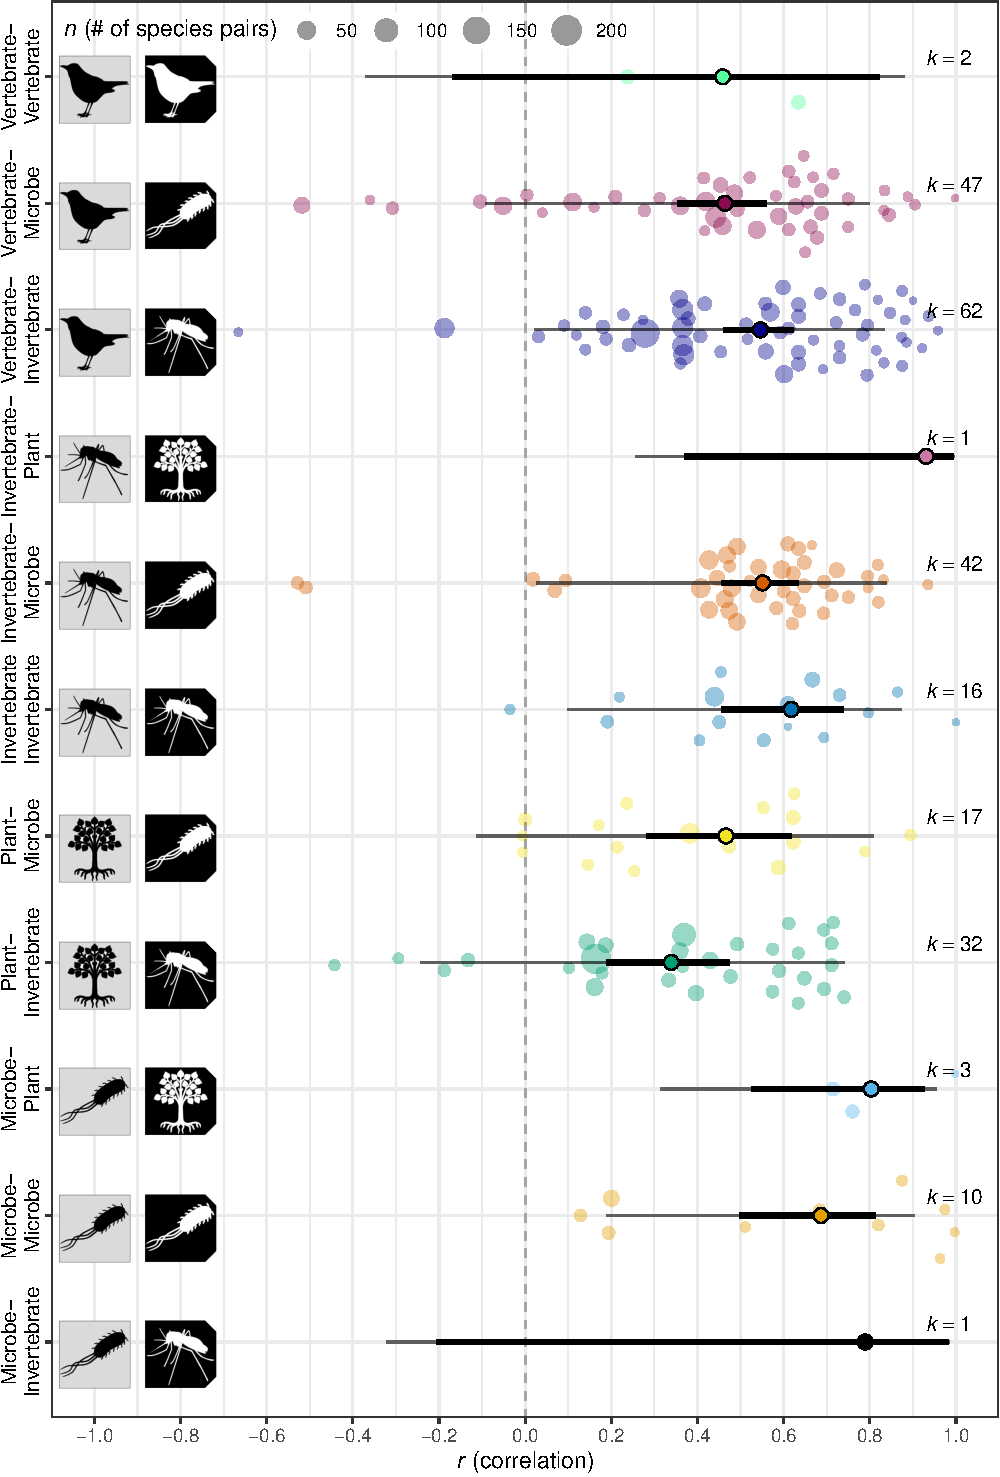
\includegraphics{Supporting_Information_files/figure-latex/unnamed-chunk-47-1.pdf}

\textbf{Supplementary Figure 4:} A forest plot showing the group-wise
means (the categorical variable \texttt{host\_symbiont\_tax}) with their
95\% confidence intervals (thick lines) and 95\% prediction intervals
(thin lines), with observed effect sizes based on various sample sizes.

\hypertarget{model-selection-multi-predictor-model}{%
\subsubsection{Model selection (multi-predictor
model)}\label{model-selection-multi-predictor-model}}

Here we build the best model via an AICc based model selection method
implemented in the R package \texttt{MuMin}(Barton
\protect\hyperlink{ref-barton2009mumin}{2009}). For the full model, we
had 6 variables: \texttt{symbiosis}, \texttt{host\_tax\_broad},
\texttt{symbiont\_tax\_broad}, \texttt{mode\_of\_transmission\_broad},
\texttt{endo\_or\_ecto}, \& \texttt{log(host\_range\_link\_ratio)}. We
did not use \texttt{log(host\_range\_taxonomic\_breadth)} as it is
co-linear with \texttt{log(host\_range\_link\_ratio)} and also many of
the interaction terms.

\begin{Shaded}
\begin{Highlighting}[]
\CommentTok{# creates a new function to run in MuMIn}
\NormalTok{updated.rma.mv <-}\StringTok{ }\KeywordTok{updateable}\NormalTok{(rma.mv)}
\CommentTok{# updated.rma.mv}

\CommentTok{# testing the new function use method = 'ML' so that we can compare AIC}
\NormalTok{mr_full <-}\StringTok{ }\KeywordTok{updated.rma.mv}\NormalTok{(}\DataTypeTok{yi =}\NormalTok{ Zr, }\DataTypeTok{V =}\NormalTok{ VZr, }\DataTypeTok{mods =} \OperatorTok{~}\NormalTok{symbiosis }\OperatorTok{+}\StringTok{ }\NormalTok{host_tax_broad }\OperatorTok{+}\StringTok{ }
\StringTok{    }\NormalTok{symbiont_tax_broad }\OperatorTok{+}\StringTok{ }\NormalTok{mode_of_transmission_broad }\OperatorTok{+}\StringTok{ }\NormalTok{endo_or_ecto }\OperatorTok{+}\StringTok{ }\KeywordTok{log}\NormalTok{(host_range_link_ratio), }
    \DataTypeTok{test =} \StringTok{"t"}\NormalTok{, }\DataTypeTok{random =} \OperatorTok{~}\DecValTok{1} \OperatorTok{|}\StringTok{ }\NormalTok{authors, }\DataTypeTok{method =} \StringTok{"ML"}\NormalTok{, }\DataTypeTok{data =}\NormalTok{ dat)}

\CommentTok{# ============================= additional methods for 'rma.mv' class (made by}
\CommentTok{# Kamil Barton) we need this to run model selection with rma.mv in MuMIn}
\CommentTok{# =============================}
\NormalTok{formula.rma.mv <-}\StringTok{ }\ControlFlowTok{function}\NormalTok{(x, ...) }\KeywordTok{return}\NormalTok{(}\KeywordTok{eval}\NormalTok{(}\KeywordTok{getCall}\NormalTok{(x)}\OperatorTok{$}\NormalTok{mods))}

\NormalTok{makeArgs.rma.mv <-}\StringTok{ }\ControlFlowTok{function}\NormalTok{(obj, termNames, comb, opt, ...) \{}
\NormalTok{    ret <-}\StringTok{ }\NormalTok{MuMIn}\OperatorTok{:::}\KeywordTok{makeArgs.default}\NormalTok{(obj, termNames, comb, opt)}
    \KeywordTok{names}\NormalTok{(ret)[1L] <-}\StringTok{ "mods"}
\NormalTok{    ret}
\NormalTok{\}}

\NormalTok{nobs.rma.mv <-}\StringTok{ }\ControlFlowTok{function}\NormalTok{(object, ...) }\KeywordTok{attr}\NormalTok{(}\KeywordTok{logLik}\NormalTok{(object), }\StringTok{"nall"}\NormalTok{)}

\NormalTok{coefTable.rma.mv <-}\StringTok{ }\ControlFlowTok{function}\NormalTok{(model, ...) MuMIn}\OperatorTok{:::}\KeywordTok{.makeCoefTable}\NormalTok{(model}\OperatorTok{$}\NormalTok{b, model}\OperatorTok{$}\NormalTok{se, }
    \DataTypeTok{coefNames =} \KeywordTok{rownames}\NormalTok{(model}\OperatorTok{$}\NormalTok{b))}
\CommentTok{# =============================}

\CommentTok{# testing dredge dredge(full.model, evaluate=F) # show all candidate models n =}
\CommentTok{# 32 model exisit}
\NormalTok{candidates <-}\StringTok{ }\KeywordTok{dredge}\NormalTok{(mr_full)}

\CommentTok{# displays delta AICc <2}
\NormalTok{candidates_aic2 <-}\StringTok{ }\KeywordTok{subset}\NormalTok{(candidates, delta }\OperatorTok{<}\StringTok{ }\DecValTok{2}\NormalTok{)}

\CommentTok{# model averaging it seems like models are using z values rather than t values}
\CommentTok{# (which will be OK)}
\NormalTok{mr_averaged_aic2 <-}\StringTok{ }\KeywordTok{summary}\NormalTok{(}\KeywordTok{model.avg}\NormalTok{(candidates, delta }\OperatorTok{<}\StringTok{ }\DecValTok{2}\NormalTok{))}

\CommentTok{# relative importance of each predictor}
\NormalTok{importance <-}\StringTok{ }\KeywordTok{importance}\NormalTok{(candidates)}

\CommentTok{# use REML if not for model comparision}
\NormalTok{model1 <-}\StringTok{ }\KeywordTok{rma.mv}\NormalTok{(}\DataTypeTok{yi =}\NormalTok{ Zr, }\DataTypeTok{V =}\NormalTok{ VZr, }\DataTypeTok{mods =} \OperatorTok{~}\NormalTok{host_tax_broad }\OperatorTok{+}\StringTok{ }\KeywordTok{log}\NormalTok{(host_range_link_ratio) }\OperatorTok{+}\StringTok{ }
\StringTok{    }\NormalTok{mode_of_transmission_broad }\OperatorTok{+}\StringTok{ }\NormalTok{symbiosis, }\DataTypeTok{test =} \StringTok{"t"}\NormalTok{, }\DataTypeTok{random =} \OperatorTok{~}\DecValTok{1} \OperatorTok{|}\StringTok{ }\NormalTok{authors, }\DataTypeTok{method =} \StringTok{"REML"}\NormalTok{, }
    \DataTypeTok{data =}\NormalTok{ dat)}
\NormalTok{model2 <-}\StringTok{ }\KeywordTok{rma.mv}\NormalTok{(}\DataTypeTok{yi =}\NormalTok{ Zr, }\DataTypeTok{V =}\NormalTok{ VZr, }\DataTypeTok{mods =} \OperatorTok{~}\NormalTok{host_tax_broad }\OperatorTok{+}\StringTok{ }\KeywordTok{log}\NormalTok{(host_range_link_ratio) }\OperatorTok{+}\StringTok{ }
\StringTok{    }\NormalTok{mode_of_transmission_broad, }\DataTypeTok{test =} \StringTok{"t"}\NormalTok{, }\DataTypeTok{random =} \OperatorTok{~}\DecValTok{1} \OperatorTok{|}\StringTok{ }\NormalTok{authors, }\DataTypeTok{method =} \StringTok{"REML"}\NormalTok{, }
    \DataTypeTok{data =}\NormalTok{ dat)}
\NormalTok{model3 <-}\StringTok{ }\KeywordTok{rma.mv}\NormalTok{(}\DataTypeTok{yi =}\NormalTok{ Zr, }\DataTypeTok{V =}\NormalTok{ VZr, }\DataTypeTok{mods =} \OperatorTok{~}\NormalTok{host_tax_broad }\OperatorTok{+}\StringTok{ }\NormalTok{mode_of_transmission_broad }\OperatorTok{+}\StringTok{ }
\StringTok{    }\NormalTok{symbiosis, }\DataTypeTok{test =} \StringTok{"t"}\NormalTok{, }\DataTypeTok{random =} \OperatorTok{~}\DecValTok{1} \OperatorTok{|}\StringTok{ }\NormalTok{authors, }\DataTypeTok{method =} \StringTok{"REML"}\NormalTok{, }\DataTypeTok{data =}\NormalTok{ dat)}
\NormalTok{model4 <-}\StringTok{ }\KeywordTok{rma.mv}\NormalTok{(}\DataTypeTok{yi =}\NormalTok{ Zr, }\DataTypeTok{V =}\NormalTok{ VZr, }\DataTypeTok{mods =} \OperatorTok{~}\NormalTok{host_tax_broad }\OperatorTok{+}\StringTok{ }\NormalTok{mode_of_transmission_broad, }
    \DataTypeTok{test =} \StringTok{"t"}\NormalTok{, }\DataTypeTok{random =} \OperatorTok{~}\DecValTok{1} \OperatorTok{|}\StringTok{ }\NormalTok{authors, }\DataTypeTok{method =} \StringTok{"REML"}\NormalTok{, }\DataTypeTok{data =}\NormalTok{ dat)}
\end{Highlighting}
\end{Shaded}

\textbf{Supplementary Table 13:} The top 2 models (out of 32 possible
models) within the \(\Delta\)AIC difference of 2, and which 6 variables:
\texttt{symbiosis}, \texttt{host\_tax\_broad},
\texttt{symbiont\_tax\_broad}, \texttt{mode\_of\_transmission\_broad},
\texttt{endo\_or\_ecto}, \& \texttt{log(host\_range\_link\_ratio)} were
included (indicated by \(+\)); model weights (for the 2 models) and the
sum of weights for each of the variables (from the 32 models) are
included.

\begin{Shaded}
\begin{Highlighting}[]
\CommentTok{# creating a table}
\KeywordTok{tibble}\NormalTok{(}\StringTok{`}\DataTypeTok{Model (variable weight)}\StringTok{`}\NormalTok{ =}\StringTok{ }\KeywordTok{c}\NormalTok{(}\StringTok{"Model1"}\NormalTok{, }\StringTok{"Model2"}\NormalTok{, }\StringTok{"Model3"}\NormalTok{, }\StringTok{"Model4"}\NormalTok{, }\StringTok{"(Sum of weights)"}\NormalTok{), }
    \DataTypeTok{transmission =} \KeywordTok{c}\NormalTok{(}\KeywordTok{if_else}\NormalTok{(candidates_aic2}\OperatorTok{$}\NormalTok{mode_of_transmission_broad }\OperatorTok{==}\StringTok{ "+"}\NormalTok{, }\StringTok{"$+$"}\NormalTok{, }
        \StringTok{"NA"}\NormalTok{), }\KeywordTok{round}\NormalTok{(importance[}\DecValTok{1}\NormalTok{], }\DecValTok{3}\NormalTok{)), }\DataTypeTok{host_tax =} \KeywordTok{c}\NormalTok{(}\KeywordTok{if_else}\NormalTok{(candidates_aic2}\OperatorTok{$}\NormalTok{host_tax_broad }\OperatorTok{==}\StringTok{ }
\StringTok{        "+"}\NormalTok{, }\StringTok{"$+$"}\NormalTok{, }\StringTok{"NA"}\NormalTok{), }\KeywordTok{round}\NormalTok{(importance[}\DecValTok{2}\NormalTok{], }\DecValTok{3}\NormalTok{)), }\DataTypeTok{symbiosis =} \KeywordTok{c}\NormalTok{(}\KeywordTok{if_else}\NormalTok{(candidates_aic2}\OperatorTok{$}\NormalTok{symbiosis }\OperatorTok{==}\StringTok{ }
\StringTok{        "+"}\NormalTok{, }\StringTok{"$+$"}\NormalTok{, }\StringTok{"NA"}\NormalTok{), }\KeywordTok{round}\NormalTok{(importance[}\DecValTok{3}\NormalTok{], }\DecValTok{3}\NormalTok{)), }\DataTypeTok{host_range =} \KeywordTok{c}\NormalTok{(}\KeywordTok{if_else}\NormalTok{(candidates_aic2}\OperatorTok{$}\StringTok{`}\DataTypeTok{log(host_range_link_ratio)}\StringTok{`} \OperatorTok{>=}\StringTok{ }
\StringTok{        }\DecValTok{0}\NormalTok{, }\StringTok{"$+$"}\NormalTok{, }\StringTok{"NA"}\NormalTok{), }\KeywordTok{round}\NormalTok{(importance[}\DecValTok{4}\NormalTok{], }\DecValTok{3}\NormalTok{)), }\DataTypeTok{symbiont_tax =} \KeywordTok{c}\NormalTok{(}\KeywordTok{if_else}\NormalTok{(candidates_aic2}\OperatorTok{$}\NormalTok{symbiont_tax_broad }\OperatorTok{==}\StringTok{ }
\StringTok{        "+"}\NormalTok{, }\StringTok{"$+$"}\NormalTok{, }\StringTok{"NA"}\NormalTok{), }\KeywordTok{round}\NormalTok{(importance[}\DecValTok{5}\NormalTok{], }\DecValTok{3}\NormalTok{)), }\DataTypeTok{endo_or_ecto =} \KeywordTok{c}\NormalTok{(}\KeywordTok{if_else}\NormalTok{(candidates_aic2}\OperatorTok{$}\NormalTok{endo_or_ecto }\OperatorTok{==}\StringTok{ }
\StringTok{        "+"}\NormalTok{, }\StringTok{"$+$"}\NormalTok{, }\StringTok{"NA"}\NormalTok{), }\KeywordTok{round}\NormalTok{(importance[}\DecValTok{6}\NormalTok{], }\DecValTok{3}\NormalTok{)), }\DataTypeTok{delta_AICc =} \KeywordTok{c}\NormalTok{(candidates_aic2}\OperatorTok{$}\NormalTok{delta, }
        \OtherTok{NA}\NormalTok{), }\DataTypeTok{Weight =} \KeywordTok{c}\NormalTok{(candidates_aic2}\OperatorTok{$}\NormalTok{weight, }\OtherTok{NA}\NormalTok{)) }\OperatorTok\StringTok{ }\KeywordTok{kable}\NormalTok{(}\StringTok{"html"}\NormalTok{, }\DataTypeTok{digits =} \DecValTok{3}\NormalTok{) }\OperatorTok\StringTok{ }
\StringTok{    }\KeywordTok{kable_styling}\NormalTok{(}\StringTok{"striped"}\NormalTok{, }\DataTypeTok{position =} \StringTok{"left"}\NormalTok{)}
\end{Highlighting}
\end{Shaded}

Model (variable weight)

transmission

host\_tax

symbiosis

host\_range

symbiont\_tax

endo\_or\_ecto

delta\_AICc

Weight

Model1

\(+\)

\(+\)

\(+\)

\(+\)

NA

NA

0.000

0.266

Model2

\(+\)

\(+\)

NA

\(+\)

NA

NA

0.088

0.255

Model3

\(+\)

\(+\)

\(+\)

NA

NA

NA

0.114

0.252

Model4

\(+\)

\(+\)

NA

NA

NA

NA

0.321

0.227

(Sum of weights)

0.999

0.794

0.497

0.486

0.163

0.129

NA

NA

\hypertarget{model-averaging}{%
\paragraph{Model averaging}\label{model-averaging}}

\textbf{Supplementary Table 14:} The average estimates for regression
coefficients (Estimate), 95\% confidence intervals (CIs), variance
components (V) and variance explained,
\emph{R}\textsuperscript{2}\textsubscript{{[}marginal{]}} (R2) from the
2 best meta-regression models.

\begin{Shaded}
\begin{Highlighting}[]
\CommentTok{# getting averaged R2 and variance components not provided by the MuMIn package}
\NormalTok{average_sigma2 <-}\StringTok{ }\KeywordTok{weighted.mean}\NormalTok{(}\DataTypeTok{x =} \KeywordTok{c}\NormalTok{(model1}\OperatorTok{$}\NormalTok{sigma2, model2}\OperatorTok{$}\NormalTok{sigma2, model3}\OperatorTok{$}\NormalTok{sigma2, }
\NormalTok{    model4}\OperatorTok{$}\NormalTok{sigma2), }\DataTypeTok{w =}\NormalTok{ candidates_aic2}\OperatorTok{$}\NormalTok{weight)}
\NormalTok{average_R2 <-}\StringTok{ }\KeywordTok{weighted.mean}\NormalTok{(}\DataTypeTok{x =} \KeywordTok{c}\NormalTok{(}\KeywordTok{R2}\NormalTok{(model1)[}\DecValTok{1}\NormalTok{], }\KeywordTok{R2}\NormalTok{(model2)[}\DecValTok{1}\NormalTok{], }\KeywordTok{R2}\NormalTok{(model3)[}\DecValTok{1}\NormalTok{], }\KeywordTok{R2}\NormalTok{(model4)[}\DecValTok{1}\NormalTok{]), }
    \DataTypeTok{w =}\NormalTok{ candidates_aic2}\OperatorTok{$}\NormalTok{weight)}

\CommentTok{# creating a table}
\KeywordTok{tibble}\NormalTok{(}\StringTok{`}\DataTypeTok{Fixed effect}\StringTok{`}\NormalTok{ =}\StringTok{ }\KeywordTok{c}\NormalTok{(}\StringTok{"Intercept (both-Microbe-Mutulist)"}\NormalTok{, }\StringTok{"Microbe-Plant"}\NormalTok{, }\StringTok{"Microbe-Invert"}\NormalTok{, }
    \StringTok{"Microbe-Vert"}\NormalTok{, }\StringTok{"host_range"}\NormalTok{, }\StringTok{"both-horizontal"}\NormalTok{, }\StringTok{"both-vertical"}\NormalTok{, }\StringTok{"Mutulist-Parasite"}\NormalTok{), }
    \DataTypeTok{Estimate =}\NormalTok{ mr_averaged_aic2}\OperatorTok{$}\NormalTok{coefmat.full[, }\DecValTok{1}\NormalTok{], }\StringTok{`}\DataTypeTok{Lower CI [0.025]}\StringTok{`}\NormalTok{ =}\StringTok{ }\NormalTok{mr_averaged_aic2}\OperatorTok{$}\NormalTok{coefmat.full[, }
        \DecValTok{1}\NormalTok{] }\OperatorTok{-}\StringTok{ }\NormalTok{mr_averaged_aic2}\OperatorTok{$}\NormalTok{coefmat.full[, }\DecValTok{2}\NormalTok{] }\OperatorTok{*}\StringTok{ }\KeywordTok{qnorm}\NormalTok{(}\FloatTok{0.975}\NormalTok{), }\StringTok{`}\DataTypeTok{Upper CI  [0.975]}\StringTok{`}\NormalTok{ =}\StringTok{ }\NormalTok{mr_averaged_aic2}\OperatorTok{$}\NormalTok{coefmat.full[, }
        \DecValTok{1}\NormalTok{] }\OperatorTok{+}\StringTok{ }\NormalTok{mr_averaged_aic2}\OperatorTok{$}\NormalTok{coefmat.full[, }\DecValTok{2}\NormalTok{] }\OperatorTok{*}\StringTok{ }\KeywordTok{qnorm}\NormalTok{(}\FloatTok{0.975}\NormalTok{), }\StringTok{`}\DataTypeTok{V[authors]}\StringTok{`}\NormalTok{ =}\StringTok{ }\KeywordTok{c}\NormalTok{(average_sigma2, }
        \KeywordTok{rep}\NormalTok{(}\OtherTok{NA}\NormalTok{, }\DecValTok{7}\NormalTok{)), }\DataTypeTok{R2 =} \KeywordTok{c}\NormalTok{(average_R2, }\KeywordTok{rep}\NormalTok{(}\OtherTok{NA}\NormalTok{, }\DecValTok{7}\NormalTok{))) }\OperatorTok\StringTok{ }\KeywordTok{kable}\NormalTok{(}\StringTok{"html"}\NormalTok{, }\DataTypeTok{digits =} \DecValTok{3}\NormalTok{) }\OperatorTok\StringTok{ }
\StringTok{    }\KeywordTok{kable_styling}\NormalTok{(}\StringTok{"striped"}\NormalTok{, }\DataTypeTok{position =} \StringTok{"left"}\NormalTok{)}
\end{Highlighting}
\end{Shaded}

Fixed effect

Estimate

Lower CI {[}0.025{]}

Upper CI {[}0.975{]}

V{[}authors{]}

R2

Intercept (both-Microbe-Mutulist)

0.902

0.628

1.177

0.071

0.23

Microbe-Plant

-0.428

-0.711

-0.146

NA

NA

Microbe-Invert

-0.320

-0.601

-0.039

NA

NA

Microbe-Vert

-0.273

-0.538

-0.009

NA

NA

host\_range

0.045

-0.098

0.188

NA

NA

both-horizontal

-0.076

-0.223

0.071

NA

NA

both-vertical

0.155

-0.100

0.409

NA

NA

Mutulist-Parasite

-0.037

-0.186

0.112

NA

NA

\hypertarget{publication-bias-analysis}{%
\subsection{Publication Bias Analysis}\label{publication-bias-analysis}}

Here, we conducted 3 kinds of publication bias analyses: 1)
contour-enhanced funnel plots (Peters \emph{et al.}
\protect\hyperlink{ref-peters2008contour}{2008}) of residuals (Egger
\emph{et al.} \protect\hyperlink{ref-egger1997bias}{1997}; Nakagawa \&
Santos \protect\hyperlink{ref-nakagawa2012methodological}{2012}), 2) a
type of Egger regression (Egger \emph{et al.}
\protect\hyperlink{ref-egger1997bias}{1997}; Moreno \emph{et al.}
\protect\hyperlink{ref-moreno2009assessment}{2009}), and 3) a
regression-based time-lag bias test (Nakagawa \& Santos
\protect\hyperlink{ref-nakagawa2012methodological}{2012}).

\hypertarget{funnel-plot}{%
\subsubsection{Funnel plot}\label{funnel-plot}}

A normal funnel plot assumes homogeneity (i.e.,
\emph{I}\textsuperscript{2} = 0). Therefore, we controlled for important
moderators (i.e., \texttt{mode\_of\_transmission\_broad},
\texttt{host\_tax\_broad}, \texttt{log(host\_range\_link\_ratio)}, \&
\texttt{symbiosis}).

\hypertarget{residual-funnel-plot-1}{%
\paragraph{Residual funnel plot 1}\label{residual-funnel-plot-1}}

We do not observe normal skewness in our enhanced-counter funnel plot
(\textbf{Supplementary Figure 5}). This funnel asymmetry seems different
from one cased by publication bias(Peters \emph{et al.}
\protect\hyperlink{ref-peters2008contour}{2008}); we do not expect a
``hollow'' in the region with high precision or i.e.~inverse standard
error (2.4-4) and relative high effect sizes (\emph{Zr} = 0.5-1.0). The
funnel asymmetry is mainly caused by the boundary created by the number
of randomizations (see the ``Sensitivity Analysis'' section where we
deal with this skewness).

\begin{Shaded}
\begin{Highlighting}[]
\CommentTok{# }
\NormalTok{res_funnel_plot <-}\StringTok{ }\KeywordTok{rma.mv}\NormalTok{(}\DataTypeTok{yi =}\NormalTok{ Zr, }\DataTypeTok{V =}\NormalTok{ VZr, }\DataTypeTok{mods =} \OperatorTok{~}\NormalTok{mode_of_transmission_broad }\OperatorTok{+}\StringTok{ }
\StringTok{    }\NormalTok{host_tax_broad }\OperatorTok{+}\StringTok{ }\KeywordTok{log}\NormalTok{(host_range_link_ratio) }\OperatorTok{+}\StringTok{ }\NormalTok{symbiosis, }\DataTypeTok{random =} \OperatorTok{~}\DecValTok{1} \OperatorTok{|}\StringTok{ }\NormalTok{authors, }
    \DataTypeTok{data =}\NormalTok{ dat)}

\KeywordTok{funnel}\NormalTok{(res_funnel_plot, }\DataTypeTok{yaxis =} \StringTok{"seinv"}\NormalTok{, }\DataTypeTok{level =} \KeywordTok{c}\NormalTok{(}\DecValTok{90}\NormalTok{, }\DecValTok{95}\NormalTok{, }\DecValTok{99}\NormalTok{), }\DataTypeTok{shade =} \KeywordTok{c}\NormalTok{(}\StringTok{"white"}\NormalTok{, }
    \StringTok{"gray55"}\NormalTok{, }\StringTok{"gray75"}\NormalTok{), }\DataTypeTok{refline =} \DecValTok{0}\NormalTok{, }\DataTypeTok{legend =} \OtherTok{TRUE}\NormalTok{)}
\end{Highlighting}
\end{Shaded}

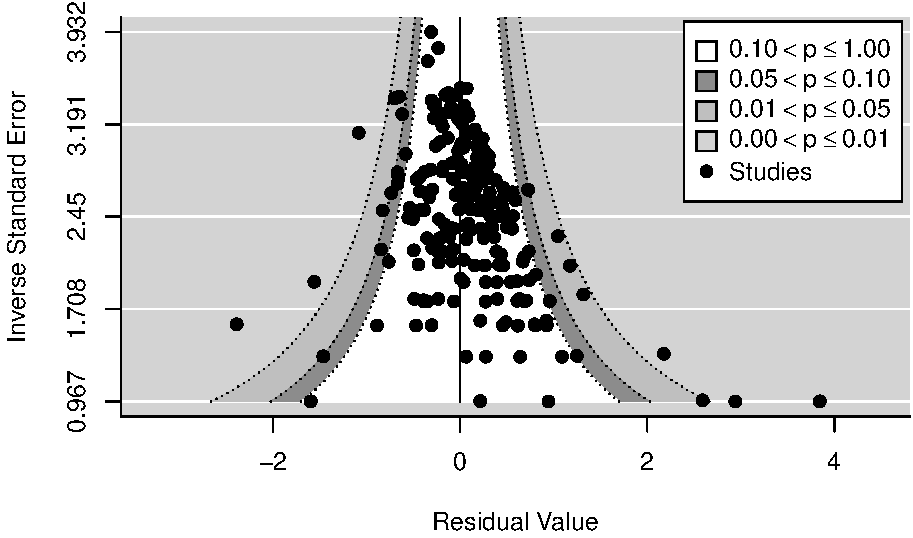
\includegraphics{Supporting_Information_files/figure-latex/unnamed-chunk-51-1.pdf}

\textbf{Supplementary Figure 5:} A residual funnel plot from the
meta-regression model with \texttt{mode\_of\_transmission\_broad},
\texttt{host\_tax\_broad}, \& \texttt{symbiosis}; `residual value' is on
\emph{Zr} and `inverse standard error' is precision
\texttt{1/sqrt(VZr)}.

\hypertarget{residual-funnel-plot-2}{%
\paragraph{Residual funnel plot 2}\label{residual-funnel-plot-2}}

Further, Egger regression analyses (see below) showed that
\texttt{sqrt(VZr)} (sampling errors {[}SE{]} for effect sizes) accounts
much heterogeneity, so we added that to our model. The funnel asymmetry
we see in \textbf{Supplementary Figure 6} (if any) is much less severe
than that in \textbf{Supplementary Figure 5}.

\begin{Shaded}
\begin{Highlighting}[]
\CommentTok{# }
\NormalTok{res_funnel_plot2 <-}\StringTok{ }\KeywordTok{rma.mv}\NormalTok{(}\DataTypeTok{yi =}\NormalTok{ Zr, }\DataTypeTok{V =}\NormalTok{ VZr, }\DataTypeTok{mods =} \OperatorTok{~}\KeywordTok{sqrt}\NormalTok{(VZr) }\OperatorTok{+}\StringTok{ }\NormalTok{mode_of_transmission_broad }\OperatorTok{+}\StringTok{ }
\StringTok{    }\NormalTok{host_tax_broad }\OperatorTok{+}\StringTok{ }\KeywordTok{log}\NormalTok{(host_range_link_ratio) }\OperatorTok{+}\StringTok{ }\NormalTok{symbiosis, }\DataTypeTok{random =} \OperatorTok{~}\DecValTok{1} \OperatorTok{|}\StringTok{ }\NormalTok{authors, }
    \DataTypeTok{data =}\NormalTok{ dat)}

\KeywordTok{funnel}\NormalTok{(res_funnel_plot2, }\DataTypeTok{yaxis =} \StringTok{"seinv"}\NormalTok{, }\DataTypeTok{level =} \KeywordTok{c}\NormalTok{(}\DecValTok{90}\NormalTok{, }\DecValTok{95}\NormalTok{, }\DecValTok{99}\NormalTok{), }\DataTypeTok{shade =} \KeywordTok{c}\NormalTok{(}\StringTok{"white"}\NormalTok{, }
    \StringTok{"gray55"}\NormalTok{, }\StringTok{"gray75"}\NormalTok{), }\DataTypeTok{refline =} \DecValTok{0}\NormalTok{, }\DataTypeTok{legend =} \OtherTok{TRUE}\NormalTok{)}
\end{Highlighting}
\end{Shaded}

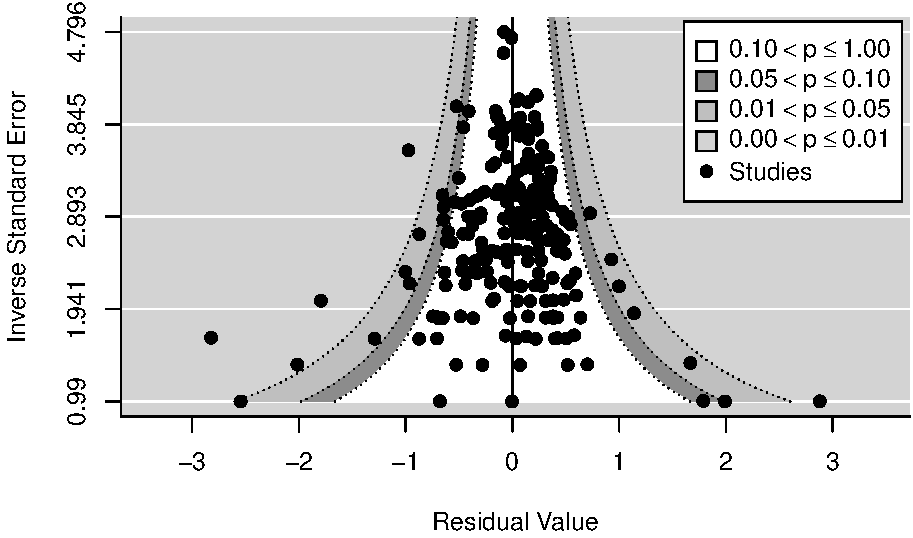
\includegraphics{Supporting_Information_files/figure-latex/unnamed-chunk-52-1.pdf}

\textbf{Supplementary Figure 6:} A residual funnel plot from the
meta-regression model with \texttt{sqrt(VZr)},
\texttt{mode\_of\_transmission\_broad}, \texttt{host\_tax\_broad},
\texttt{log(host\_range\_link\_ratio)}, \& \texttt{symbiosis}; `residual
value' is on \emph{Zr} and `inverse standard error' is precision
\texttt{1/sqrt(VZr)}.

\hypertarget{egger-regression}{%
\subsubsection{Egger regression}\label{egger-regression}}

We applied Egger regression to test whether the funnel asymmetries we
observe in our funnel plots are statistical significant or not.

\hypertarget{univariate-egger-regression}{%
\paragraph{Univariate Egger
regression}\label{univariate-egger-regression}}

The test (or \texttt{sqrt(VZr)}) is significant. However, as mentioned
above, this is due to the boundary created by the number of
randomizations; this boundary can be seen in \textbf{Supplementary
Figure 7}

\begin{Shaded}
\begin{Highlighting}[]
\CommentTok{# }
\NormalTok{egger_regression_uni <-}\StringTok{ }\KeywordTok{rma.mv}\NormalTok{(}\DataTypeTok{yi =}\NormalTok{ Zr, }\DataTypeTok{V =}\NormalTok{ VZr, }\DataTypeTok{mods =} \OperatorTok{~}\KeywordTok{sqrt}\NormalTok{(VZr), }\DataTypeTok{random =} \OperatorTok{~}\DecValTok{1} \OperatorTok{|}\StringTok{ }
\StringTok{    }\NormalTok{authors, }\DataTypeTok{data =}\NormalTok{ dat)}
\end{Highlighting}
\end{Shaded}

\textbf{Supplementary Table 15:} Regression coefficients (Estimate),
95\% confidence intervals (CIs), variance components (V) and variance
explained, \emph{R}\textsuperscript{2}\textsubscript{{[}marginal{]}}
(R2) from the meta-regression with \texttt{sqrt(VZr)}.

\begin{Shaded}
\begin{Highlighting}[]
\CommentTok{# getting marginal R2}
\NormalTok{r2_egger_regression_uni <-}\StringTok{ }\KeywordTok{R2}\NormalTok{(egger_regression_uni)}

\CommentTok{# getting estimates: name does not work for slopes}
\NormalTok{res_egger_regression_uni <-}\StringTok{ }\KeywordTok{get_est}\NormalTok{(egger_regression_uni, }\DataTypeTok{mod =} \StringTok{"sqrt(VZr)"}\NormalTok{)}

\CommentTok{# creating a table}
\KeywordTok{tibble}\NormalTok{(}\StringTok{`}\DataTypeTok{Fixed effect}\StringTok{`}\NormalTok{ =}\StringTok{ }\KeywordTok{c}\NormalTok{(}\StringTok{"Intercept"}\NormalTok{, }\StringTok{"sqrt(VZr)"}\NormalTok{), }\DataTypeTok{Estimate =} \KeywordTok{c}\NormalTok{(res_egger_regression_uni}\OperatorTok{$}\NormalTok{estimate), }
    \StringTok{`}\DataTypeTok{Lower CI [0.025]}\StringTok{`}\NormalTok{ =}\StringTok{ }\KeywordTok{c}\NormalTok{(res_egger_regression_uni}\OperatorTok{$}\NormalTok{lowerCL), }\StringTok{`}\DataTypeTok{Upper CI  [0.975]}\StringTok{`}\NormalTok{ =}\StringTok{ }\KeywordTok{c}\NormalTok{(res_egger_regression_uni}\OperatorTok{$}\NormalTok{upperCL), }
    \StringTok{`}\DataTypeTok{V[authors]}\StringTok{`}\NormalTok{ =}\StringTok{ }\KeywordTok{c}\NormalTok{(egger_regression_uni}\OperatorTok{$}\NormalTok{sigma2, }\OtherTok{NA}\NormalTok{), }\DataTypeTok{R2 =} \KeywordTok{c}\NormalTok{(r2_egger_regression_uni[}\DecValTok{1}\NormalTok{], }
        \OtherTok{NA}\NormalTok{)) }\OperatorTok\StringTok{ }\KeywordTok{kable}\NormalTok{(}\StringTok{"html"}\NormalTok{, }\DataTypeTok{digits =} \DecValTok{3}\NormalTok{) }\OperatorTok\StringTok{ }\KeywordTok{kable_styling}\NormalTok{(}\StringTok{"striped"}\NormalTok{, }\DataTypeTok{position =} \StringTok{"left"}\NormalTok{)}
\end{Highlighting}
\end{Shaded}

Fixed effect

Estimate

Lower CI {[}0.025{]}

Upper CI {[}0.975{]}

V{[}authors{]}

R2

Intercept

0.217

0.093

0.342

0.065

0.437

sqrt(VZr)

1.294

0.874

1.715

NA

NA

\begin{Shaded}
\begin{Highlighting}[]
\NormalTok{pred_egger_regression_uni <-}\StringTok{ }\KeywordTok{predict.rma}\NormalTok{(egger_regression_uni)}

\CommentTok{# plotting}

\NormalTok{fit_egger_regression_uni <-}\StringTok{ }\NormalTok{dat }\OperatorTok\StringTok{ }\KeywordTok{mutate}\NormalTok{(}\DataTypeTok{ymin =}\NormalTok{ pred_egger_regression_uni}\OperatorTok{$}\NormalTok{ci.lb, }
    \DataTypeTok{ymax =}\NormalTok{ pred_egger_regression_uni}\OperatorTok{$}\NormalTok{ci.ub, }\DataTypeTok{ymin2 =}\NormalTok{ pred_egger_regression_uni}\OperatorTok{$}\NormalTok{cr.lb, }
    \DataTypeTok{ymax2 =}\NormalTok{ pred_egger_regression_uni}\OperatorTok{$}\NormalTok{cr.ub, }\DataTypeTok{pred =}\NormalTok{ pred_egger_regression_uni}\OperatorTok{$}\NormalTok{pred) }\OperatorTok\StringTok{ }
\StringTok{    }\KeywordTok{ggplot}\NormalTok{(}\KeywordTok{aes}\NormalTok{(}\DataTypeTok{x =} \KeywordTok{sqrt}\NormalTok{(VZr), }\DataTypeTok{y =}\NormalTok{ Zr, }\DataTypeTok{size =}\NormalTok{ (}\DecValTok{1}\OperatorTok{/}\NormalTok{VZr) }\OperatorTok{+}\StringTok{ }\DecValTok{3}\NormalTok{)) }\OperatorTok{+}\StringTok{ }\KeywordTok{geom_point}\NormalTok{(}\DataTypeTok{shape =} \DecValTok{21}\NormalTok{, }
    \DataTypeTok{fill =} \StringTok{"grey90"}\NormalTok{) }\OperatorTok{+}\StringTok{ }\CommentTok{# geom_ribbon(aes(ymin = ymin, ymax = ymax), fill = '#0072B2') + # not quite sure}
\CommentTok{# why this does not work}
\KeywordTok{geom_smooth}\NormalTok{(}\KeywordTok{aes}\NormalTok{(}\DataTypeTok{y =}\NormalTok{ ymin2), }\DataTypeTok{method =} \StringTok{"loess"}\NormalTok{, }\DataTypeTok{se =} \OtherTok{FALSE}\NormalTok{, }\DataTypeTok{lty =} \StringTok{"dotted"}\NormalTok{, }\DataTypeTok{lwd =} \FloatTok{0.25}\NormalTok{, }
    \DataTypeTok{colour =} \StringTok{"#0072B2"}\NormalTok{) }\OperatorTok{+}\StringTok{ }\KeywordTok{geom_smooth}\NormalTok{(}\KeywordTok{aes}\NormalTok{(}\DataTypeTok{y =}\NormalTok{ ymax2), }\DataTypeTok{method =} \StringTok{"loess"}\NormalTok{, }\DataTypeTok{se =} \OtherTok{FALSE}\NormalTok{, }
    \DataTypeTok{lty =} \StringTok{"dotted"}\NormalTok{, }\DataTypeTok{lwd =} \FloatTok{0.25}\NormalTok{, }\DataTypeTok{colour =} \StringTok{"#0072B2"}\NormalTok{) }\OperatorTok{+}\StringTok{ }\KeywordTok{geom_smooth}\NormalTok{(}\KeywordTok{aes}\NormalTok{(}\DataTypeTok{y =}\NormalTok{ ymin), }
    \DataTypeTok{method =} \StringTok{"loess"}\NormalTok{, }\DataTypeTok{se =} \OtherTok{FALSE}\NormalTok{, }\DataTypeTok{lty =} \StringTok{"dotted"}\NormalTok{, }\DataTypeTok{lwd =} \FloatTok{0.25}\NormalTok{, }\DataTypeTok{colour =} \StringTok{"#D55E00"}\NormalTok{) }\OperatorTok{+}\StringTok{ }
\StringTok{    }\KeywordTok{geom_smooth}\NormalTok{(}\KeywordTok{aes}\NormalTok{(}\DataTypeTok{y =}\NormalTok{ ymax), }\DataTypeTok{method =} \StringTok{"loess"}\NormalTok{, }\DataTypeTok{se =} \OtherTok{FALSE}\NormalTok{, }\DataTypeTok{lty =} \StringTok{"dotted"}\NormalTok{, }\DataTypeTok{lwd =} \FloatTok{0.25}\NormalTok{, }
        \DataTypeTok{colour =} \StringTok{"#D55E00"}\NormalTok{) }\OperatorTok{+}\StringTok{ }\KeywordTok{geom_smooth}\NormalTok{(}\KeywordTok{aes}\NormalTok{(}\DataTypeTok{y =}\NormalTok{ pred), }\DataTypeTok{method =} \StringTok{"loess"}\NormalTok{, }\DataTypeTok{se =} \OtherTok{FALSE}\NormalTok{, }
    \DataTypeTok{lty =} \StringTok{"dashed"}\NormalTok{, }\DataTypeTok{lwd =} \FloatTok{0.5}\NormalTok{, }\DataTypeTok{colour =} \StringTok{"black"}\NormalTok{) }\OperatorTok{+}\StringTok{ }\KeywordTok{ylim}\NormalTok{(}\OperatorTok{-}\DecValTok{1}\NormalTok{, }\DecValTok{2}\NormalTok{) }\OperatorTok{+}\StringTok{ }\KeywordTok{xlim}\NormalTok{(}\FloatTok{0.05}\NormalTok{, }\FloatTok{0.45}\NormalTok{) }\OperatorTok{+}\StringTok{ }
\StringTok{    }\CommentTok{# geom_abline(intercept = mr_host_range_link_ratio$beta[[1]], slope =}
\CommentTok{# mr_host_range_link_ratio$beta[[2]], alpha = 0.7, linetype = 'dashed', size =}
\CommentTok{# 0.5) +}
\KeywordTok{labs}\NormalTok{(}\DataTypeTok{x =} \StringTok{"sqrt(sampling variance)"}\NormalTok{, }\DataTypeTok{y =} \KeywordTok{expression}\NormalTok{(}\KeywordTok{paste}\NormalTok{(}\KeywordTok{italic}\NormalTok{(Zr), }\StringTok{" (effect size)"}\NormalTok{)), }
    \DataTypeTok{size =} \KeywordTok{expression}\NormalTok{(}\KeywordTok{paste}\NormalTok{(}\KeywordTok{italic}\NormalTok{(n), }\StringTok{" (# of species pairs)"}\NormalTok{))) }\OperatorTok{+}\StringTok{ }\KeywordTok{guides}\NormalTok{(}\DataTypeTok{fill =} \StringTok{"none"}\NormalTok{, }
    \DataTypeTok{colour =} \StringTok{"none"}\NormalTok{) }\OperatorTok{+}\StringTok{ }\CommentTok{# themses}
\KeywordTok{theme_bw}\NormalTok{() }\OperatorTok{+}\StringTok{ }\KeywordTok{theme}\NormalTok{(}\DataTypeTok{legend.position =} \KeywordTok{c}\NormalTok{(}\DecValTok{0}\NormalTok{, }\DecValTok{1}\NormalTok{), }\DataTypeTok{legend.justification =} \KeywordTok{c}\NormalTok{(}\DecValTok{0}\NormalTok{, }\DecValTok{1}\NormalTok{)) }\OperatorTok{+}\StringTok{ }\KeywordTok{theme}\NormalTok{(}\DataTypeTok{legend.direction =} \StringTok{"horizontal"}\NormalTok{) }\OperatorTok{+}\StringTok{ }
\StringTok{    }\CommentTok{# theme(legend.background = element_rect(fill = 'white', colour = 'black')) +}
\KeywordTok{theme}\NormalTok{(}\DataTypeTok{legend.background =} \KeywordTok{element_blank}\NormalTok{()) }\OperatorTok{+}\StringTok{ }\KeywordTok{theme}\NormalTok{(}\DataTypeTok{axis.text.y =} \KeywordTok{element_text}\NormalTok{(}\DataTypeTok{size =} \DecValTok{10}\NormalTok{, }
    \DataTypeTok{colour =} \StringTok{"black"}\NormalTok{, }\DataTypeTok{hjust =} \FloatTok{0.5}\NormalTok{, }\DataTypeTok{angle =} \DecValTok{90}\NormalTok{))}

\NormalTok{fit_egger_regression_uni}
\end{Highlighting}
\end{Shaded}

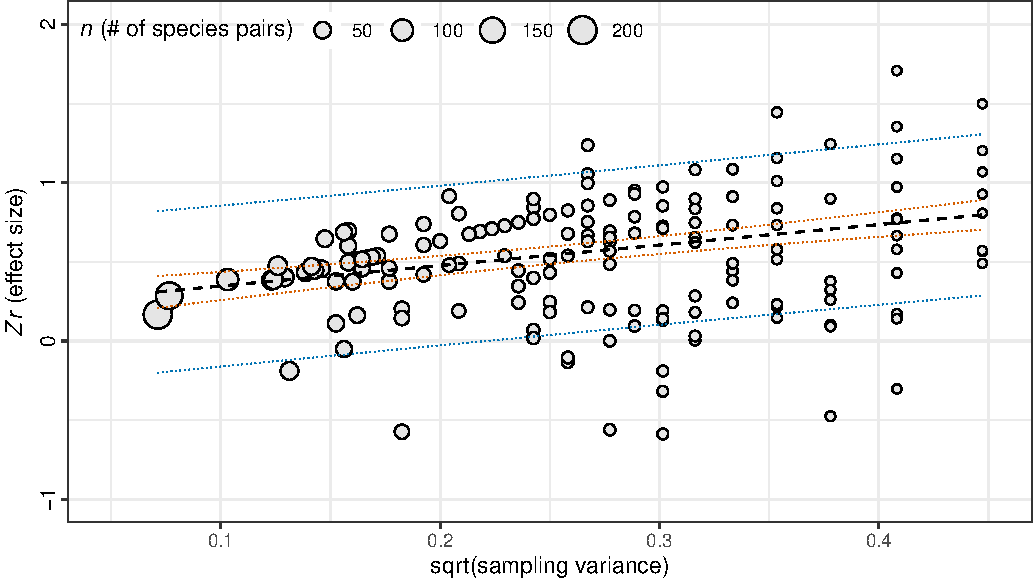
\includegraphics{Supporting_Information_files/figure-latex/unnamed-chunk-55-1.pdf}

\textbf{Supplementary Figure 7:} A bubble plot showing a predicted
regression line for the contentious variable \texttt{sqrt(VZr)},
indicating 95\% confidence regions (orange dotted lines) and 95\%
prediction regions (blue dotted lines), with observed effect sizes based
on various sample sizes.

\hypertarget{multivariate-egger-regression}{%
\paragraph{Multivariate Egger
regression}\label{multivariate-egger-regression}}

We also conducted a Egger regression controlling other important
moderators (i.e., \texttt{mode\_of\_transmission\_broad},
\texttt{host\_tax\_broad}, \texttt{log(host\_range\_link\_ratio)}, \&
\texttt{symbiosis}). After controlling for these variables,
\texttt{sqrt(VZr)} stays significant.

\begin{Shaded}
\begin{Highlighting}[]
\CommentTok{# }
\NormalTok{egger_regression_mul <-}\StringTok{ }\KeywordTok{rma.mv}\NormalTok{(}\DataTypeTok{yi =}\NormalTok{ Zr, }\DataTypeTok{V =}\NormalTok{ VZr, }\DataTypeTok{mods =} \OperatorTok{~}\KeywordTok{sqrt}\NormalTok{(VZr) }\OperatorTok{+}\StringTok{ }\NormalTok{mode_of_transmission_broad }\OperatorTok{+}\StringTok{ }
\StringTok{    }\NormalTok{host_tax_broad }\OperatorTok{+}\StringTok{ }\KeywordTok{log}\NormalTok{(host_range_link_ratio) }\OperatorTok{+}\StringTok{ }\NormalTok{symbiosis, }\DataTypeTok{random =} \OperatorTok{~}\DecValTok{1} \OperatorTok{|}\StringTok{ }\NormalTok{authors, }
    \DataTypeTok{data =}\NormalTok{ dat)}
\end{Highlighting}
\end{Shaded}

\textbf{Supplementary Table 16:} Regression coefficients (Estimate),
95\% confidence intervals (CIs), variance components (V) and variance
explained, \emph{R}\textsuperscript{2}\textsubscript{{[}marginal{]}}
(R2) from the meta-regression with \texttt{sqrt(VZr)}.

\begin{Shaded}
\begin{Highlighting}[]
\CommentTok{# getting marginal R2}
\NormalTok{r2_egger_regression_mul <-}\StringTok{ }\KeywordTok{R2}\NormalTok{(egger_regression_mul)}

\CommentTok{# creating a table}
\KeywordTok{tibble}\NormalTok{(}\StringTok{`}\DataTypeTok{Fixed effect}\StringTok{`}\NormalTok{ =}\StringTok{ }\KeywordTok{c}\NormalTok{(}\StringTok{"Intercept (both-Microbe-Mutulist)"}\NormalTok{, }\StringTok{"sqrt(VZr)"}\NormalTok{, }\StringTok{"both-horizontal"}\NormalTok{, }
    \StringTok{"both-vertical"}\NormalTok{, }\StringTok{"Microbe-Plant"}\NormalTok{, }\StringTok{"Microbe-Invert"}\NormalTok{, }\StringTok{"Microbe-Vert"}\NormalTok{, }\StringTok{"host_range"}\NormalTok{, }
    \StringTok{"Mutulist-Parasite"}\NormalTok{), }\DataTypeTok{Estimate =} \KeywordTok{c}\NormalTok{(egger_regression_mul}\OperatorTok{$}\NormalTok{b), }\StringTok{`}\DataTypeTok{Lower CI [0.025]}\StringTok{`}\NormalTok{ =}\StringTok{ }\KeywordTok{c}\NormalTok{(egger_regression_mul}\OperatorTok{$}\NormalTok{ci.lb), }
    \StringTok{`}\DataTypeTok{Upper CI  [0.975]}\StringTok{`}\NormalTok{ =}\StringTok{ }\KeywordTok{c}\NormalTok{(egger_regression_mul}\OperatorTok{$}\NormalTok{ci.ub), }\StringTok{`}\DataTypeTok{V[authors]}\StringTok{`}\NormalTok{ =}\StringTok{ }\KeywordTok{c}\NormalTok{(egger_regression_mul}\OperatorTok{$}\NormalTok{sigma2, }
        \KeywordTok{rep}\NormalTok{(}\OtherTok{NA}\NormalTok{, }\DecValTok{8}\NormalTok{)), }\DataTypeTok{R2 =} \KeywordTok{c}\NormalTok{(r2_egger_regression_mul[}\DecValTok{1}\NormalTok{], }\KeywordTok{rep}\NormalTok{(}\OtherTok{NA}\NormalTok{, }\DecValTok{8}\NormalTok{))) }\OperatorTok\StringTok{ }\KeywordTok{kable}\NormalTok{(}\StringTok{"html"}\NormalTok{, }
    \DataTypeTok{digits =} \DecValTok{3}\NormalTok{) }\OperatorTok\StringTok{ }\KeywordTok{kable_styling}\NormalTok{(}\StringTok{"striped"}\NormalTok{, }\DataTypeTok{position =} \StringTok{"left"}\NormalTok{)}
\end{Highlighting}
\end{Shaded}

Fixed effect

Estimate

Lower CI {[}0.025{]}

Upper CI {[}0.975{]}

V{[}authors{]}

R2

Intercept (both-Microbe-Mutulist)

0.455

0.153

0.757

0.047

0.607

sqrt(VZr)

1.302

0.888

1.716

NA

NA

both-horizontal

-0.073

-0.209

0.064

NA

NA

both-vertical

0.203

-0.046

0.453

NA

NA

Microbe-Plant

-0.301

-0.568

-0.033

NA

NA

Microbe-Invert

-0.250

-0.516

0.016

NA

NA

Microbe-Vert

-0.145

-0.399

0.109

NA

NA

host\_range

0.071

-0.077

0.219

NA

NA

Mutulist-Parasite

-0.076

-0.251

0.100

NA

NA

\begin{Shaded}
\begin{Highlighting}[]
\NormalTok{pred_egger_regression_mul <-}\KeywordTok{predict.rma}\NormalTok{(egger_regression_mul) }

\CommentTok{# plotting}

\NormalTok{fit_egger_regression_mul <-}\StringTok{  }\NormalTok{dat }\OperatorTok\StringTok{ }
\StringTok{  }\KeywordTok{filter}\NormalTok{(}\OperatorTok{!}\KeywordTok{is.na}\NormalTok{(mode_of_transmission_broad) }\OperatorTok{&}\StringTok{ }\OperatorTok{!}\KeywordTok{is.na}\NormalTok{(host_tax_broad) }\OperatorTok{&}\StringTok{ }\OperatorTok{!}\KeywordTok{is.na}\NormalTok{(symbiosis) }\OperatorTok{&}\StringTok{ }\OperatorTok{!}\KeywordTok{is.na}\NormalTok{(host_range_link_ratio))  }\OperatorTok\StringTok{ }\CommentTok{# getting ride of NA values}
\StringTok{  }\KeywordTok{mutate}\NormalTok{(}\DataTypeTok{ymin =}\NormalTok{ pred_egger_regression_mul}\OperatorTok{$}\NormalTok{ci.lb, }
         \DataTypeTok{ymax =}\NormalTok{ pred_egger_regression_mul}\OperatorTok{$}\NormalTok{ci.ub,}
         \DataTypeTok{ymin2 =}\NormalTok{ pred_egger_regression_mul}\OperatorTok{$}\NormalTok{cr.lb,}
         \DataTypeTok{ymax2 =}\NormalTok{ pred_egger_regression_mul}\OperatorTok{$}\NormalTok{cr.ub,}
         \DataTypeTok{pred =}\NormalTok{ pred_egger_regression_mul}\OperatorTok{$}\NormalTok{pred) }\OperatorTok\StringTok{ }
\StringTok{  }\KeywordTok{ggplot}\NormalTok{(}\KeywordTok{aes}\NormalTok{(}\DataTypeTok{x =} \KeywordTok{sqrt}\NormalTok{(VZr), }\DataTypeTok{y =}\NormalTok{ Zr, }\DataTypeTok{size =}\NormalTok{ (}\DecValTok{1}\OperatorTok{/}\NormalTok{VZr) }\OperatorTok{+}\StringTok{ }\DecValTok{3}\NormalTok{)) }\OperatorTok{+}
\StringTok{  }\KeywordTok{geom_point}\NormalTok{(}\DataTypeTok{shape =} \DecValTok{21}\NormalTok{, }\DataTypeTok{fill =} \StringTok{"grey90"}\NormalTok{) }\OperatorTok{+}
\StringTok{  }\CommentTok{#geom_ribbon(aes(ymin = ymin, ymax = ymax), fill = "#0072B2")  + # not quite sure why this does not work}
\StringTok{  }\KeywordTok{geom_smooth}\NormalTok{(}\KeywordTok{aes}\NormalTok{(}\DataTypeTok{y =}\NormalTok{ ymin2), }\DataTypeTok{method =}  \StringTok{"loess"}\NormalTok{, }\DataTypeTok{se =} \OtherTok{FALSE}\NormalTok{, }\DataTypeTok{lty =}  \StringTok{"dotted"}\NormalTok{, }\DataTypeTok{lwd =} \FloatTok{0.25}\NormalTok{, }\DataTypeTok{colour =} \StringTok{"#0072B2"}\NormalTok{) }\OperatorTok{+}
\StringTok{  }\KeywordTok{geom_smooth}\NormalTok{(}\KeywordTok{aes}\NormalTok{(}\DataTypeTok{y =}\NormalTok{ ymax2), }\DataTypeTok{method =}  \StringTok{"loess"}\NormalTok{, }\DataTypeTok{se =} \OtherTok{FALSE}\NormalTok{, }\DataTypeTok{lty =} \StringTok{"dotted"}\NormalTok{, }\DataTypeTok{lwd =} \FloatTok{0.25}\NormalTok{, }\DataTypeTok{colour =} \StringTok{"#0072B2"}\NormalTok{) }\OperatorTok{+}
\StringTok{  }\KeywordTok{geom_smooth}\NormalTok{(}\KeywordTok{aes}\NormalTok{(}\DataTypeTok{y =}\NormalTok{ ymin), }\DataTypeTok{method =}  \StringTok{"loess"}\NormalTok{, }\DataTypeTok{se =} \OtherTok{FALSE}\NormalTok{,}\DataTypeTok{lty =} \StringTok{"dotted"}\NormalTok{, }\DataTypeTok{lwd =} \FloatTok{0.25}\NormalTok{, }\DataTypeTok{colour =}\StringTok{"#D55E00"}\NormalTok{) }\OperatorTok{+}
\StringTok{  }\KeywordTok{geom_smooth}\NormalTok{(}\KeywordTok{aes}\NormalTok{(}\DataTypeTok{y =}\NormalTok{ ymax), }\DataTypeTok{method =}  \StringTok{"loess"}\NormalTok{, }\DataTypeTok{se =} \OtherTok{FALSE}\NormalTok{, }\DataTypeTok{lty =}\StringTok{"dotted"}\NormalTok{, }\DataTypeTok{lwd =} \FloatTok{0.25}\NormalTok{, }\DataTypeTok{colour =}\StringTok{"#D55E00"}\NormalTok{) }\OperatorTok{+}\StringTok{ }
\StringTok{  }\KeywordTok{geom_smooth}\NormalTok{(}\KeywordTok{aes}\NormalTok{(}\DataTypeTok{y =}\NormalTok{ pred), }\DataTypeTok{method =}  \StringTok{"loess"}\NormalTok{, }\DataTypeTok{se =} \OtherTok{FALSE}\NormalTok{, }\DataTypeTok{lty =}\StringTok{"dashed"}\NormalTok{, }\DataTypeTok{lwd =} \FloatTok{0.5}\NormalTok{, }\DataTypeTok{colour =}\StringTok{"black"}\NormalTok{) }\OperatorTok{+}\StringTok{  }
\StringTok{  }\KeywordTok{ylim}\NormalTok{(}\OperatorTok{-}\DecValTok{1}\NormalTok{, }\DecValTok{2}\NormalTok{) }\OperatorTok{+}\StringTok{ }\KeywordTok{xlim}\NormalTok{(}\FloatTok{0.05}\NormalTok{, }\FloatTok{0.45}\NormalTok{) }\OperatorTok{+}
\StringTok{  }\CommentTok{#geom_abline(intercept = mr_host_range_link_ratio$beta[[1]], slope = mr_host_range_link_ratio$beta[[2]], alpha = 0.7, linetype = "dashed", size = 0.5) +}
\StringTok{  }\KeywordTok{labs}\NormalTok{(}\DataTypeTok{x =} \StringTok{"sqrt(sampling variance)"}\NormalTok{, }\DataTypeTok{y =} \KeywordTok{expression}\NormalTok{(}\KeywordTok{paste}\NormalTok{(}\KeywordTok{italic}\NormalTok{(Zr), }\StringTok{" (effect size)"}\NormalTok{)), }\DataTypeTok{size =} \KeywordTok{expression}\NormalTok{(}\KeywordTok{paste}\NormalTok{(}\KeywordTok{italic}\NormalTok{(n), }\StringTok{" (# of species pairs)"}\NormalTok{))) }\OperatorTok{+}
\StringTok{  }\KeywordTok{guides}\NormalTok{(}\DataTypeTok{fill =} \StringTok{"none"}\NormalTok{, }\DataTypeTok{colour =} \StringTok{"none"}\NormalTok{) }\OperatorTok{+}
\StringTok{  }\CommentTok{# themses}
\StringTok{  }\KeywordTok{theme_bw}\NormalTok{() }\OperatorTok{+}
\StringTok{  }\KeywordTok{theme}\NormalTok{(}\DataTypeTok{legend.position=} \KeywordTok{c}\NormalTok{(}\DecValTok{0}\NormalTok{, }\DecValTok{1}\NormalTok{), }\DataTypeTok{legend.justification =} \KeywordTok{c}\NormalTok{(}\DecValTok{0}\NormalTok{, }\DecValTok{1}\NormalTok{)) }\OperatorTok{+}
\StringTok{  }\KeywordTok{theme}\NormalTok{(}\DataTypeTok{legend.direction=}\StringTok{"horizontal"}\NormalTok{) }\OperatorTok{+}
\StringTok{  }\CommentTok{#theme(legend.background = element_rect(fill = "white", colour = "black")) +}
\StringTok{  }\KeywordTok{theme}\NormalTok{(}\DataTypeTok{legend.background =} \KeywordTok{element_blank}\NormalTok{()) }\OperatorTok{+}
\StringTok{  }\KeywordTok{theme}\NormalTok{(}\DataTypeTok{axis.text.y =} \KeywordTok{element_text}\NormalTok{(}\DataTypeTok{size =} \DecValTok{10}\NormalTok{, }\DataTypeTok{colour =}\StringTok{"black"}\NormalTok{, }\DataTypeTok{hjust =} \FloatTok{0.5}\NormalTok{, }\DataTypeTok{angle =} \DecValTok{90}\NormalTok{)) }

\NormalTok{fit_egger_regression_mul}
\end{Highlighting}
\end{Shaded}

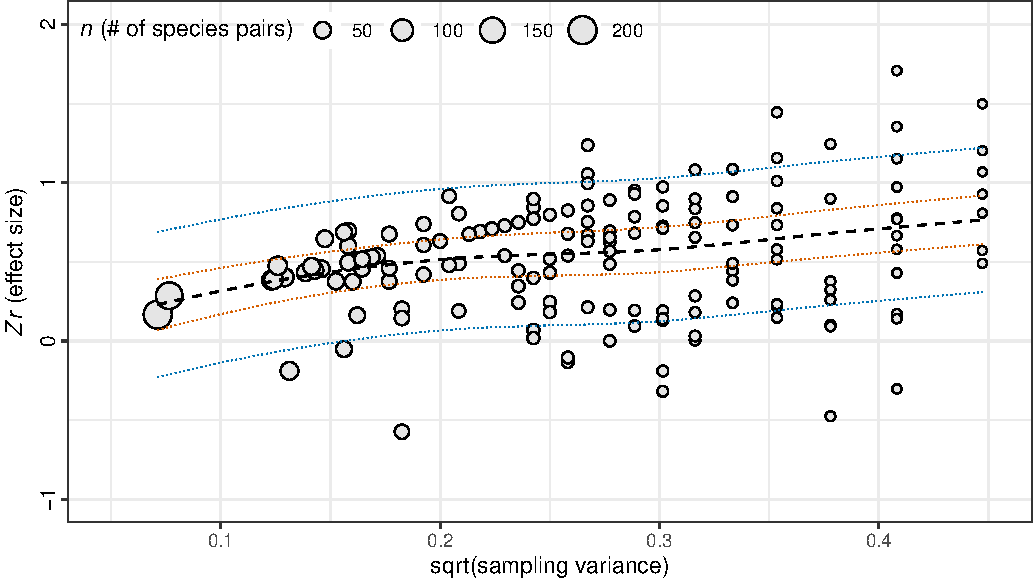
\includegraphics{Supporting_Information_files/figure-latex/unnamed-chunk-58-1.pdf}

\textbf{Supplementary Figure 8:} A bubble plot showing a predicted loess
line for the contentious variable \texttt{sqrt(VZr)} (given the values
of the other 3 variables in the model), with their 95\% confidence
regions (orange dotted lines) and 95\% prediction regions (blue dotted
lines) with observed effect sizes based on various sample sizes. Note
that the lines are not linear as these are based on multivariate
predictions of the data points.

\hypertarget{time-lag-bias}{%
\subsubsection{Time-lag bias}\label{time-lag-bias}}

We do not find any evidence of a time-lag effect (a decline in the
magnitude of the effect over time) in either the univariate or
multivariate models (\textbf{Supplementary Figure 9} and
\textbf{Supplementary Figure 10}).

\hypertarget{univariate-time-lag-bias}{%
\paragraph{Univariate time-lag bias}\label{univariate-time-lag-bias}}

\begin{Shaded}
\begin{Highlighting}[]
\CommentTok{# }
\NormalTok{time_lag_effect_uni <-}\StringTok{ }\KeywordTok{rma.mv}\NormalTok{(}\DataTypeTok{yi =}\NormalTok{ Zr, }\DataTypeTok{V =}\NormalTok{ VZr, }\DataTypeTok{mods =} \OperatorTok{~}\NormalTok{year, }\DataTypeTok{random =} \OperatorTok{~}\DecValTok{1} \OperatorTok{|}\StringTok{ }\NormalTok{authors, }
    \DataTypeTok{data =}\NormalTok{ dat)}
\end{Highlighting}
\end{Shaded}

\textbf{Supplementary Table 17:} Regression coefficients (Estimate),
95\% confidence intervals (CIs), variance components (V) and variance
explained, \emph{R}\textsuperscript{2}\textsubscript{{[}marginal{]}}
(R2) from the meta-regression with \texttt{year}.

\begin{Shaded}
\begin{Highlighting}[]
\CommentTok{# getting marginal R2}
\NormalTok{r2_time_lag_effect_uni <-}\StringTok{ }\KeywordTok{R2}\NormalTok{(time_lag_effect_uni)}

\CommentTok{# getting estimates: name does not work for slopes}
\NormalTok{res_time_lag_effect_uni <-}\StringTok{ }\KeywordTok{get_est}\NormalTok{(time_lag_effect_uni, }\DataTypeTok{mod =} \StringTok{"year"}\NormalTok{)}

\CommentTok{# creating a table}
\KeywordTok{tibble}\NormalTok{(}\StringTok{`}\DataTypeTok{Fixed effect}\StringTok{`}\NormalTok{ =}\StringTok{ }\KeywordTok{c}\NormalTok{(}\StringTok{"Intercept"}\NormalTok{, }\StringTok{"Year"}\NormalTok{), }\DataTypeTok{Estimate =} \KeywordTok{c}\NormalTok{(res_time_lag_effect_uni}\OperatorTok{$}\NormalTok{estimate), }
    \StringTok{`}\DataTypeTok{Lower CI [0.025]}\StringTok{`}\NormalTok{ =}\StringTok{ }\KeywordTok{c}\NormalTok{(res_time_lag_effect_uni}\OperatorTok{$}\NormalTok{lowerCL), }\StringTok{`}\DataTypeTok{Upper CI  [0.975]}\StringTok{`}\NormalTok{ =}\StringTok{ }\KeywordTok{c}\NormalTok{(res_time_lag_effect_uni}\OperatorTok{$}\NormalTok{upperCL), }
    \StringTok{`}\DataTypeTok{V[authors]}\StringTok{`}\NormalTok{ =}\StringTok{ }\KeywordTok{c}\NormalTok{(time_lag_effect_uni}\OperatorTok{$}\NormalTok{sigma2, }\OtherTok{NA}\NormalTok{), }\DataTypeTok{R2 =} \KeywordTok{c}\NormalTok{(r2_time_lag_effect_uni[}\DecValTok{1}\NormalTok{], }
        \OtherTok{NA}\NormalTok{)) }\OperatorTok\StringTok{ }\KeywordTok{kable}\NormalTok{(}\StringTok{"html"}\NormalTok{, }\DataTypeTok{digits =} \DecValTok{3}\NormalTok{) }\OperatorTok\StringTok{ }\KeywordTok{kable_styling}\NormalTok{(}\StringTok{"striped"}\NormalTok{, }\DataTypeTok{position =} \StringTok{"left"}\NormalTok{)}
\end{Highlighting}
\end{Shaded}

Fixed effect

Estimate

Lower CI {[}0.025{]}

Upper CI {[}0.975{]}

V{[}authors{]}

R2

Intercept

-4.848

-25.423

15.728

0.089

0.003

Year

0.003

-0.008

0.013

NA

NA

\begin{Shaded}
\begin{Highlighting}[]
\NormalTok{pred_time_lag_effect_uni <-}\StringTok{ }\KeywordTok{predict.rma}\NormalTok{(time_lag_effect_uni)}

\CommentTok{# plotting}

\NormalTok{fit_time_lag_effect <-}\StringTok{ }\NormalTok{dat }\OperatorTok\StringTok{ }\KeywordTok{mutate}\NormalTok{(}\DataTypeTok{ymin =}\NormalTok{ pred_time_lag_effect_uni}\OperatorTok{$}\NormalTok{ci.lb, }\DataTypeTok{ymax =}\NormalTok{ pred_time_lag_effect_uni}\OperatorTok{$}\NormalTok{ci.ub, }
    \DataTypeTok{ymin2 =}\NormalTok{ pred_time_lag_effect_uni}\OperatorTok{$}\NormalTok{cr.lb, }\DataTypeTok{ymax2 =}\NormalTok{ pred_time_lag_effect_uni}\OperatorTok{$}\NormalTok{cr.ub, }
    \DataTypeTok{pred =}\NormalTok{ pred_time_lag_effect_uni}\OperatorTok{$}\NormalTok{pred) }\OperatorTok\StringTok{ }\KeywordTok{ggplot}\NormalTok{(}\KeywordTok{aes}\NormalTok{(}\DataTypeTok{x =}\NormalTok{ year, }\DataTypeTok{y =}\NormalTok{ Zr, }\DataTypeTok{size =}\NormalTok{ (}\DecValTok{1}\OperatorTok{/}\NormalTok{VZr) }\OperatorTok{+}\StringTok{ }
\StringTok{    }\DecValTok{3}\NormalTok{)) }\OperatorTok{+}\StringTok{ }\KeywordTok{geom_point}\NormalTok{(}\DataTypeTok{shape =} \DecValTok{21}\NormalTok{, }\DataTypeTok{fill =} \StringTok{"grey90"}\NormalTok{) }\OperatorTok{+}\StringTok{ }\CommentTok{# geom_ribbon(aes(ymin = ymin, ymax = ymax), fill = '#0072B2') + # not quite sure}
\CommentTok{# why this does not work}
\KeywordTok{geom_smooth}\NormalTok{(}\KeywordTok{aes}\NormalTok{(}\DataTypeTok{y =}\NormalTok{ ymin2), }\DataTypeTok{method =} \StringTok{"loess"}\NormalTok{, }\DataTypeTok{se =} \OtherTok{FALSE}\NormalTok{, }\DataTypeTok{lty =} \StringTok{"dotted"}\NormalTok{, }\DataTypeTok{lwd =} \FloatTok{0.25}\NormalTok{, }
    \DataTypeTok{colour =} \StringTok{"#0072B2"}\NormalTok{) }\OperatorTok{+}\StringTok{ }\KeywordTok{geom_smooth}\NormalTok{(}\KeywordTok{aes}\NormalTok{(}\DataTypeTok{y =}\NormalTok{ ymax2), }\DataTypeTok{method =} \StringTok{"loess"}\NormalTok{, }\DataTypeTok{se =} \OtherTok{FALSE}\NormalTok{, }
    \DataTypeTok{lty =} \StringTok{"dotted"}\NormalTok{, }\DataTypeTok{lwd =} \FloatTok{0.25}\NormalTok{, }\DataTypeTok{colour =} \StringTok{"#0072B2"}\NormalTok{) }\OperatorTok{+}\StringTok{ }\KeywordTok{geom_smooth}\NormalTok{(}\KeywordTok{aes}\NormalTok{(}\DataTypeTok{y =}\NormalTok{ ymin), }
    \DataTypeTok{method =} \StringTok{"loess"}\NormalTok{, }\DataTypeTok{se =} \OtherTok{FALSE}\NormalTok{, }\DataTypeTok{lty =} \StringTok{"dotted"}\NormalTok{, }\DataTypeTok{lwd =} \FloatTok{0.25}\NormalTok{, }\DataTypeTok{colour =} \StringTok{"#D55E00"}\NormalTok{) }\OperatorTok{+}\StringTok{ }
\StringTok{    }\KeywordTok{geom_smooth}\NormalTok{(}\KeywordTok{aes}\NormalTok{(}\DataTypeTok{y =}\NormalTok{ ymax), }\DataTypeTok{method =} \StringTok{"loess"}\NormalTok{, }\DataTypeTok{se =} \OtherTok{FALSE}\NormalTok{, }\DataTypeTok{lty =} \StringTok{"dotted"}\NormalTok{, }\DataTypeTok{lwd =} \FloatTok{0.25}\NormalTok{, }
        \DataTypeTok{colour =} \StringTok{"#D55E00"}\NormalTok{) }\OperatorTok{+}\StringTok{ }\KeywordTok{geom_smooth}\NormalTok{(}\KeywordTok{aes}\NormalTok{(}\DataTypeTok{y =}\NormalTok{ pred), }\DataTypeTok{method =} \StringTok{"loess"}\NormalTok{, }\DataTypeTok{se =} \OtherTok{FALSE}\NormalTok{, }
    \DataTypeTok{lty =} \StringTok{"dashed"}\NormalTok{, }\DataTypeTok{lwd =} \FloatTok{0.5}\NormalTok{, }\DataTypeTok{colour =} \StringTok{"black"}\NormalTok{) }\OperatorTok{+}\StringTok{ }\KeywordTok{ylim}\NormalTok{(}\OperatorTok{-}\DecValTok{1}\NormalTok{, }\DecValTok{2}\NormalTok{) }\OperatorTok{+}\StringTok{ }\KeywordTok{xlim}\NormalTok{(}\DecValTok{1994}\NormalTok{, }\DecValTok{2019}\NormalTok{) }\OperatorTok{+}\StringTok{ }
\StringTok{    }\KeywordTok{scale_x_continuous}\NormalTok{(}\DataTypeTok{breaks =} \KeywordTok{c}\NormalTok{(}\DecValTok{1995}\NormalTok{, }\DecValTok{2000}\NormalTok{, }\DecValTok{2005}\NormalTok{, }\DecValTok{2010}\NormalTok{, }\DecValTok{2015}\NormalTok{, }\DecValTok{2020}\NormalTok{)) }\OperatorTok{+}\StringTok{ }\CommentTok{# geom_abline(intercept = mr_host_range_link_ratio$beta[[1]], slope =}
\CommentTok{# mr_host_range_link_ratio$beta[[2]], alpha = 0.7, linetype = 'dashed', size =}
\CommentTok{# 0.5) +}
\KeywordTok{labs}\NormalTok{(}\DataTypeTok{x =} \StringTok{"Year"}\NormalTok{, }\DataTypeTok{y =} \KeywordTok{expression}\NormalTok{(}\KeywordTok{paste}\NormalTok{(}\KeywordTok{italic}\NormalTok{(Zr), }\StringTok{" (effect size)"}\NormalTok{)), }\DataTypeTok{size =} \KeywordTok{expression}\NormalTok{(}\KeywordTok{paste}\NormalTok{(}\KeywordTok{italic}\NormalTok{(n), }
    \StringTok{" (# of species pairs)"}\NormalTok{))) }\OperatorTok{+}\StringTok{ }\KeywordTok{guides}\NormalTok{(}\DataTypeTok{fill =} \StringTok{"none"}\NormalTok{, }\DataTypeTok{colour =} \StringTok{"none"}\NormalTok{) }\OperatorTok{+}\StringTok{ }\CommentTok{# themses}
\KeywordTok{theme_bw}\NormalTok{() }\OperatorTok{+}\StringTok{ }\KeywordTok{theme}\NormalTok{(}\DataTypeTok{legend.position =} \KeywordTok{c}\NormalTok{(}\DecValTok{0}\NormalTok{, }\DecValTok{1}\NormalTok{), }\DataTypeTok{legend.justification =} \KeywordTok{c}\NormalTok{(}\DecValTok{0}\NormalTok{, }\DecValTok{1}\NormalTok{)) }\OperatorTok{+}\StringTok{ }\KeywordTok{theme}\NormalTok{(}\DataTypeTok{legend.direction =} \StringTok{"horizontal"}\NormalTok{) }\OperatorTok{+}\StringTok{ }
\StringTok{    }\CommentTok{# theme(legend.background = element_rect(fill = 'white', colour = 'black')) +}
\KeywordTok{theme}\NormalTok{(}\DataTypeTok{legend.background =} \KeywordTok{element_blank}\NormalTok{()) }\OperatorTok{+}\StringTok{ }\KeywordTok{theme}\NormalTok{(}\DataTypeTok{axis.text.y =} \KeywordTok{element_text}\NormalTok{(}\DataTypeTok{size =} \DecValTok{10}\NormalTok{, }
    \DataTypeTok{colour =} \StringTok{"black"}\NormalTok{, }\DataTypeTok{hjust =} \FloatTok{0.5}\NormalTok{, }\DataTypeTok{angle =} \DecValTok{90}\NormalTok{))}

\NormalTok{fit_time_lag_effect}
\end{Highlighting}
\end{Shaded}

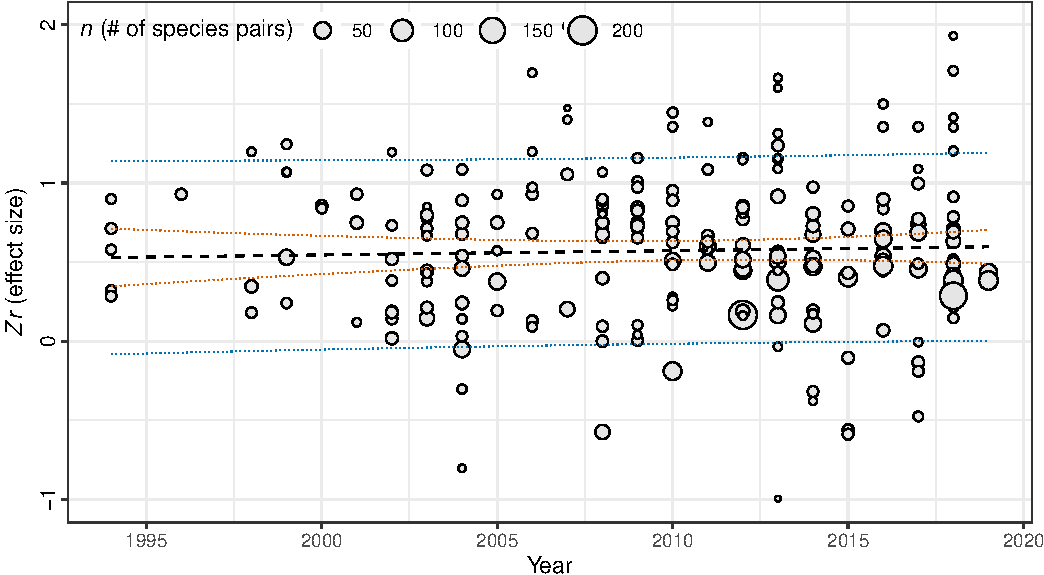
\includegraphics{Supporting_Information_files/figure-latex/unnamed-chunk-61-1.pdf}

\textbf{Supplementary Figure 9:} A bubble plot showing a predicted
regression line for the contentious variable \texttt{year}, indicating
95\% confidence regions (orange dotted lines) and 95\% prediction
regions (blue dotted lines), with observed effect sizes based on various
sample sizes.

\hypertarget{multivariate-time-lag-bias}{%
\paragraph{Multivariate time-lag
bias}\label{multivariate-time-lag-bias}}

\begin{Shaded}
\begin{Highlighting}[]
\CommentTok{# }
\NormalTok{time_lag_effect_mul <-}\StringTok{ }\KeywordTok{rma.mv}\NormalTok{(}\DataTypeTok{yi =}\NormalTok{ Zr, }\DataTypeTok{V =}\NormalTok{ VZr, }\DataTypeTok{mods =} \OperatorTok{~}\NormalTok{year }\OperatorTok{+}\StringTok{ }\NormalTok{mode_of_transmission_broad }\OperatorTok{+}\StringTok{ }
\StringTok{    }\NormalTok{host_tax_broad }\OperatorTok{+}\StringTok{ }\KeywordTok{log}\NormalTok{(host_range_link_ratio) }\OperatorTok{+}\StringTok{ }\NormalTok{symbiosis, }\DataTypeTok{random =} \OperatorTok{~}\DecValTok{1} \OperatorTok{|}\StringTok{ }\NormalTok{authors, }
    \DataTypeTok{data =}\NormalTok{ dat)}
\end{Highlighting}
\end{Shaded}

\textbf{Supplementary Table 18:} Regression coefficients (Estimate),
95\% confidence intervals (CIs), variance components (V) and variance
explained, \emph{R}\textsuperscript{2}\textsubscript{{[}marginal{]}}
(R2) from the meta-regression with \texttt{year}.

\begin{Shaded}
\begin{Highlighting}[]
\CommentTok{# getting marginal R2}
\NormalTok{r2_time_lag_effect_mul <-}\StringTok{ }\KeywordTok{R2}\NormalTok{(time_lag_effect_mul)}

\CommentTok{# creating a table}
\KeywordTok{tibble}\NormalTok{(}\StringTok{`}\DataTypeTok{Fixed effect}\StringTok{`}\NormalTok{ =}\StringTok{ }\KeywordTok{c}\NormalTok{(}\StringTok{"Intercept (both-Microbe-Mutulist)"}\NormalTok{, }\StringTok{"Year"}\NormalTok{, }\StringTok{"both-horizontal"}\NormalTok{, }
    \StringTok{"both-vertical"}\NormalTok{, }\StringTok{"Microbe-Plant"}\NormalTok{, }\StringTok{"Microbe-Invert"}\NormalTok{, }\StringTok{"Microbe-Vert"}\NormalTok{, }\StringTok{"host_range"}\NormalTok{, }
    \StringTok{"Mutulist-Parasite"}\NormalTok{), }\DataTypeTok{Estimate =} \KeywordTok{c}\NormalTok{(time_lag_effect_mul}\OperatorTok{$}\NormalTok{b), }\StringTok{`}\DataTypeTok{Lower CI [0.025]}\StringTok{`}\NormalTok{ =}\StringTok{ }\KeywordTok{c}\NormalTok{(time_lag_effect_mul}\OperatorTok{$}\NormalTok{ci.lb), }
    \StringTok{`}\DataTypeTok{Upper CI  [0.975]}\StringTok{`}\NormalTok{ =}\StringTok{ }\KeywordTok{c}\NormalTok{(time_lag_effect_mul}\OperatorTok{$}\NormalTok{ci.ub), }\StringTok{`}\DataTypeTok{V[authors]}\StringTok{`}\NormalTok{ =}\StringTok{ }\KeywordTok{c}\NormalTok{(time_lag_effect_mul}\OperatorTok{$}\NormalTok{sigma2, }
        \KeywordTok{rep}\NormalTok{(}\OtherTok{NA}\NormalTok{, }\DecValTok{8}\NormalTok{)), }\DataTypeTok{R2 =} \KeywordTok{c}\NormalTok{(r2_time_lag_effect_mul[}\DecValTok{1}\NormalTok{], }\KeywordTok{rep}\NormalTok{(}\OtherTok{NA}\NormalTok{, }\DecValTok{8}\NormalTok{))) }\OperatorTok\StringTok{ }\KeywordTok{kable}\NormalTok{(}\StringTok{"html"}\NormalTok{, }
    \DataTypeTok{digits =} \DecValTok{3}\NormalTok{) }\OperatorTok\StringTok{ }\KeywordTok{kable_styling}\NormalTok{(}\StringTok{"striped"}\NormalTok{, }\DataTypeTok{position =} \StringTok{"left"}\NormalTok{)}
\end{Highlighting}
\end{Shaded}

Fixed effect

Estimate

Lower CI {[}0.025{]}

Upper CI {[}0.975{]}

V{[}authors{]}

R2

Intercept (both-Microbe-Mutulist)

1.863

-18.349

22.075

0.073

0.234

Year

0.000

-0.011

0.010

NA

NA

both-horizontal

-0.075

-0.228

0.079

NA

NA

both-vertical

0.140

-0.135

0.416

NA

NA

Microbe-Plant

-0.455

-0.748

-0.163

NA

NA

Microbe-Invert

-0.330

-0.619

-0.041

NA

NA

Microbe-Vert

-0.276

-0.552

0.000

NA

NA

host\_range

0.095

-0.073

0.262

NA

NA

Mutulist-Parasite

-0.069

-0.260

0.123

NA

NA

\begin{Shaded}
\begin{Highlighting}[]
\NormalTok{pred_time_lag_effect_mul <-}\StringTok{ }\KeywordTok{predict.rma}\NormalTok{(time_lag_effect_mul)}

\CommentTok{# plotting}
\NormalTok{fit_time_lag_effect_mul <-}\StringTok{ }\NormalTok{dat }\OperatorTok\StringTok{ }\KeywordTok{filter}\NormalTok{(}\OperatorTok{!}\KeywordTok{is.na}\NormalTok{(mode_of_transmission_broad) }\OperatorTok{&}\StringTok{ }\OperatorTok{!}\KeywordTok{is.na}\NormalTok{(host_tax_broad) }\OperatorTok{&}\StringTok{ }
\StringTok{    }\OperatorTok{!}\KeywordTok{is.na}\NormalTok{(symbiosis) }\OperatorTok{&}\StringTok{ }\OperatorTok{!}\KeywordTok{is.na}\NormalTok{(host_range_link_ratio)) }\OperatorTok\StringTok{ }\KeywordTok{mutate}\NormalTok{(}\DataTypeTok{ymin =}\NormalTok{ pred_time_lag_effect_mul}\OperatorTok{$}\NormalTok{ci.lb, }
    \DataTypeTok{ymax =}\NormalTok{ pred_time_lag_effect_mul}\OperatorTok{$}\NormalTok{ci.ub, }\DataTypeTok{ymin2 =}\NormalTok{ pred_time_lag_effect_mul}\OperatorTok{$}\NormalTok{cr.lb, }
    \DataTypeTok{ymax2 =}\NormalTok{ pred_time_lag_effect_mul}\OperatorTok{$}\NormalTok{cr.ub, }\DataTypeTok{pred =}\NormalTok{ pred_time_lag_effect_mul}\OperatorTok{$}\NormalTok{pred) }\OperatorTok\StringTok{ }
\StringTok{    }\KeywordTok{ggplot}\NormalTok{(}\KeywordTok{aes}\NormalTok{(}\DataTypeTok{x =}\NormalTok{ year, }\DataTypeTok{y =}\NormalTok{ Zr, }\DataTypeTok{size =}\NormalTok{ (}\DecValTok{1}\OperatorTok{/}\NormalTok{VZr) }\OperatorTok{+}\StringTok{ }\DecValTok{3}\NormalTok{)) }\OperatorTok{+}\StringTok{ }\KeywordTok{geom_point}\NormalTok{(}\DataTypeTok{shape =} \DecValTok{21}\NormalTok{, }\DataTypeTok{fill =} \StringTok{"grey90"}\NormalTok{) }\OperatorTok{+}\StringTok{ }
\StringTok{    }\CommentTok{# geom_ribbon(aes(ymin = ymin, ymax = ymax), fill = '#0072B2') + # not quite sure}
\CommentTok{# why this does not work}
\KeywordTok{geom_smooth}\NormalTok{(}\KeywordTok{aes}\NormalTok{(}\DataTypeTok{y =}\NormalTok{ ymin2), }\DataTypeTok{method =} \StringTok{"loess"}\NormalTok{, }\DataTypeTok{se =} \OtherTok{FALSE}\NormalTok{, }\DataTypeTok{lty =} \StringTok{"dotted"}\NormalTok{, }\DataTypeTok{lwd =} \FloatTok{0.25}\NormalTok{, }
    \DataTypeTok{colour =} \StringTok{"#0072B2"}\NormalTok{) }\OperatorTok{+}\StringTok{ }\KeywordTok{geom_smooth}\NormalTok{(}\KeywordTok{aes}\NormalTok{(}\DataTypeTok{y =}\NormalTok{ ymax2), }\DataTypeTok{method =} \StringTok{"loess"}\NormalTok{, }\DataTypeTok{se =} \OtherTok{FALSE}\NormalTok{, }
    \DataTypeTok{lty =} \StringTok{"dotted"}\NormalTok{, }\DataTypeTok{lwd =} \FloatTok{0.25}\NormalTok{, }\DataTypeTok{colour =} \StringTok{"#0072B2"}\NormalTok{) }\OperatorTok{+}\StringTok{ }\KeywordTok{geom_smooth}\NormalTok{(}\KeywordTok{aes}\NormalTok{(}\DataTypeTok{y =}\NormalTok{ ymin), }
    \DataTypeTok{method =} \StringTok{"loess"}\NormalTok{, }\DataTypeTok{se =} \OtherTok{FALSE}\NormalTok{, }\DataTypeTok{lty =} \StringTok{"dotted"}\NormalTok{, }\DataTypeTok{lwd =} \FloatTok{0.25}\NormalTok{, }\DataTypeTok{colour =} \StringTok{"#D55E00"}\NormalTok{) }\OperatorTok{+}\StringTok{ }
\StringTok{    }\KeywordTok{geom_smooth}\NormalTok{(}\KeywordTok{aes}\NormalTok{(}\DataTypeTok{y =}\NormalTok{ ymax), }\DataTypeTok{method =} \StringTok{"loess"}\NormalTok{, }\DataTypeTok{se =} \OtherTok{FALSE}\NormalTok{, }\DataTypeTok{lty =} \StringTok{"dotted"}\NormalTok{, }\DataTypeTok{lwd =} \FloatTok{0.25}\NormalTok{, }
        \DataTypeTok{colour =} \StringTok{"#D55E00"}\NormalTok{) }\OperatorTok{+}\StringTok{ }\KeywordTok{geom_smooth}\NormalTok{(}\KeywordTok{aes}\NormalTok{(}\DataTypeTok{y =}\NormalTok{ pred), }\DataTypeTok{method =} \StringTok{"loess"}\NormalTok{, }\DataTypeTok{se =} \OtherTok{FALSE}\NormalTok{, }
    \DataTypeTok{lty =} \StringTok{"dashed"}\NormalTok{, }\DataTypeTok{lwd =} \FloatTok{0.5}\NormalTok{, }\DataTypeTok{colour =} \StringTok{"black"}\NormalTok{) }\OperatorTok{+}\StringTok{ }\KeywordTok{ylim}\NormalTok{(}\OperatorTok{-}\DecValTok{1}\NormalTok{, }\DecValTok{2}\NormalTok{) }\OperatorTok{+}\StringTok{ }\KeywordTok{xlim}\NormalTok{(}\DecValTok{1994}\NormalTok{, }\DecValTok{2019}\NormalTok{) }\OperatorTok{+}\StringTok{ }
\StringTok{    }\KeywordTok{scale_x_continuous}\NormalTok{(}\DataTypeTok{breaks =} \KeywordTok{c}\NormalTok{(}\DecValTok{1995}\NormalTok{, }\DecValTok{2000}\NormalTok{, }\DecValTok{2005}\NormalTok{, }\DecValTok{2010}\NormalTok{, }\DecValTok{2015}\NormalTok{, }\DecValTok{2020}\NormalTok{)) }\OperatorTok{+}\StringTok{ }\CommentTok{# geom_abline(intercept = mr_host_range_link_ratio$beta[[1]], slope =}
\CommentTok{# mr_host_range_link_ratio$beta[[2]], alpha = 0.7, linetype = 'dashed', size =}
\CommentTok{# 0.5) +}
\KeywordTok{labs}\NormalTok{(}\DataTypeTok{x =} \StringTok{"Year"}\NormalTok{, }\DataTypeTok{y =} \KeywordTok{expression}\NormalTok{(}\KeywordTok{paste}\NormalTok{(}\KeywordTok{italic}\NormalTok{(Zr), }\StringTok{" (effect size)"}\NormalTok{)), }\DataTypeTok{size =} \KeywordTok{expression}\NormalTok{(}\KeywordTok{paste}\NormalTok{(}\KeywordTok{italic}\NormalTok{(n), }
    \StringTok{" (# of species pairs)"}\NormalTok{))) }\OperatorTok{+}\StringTok{ }\KeywordTok{guides}\NormalTok{(}\DataTypeTok{fill =} \StringTok{"none"}\NormalTok{, }\DataTypeTok{colour =} \StringTok{"none"}\NormalTok{) }\OperatorTok{+}\StringTok{ }\CommentTok{# themses}
\KeywordTok{theme_bw}\NormalTok{() }\OperatorTok{+}\StringTok{ }\KeywordTok{theme}\NormalTok{(}\DataTypeTok{legend.position =} \KeywordTok{c}\NormalTok{(}\DecValTok{0}\NormalTok{, }\DecValTok{1}\NormalTok{), }\DataTypeTok{legend.justification =} \KeywordTok{c}\NormalTok{(}\DecValTok{0}\NormalTok{, }\DecValTok{1}\NormalTok{)) }\OperatorTok{+}\StringTok{ }\KeywordTok{theme}\NormalTok{(}\DataTypeTok{legend.direction =} \StringTok{"horizontal"}\NormalTok{) }\OperatorTok{+}\StringTok{ }
\StringTok{    }\CommentTok{# theme(legend.background = element_rect(fill = 'white', colour = 'black')) +}
\KeywordTok{theme}\NormalTok{(}\DataTypeTok{legend.background =} \KeywordTok{element_blank}\NormalTok{()) }\OperatorTok{+}\StringTok{ }\KeywordTok{theme}\NormalTok{(}\DataTypeTok{axis.text.y =} \KeywordTok{element_text}\NormalTok{(}\DataTypeTok{size =} \DecValTok{10}\NormalTok{, }
    \DataTypeTok{colour =} \StringTok{"black"}\NormalTok{, }\DataTypeTok{hjust =} \FloatTok{0.5}\NormalTok{, }\DataTypeTok{angle =} \DecValTok{90}\NormalTok{))}

\NormalTok{fit_time_lag_effect_mul}
\end{Highlighting}
\end{Shaded}

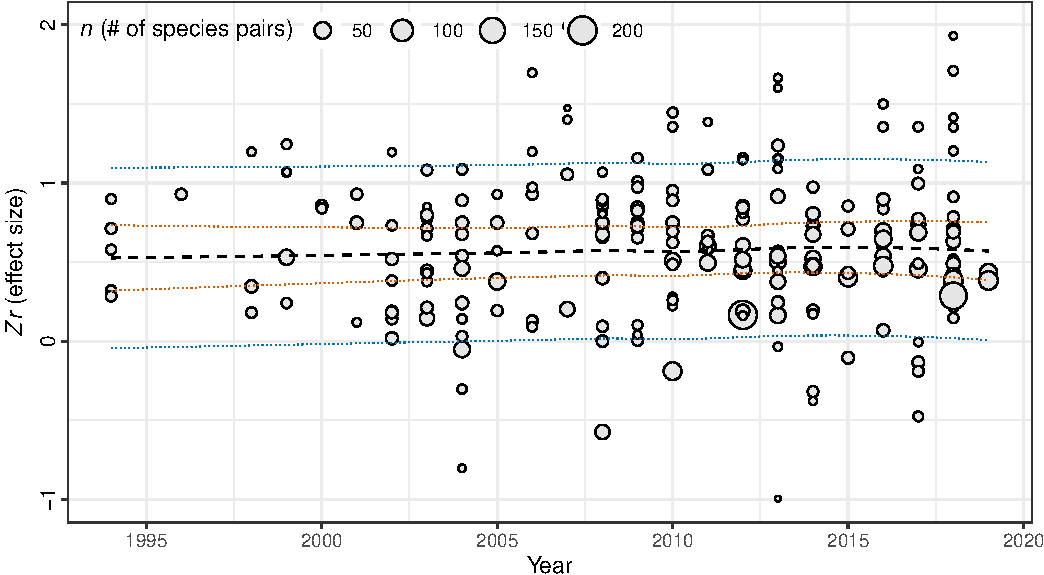
\includegraphics{Supporting_Information_files/figure-latex/unnamed-chunk-64-1.pdf}

\textbf{Supplementary Figure 10:} A bubble plot showing a predicted
loess line for the contentious variable \texttt{year} (given the values
of the other 3 variables in the model), indicating 95\% confidence
regions (orange dotted lines) and 95\% prediction regions (blue dotted
lines) with observed effect sizes based on various sample sizes. Note
that the lines are not linear as these are based on multivariate
predictions of the data points.

\hypertarget{sensitivity-analysis}{%
\subsection{Sensitivity Analysis}\label{sensitivity-analysis}}

The funnel plots above identified the issue of upper bounds for the
effect size given a sample size (an upper limit of a \emph{p} value
given the number of randomizations). This boundary would influence our
estimates of mean effect sizes and contrasts (i.e., comparing two
groups), often making our overall conclusions too conservative. To
demonstrate this, we conducted two analyses to show: 1) the number of
randomizations (\texttt{log(no\_randomizations)}) do not differ between
categories in the 3 important categorical moderators
(\texttt{mode\_of\_transmission\_broad}, \texttt{host\_tax\_broad}, \&
\texttt{symbiosis}), and, 2) categories with high effect sizes would
include ``bounded'' effect sizes (i.e., from \emph{p} = 0.01, 0.001, or
0.0001; \texttt{limit\_reached}) in the 3 moderators.

\hypertarget{sensitivity-test-1-the-number-of-randomizations}{%
\subsubsection{Sensitivity test 1: the number of
randomizations}\label{sensitivity-test-1-the-number-of-randomizations}}

Below, we showed that none of categorizes have significantly different
numbers of randomizations in all \texttt{mode\_of\_transmission\_broad},
\texttt{host\_tax\_broad}, \& \texttt{symbiosis}.

\hypertarget{the-type-of-symbiosis-parasitism-vs.-mutualism-1}{%
\paragraph{The type of symbiosis: parasitism
vs.~mutualism}\label{the-type-of-symbiosis-parasitism-vs.-mutualism-1}}

\begin{Shaded}
\begin{Highlighting}[]
\CommentTok{# 233 --- Yes = 74 (0.3175966%); No = 159}

\CommentTok{# symbiosis multiple intercepts}
\NormalTok{sa_random_symbiosis1 <-}\StringTok{ }\KeywordTok{lmer}\NormalTok{(}\KeywordTok{log}\NormalTok{(no_randomizations) }\OperatorTok{~}\StringTok{ }\NormalTok{symbiosis }\OperatorTok{-}\StringTok{ }\DecValTok{1} \OperatorTok{+}\StringTok{ }\NormalTok{(}\DecValTok{1} \OperatorTok{|}\StringTok{ }\NormalTok{authors), }
    \DataTypeTok{data =}\NormalTok{ dat)}
\CommentTok{# contrast}
\NormalTok{sa_random_symbiosis2 <-}\StringTok{ }\KeywordTok{lmer}\NormalTok{(}\KeywordTok{log}\NormalTok{(no_randomizations) }\OperatorTok{~}\StringTok{ }\NormalTok{symbiosis }\OperatorTok{+}\StringTok{ }\NormalTok{(}\DecValTok{1} \OperatorTok{|}\StringTok{ }\NormalTok{authors), }
    \DataTypeTok{data =}\NormalTok{ dat)}
\end{Highlighting}
\end{Shaded}

\textbf{Supplementary Table 19:} Regression coefficients (Estimate),
95\% confidence intervals (CIs), variance components (V) and variance
explained, \emph{R}\textsuperscript{2}\textsubscript{{[}marginal{]}}
(R2), from the regression with \texttt{symbiosis} on
\texttt{log(no\_randomizations)}.

\begin{Shaded}
\begin{Highlighting}[]
\CommentTok{# getting marginal R2}
\NormalTok{r2_sa_random_symbiosis <-}\StringTok{ }\KeywordTok{r2_nakagawa}\NormalTok{(sa_random_symbiosis1)}

\CommentTok{# getting estimates}

\NormalTok{res_sa_random_symbiosis <-}\StringTok{ }\KeywordTok{tibble}\NormalTok{(}\DataTypeTok{estiamte =} \KeywordTok{c}\NormalTok{(}\KeywordTok{fixef}\NormalTok{(sa_random_symbiosis1), }\KeywordTok{fixef}\NormalTok{(sa_random_symbiosis2)[}\DecValTok{2}\NormalTok{]))}

\NormalTok{ci_sa_random_symbiosis1 <-}\StringTok{ }\KeywordTok{confint}\NormalTok{(sa_random_symbiosis1)}
\NormalTok{ci_sa_random_symbiosis2 <-}\StringTok{ }\KeywordTok{confint}\NormalTok{(sa_random_symbiosis2)}
\NormalTok{res_sa_random_symbiosis }\OperatorTok\StringTok{ }\KeywordTok{mutate}\NormalTok{(}\DataTypeTok{lowerCL =} \KeywordTok{c}\NormalTok{(ci_sa_random_symbiosis1[}\DecValTok{3}\OperatorTok{:}\DecValTok{4}\NormalTok{, }\DecValTok{1}\NormalTok{], }
\NormalTok{    ci_sa_random_symbiosis2[}\DecValTok{4}\NormalTok{, }\DecValTok{1}\NormalTok{]))}
\NormalTok{res_sa_random_symbiosis }\OperatorTok\StringTok{ }\KeywordTok{mutate}\NormalTok{(}\DataTypeTok{upperCL =} \KeywordTok{c}\NormalTok{(ci_sa_random_symbiosis1[}\DecValTok{3}\OperatorTok{:}\DecValTok{4}\NormalTok{, }\DecValTok{2}\NormalTok{], }
\NormalTok{    ci_sa_random_symbiosis2[}\DecValTok{4}\NormalTok{, }\DecValTok{2}\NormalTok{]))}

\CommentTok{# creating a table}
\KeywordTok{tibble}\NormalTok{(}\StringTok{`}\DataTypeTok{Fixed effect}\StringTok{`}\NormalTok{ =}\StringTok{ }\KeywordTok{c}\NormalTok{(}\KeywordTok{as.character}\NormalTok{(res_symbiosis1}\OperatorTok{$}\NormalTok{name), }\KeywordTok{cont_gen}\NormalTok{(res_symbiosis1}\OperatorTok{$}\NormalTok{name)), }
    \DataTypeTok{Estimate =}\NormalTok{ res_sa_random_symbiosis}\OperatorTok{$}\NormalTok{estiamte, }\StringTok{`}\DataTypeTok{Lower CI [0.025]}\StringTok{`}\NormalTok{ =}\StringTok{ }\NormalTok{res_sa_random_symbiosis}\OperatorTok{$}\NormalTok{lowerCL, }
    \StringTok{`}\DataTypeTok{Upper CI  [0.975]}\StringTok{`}\NormalTok{ =}\StringTok{ }\NormalTok{res_sa_random_symbiosis}\OperatorTok{$}\NormalTok{upperCL, }\StringTok{`}\DataTypeTok{V[authors]}\StringTok{`}\NormalTok{ =}\StringTok{ }\KeywordTok{c}\NormalTok{(}\KeywordTok{attr}\NormalTok{(}\KeywordTok{VarCorr}\NormalTok{(sa_random_symbiosis1)}\OperatorTok{$}\NormalTok{author, }
        \StringTok{"stddev"}\NormalTok{)}\OperatorTok{^}\DecValTok{2}\NormalTok{, }\KeywordTok{rep}\NormalTok{(}\OtherTok{NA}\NormalTok{, }\DecValTok{2}\NormalTok{)), }\StringTok{`}\DataTypeTok{V[residuals]}\StringTok{`}\NormalTok{ =}\StringTok{ }\KeywordTok{c}\NormalTok{(}\KeywordTok{attr}\NormalTok{(}\KeywordTok{VarCorr}\NormalTok{(sa_random_symbiosis1), }
        \StringTok{"sc"}\NormalTok{)}\OperatorTok{^}\DecValTok{2}\NormalTok{, }\KeywordTok{rep}\NormalTok{(}\OtherTok{NA}\NormalTok{, }\DecValTok{2}\NormalTok{)), }\DataTypeTok{R2 =} \KeywordTok{c}\NormalTok{(r2_sa_random_symbiosis}\OperatorTok{$}\NormalTok{R2_marginal, }\KeywordTok{rep}\NormalTok{(}\OtherTok{NA}\NormalTok{, }
        \DecValTok{2}\NormalTok{))) }\OperatorTok\StringTok{ }\KeywordTok{kable}\NormalTok{(}\StringTok{"html"}\NormalTok{, }\DataTypeTok{digits =} \DecValTok{3}\NormalTok{) }\OperatorTok\StringTok{ }\KeywordTok{kable_styling}\NormalTok{(}\StringTok{"striped"}\NormalTok{, }\DataTypeTok{position =} \StringTok{"left"}\NormalTok{)}
\end{Highlighting}
\end{Shaded}

Fixed effect

Estimate

Lower CI {[}0.025{]}

Upper CI {[}0.975{]}

V{[}authors{]}

V{[}residuals{]}

R2

Mutualist

7.696

7.286

8.106

2.931

0.352

0.004

Parasite

7.619

7.314

7.924

NA

NA

NA

Mutualist-Parasite

-0.077

-0.544

0.389

NA

NA

NA

\hypertarget{the-effect-of-host-taxa-1}{%
\paragraph{The effect of host taxa}\label{the-effect-of-host-taxa-1}}

\begin{Shaded}
\begin{Highlighting}[]
\CommentTok{# host_tax_broad mutiple intercepts}
\NormalTok{sa_random_host_tax_broad1 <-}\StringTok{ }\KeywordTok{lmer}\NormalTok{(}\KeywordTok{log}\NormalTok{(no_randomizations) }\OperatorTok{~}\StringTok{ }\NormalTok{host_tax_broad }\OperatorTok{-}\StringTok{ }\DecValTok{1} \OperatorTok{+}\StringTok{ }\NormalTok{(}\DecValTok{1} \OperatorTok{|}\StringTok{ }
\StringTok{    }\NormalTok{authors), }\DataTypeTok{data =}\NormalTok{ dat)}
\CommentTok{# contrast 1}
\NormalTok{sa_random_host_tax_broad2 <-}\StringTok{ }\KeywordTok{lmer}\NormalTok{(}\KeywordTok{log}\NormalTok{(no_randomizations) }\OperatorTok{~}\StringTok{ }\NormalTok{host_tax_broad }\OperatorTok{+}\StringTok{ }\NormalTok{(}\DecValTok{1} \OperatorTok{|}\StringTok{ }
\StringTok{    }\NormalTok{authors), }\DataTypeTok{data =}\NormalTok{ dat)}
\CommentTok{# contrast 2}
\NormalTok{sa_random_host_tax_broad3 <-}\StringTok{ }\KeywordTok{lmer}\NormalTok{(}\KeywordTok{log}\NormalTok{(no_randomizations) }\OperatorTok{~}\StringTok{ }\KeywordTok{relevel}\NormalTok{(host_tax_broad, }
    \DataTypeTok{ref =} \StringTok{"Plant"}\NormalTok{) }\OperatorTok{+}\StringTok{ }\NormalTok{(}\DecValTok{1} \OperatorTok{|}\StringTok{ }\NormalTok{authors), }\DataTypeTok{data =}\NormalTok{ dat)}

\CommentTok{# contrast 3}
\NormalTok{sa_random_host_tax_broad4 <-}\StringTok{ }\KeywordTok{lmer}\NormalTok{(}\KeywordTok{log}\NormalTok{(no_randomizations) }\OperatorTok{~}\StringTok{ }\KeywordTok{relevel}\NormalTok{(host_tax_broad, }
    \DataTypeTok{ref =} \StringTok{"Invert"}\NormalTok{) }\OperatorTok{+}\StringTok{ }\NormalTok{(}\DecValTok{1} \OperatorTok{|}\StringTok{ }\NormalTok{authors), }\DataTypeTok{data =}\NormalTok{ dat)}
\end{Highlighting}
\end{Shaded}

\textbf{Supplementary Table 20:} Regression coefficients (estimate),
95\% confidence intervals (CIs), variance components (V) and variance
explained, \emph{R}\textsuperscript{2}\textsubscript{{[}marginal{]}}
(R2) from the regression with \texttt{host\_tax\_broad} on
\texttt{log(no\_randomizations)}.

\begin{Shaded}
\begin{Highlighting}[]
\CommentTok{# getting marginal R2}
\NormalTok{r2_sa_random_host_tax_broad <-}\StringTok{ }\KeywordTok{r2_nakagawa}\NormalTok{(sa_random_host_tax_broad1)}

\CommentTok{# getting estimates}
\NormalTok{res_sa_random_host_tax_broad <-}\StringTok{ }\KeywordTok{tibble}\NormalTok{(}\DataTypeTok{estiamte =} \KeywordTok{c}\NormalTok{(}\KeywordTok{fixef}\NormalTok{(sa_random_host_tax_broad1), }
                                                    \KeywordTok{fixef}\NormalTok{(sa_random_host_tax_broad2)[}\DecValTok{2}\OperatorTok{:}\DecValTok{4}\NormalTok{],}
                                                    \KeywordTok{fixef}\NormalTok{(sa_random_host_tax_broad3)[}\DecValTok{3}\OperatorTok{:}\DecValTok{4}\NormalTok{],}
                                                    \KeywordTok{fixef}\NormalTok{(sa_random_host_tax_broad4)[}\DecValTok{4}\NormalTok{])) }
  
\NormalTok{ci_sa_random_host_tax_broad1<-}\KeywordTok{confint}\NormalTok{(sa_random_host_tax_broad1)}
\NormalTok{ci_sa_random_host_tax_broad2<-}\KeywordTok{confint}\NormalTok{(sa_random_host_tax_broad2)}
\NormalTok{ci_sa_random_host_tax_broad3<-}\KeywordTok{confint}\NormalTok{(sa_random_host_tax_broad3)}
\NormalTok{ci_sa_random_host_tax_broad4<-}\KeywordTok{confint}\NormalTok{(sa_random_host_tax_broad4)}
\NormalTok{res_sa_random_host_tax_broad }\OperatorTok\StringTok{ }\KeywordTok{mutate}\NormalTok{(}\DataTypeTok{lowerCL =} \KeywordTok{c}\NormalTok{(ci_sa_random_host_tax_broad1[}\DecValTok{3}\OperatorTok{:}\DecValTok{6}\NormalTok{,}\DecValTok{1}\NormalTok{], }
\NormalTok{                                                ci_sa_random_host_tax_broad2[}\DecValTok{4}\OperatorTok{:}\DecValTok{6}\NormalTok{,}\DecValTok{1}\NormalTok{],}
\NormalTok{                                                ci_sa_random_host_tax_broad3[}\DecValTok{5}\OperatorTok{:}\DecValTok{6}\NormalTok{,}\DecValTok{1}\NormalTok{],}
\NormalTok{                                                ci_sa_random_host_tax_broad4[}\DecValTok{6}\NormalTok{,}\DecValTok{1}\NormalTok{]))}
\NormalTok{res_sa_random_host_tax_broad }\OperatorTok\StringTok{ }\KeywordTok{mutate}\NormalTok{(}\DataTypeTok{upperCL =} \KeywordTok{c}\NormalTok{(ci_sa_random_host_tax_broad1[}\DecValTok{3}\OperatorTok{:}\DecValTok{6}\NormalTok{,}\DecValTok{2}\NormalTok{], }
\NormalTok{                                                ci_sa_random_host_tax_broad2[}\DecValTok{4}\OperatorTok{:}\DecValTok{6}\NormalTok{,}\DecValTok{2}\NormalTok{],}
\NormalTok{                                                ci_sa_random_host_tax_broad3[}\DecValTok{5}\OperatorTok{:}\DecValTok{6}\NormalTok{,}\DecValTok{2}\NormalTok{],}
\NormalTok{                                                ci_sa_random_host_tax_broad4[}\DecValTok{6}\NormalTok{,}\DecValTok{2}\NormalTok{]))}
\CommentTok{# creating a table}
\KeywordTok{tibble}\NormalTok{(}
  \StringTok{`}\DataTypeTok{Fixed effect}\StringTok{`}\NormalTok{ =}\StringTok{  }\KeywordTok{c}\NormalTok{(}\KeywordTok{as.character}\NormalTok{(res_symbiont_tax_broad1}\OperatorTok{$}\NormalTok{name), }\KeywordTok{cont_gen}\NormalTok{(res_symbiont_tax_broad1}\OperatorTok{$}\NormalTok{name)), }\CommentTok{# done}
  \DataTypeTok{Estimate =}\NormalTok{ res_sa_random_host_tax_broad}\OperatorTok{$}\NormalTok{estiamte,}
  \StringTok{`}\DataTypeTok{Lower CI [0.025]}\StringTok{`}\NormalTok{ =}\StringTok{ }\NormalTok{res_sa_random_host_tax_broad}\OperatorTok{$}\NormalTok{lowerCL,}
  \StringTok{`}\DataTypeTok{Upper CI  [0.975]}\StringTok{`}\NormalTok{ =}\StringTok{ }\NormalTok{res_sa_random_host_tax_broad}\OperatorTok{$}\NormalTok{upperCL,}
  \StringTok{`}\DataTypeTok{V[authors]}\StringTok{`}\NormalTok{ =}\StringTok{ }\KeywordTok{c}\NormalTok{(}\KeywordTok{attr}\NormalTok{(}\KeywordTok{VarCorr}\NormalTok{(sa_random_host_tax_broad1)}\OperatorTok{$}\NormalTok{author,}\StringTok{"stddev"}\NormalTok{)}\OperatorTok{^}\DecValTok{2}\NormalTok{,  }\KeywordTok{rep}\NormalTok{(}\OtherTok{NA}\NormalTok{, }\DecValTok{9}\NormalTok{)),}
  \StringTok{`}\DataTypeTok{V[residuals]}\StringTok{`}\NormalTok{ =}\KeywordTok{c}\NormalTok{(}\KeywordTok{attr}\NormalTok{(}\KeywordTok{VarCorr}\NormalTok{(sa_random_host_tax_broad1),}\StringTok{"sc"}\NormalTok{)}\OperatorTok{^}\DecValTok{2}\NormalTok{, }\KeywordTok{rep}\NormalTok{(}\OtherTok{NA}\NormalTok{, }\DecValTok{9}\NormalTok{)),}
  \StringTok{`}\DataTypeTok{R2}\StringTok{`}\NormalTok{ =}\StringTok{ }\KeywordTok{c}\NormalTok{(r2_sa_random_host_tax_broad}\OperatorTok{$}\NormalTok{R2_marginal, }\KeywordTok{rep}\NormalTok{(}\OtherTok{NA}\NormalTok{, }\DecValTok{9}\NormalTok{))) }\OperatorTok\StringTok{ }\KeywordTok{kable}\NormalTok{(}\StringTok{"html"}\NormalTok{, }\DataTypeTok{digits =} \DecValTok{3}\NormalTok{) }\OperatorTok
\StringTok{  }\KeywordTok{kable_styling}\NormalTok{(}\StringTok{"striped"}\NormalTok{, }\DataTypeTok{position =} \StringTok{"left"}\NormalTok{) }
\end{Highlighting}
\end{Shaded}

Fixed effect

Estimate

Lower CI {[}0.025{]}

Upper CI {[}0.975{]}

V{[}authors{]}

V{[}residuals{]}

R2

Microbe

8.223

7.279

9.168

2.937

0.35

0.071

Plant

7.466

6.856

8.076

NA

NA

NA

Invert

7.650

7.167

8.134

NA

NA

NA

Vert

7.634

7.265

8.003

NA

NA

NA

Microbe-Plant

-0.757

-1.882

0.367

NA

NA

NA

Microbe-Invert

-0.573

-1.634

0.488

NA

NA

NA

Microbe-Vert

-0.589

-1.603

0.425

NA

NA

NA

Plant-Invert

0.184

-0.594

0.962

NA

NA

NA

Plant-Vert

0.168

-0.545

0.881

NA

NA

NA

Invert-Vert

-0.016

-0.599

0.566

NA

NA

NA

\hypertarget{the-effect-of-the-model-of-transmission}{%
\paragraph{The effect of the model of
transmission}\label{the-effect-of-the-model-of-transmission}}

\begin{Shaded}
\begin{Highlighting}[]
\CommentTok{# mode_of_transmission_broad}

\NormalTok{sa_random_mode_of_transmission_broad1 <-}\StringTok{ }\KeywordTok{lmer}\NormalTok{(}\KeywordTok{log}\NormalTok{(no_randomizations) }\OperatorTok{~}\StringTok{ }\NormalTok{mode_of_transmission_broad }\OperatorTok{-}\StringTok{ }
\StringTok{    }\DecValTok{1} \OperatorTok{+}\StringTok{ }\NormalTok{(}\DecValTok{1} \OperatorTok{|}\StringTok{ }\NormalTok{authors), }\DataTypeTok{data =}\NormalTok{ dat)}


\CommentTok{# contrast 1}
\NormalTok{sa_random_mode_of_transmission_broad2 <-}\StringTok{ }\KeywordTok{lmer}\NormalTok{(}\KeywordTok{log}\NormalTok{(no_randomizations) }\OperatorTok{~}\StringTok{ }\NormalTok{mode_of_transmission_broad }\OperatorTok{+}\StringTok{ }
\StringTok{    }\NormalTok{(}\DecValTok{1} \OperatorTok{|}\StringTok{ }\NormalTok{authors), }\DataTypeTok{data =}\NormalTok{ dat)}

\CommentTok{# contrast 2}
\NormalTok{sa_random_mode_of_transmission_broad3 <-}\StringTok{ }\KeywordTok{lmer}\NormalTok{(}\KeywordTok{log}\NormalTok{(no_randomizations) }\OperatorTok{~}\StringTok{ }\KeywordTok{relevel}\NormalTok{(mode_of_transmission_broad, }
    \DataTypeTok{ref =} \StringTok{"vertical"}\NormalTok{) }\OperatorTok{+}\StringTok{ }\NormalTok{(}\DecValTok{1} \OperatorTok{|}\StringTok{ }\NormalTok{authors), }\DataTypeTok{data =}\NormalTok{ dat)}
\end{Highlighting}
\end{Shaded}

\textbf{Supplementary Table 21:} Regression coefficients (estimate),
95\% confidence intervals (CIs), variance components (V) and variance
explained, \emph{R}\textsuperscript{2}\textsubscript{{[}marginal{]}}
(R2) from the regression with \texttt{mode\_of\_transmission\_broad} on
\texttt{log(no\_randomizations)}.

\begin{Shaded}
\begin{Highlighting}[]
\CommentTok{# getting marginal R2}
\NormalTok{r2_sa_random_mode_of_transmission_broad <-}\StringTok{ }\KeywordTok{r2_nakagawa}\NormalTok{(sa_random_mode_of_transmission_broad1)}

\CommentTok{# getting estimates}
\NormalTok{res_sa_random_mode_of_transmission_broad <-}\StringTok{ }\KeywordTok{tibble}\NormalTok{(}\DataTypeTok{estiamte =} \KeywordTok{c}\NormalTok{(}\KeywordTok{fixef}\NormalTok{(sa_random_mode_of_transmission_broad1), }
    \KeywordTok{fixef}\NormalTok{(sa_random_mode_of_transmission_broad2)[}\DecValTok{2}\OperatorTok{:}\DecValTok{3}\NormalTok{], }\KeywordTok{fixef}\NormalTok{(sa_random_mode_of_transmission_broad3)[}\DecValTok{3}\NormalTok{]))}

\NormalTok{ci_sa_random_mode_of_transmission_broad1 <-}\StringTok{ }\KeywordTok{confint}\NormalTok{(sa_random_mode_of_transmission_broad1)}
\NormalTok{ci_sa_random_mode_of_transmission_broad2 <-}\StringTok{ }\KeywordTok{confint}\NormalTok{(sa_random_mode_of_transmission_broad2)}
\NormalTok{ci_sa_random_mode_of_transmission_broad3 <-}\StringTok{ }\KeywordTok{confint}\NormalTok{(sa_random_mode_of_transmission_broad3)}
\NormalTok{res_sa_random_mode_of_transmission_broad }\OperatorTok\StringTok{ }\KeywordTok{mutate}\NormalTok{(}\DataTypeTok{lowerCL =} \KeywordTok{c}\NormalTok{(ci_sa_random_mode_of_transmission_broad1[}\DecValTok{3}\OperatorTok{:}\DecValTok{5}\NormalTok{, }
    \DecValTok{1}\NormalTok{], ci_sa_random_mode_of_transmission_broad2[}\DecValTok{4}\OperatorTok{:}\DecValTok{5}\NormalTok{, }\DecValTok{1}\NormalTok{], ci_sa_random_mode_of_transmission_broad3[}\DecValTok{5}\NormalTok{, }
    \DecValTok{1}\NormalTok{]))}
\NormalTok{res_sa_random_mode_of_transmission_broad }\OperatorTok\StringTok{ }\KeywordTok{mutate}\NormalTok{(}\DataTypeTok{upperCL =} \KeywordTok{c}\NormalTok{(ci_sa_random_mode_of_transmission_broad1[}\DecValTok{3}\OperatorTok{:}\DecValTok{5}\NormalTok{, }
    \DecValTok{2}\NormalTok{], ci_sa_random_mode_of_transmission_broad2[}\DecValTok{4}\OperatorTok{:}\DecValTok{5}\NormalTok{, }\DecValTok{2}\NormalTok{], ci_sa_random_mode_of_transmission_broad3[}\DecValTok{5}\NormalTok{, }
    \DecValTok{2}\NormalTok{]))}
\CommentTok{# creating a table}
\KeywordTok{tibble}\NormalTok{(}\StringTok{`}\DataTypeTok{Fixed effect}\StringTok{`}\NormalTok{ =}\StringTok{ }\KeywordTok{c}\NormalTok{(}\KeywordTok{as.character}\NormalTok{(res_mode_of_transmission_broad1}\OperatorTok{$}\NormalTok{name), }\KeywordTok{cont_gen}\NormalTok{(res_mode_of_transmission_broad1}\OperatorTok{$}\NormalTok{name)), }
    \DataTypeTok{Estimate =}\NormalTok{ res_sa_random_mode_of_transmission_broad}\OperatorTok{$}\NormalTok{estiamte, }\StringTok{`}\DataTypeTok{Lower CI [0.025]}\StringTok{`}\NormalTok{ =}\StringTok{ }\NormalTok{res_sa_random_mode_of_transmission_broad}\OperatorTok{$}\NormalTok{lowerCL, }
    \StringTok{`}\DataTypeTok{Upper CI  [0.975]}\StringTok{`}\NormalTok{ =}\StringTok{ }\NormalTok{res_sa_random_mode_of_transmission_broad}\OperatorTok{$}\NormalTok{upperCL, }\StringTok{`}\DataTypeTok{V[authors]}\StringTok{`}\NormalTok{ =}\StringTok{ }\KeywordTok{c}\NormalTok{(}\KeywordTok{attr}\NormalTok{(}\KeywordTok{VarCorr}\NormalTok{(sa_random_mode_of_transmission_broad1)}\OperatorTok{$}\NormalTok{author, }
        \StringTok{"stddev"}\NormalTok{)}\OperatorTok{^}\DecValTok{2}\NormalTok{, }\KeywordTok{rep}\NormalTok{(}\OtherTok{NA}\NormalTok{, }\DecValTok{5}\NormalTok{)), }\StringTok{`}\DataTypeTok{V[residuals]}\StringTok{`}\NormalTok{ =}\StringTok{ }\KeywordTok{c}\NormalTok{(}\KeywordTok{attr}\NormalTok{(}\KeywordTok{VarCorr}\NormalTok{(sa_random_mode_of_transmission_broad1), }
        \StringTok{"sc"}\NormalTok{)}\OperatorTok{^}\DecValTok{2}\NormalTok{, }\KeywordTok{rep}\NormalTok{(}\OtherTok{NA}\NormalTok{, }\DecValTok{5}\NormalTok{)), }\DataTypeTok{R2 =} \KeywordTok{c}\NormalTok{(r2_sa_random_mode_of_transmission_broad}\OperatorTok{$}\NormalTok{R2_marginal, }
        \KeywordTok{rep}\NormalTok{(}\OtherTok{NA}\NormalTok{, }\DecValTok{5}\NormalTok{))) }\OperatorTok\StringTok{ }\KeywordTok{kable}\NormalTok{(}\StringTok{"html"}\NormalTok{, }\DataTypeTok{digits =} \DecValTok{3}\NormalTok{) }\OperatorTok\StringTok{ }\KeywordTok{kable_styling}\NormalTok{(}\StringTok{"striped"}\NormalTok{, }\DataTypeTok{position =} \StringTok{"left"}\NormalTok{)}
\end{Highlighting}
\end{Shaded}

Fixed effect

Estimate

Lower CI {[}0.025{]}

Upper CI {[}0.975{]}

V{[}authors{]}

V{[}residuals{]}

R2

both

7.535

6.978

8.091

2.913

0.363

0.12

horizontal

7.515

7.164

7.866

NA

NA

NA

vertical

8.089

7.509

8.668

NA

NA

NA

both-horizontal

-0.020

-0.678

0.638

NA

NA

NA

both-vertical

0.554

-0.250

1.357

NA

NA

NA

horizontal-vertical

-0.574

-1.251

0.104

NA

NA

NA

\hypertarget{sensitivity-test-2-reaching-the-limits}{%
\subsubsection{Sensitivity test 2: reaching the
limits}\label{sensitivity-test-2-reaching-the-limits}}

Below, we show that categories with higher effect sizes were more likely
to have ``bounded'' effect sizes (\texttt{limit\_reached}) in all
\texttt{mode\_of\_transmission\_broad}, \texttt{host\_tax\_broad}, \&
\texttt{symbiosis}. This indicates that the higher the estimate of mean
effect size is, the more underestimated the mean effect size is. This is
true for differences between two categories; the larger the difference
between two, the more underestimated the difference is.

\hypertarget{the-type-of-symbiosis-parasitism-vs.-mutualism-2}{%
\paragraph{The type of symbiosis: parasitism
vs.~mutualism}\label{the-type-of-symbiosis-parasitism-vs.-mutualism-2}}

\textbf{Supplementary Table 22:} Regression coefficients (estimate),
95\% confidence intervals (CIs), variance components (V) and variance
explained, \emph{R}\textsuperscript{2}\textsubscript{{[}marginal{]}}
(R2) from the regression with \texttt{symbiosis} on
\texttt{limit\_reached} (compare the effect estimates in
\textbf{Supplementary Table 2} with the corresponding values in this
table).

\begin{Shaded}
\begin{Highlighting}[]
\CommentTok{# symbiosis}
\NormalTok{sa_limit_symbiosis1 <-}\StringTok{ }\KeywordTok{glmer}\NormalTok{(limit_reached }\OperatorTok{~}\StringTok{ }\NormalTok{symbiosis }\OperatorTok{-}\StringTok{ }\DecValTok{1} \OperatorTok{+}\StringTok{ }\NormalTok{(}\DecValTok{1} \OperatorTok{|}\StringTok{ }\NormalTok{authors), }\DataTypeTok{family =} \StringTok{"binomial"}\NormalTok{, }
    \DataTypeTok{data =}\NormalTok{ dat)}

\CommentTok{# getting marginal R2}
\NormalTok{r2_sa_limit_symbiosis <-}\StringTok{ }\KeywordTok{r2_nakagawa}\NormalTok{(sa_limit_symbiosis1)}

\CommentTok{# getting estimates}
\NormalTok{res_sa_limit_symbiosis <-}\StringTok{ }\KeywordTok{tibble}\NormalTok{(}\DataTypeTok{estiamte =} \KeywordTok{fixef}\NormalTok{(sa_limit_symbiosis1))}

\NormalTok{res_sa_limit_symbiosis }\OperatorTok\StringTok{ }\KeywordTok{mutate}\NormalTok{(}\DataTypeTok{lowerCL =}\NormalTok{ (}\KeywordTok{tidy}\NormalTok{(sa_limit_symbiosis1)}\OperatorTok{$}\NormalTok{estimate[}\OperatorTok{-}\DecValTok{3}\NormalTok{] }\OperatorTok{-}\StringTok{ }
\StringTok{    }\KeywordTok{tidy}\NormalTok{(sa_limit_symbiosis1)}\OperatorTok{$}\NormalTok{std.error[}\OperatorTok{-}\DecValTok{3}\NormalTok{] }\OperatorTok{*}\StringTok{ }\KeywordTok{qnorm}\NormalTok{(}\FloatTok{0.975}\NormalTok{)))}
\NormalTok{res_sa_limit_symbiosis }\OperatorTok\StringTok{ }\KeywordTok{mutate}\NormalTok{(}\DataTypeTok{upperCL =}\NormalTok{ (}\KeywordTok{tidy}\NormalTok{(sa_limit_symbiosis1)}\OperatorTok{$}\NormalTok{estimate[}\OperatorTok{-}\DecValTok{3}\NormalTok{] }\OperatorTok{+}\StringTok{ }
\StringTok{    }\KeywordTok{tidy}\NormalTok{(sa_limit_symbiosis1)}\OperatorTok{$}\NormalTok{std.error[}\OperatorTok{-}\DecValTok{3}\NormalTok{] }\OperatorTok{*}\StringTok{ }\KeywordTok{qnorm}\NormalTok{(}\FloatTok{0.975}\NormalTok{)))}
\CommentTok{# creating a table}
\KeywordTok{tibble}\NormalTok{(}\StringTok{`}\DataTypeTok{Fixed effect}\StringTok{`}\NormalTok{ =}\StringTok{ }\KeywordTok{as.character}\NormalTok{(res_symbiosis1}\OperatorTok{$}\NormalTok{name), }\DataTypeTok{Estimate =}\NormalTok{ res_sa_limit_symbiosis}\OperatorTok{$}\NormalTok{estiamte, }
    \StringTok{`}\DataTypeTok{Lower CI [0.025]}\StringTok{`}\NormalTok{ =}\StringTok{ }\NormalTok{res_sa_limit_symbiosis}\OperatorTok{$}\NormalTok{lowerCL, }\StringTok{`}\DataTypeTok{Upper CI  [0.975]}\StringTok{`}\NormalTok{ =}\StringTok{ }\NormalTok{res_sa_limit_symbiosis}\OperatorTok{$}\NormalTok{upperCL, }
    \StringTok{`}\DataTypeTok{V[authors]}\StringTok{`}\NormalTok{ =}\StringTok{ }\KeywordTok{c}\NormalTok{(}\KeywordTok{attr}\NormalTok{(}\KeywordTok{VarCorr}\NormalTok{(sa_limit_symbiosis1)}\OperatorTok{$}\NormalTok{author, }\StringTok{"stddev"}\NormalTok{)}\OperatorTok{^}\DecValTok{2}\NormalTok{, }\KeywordTok{rep}\NormalTok{(}\OtherTok{NA}\NormalTok{, }
        \DecValTok{1}\NormalTok{)), }\DataTypeTok{R2 =} \KeywordTok{c}\NormalTok{(r2_sa_limit_symbiosis}\OperatorTok{$}\NormalTok{R2_marginal, }\KeywordTok{rep}\NormalTok{(}\OtherTok{NA}\NormalTok{, }\DecValTok{1}\NormalTok{))) }\OperatorTok\StringTok{ }\KeywordTok{kable}\NormalTok{(}\StringTok{"html"}\NormalTok{, }
    \DataTypeTok{digits =} \DecValTok{3}\NormalTok{) }\OperatorTok\StringTok{ }\KeywordTok{kable_styling}\NormalTok{(}\StringTok{"striped"}\NormalTok{, }\DataTypeTok{position =} \StringTok{"left"}\NormalTok{)}
\end{Highlighting}
\end{Shaded}

Fixed effect

Estimate

Lower CI {[}0.025{]}

Upper CI {[}0.975{]}

V{[}authors{]}

R2

Mutualist

-0.401

-1.074

0.272

1.657

0.051

Parasite

-1.309

-2.015

-0.603

NA

NA

\hypertarget{the-effect-of-host-taxa-2}{%
\paragraph{The effect of host taxa}\label{the-effect-of-host-taxa-2}}

\textbf{Supplementary Table 23:} Regression coefficients (estimate),
95\% confidence intervals (CIs), variance components (V) and variance
explained, \emph{R}\textsuperscript{2}\textsubscript{{[}marginal{]}}
(R2) from the regression with \texttt{host\_tax\_broad} on
\texttt{limit\_reached} (compare the effect estimates in
\textbf{Supplementary Table 3} with the corresponding values in this
table).

\begin{Shaded}
\begin{Highlighting}[]
\CommentTok{# host_tax_broad}
\NormalTok{sa_limit_host_tax_broad1 <-}\StringTok{ }\KeywordTok{glmer}\NormalTok{(limit_reached }\OperatorTok{~}\StringTok{ }\NormalTok{host_tax_broad }\OperatorTok{-}\StringTok{ }\DecValTok{1} \OperatorTok{+}\StringTok{ }\NormalTok{(}\DecValTok{1} \OperatorTok{|}\StringTok{ }\NormalTok{authors), }
    \DataTypeTok{family =} \StringTok{"binomial"}\NormalTok{, }\DataTypeTok{data =}\NormalTok{ dat)}

\CommentTok{# getting marginal R2}
\NormalTok{r2_sa_limit_host_tax_broad <-}\StringTok{ }\KeywordTok{r2_nakagawa}\NormalTok{(sa_limit_host_tax_broad1)}

\CommentTok{# getting estimates}
\NormalTok{res_sa_limit_host_tax_broad <-}\StringTok{ }\KeywordTok{tibble}\NormalTok{(}\DataTypeTok{estiamte =} \KeywordTok{fixef}\NormalTok{(sa_limit_host_tax_broad1))}

\NormalTok{res_sa_limit_host_tax_broad }\OperatorTok\StringTok{ }\KeywordTok{mutate}\NormalTok{(}\DataTypeTok{lowerCL =}\NormalTok{ (}\KeywordTok{tidy}\NormalTok{(sa_limit_host_tax_broad1)}\OperatorTok{$}\NormalTok{estimate[}\OperatorTok{-}\DecValTok{5}\NormalTok{] }\OperatorTok{-}\StringTok{ }
\StringTok{    }\KeywordTok{tidy}\NormalTok{(sa_limit_host_tax_broad1)}\OperatorTok{$}\NormalTok{std.error[}\OperatorTok{-}\DecValTok{5}\NormalTok{] }\OperatorTok{*}\StringTok{ }\KeywordTok{qnorm}\NormalTok{(}\FloatTok{0.975}\NormalTok{)))}
\NormalTok{res_sa_limit_host_tax_broad }\OperatorTok\StringTok{ }\KeywordTok{mutate}\NormalTok{(}\DataTypeTok{upperCL =}\NormalTok{ (}\KeywordTok{tidy}\NormalTok{(sa_limit_host_tax_broad1)}\OperatorTok{$}\NormalTok{estimate[}\OperatorTok{-}\DecValTok{5}\NormalTok{] }\OperatorTok{+}\StringTok{ }
\StringTok{    }\KeywordTok{tidy}\NormalTok{(sa_limit_host_tax_broad1)}\OperatorTok{$}\NormalTok{std.error[}\OperatorTok{-}\DecValTok{5}\NormalTok{] }\OperatorTok{*}\StringTok{ }\KeywordTok{qnorm}\NormalTok{(}\FloatTok{0.975}\NormalTok{)))}
\CommentTok{# creating a table}
\KeywordTok{tibble}\NormalTok{(}\StringTok{`}\DataTypeTok{Fixed effect}\StringTok{`}\NormalTok{ =}\StringTok{ }\KeywordTok{as.character}\NormalTok{(res_symbiont_tax_broad1}\OperatorTok{$}\NormalTok{name), }\DataTypeTok{Estimate =}\NormalTok{ res_sa_limit_host_tax_broad}\OperatorTok{$}\NormalTok{estiamte, }
    \StringTok{`}\DataTypeTok{Lower CI [0.025]}\StringTok{`}\NormalTok{ =}\StringTok{ }\NormalTok{res_sa_limit_host_tax_broad}\OperatorTok{$}\NormalTok{lowerCL, }\StringTok{`}\DataTypeTok{Upper CI  [0.975]}\StringTok{`}\NormalTok{ =}\StringTok{ }\NormalTok{res_sa_limit_host_tax_broad}\OperatorTok{$}\NormalTok{upperCL, }
    \StringTok{`}\DataTypeTok{V[authors]}\StringTok{`}\NormalTok{ =}\StringTok{ }\KeywordTok{c}\NormalTok{(}\KeywordTok{attr}\NormalTok{(}\KeywordTok{VarCorr}\NormalTok{(sa_limit_host_tax_broad1)}\OperatorTok{$}\NormalTok{author, }\StringTok{"stddev"}\NormalTok{)}\OperatorTok{^}\DecValTok{2}\NormalTok{, }
        \KeywordTok{rep}\NormalTok{(}\OtherTok{NA}\NormalTok{, }\DecValTok{3}\NormalTok{)), }\DataTypeTok{R2 =} \KeywordTok{c}\NormalTok{(r2_sa_limit_host_tax_broad}\OperatorTok{$}\NormalTok{R2_marginal, }\KeywordTok{rep}\NormalTok{(}\OtherTok{NA}\NormalTok{, }\DecValTok{3}\NormalTok{))) }\OperatorTok\StringTok{ }
\StringTok{    }\KeywordTok{kable}\NormalTok{(}\StringTok{"html"}\NormalTok{, }\DataTypeTok{digits =} \DecValTok{3}\NormalTok{) }\OperatorTok\StringTok{ }\KeywordTok{kable_styling}\NormalTok{(}\StringTok{"striped"}\NormalTok{, }\DataTypeTok{position =} \StringTok{"left"}\NormalTok{)}
\end{Highlighting}
\end{Shaded}

Fixed effect

Estimate

Lower CI {[}0.025{]}

Upper CI {[}0.975{]}

V{[}authors{]}

R2

Microbe

-1.211

-2.737

0.316

1.358

0.035

Plant

-1.574

-2.571

-0.578

NA

NA

Invert

-0.579

-1.308

0.150

NA

NA

Vert

-0.937

-1.588

-0.286

NA

NA

\hypertarget{the-effect-of-the-model-of-transmission-1}{%
\paragraph{The effect of the model of
transmission}\label{the-effect-of-the-model-of-transmission-1}}

\textbf{Supplementary Table 24:} Regression coefficients (estimate),
95\% confidence intervals (CIs), variance components (V) and variance
explained, \emph{R}\textsuperscript{2}\textsubscript{{[}marginal{]}}
(R2) from the regression with \texttt{mode\_of\_transmission\_broad} on
\texttt{limit\_reached} (compare the effect estimates in
\textbf{Supplementary Table 8} with the corresponding values in this
table).

\begin{Shaded}
\begin{Highlighting}[]
\CommentTok{# mode_of_transmission_broad}
\NormalTok{sa_limit_mode_of_transmission_broad1 <-}\StringTok{ }\KeywordTok{glmer}\NormalTok{(limit_reached }\OperatorTok{~}\StringTok{ }\NormalTok{mode_of_transmission_broad }\OperatorTok{-}\StringTok{ }
\StringTok{    }\DecValTok{1} \OperatorTok{+}\StringTok{ }\NormalTok{(}\DecValTok{1} \OperatorTok{|}\StringTok{ }\NormalTok{authors), }\DataTypeTok{family =} \StringTok{"binomial"}\NormalTok{, }\DataTypeTok{data =}\NormalTok{ dat)}

\CommentTok{# getting marginal R2}
\NormalTok{r2_sa_limit_mode_of_transmission_broad <-}\StringTok{ }\KeywordTok{r2_nakagawa}\NormalTok{(sa_limit_mode_of_transmission_broad1)}

\CommentTok{# getting estimates}
\NormalTok{res_sa_limit_mode_of_transmission_broad <-}\StringTok{ }\KeywordTok{tibble}\NormalTok{(}\DataTypeTok{estiamte =} \KeywordTok{fixef}\NormalTok{(sa_limit_mode_of_transmission_broad1))}

\NormalTok{res_sa_limit_mode_of_transmission_broad }\OperatorTok\StringTok{ }\KeywordTok{mutate}\NormalTok{(}\DataTypeTok{lowerCL =}\NormalTok{ (}\KeywordTok{tidy}\NormalTok{(sa_limit_mode_of_transmission_broad1)}\OperatorTok{$}\NormalTok{estimate[}\OperatorTok{-}\DecValTok{4}\NormalTok{] }\OperatorTok{-}\StringTok{ }
\StringTok{    }\KeywordTok{tidy}\NormalTok{(sa_limit_mode_of_transmission_broad1)}\OperatorTok{$}\NormalTok{std.error[}\OperatorTok{-}\DecValTok{4}\NormalTok{] }\OperatorTok{*}\StringTok{ }\KeywordTok{qnorm}\NormalTok{(}\FloatTok{0.975}\NormalTok{)))}
\NormalTok{res_sa_limit_mode_of_transmission_broad }\OperatorTok\StringTok{ }\KeywordTok{mutate}\NormalTok{(}\DataTypeTok{upperCL =}\NormalTok{ (}\KeywordTok{tidy}\NormalTok{(sa_limit_mode_of_transmission_broad1)}\OperatorTok{$}\NormalTok{estimate[}\OperatorTok{-}\DecValTok{4}\NormalTok{] }\OperatorTok{+}\StringTok{ }
\StringTok{    }\KeywordTok{tidy}\NormalTok{(sa_limit_mode_of_transmission_broad1)}\OperatorTok{$}\NormalTok{std.error[}\OperatorTok{-}\DecValTok{4}\NormalTok{] }\OperatorTok{*}\StringTok{ }\KeywordTok{qnorm}\NormalTok{(}\FloatTok{0.975}\NormalTok{)))}
\CommentTok{# creating a table}
\KeywordTok{tibble}\NormalTok{(}\StringTok{`}\DataTypeTok{Fixed effect}\StringTok{`}\NormalTok{ =}\StringTok{ }\KeywordTok{as.character}\NormalTok{(res_mode_of_transmission_broad1}\OperatorTok{$}\NormalTok{name), }\DataTypeTok{Estimate =}\NormalTok{ res_sa_limit_mode_of_transmission_broad}\OperatorTok{$}\NormalTok{estiamte, }
    \StringTok{`}\DataTypeTok{Lower CI [0.025]}\StringTok{`}\NormalTok{ =}\StringTok{ }\NormalTok{res_sa_limit_mode_of_transmission_broad}\OperatorTok{$}\NormalTok{lowerCL, }\StringTok{`}\DataTypeTok{Upper CI  [0.975]}\StringTok{`}\NormalTok{ =}\StringTok{ }\NormalTok{res_sa_limit_mode_of_transmission_broad}\OperatorTok{$}\NormalTok{upperCL, }
    \StringTok{`}\DataTypeTok{V[authors]}\StringTok{`}\NormalTok{ =}\StringTok{ }\KeywordTok{c}\NormalTok{(}\KeywordTok{attr}\NormalTok{(}\KeywordTok{VarCorr}\NormalTok{(sa_limit_mode_of_transmission_broad1)}\OperatorTok{$}\NormalTok{author, }\StringTok{"stddev"}\NormalTok{)}\OperatorTok{^}\DecValTok{2}\NormalTok{, }
        \KeywordTok{rep}\NormalTok{(}\OtherTok{NA}\NormalTok{, }\DecValTok{2}\NormalTok{)), }\DataTypeTok{R2 =} \KeywordTok{c}\NormalTok{(r2_sa_limit_mode_of_transmission_broad}\OperatorTok{$}\NormalTok{R2_marginal, }\KeywordTok{rep}\NormalTok{(}\OtherTok{NA}\NormalTok{, }
        \DecValTok{2}\NormalTok{))) }\OperatorTok\StringTok{ }\KeywordTok{kable}\NormalTok{(}\StringTok{"html"}\NormalTok{, }\DataTypeTok{digits =} \DecValTok{3}\NormalTok{) }\OperatorTok\StringTok{ }\KeywordTok{kable_styling}\NormalTok{(}\StringTok{"striped"}\NormalTok{, }\DataTypeTok{position =} \StringTok{"left"}\NormalTok{)}
\end{Highlighting}
\end{Shaded}

Fixed effect

Estimate

Lower CI {[}0.025{]}

Upper CI {[}0.975{]}

V{[}authors{]}

R2

both

-0.928

-1.809

-0.046

1.427

0.078

horizontal

-1.326

-2.031

-0.621

NA

NA

vertical

0.060

-0.750

0.869

NA

NA

\hypertarget{recommendations-based-on-our-sensitivity-analysis}{%
\subsubsection{Recommendations based on our sensitivity
analysis}\label{recommendations-based-on-our-sensitivity-analysis}}

We have 3 recommendations for future (and past) co-divergence work using
TreeMap and ParaFit.

\begin{itemize}
\item
  Researchers need to set the number of randomizations much higher to
  obtain more accurate \emph{p} values.
\item
  If possible, the reanalysis of earlier trees would be informative;
  also, analyses using updated trees is desirable.
\item
  New studies should provide all data available online (including
  phylogenies in tree format), so that future meta-analyses can
  incorporate all available data.
\end{itemize}

\hypertarget{acknowledgements}{%
\subsection{Acknowledgements}\label{acknowledgements}}

Many coding materials have been borrowed from these papers (Cally
\emph{et al.} \protect\hyperlink{ref-cally2019meta}{2019}; O'Dea
\emph{et al.} \protect\hyperlink{ref-odea2018developmental}{2019}). We
thank Losia Lagisz for preparing small icons and cartoons used in the
figures.

\hypertarget{r-session-information}{%
\subsection{R Session Information}\label{r-session-information}}

\begin{Shaded}
\begin{Highlighting}[]
\CommentTok{# pander for making it look nicer}
\KeywordTok{sessionInfo}\NormalTok{() }\OperatorTok\StringTok{ }\KeywordTok{pander}\NormalTok{()}
\end{Highlighting}
\end{Shaded}

\textbf{R version 4.0.3 (2020-10-10)}

\textbf{Platform:} x86\_64-apple-darwin17.0 (64-bit)

\textbf{locale:}
en\_AU.UTF-8\textbar\textbar en\_AU.UTF-8\textbar\textbar en\_AU.UTF-8\textbar\textbar C\textbar\textbar en\_AU.UTF-8\textbar\textbar en\_AU.UTF-8

\textbf{attached base packages:} \emph{grid}, \emph{stats},
\emph{graphics}, \emph{grDevices}, \emph{utils}, \emph{datasets},
\emph{methods} and \emph{base}

\textbf{other attached packages:} \emph{here(v.0.1)},
\emph{patchwork(v.1.0.1)}, \emph{png(v.0.1-7)},
\emph{performance(v.0.5.0)}, \emph{broom.mixed(v.0.2.6)},
\emph{lme4(v.1.1-23)}, \emph{MuMIn(v.1.43.17)},
\emph{plotly(v.4.9.2.1)}, \emph{ggbeeswarm(v.0.6.0)},
\emph{MCMCglmm(v.2.29)}, \emph{ape(v.5.4-1)}, \emph{coda(v.0.19-4)},
\emph{metafor(v.2.4-0)}, \emph{Matrix(v.1.2-18)},
\emph{pander(v.0.6.3)}, \emph{magrittr(v.2.0.1)},
\emph{gridExtra(v.2.3)}, \emph{kableExtra(v.1.2.1)},
\emph{forcats(v.0.5.0)}, \emph{stringr(v.1.4.0)}, \emph{dplyr(v.1.0.2)},
\emph{purrr(v.0.3.4)}, \emph{readr(v.1.4.0)}, \emph{tidyr(v.1.1.2)},
\emph{tibble(v.3.0.4)}, \emph{ggplot2(v.3.3.2)} and
\emph{tidyverse(v.1.3.0)}

\textbf{loaded via a namespace (and not attached):}
\emph{nlme(v.3.1-149)}, \emph{fs(v.1.5.0)}, \emph{lubridate(v.1.7.9.2)},
\emph{insight(v.0.9.6)}, \emph{webshot(v.0.5.2)}, \emph{httr(v.1.4.2)},
\emph{rprojroot(v.2.0.2)}, \emph{tensorA(v.0.36.2)},
\emph{tools(v.4.0.3)}, \emph{TMB(v.1.7.18)}, \emph{backports(v.1.2.0)},
\emph{R6(v.2.5.0)}, \emph{vipor(v.0.4.5)}, \emph{mgcv(v.1.8-33)},
\emph{DBI(v.1.1.0)}, \emph{lazyeval(v.0.2.2)},
\emph{colorspace(v.2.0-0)}, \emph{withr(v.2.3.0)},
\emph{tidyselect(v.1.1.0)}, \emph{compiler(v.4.0.3)},
\emph{cli(v.2.2.0)}, \emph{rvest(v.0.3.6)}, \emph{formatR(v.1.7)},
\emph{pacman(v.0.5.1)}, \emph{xml2(v.1.3.2)}, \emph{labeling(v.0.4.2)},
\emph{bayestestR(v.0.7.2)}, \emph{scales(v.1.1.1)},
\emph{digest(v.0.6.27)}, \emph{minqa(v.1.2.4)}, \emph{rmarkdown(v.2.5)},
\emph{pkgconfig(v.2.0.3)}, \emph{htmltools(v.0.5.0)},
\emph{highr(v.0.8)}, \emph{dbplyr(v.2.0.0)},
\emph{htmlwidgets(v.1.5.1)}, \emph{rlang(v.0.4.9)},
\emph{readxl(v.1.3.1)}, \emph{rstudioapi(v.0.13)},
\emph{farver(v.2.0.3)}, \emph{generics(v.0.1.0)},
\emph{jsonlite(v.1.7.1)}, \emph{Rcpp(v.1.0.5)}, \emph{munsell(v.0.5.0)},
\emph{fansi(v.0.4.1)}, \emph{lifecycle(v.0.2.0)},
\emph{stringi(v.1.5.3)}, \emph{yaml(v.2.2.1)}, \emph{MASS(v.7.3-53)},
\emph{plyr(v.1.8.6)}, \emph{parallel(v.4.0.3)}, \emph{crayon(v.1.3.4)},
\emph{lattice(v.0.20-41)}, \emph{haven(v.2.3.1)},
\emph{splines(v.4.0.3)}, \emph{hms(v.0.5.3)}, \emph{knitr(v.1.30)},
\emph{pillar(v.1.4.7)}, \emph{boot(v.1.3-25)},
\emph{cubature(v.2.0.4.1)}, \emph{corpcor(v.1.6.9)},
\emph{codetools(v.0.2-16)}, \emph{reshape2(v.1.4.4)},
\emph{stats4(v.4.0.3)}, \emph{reprex(v.0.3.0)}, \emph{glue(v.1.4.2)},
\emph{evaluate(v.0.14)}, \emph{data.table(v.1.13.2)},
\emph{modelr(v.0.1.8)}, \emph{vctrs(v.0.3.5)}, \emph{nloptr(v.1.2.2.2)},
\emph{cellranger(v.1.1.0)}, \emph{gtable(v.0.3.0)},
\emph{assertthat(v.0.2.1)}, \emph{xfun(v.0.19)}, \emph{broom(v.0.7.2)},
\emph{viridisLite(v.0.3.0)}, \emph{beeswarm(v.0.2.3)},
\emph{statmod(v.1.4.34)} and \emph{ellipsis(v.0.3.1)}

\hypertarget{references}{%
\subsection*{References}\label{references}}
\addcontentsline{toc}{subsection}{References}

\hypertarget{refs}{}
\leavevmode\hypertarget{ref-barton2009mumin}{}%
Barton, K. (2009). MuMIn: Multi-model inference. \emph{http://r-forge.
r-project. org/projects/mumin/}.

\leavevmode\hypertarget{ref-cally2019meta}{}%
Cally, J.G., Stuart-Fox, D. \& Holman, L. (2019). Meta-analytic evidence
that sexual selection improves population fitness. \emph{Nature
communications}, 10, 2017.

\leavevmode\hypertarget{ref-egger1997bias}{}%
Egger, M., Smith, G.D., Schneider, M. \& Minder, C. (1997). Bias in
meta-analysis detected by a simple, graphical test. \emph{Bmj}, 315,
629--634.

\leavevmode\hypertarget{ref-higgins2003measuring}{}%
Higgins, J.P., Thompson, S.G., Deeks, J.J. \& Altman, D.G. (2003).
Measuring inconsistency in meta-analyses. \emph{Bmj}, 327, 557--560.

\leavevmode\hypertarget{ref-knapp2003improved}{}%
Knapp, G. \& Hartung, J. (2003). Improved tests for a random effects
meta-regression with a single covariate. \emph{Statistics in medicine},
22, 2693--2710.

\leavevmode\hypertarget{ref-legendre2002statistical}{}%
Legendre, P., Desdevises, Y. \& Bazin, E. (2002). A statistical test for
host--parasite coevolution. \emph{Systematic biology}, 51, 217--234.

\leavevmode\hypertarget{ref-moreno2009assessment}{}%
Moreno, S.G., Sutton, A.J., Ades, A., Stanley, T.D., Abrams, K.R. \&
Peters, J.L. \emph{et al.} (2009). Assessment of regression-based
methods to adjust for publication bias through a comprehensive
simulation study. \emph{BMC medical research methodology}, 9, 2.

\leavevmode\hypertarget{ref-nakagawa2012methodological}{}%
Nakagawa, S. \& Santos, E.S. (2012). Methodological issues and advances
in biological meta-analysis. \emph{Evolutionary Ecology}, 26,
1253--1274.

\leavevmode\hypertarget{ref-nakagawa2013general}{}%
Nakagawa, S. \& Schielzeth, H. (2013). A general and simple method for
obtaining r2 from generalized linear mixed-effects models. \emph{Methods
in ecology and evolution}, 4, 133--142.

\leavevmode\hypertarget{ref-odea2018developmental}{}%
O'Dea, R.E., Lagisz, M., Hendry, A.P. \& Nakagawa, S. (2019).
Developmental temperature affects phenotypic means and variability: A
meta-analysis of fish data. \emph{Fish and Fisheries}, 20, 1005--1022.

\leavevmode\hypertarget{ref-page1994parallel}{}%
Page, R.D. (1994). Parallel phylogenies: Reconstructing the history of
host-parasite assemblages. \emph{Cladistics}, 10, 155--173.

\leavevmode\hypertarget{ref-peters2008contour}{}%
Peters, J.L., Sutton, A.J., Jones, D.R., Abrams, K.R. \& Rushton, L.
(2008). Contour-enhanced meta-analysis funnel plots help distinguish
publication bias from other causes of asymmetry. \emph{Journal of
clinical epidemiology}, 61, 991--996.

\leavevmode\hypertarget{ref-rosenthal2003requivalent}{}%
Rosenthal, R. \& Rubin, D.B. (2003). Requivalent: A simple effect size
indicator. \emph{Psychological methods}, 8, 492.

\leavevmode\hypertarget{ref-senior2016heterogeneity}{}%
Senior, A.M., Grueber, C.E., Kamiya, T., Lagisz, M., O'dwyer, K. \&
Santos, E.S. \emph{et al.} (2016). Heterogeneity in ecological and
evolutionary meta-analyses: Its magnitude and implications.
\emph{Ecology}, 97, 3293--3299.

\leavevmode\hypertarget{ref-viechtbauer2010conducting}{}%
Viechtbauer, W. (2010). Conducting meta-analyses in R with the metafor
package. \emph{Journal of Statistical Software}, 36, 1--48.

\end{document}
